% Document start and imports
% TODO why is this fold mark not working?
% {
% This .tex file is for use with BibLaTeX

% See thesis guidelines here, if need be:
% https://gradoffice.caltech.edu/documents/28130/phd-thesis_guidelines_rev_04-2024.pdf

% ok, at least we get a warning that draft mode is on with this added (draft selection in overleaf wasn't actually
% triggering ifdraft to evaluate true. needed to add this "draft" argument
% UNCOMMENT ME EVENTUALLY
% (still timing out with full rez hierarch KC clustering anyway...)
\documentclass[12pt]{caltech_thesis}
%
%\documentclass[12pt,draft]{caltech_thesis}

% most package imports (with many important customization options to biblatex import)
% {
% NOTE: url (w/ hyphens option) and hyperref are loaded in caltech_thesis.cls

\usepackage{graphicx}

% for the [H] placement specifier
\usepackage{float}

% Tentative: newtx for better-looking Times
\usepackage[T1]{fontenc}
\usepackage{newtxtext,newtxmath}

% for \adjustbox (vertical alignment / scaling of structures in \LoadChemFigTexFromCID below)
\usepackage{adjustbox}

% for table row entries that span multiple rows
% https://www.overleaf.com/learn/latex/Tables
\usepackage{multirow}

% is array package needed for this to work? (no, but will try to use it for fixed width columns)
% https://tex.stackexchange.com/questions/2441/how-to-add-a-forced-line-break-inside-a-table-cell
\usepackage{makecell}

\usepackage{array}

% https://www.overleaf.com/learn/latex/Tables#Tables_with_a_fixed_width
\usepackage{tabularx}

\usepackage{pdflscape}
\usepackage{longtable}
% for \toprule / \midrule / \bottomrule
\usepackage{booktabs}

% Required to collect cell contents (for applying command to all elements)
\usepackage{collcell}

% https://tex.stackexchange.com/questions/20140/can-a-table-include-a-horizontal-dashed-line
% for \hdashline
% NOTE: this must be imported AFTER longtable, or else there will be mysterious compilation errors
\usepackage{arydshln}

% other examples of how to use numbers / units / etc from siunitx:
% https://gist.github.com/FedericoTartarini/126a7274c1ffea72ae216b731bdb5452
%
% https://tex.stackexchange.com/questions/110281/format-long-numbers-with-a-thousand-separator
% NOTE: with these options, it will use separator for anything >9999
\usepackage[group-separator={,}]{siunitx}

% for concentration notation square brackets
% https://tex.stackexchange.com/questions/407195/
\usepackage[version=4]{mhchem}

% to draw structures, from .tex outputs i've precomputed from CID's using mol2chemfigPy3 (1.6.0)
\usepackage{chemfig}

\usepackage{mol2chemfig}

% need this for \text and/or \ensuremath for my resp command defs below to to work,
% according to Google AI (which i use to mix math and text mode in command output)
\usepackage{amsmath}

% for bold math fold
% https://tex.stackexchange.com/questions/595/how-can-i-get-bold-math-symbols
% "The AMS Short Math Guide recommends the \boldsymbol and \pmb commands (and suggests that you use the bm package for the former to get a more powerful version than provided by amsmath)."
% (bm's \boldsymbol is used in \LogConcXBold. without bm, the space between log_10 and [x] is lost)
\usepackage{bm}

% for \xleftrightarrow
% https://tex.stackexchange.com/questions/306645/how-can-i-make-a-double-headed-arrow-with-math-equation-labelled
\usepackage{mathtools}

% for attempt at coloring broken links
% https://tex.stackexchange.com/questions/139600/visual-feedback-for-broken-hyperlinks-and-hypertargets
\usepackage{xcolor}

% TODO delete? can https://tex.stackexchange.com/questions/122103/using-ifdraft-like-iffalse
% replace this? (i was unclear exactly on how answer that seemed no to use this package worked,
% and it seemed it might have needed separate hardcoding of draft state?)
\usepackage{ifdraft}
% TODO why does this also fold the below, but fold mark after biblatex import alone doesn't seem to work?
% }

\usepackage{silence}

% Must use biblatex to produce the Published Contents and Contributions, per-chapter bibliography (if desired), etc.
\usepackage[
    backend=biber,natbib,
    backref=true,
    % IMPORTANT: load a style suitable for your discipline
    %
    % NOTE: apply same change I made to nature style sheets to other cbx+bbx files, if i don't want to base off nature format
    % TODO TODO wanted this for the published content portion up top. this work ok for rest? how to just use a style for one bib if not?
    % https://www.overleaf.com/learn/latex/Biblatex_citation_styles
    %
    % TODO how many max authors do i want in citestyle? 3? current max is 2
    citestyle=authoryear,
    bibstyle=tom-modified-nature,
    % this at least has the chap:remypaper bibliography in order referenced, as i want
    sorting=none,
    % isbn is also the flag that controls whether issn are shown (though maybe i want to show for certain types of refs and not regular articles?)
    % TODO maybe only show url if we do NOT have DOI (which tends to be redundant w/ URL?)? (i think i might also be fine w/ just global url=false)
    doi=true, eprint=false, isbn=false, %, url=false
    % TODO TODO how to improve on the breaking this provides (this breaks long URLs to their own lines, but also i would rather have author and title condensensed on oneline typically.)
    % only really want the break *before* URL, and only if needed
    block=ragged,
    % mainly to silence a warning:
    % Package biblatex Warning: Conflicting options. '<namepart>inits' conflicts with 'uniquename=full'. Setting 'uniquename=init' on input line ...
    % not intending to change any behavior.
    % https://tex.stackexchange.com/questions/505654/conflict-options-package-biblatex-warning
    uniquename=false,
]{biblatex}
%

% TODO use warning control package to silence "Text page <x> contains only floats"
% i don't feel like that has ever been useful for me?

% using another answer from: https://tex.stackexchange.com/questions/122103/using-ifdraft-like-iffalse
% to get more standard conditional syntax, to not interfere with folding
% save a copy of \ifdfraft
\let\ORIifdraft\ifdraft
% redefine it to be a normal conditional with \else and \fi
% according to the document condition
\ORIifdraft{\let\ifdraft\iftrue}{\let\ifdraft\iffalse}

% BibTeX entry processing and hyperref color/style configuration
% {
\ifdraft
  % want to see links in draft, to help betty
  \hypersetup{colorlinks=true, urlcolor=blue, citecolor=blue, linkcolor=teal}
\else
  % <color>= should reset to default document color
  % also need filecolor/menucolor/runcolor? prob not?
  % cell has blue superscript citations. helpful to know they are links
  \hypersetup{colorlinks=true, urlcolor=blue, linkcolor=, citecolor=blue}
\fi

% so font is same as rest of document, instead of monospace whatever
\urlstyle{same}

% https://tex.stackexchange.com/questions/119136/biblatex-convert-doi-url-into-doi-field
\DeclareSourcemap{
  \maps[datatype=bibtex]{
    \map{
      \step[ % copies url to doi field if it starts with http://dx.doi.org/
        fieldsource=url,
        match=\regexp{http://dx.doi.org/(.+)},
        fieldtarget=doi,
      ]
      \step[ % removes http://dx.doi.org/ string from doi field
        fieldsource=doi,
        match=\regexp{http://dx.doi.org/(.+)},
        % TODO what is meaning of $1 here? any way to silence warning that currently seems irrelevant? (about unclosed $)
        replace=\regexp{$1}
      ]
    }
    % TODO how to avoid need for this duplicated entry just to handle https? easily possible to modify above to also match and correctly process those?
    % (using https?://... in regex didn't work. not sure replace logic would work either, if it needs prefix to match literally)
    % (the answer linked [right before \DeclareSourcemap] does say regex value can be adjusted...)
    \map{
      \step[ % copies url to doi field if it starts with http://dx.doi.org/
        fieldsource=url,
        match=\regexp{https://dx.doi.org/(.+)},
        fieldtarget=doi,
      ]
      \step[ % removes https://dx.doi.org/ string from doi field
        fieldsource=doi,
        match=\regexp{https://dx.doi.org/(.+)},
        replace=\regexp{$1}
      ]
    }
    \map{
      \step[ % copies url to doi field if it starts with http://dx.doi.org/
        fieldsource=url,
        match=\regexp{https://doi.org/(.+)},
        fieldtarget=doi,
      ]
      \step[ % removes https://dx.doi.org/ string from doi field
        fieldsource=doi,
        match=\regexp{https://doi.org/(.+)},
        replace=\regexp{$1}
      ]
    }
    \map{
      \step[ % copies url to doi field if it starts with http://dx.doi.org/
        fieldsource=url,
        match=\regexp{http://doi.org/(.+)},
        fieldtarget=doi,
      ]
      \step[ % removes https://dx.doi.org/ string from doi field
        fieldsource=doi,
        match=\regexp{http://doi.org/(.+)},
        replace=\regexp{$1}
      ]
    }
    \map{ % removes url + urldate field from all entries that have a doi field
      \step[fieldsource=doi, final]
      \step[fieldset=url, null]
      \step[fieldset=urldate, null]
    }
    \map{
      % since i don't actually want month in the (<month> <year>) parent after authors (and before title)
      \step[fieldset=month, null]
      % since i don't think i want to show editor (at least Reddy et al has this)
      \step[fieldset=editor, null]
    }
    \map{
      % removes "note" field, except when "author+an" field is set (as i set to highlight my own name, via author index)
      \step[notfield=author+an, final]
      \step[fieldset=note, null]
    }
    % https://tex.stackexchange.com/questions/275564/biber-configuration-file-for-shortening-journal-names
    % TODO maybe remove all '.' from abbrevs? some citation styles (e.g. in PLoS One) seem to do that
    \map{
      \step[fieldsource=journal, match=\regexp{Current\sBiology}, replace={Curr. Biol.}]
    }
    \map{
      \step[fieldsource=journal, match=\regexp{Journal\sof\sNeuroscience}, replace={J. Neurosci.}]
    }
    \map{
      \step[fieldsource=journal, match=\regexp{Journal\sof\sNeurobiology}, replace={J. Neurobiol.}]
    }
    \map{
      \step[fieldsource=journal, match=\regexp{Annual\sReview\sof\sNeuroscience}, replace={Annu. Rev. Neurosci.}]
    }
    \map{
      \step[fieldsource=journal, match=\regexp{Nature\sNeuroscience}, replace={Nat. Neurosci.}]
    }
    \map{
      \step[fieldsource=journal, match=\regexp{Journal\sof\sNeurophysiology}, replace={J. Neurophysiol.}]
    }
    \map{
      \step[fieldsource=journal, match=\regexp{Current\sOpinion\sin\sNeurobiology}, replace={Curr. Opin. Neurobiol.}]
    }
    \map{
      \step[fieldsource=journal, match=\regexp{Nature\sMethods}, replace={Nat. Methods}]
    }
    \map{
      \step[fieldsource=journal, match=\regexp{Nature\sCommunications}, replace={Nat. Commun.}]
    }
    % this one is more of a typo than an abbreviations
    \map{
      \step[fieldsource=journal, match=\regexp{PLOS\sONE}, replace={PLoS One}]
    }
    \map{
      \step[fieldsource=journal, match=\regexp{Journal\sof\sMachine\sLearning\sResearch}, replace={J. Mach. Learn. Res.}]
    }
    % TODO "Journal of Comparative Neurology"
    % TODO "Journal of Cheminformatics"
    % TODO "Science Advances"
    % TODO "International Journal of Molecular Sciences"?
    % TODO ever need Nat. Rev. Neurosci.?
  }
}
% other abbreviations that may need to be added above:
% TODO TODO did i not have a mainland paper from here? just not cited yet?
% Proc. Natl. Acad. Sci.
% J. Comp. Neurol.
% Annu. Rev. Vis. Sci.
% PLoS Comput. Biol.
% (how does Cell handle this already? some builtin latex mechanism for it?)
% }

% More bib customization
% {
\renewcommand*{\mkbibcompletename}[1]{%
  \ifitemannotation{highlight}{\textbf{#1}}{#1}%
}
% TODO why this fold mark not work? (probably for same reason renewcommand above wants to fold alone)

% backreference customization and xpatch import
% https://tex.stackexchange.com/questions/606503/how-to-modify-backref-format-in-biblatex
\DefineBibliographyStrings{english}{
  backrefpage={},
  backrefpages={}
}
\renewcommand*{\finentrypunct}{}
% TODO move this import to top?
\usepackage{xpatch}
% TODO remove addperiod?
\DeclareFieldFormat{backrefparens}{\addperiod\raisebox{4pt}{\scriptsize{#1}}}
\xpatchbibmacro{pageref}{parens}{backrefparens}{}{}

% https://stackoverflow.com/questions/69682457/extended-links-in-citations
% even with renewcommand-ing cite below (to autocite), this still fixes my issue with links from parenthetical citations
% (that previously it was just the years linked, not the authors)
\makeatletter
\renewbibmacro*{cite}{%
  \printtext[bibhyperref]{\iffieldundef{shorthand}
    {\ifthenelse{\ifnameundef{labelname}\OR\iffieldundef{labelyear}}
       {\usebibmacro{cite:label}%
        \setunit{\printdelim{nonameyeardelim}}}
       {\printnames{labelname}%
        \setunit{\printdelim{nameyeardelim}}}%
     \usebibmacro{cite:labeldate+extradate}}
    {\usebibmacro{cite:shorthand}}}}
\makeatother

% TODO should i be moving all these to end of sentences anyway tho? anyway to do that automatically?
% doesn't seem to be a great way to move them automatically...
%
% any reason NOT to use \autocite over either \parencite or \citep?
% https://tex.stackexchange.com/questions/504751/do-parencitekey-and-citekey-produce-the-same
\renewcommand{\cite}{{ }\autocite}
% doesn't work to fold from before / after biblatex def to here (maybe not even from start of DeclareSourcemap to here?
% }

% Figure imports + customizations (including endfloat and [sub]section redefs)
% {
% commenting this line should leave figures in-line with text, where I define them, but enabling it should move all the figures to the end
% if commenting causes issues with undefined commands below (now that I may try using \processdelayedfloats), could add disable option to square brackets below
%
% https://tex.stackexchange.com/questions/164140
% TODO TODO happy w/ nolists? need to do anything else to make sure the numbering in the global list of "illustrations" is correct?
\usepackage[nomarkers,figuresonly,nolists]{endfloat}
%\usepackage[nomarkers,figuresonly,nolists,disable]{endfloat}

% NOTE: see docs regarding what i need to do to make sure the per-chapter float processing (via \processdelayedfloats) is numbering / linking everything correctly
% https://latex.us/macros/latex/contrib/endfloat/endfloat.pdf

% from docs:
% "Endfloat places \efloatseparator between the floats in their respective files.\efloatseparator
% By default it is defined to be \clearpage forcing one float per page"
%
% so each delayed figure starts on a new page, rather than (possibly) on the page w/ the end of the previous
% figure's caption. (an \mbox{} here allowed multiple figures per page, but also started an empty paragraph
% after each figure, which sometimes ended up alone on its own page.) also used after the last figure, so text
% after \processdelayedfloats also starts on a new page.
% only used by endfloat, so w/ endfloat disabled, figures stay where they are in the text, and text can follow
% their captions on the same page.
% (there is an error that this is not an existing command if i try this without endfloat)
\renewcommand{\efloatseparator}{\clearpage}

% for proper showframe debugging  (via caltech_thesis.cls change, to use showframe option to geometry package)
% when using pdflscape package (and its landscape environment)
% https://tex.stackexchange.com/questions/115908/geometry-showframe-landscape
\makeatletter
\newcommand*{\gmshow@textheight}{\textheight}
\newdimen\gmshow@@textheight
\g@addto@macro\landscape{%
  \gmshow@@textheight=\hsize
  \renewcommand*{\gmshow@textheight}{\gmshow@@textheight}%
}
\def\Gm@vrule{%
  \vrule width 0.2pt height\gmshow@textheight depth\z@
}%
\makeatother

% https://tex.stackexchange.com/questions/171587/append-entries-to-an-existing-graphicspath
% preprend didn't work with his updated method
\ExplSyntaxOn
\NewDocumentCommand{\appendtographicspath}{m}
 {
  \tl_if_exist:cF { Ginput@path } { \tl_new:c { Ginput@path } }
  \tl_gput_right:cn {Ginput@path} { #1 }
 }
\NewDocumentCommand{\prependtographicspath}{m}
 {
  \tl_if_exist:cF { Ginput@path } { \tl_new:c { Ginput@path } }
  \tl_gput_left:cn {Ginput@path} { #1 }
 }
\ExplSyntaxOff

\ExplSyntaxOn
\NewDocumentCommand{\showgraphicspath}{}{\tl_log:c { Ginput@path }}
\ExplSyntaxOff

% https://tex.stackexchange.com/questions/70547
\usepackage{letltxmacro}
% save the meaning of \includegraphics
\LetLtxMacro\latexincludegraphics\includegraphics
% redefining \includegraphics to default to draft=false, since i just want draft mode to switch
% certain plots to low-res versions. i don't want it to hide plots altogether.
% this seeemed liked the easiest method.
% see also: tex.stackexchange.com/questions/566490
\renewcommand{\includegraphics}[2][]{
  \latexincludegraphics[draft=false,#1]{#2}
}

% TODO lower font size for captions within caltech thesis guidelines? (e.g. font=small option)
% TODO TODO TODO also, i just want the font for the text below the caption, not the caption description... not sure my stuff is currently set up well for that currently. how to handle?
%
% labelfont=bf makes the "Figure <n>[.<n>]:" part bold. the caption title is bolded manually (in \mycaptionof)
\usepackage[labelfont=bf]{caption}

% parbox=none is required to get captionof to break across pages
% (when in a page-spanning environment like \begin{center})
\captionsetup{parbox=none,singlelinecheck=false,position=bottom,skip=20pt}

% w/ parbox=none, the caption's paragraph has already ended by the time caption adds its right margin (an
% \hspace), which then started an empty paragraph (an empty line after every caption, which could also end
% up alone on the next page). this only skips that \hspace in vertical mode.
\makeatletter
\renewcommand*\caption@make@rightmargin{\ifvmode\else\hspace\caption@rightmargin\fi}
\makeatother

% for per-panel captions (A, B, ...) under the main caption of a figure (see \mysubcaption below).
% formatted like the main caption text, w/ a bold "A)" label, each starting on its own line.
% the first directly follows the main caption, and there is about a blank line between the others
% (\my@subcapskip is set for each in \mysubcaption, see \my@setsubcapskip).
\usepackage{subcaption}
\newlength\subcaptionskip
\setlength\subcaptionskip{0.3\baselineskip}
\makeatletter
\newlength\my@subcapskip
\DeclareCaptionLabelFormat{rparen}{#2)}
\captionsetup[sub]{font=normalsize, labelfont=bf, labelformat=rparen, labelsep=space,
  justification=justified, singlelinecheck=false, parbox=none, margin=0pt,
  position=bottom, skip=\my@subcapskip, list=false}
\makeatother
\renewcommand\thesubfigure{\Alph{subfigure}}
\renewcommand\thesubtable{\Alph{subtable}}

% NOTE: manually specifying \begin{figure}[htbp] for all calls did not seem to fix some stuff not fittiing on pages when using endfloat enabled. see screenshots from 2026-08-15 ~5pm
%
% Google AI recommended way to automatically apply [htbp] to figure calls by default
% do i actually prefer this?
% TODO and does this conflict with other specifiers?
% TODO is this actually working for endfloat stuff? (haven't exhaustively tested, but no reason to think not, so far) are there any options i can specify (here or for that package [calls]) that would fix it?
\makeatletter
\renewcommand{\fps@figure}{htbp}
\makeatother

% https://tex.stackexchange.com/questions/279/how-do-i-ensure-that-figures-appear-in-the-section-theyre-associated-with/235312
\usepackage{placeins}

% NOTE: the below require placeins (which provides \FloatBarrier)
% maybe i don't actually like this though? maybe clearpage or something would be better? just always use endfloat as i had (per-section)? (maybe need to add \clearpage again after \processdelayedfloats then, sometimes?)
\let\Oldsection\section
\renewcommand{\section}{\FloatBarrier\Oldsection}
\let\Oldsubsection\subsection
\renewcommand{\subsection}{\FloatBarrier\Oldsubsection}
\let\Oldsubsubsection\subsubsection
\renewcommand{\subsubsection}{\FloatBarrier\Oldsubsubsection}

% \paragraph headers in italics (rather than bold), on their own line
% (titlesec, as in other answers there, seems incompatible w/ memoir)
% https://tex.stackexchange.com/questions/5035/paragraph-style-how-to-force-line-break-paragraph-make-paragraph-a-he
% TODO do something like this, to redice spacing after (and also increase spacing before?)
% subsubsection headings (e.g. between "Analysis of imaging data" and "ORNs")
\makeatletter
\renewcommand\paragraph{%
    \@startsection{paragraph}{4}{0mm}%
       {-0.5\baselineskip}%
       {.05\baselineskip}%
       {\normalfont\normalsize\itshape}}
\makeatother

\makeatletter
\renewcommand\subsubsection{%
    % TODO TODO make this font size slightly smaller than that of subsection header
    % (or rather, make subsection fontsize [and all higher sections] larger?)
    \@startsection{subsubsection}{4}{0mm}%
       % TODO does increasing how negative this is actually add more space? should it be positive?
       % making it positive doesn't seem to change anything
       % is it just a function of space after subsection header?
       {-0.5\baselineskip}%
       % NOTE: using 0 here fucks things up, but can't seem to get space to appear smaller w/
       % arbitrarily smaller fractions of baselineskip. whatever.
       {.05\baselineskip}%
       %{\normalfont\normalsize\bfseries}}
       % TODO revert? at least now i can tell what is a subsubsection vs a subsection...
       {\normalfont\normalsize\bfseries\itshape}}
\makeatother

% detect-[weight|family] so siunitx output follows building in table header too (claude)
% per-mode=symbol: e.g. \qty{2}{\litre\per\minute} -> "2 L/min" (rather than "2 L min^-1")
% product-units=single: e.g. \qtyproduct{150 x 150}{\micro\metre} -> "150 x 150 um" (rather than "150 um x 150 um")
\sisetup{range-phrase=--, range-units=single, detect-weight=true, detect-family=true, per-mode=symbol, product-units=single}
% not SI units, so not predefined by siunitx
\DeclareSIUnit\molar{M}
\DeclareSIUnit\osmole{Osm}

% Auto-bold table headers: every cell before the first \midrule
% (from the start of the table, or from \toprule if present).
% Tables with no \midrule are left alone. Needs a second compile.
\makeatletter
\newif\if@tblhead
\newif\if@tblmidseen
\newcount\tbl@count
\newcommand*{\tableheadfont}{\bfseries\ifmmode\else\boldmath\fi}
\protected\def\tbl@headcell{\if@tblhead\tableheadfont\fi}
\pretocmd{\insert@column}{\tbl@headcell}{}{\PackageWarning{tblhead}{Could not patch \string\insert@column}}

% .aux bookkeeping: which tables (numbered in source order) have a \midrule
\def\tbl@hasmid#1{\global\@namedef{tbl@mid@#1}{}}
\AtBeginDocument{\immediate\write\@auxout{\string\providecommand\string\tbl@hasmid[1]{}}}

\def\tbl@begin{%
  \aftergroup\global% after this table ends, restore the outer table's state
  \if@tblhead\aftergroup\@tblheadtrue\else\aftergroup\@tblheadfalse\fi
  \global\advance\tbl@count\@ne
  \edef\tbl@this{\the\tbl@count}%
  \tbl@arm}
\def\tbl@arm{% (re)start header state; tabularx calls this once per trial pass
  \global\@tblmidseenfalse
  \ifcsname tbl@mid@\tbl@this\endcsname\global\@tblheadtrue\fi}% else: inherit (bold if nested in a header)
\def\tbl@midrule{%
  \global\@tblheadfalse
  \if@tblmidseen\else
    \global\@tblmidseentrue
    \immediate\write\@auxout{\string\tbl@hasmid{\tbl@this}}%
  \fi}
\pretocmd{\midrule}{\noalign{\tbl@midrule}}{}{}
\apptocmd{\toprule}{\noalign{\global\@tblheadtrue}}{}{}

% tabularx typesets its body several times; re-arm before each pass
\pretocmd{\TX@trial}{\tbl@arm}{}{\PackageWarning{tblhead}{Could not patch tabularx}}
\patchcmd{\TX@endtabularx}{\csname tabular*}{\tbl@arm\csname tabular*}{}{\PackageWarning{tblhead}{Could not patch tabularx}}

\@for\tbl@env:={tabular,tabular*,tabularx,longtable}\do{%
  \AddToHook{env/\tbl@env/begin}{\tbl@begin}}
\makeatother

% TODO delete. this was claude's first attempt, which only worked for tables that had
% an explicit \toprule
%\makeatletter
%\newif\if@tblhead
%\newcommand*{\tableheadfont}{\bfseries\ifmmode\else\boldmath\fi}
%\protected\def\tbl@headcell{\if@tblhead\tableheadfont\fi}
%\pretocmd{\insert@column}{\tbl@headcell}{}{\PackageWarning{tblhead}{Could not patch \string\insert@column}}
%\apptocmd{\toprule}{\noalign{\global\@tblheadtrue}}{}{}
%\pretocmd{\midrule}{\noalign{\global\@tblheadfalse}}{}{}
%\makeatother
% }

% Definition of \graphicspath and customization (could be shortened)
% {
% not clear on why i ddidn't need to manually specify clust_hierarch and subdirs in the same way, but whatever. just added stuff to resolve errors
\graphicspath{{figs/}{figs/remy-paper}{figs/intensity/}{figs/mixsupp/}{figs/orn_responses/}{figs/per-odor_hists/}{figs/resp_class_means/}{figs/resp_class/}{figs/clust_hierarch/model/}}

% search "ginput@path" in log to find where this is printed
% (that string currently only appears because of these calls)
\showgraphicspath

% NOTE: comment when ready (may still need some downsizing / rasterization of PDFs)
% not sure this works inside *any* conditionals (at least, doesn't seem to in either \ifdraft or \ifxdraft wrapper
% have not yet tried \iftrue (or the else branches of the draft conditionals. that actually set correctly?)

\prependtographicspath{{figs/low-res/}}
% TODO TODO uncomment if i try local rendering or can optimize PDFs somehow (maybe upload my own higher res files? in some other format?)
%\ifdraft
%  % images in this should be matched first, since docs say graphics paths are scanned in order
%  % (compilation still takes forever if i unconditionally include figs/clust_hierarch/kc/ at end of graphics path though, so i'm not sure that's true)
%  \prependtographicspath{{figs/low-res/}}
%\else
%  % TODO this work, even if i render myself? just always use the "low-res" JPGs?
%  \prependtographicspath{{figs/clust_hierarch/kc/}}
%\fi
% (note: having a last closing brace on a commented line by itself here caused fold issues. actually, above stuff does too...)

\showgraphicspath
% }

% Definitions of \captionbacktorefs / \refwithbackref / similar (and cleveref import)
% {
% https://mirror.clarkson.edu/ctan/macros/latex/contrib/cleveref/cleveref.pdf
% some advantages of cleveref here:
% https://tex.stackexchange.com/questions/119214/cross-referencing-equations-figures-and-chapters-sections-etc
\usepackage[nameinlink,capitalize]{cleveref}

% this should register custom environments for same processing w/ endfloat, according to claude
% (if i use this environment instead of the center ones i was using)
%
% some gotchas claude mentioned:
% "If you mix these with regular figure floats, a float can jump into the middle
% of a split caption. In my test, a normal figure following a long-caption figure
% landed at the top of the next page, above the continuation of the previous
% caption. Making regular figures non-floating fixes this, and you already load
% float:
% \floatplacement{figure}{H}
%
% Your preamble also has \renewcommand{\fps@figure}{htbp}. That sets the same
% thing, so replace it with the line above rather than adding both, or whichever
% comes last wins. With H, everything replays strictly in order: the long caption
% finishes, then the next figure starts."
% TODO could make everything H if i feel necessary, but i think for now i'd
% prefer the option to have things placed in line more easily by disabling
% endfloat
%
% \my@captype is the type for \mysubcaption (see below), since \@captype is only defined in floats.
\makeatletter
\newenvironment{longcapfigure}{\begin{center}\def\my@captype{figure}}{\end{center}}
\makeatother
\DeclareDelayedFloatFlavor{longcapfigure}{figure}

% same thing for tables (non-floating, so caption can break across pages).
% NOTE: not registered w/ \DeclareDelayedFloatFlavor, since endfloat is loaded w/ figuresonly
% (tables stay in-line). if that changes, add: \DeclareDelayedFloatFlavor{longcaptable}{table}
\makeatletter
\newenvironment{longcaptable}{\begin{center}\def\my@captype{table}}{\end{center}}
\makeatother

% caption for one panel of a figure (or table), placed after the \mycaptionof{...}\label{...} of the
% whole figure. #1 is the panel label as printed (without the ")"), e.g. A, B, Bi, Bii. given explicitly
% (rather than counting A, B, C, ...) since some figures have panels like Bi/Bii with no B.
%
% if the whole figure has a label, each panel automatically gets the label <figure label>:<panel>, e.g.
% fig:5:Bi, which links to the panel's caption. \cref{fig:5:Bi} -> "Fig. 2.5Bi", and \subref{fig:5:Bi} -> "Bi"
% (e.g. \cref{fig:1:G},\subref{fig:1:I} -> "Fig. 2.1G,I"). these also count as references to the whole figure
% for its caption backlink (see "Automatic backlinks" below). a \label right after this also refers to the panel.
%
% usage:
%   \mycaptionof{figure}{<title>}{<text about the whole figure>}
%   \label{fig:x}
%   \mysubcaption{A}{<text about panel A>}
%   \mysubcaption{B}{<text about panel B>}
%
% \subcaption needs a caption type, which (outside of floats) is set here, in a group, rather than for the
% whole longcapfigure/longcaptable, since setting it also changes the spacing around the main caption.
% caption warns unless the sub-caption is in a group nested inside the one where the type is set.
\makeatletter
\providecommand\my@captype{\@captype}
% label of the whole figure (empty if none), set by \mycaptionof
\newcommand\my@caplabel{}
% number of panel captions since the last \mycaptionof, and the number of the panel caption to start a new
% page before (0 for none), which \mycaptionof sets if they don't all fit under the figure
\newcount\my@subcapnum
\newcount\my@subcapbreak
\ExplSyntaxOn
\NewDocumentCommand{\mysubcaption}{m +m}
  {
    \peek_meaning_remove_ignore_spaces:NTF \label
      { \__my_subcap:nnn {#1} {#2} }
      { \__my_subcap:nnn {#1} {#2} { } }
  }
\tl_new:N \l__my_subcap_flags_tl
\cs_new_protected:Npn \__my_subcap:nnn #1#2#3
  {
    \int_gincr:c { my@subcapnum }
    \int_compare:nNnT { \int_use:c { my@subcapnum } } = { \int_use:c { my@subcapbreak } }
      { \newpage }
    \group_begin:
      % setting the type also clears caption's (global) flags, including the one saying the main caption
      % was already made, w/o which \subcaption steps the figure/table counter (as it would for
      % sub-captions above the main caption), so they are saved and restored around it
      \tl_set:Ne \l__my_subcap_flags_tl { \int_use:c { c@caption@flags } }
      \exp_args:Ne \captionsetup { type = \my@captype }
      \setcounter { caption@flags } { \l__my_subcap_flags_tl }
      \group_begin:
        \cs_set:cpn { thesub \@captype } {#1}
        \use:c { my@setsubcapskip } { \int_use:c { my@subcapnum } }
        % (short title needed if #2 has a blank line / \par, since caption's anchor code can't take
        % that. there are no list of figures entries for these anyway, w/ list=false above)
        \subcaption [#1] {#2}
        \tl_if_empty:cF { my@caplabel } { \__my_subcap_label:e { \use:c { my@caplabel } : #1 } }
        \tl_if_blank:nF {#3} { \__my_subcap_label:n {#3} }
      \group_end:
    \group_end:
  }
\cs_new_protected:Npn \__my_subcap_label:n #1
  {
    \label {#1}
    \tl_if_empty:cF { my@caplabel }
      {
        \iow_shipout:Ne \@auxout
          { \token_to_str:N \my@br@sub { \tl_to_str:n {#1} } { \use:c { my@caplabel } } }
      }
  }
\cs_generate_variant:Nn \__my_subcap_label:n { e }
\ExplSyntaxOff
\makeatother

% https://tex.stackexchange.com/questions/24496/use-caption-and-long-description-for-figure
%\newcommand{\mycaption}[2]{\caption[#1]{\textbf{#1.} #2}}
%\newcommand{\mycaptionof}[3]{\captionof{#1}[#2]{\textbf{#2.} #3}}
\NewDocumentCommand{\mycaption}{m +m}{\caption[#1]{\textbf{#1.} #2}}

% Backlinks from "Figure/Table <n>" in captions to the first reference (made w/ \crefwithbackref, etc).
%
% \fnum@figure / \fnum@table are wrapped once, to link to numback:<label> if a label was registered for
% the current figure/table number (in \my@backref@<type>@<number>). this avoids needing to restore
% \fnum@<type> after each caption (which is awkward in longtable, and \fnum@ can be expanded more than
% once per caption, e.g. when caption measures it).
%
% outside of draft mode, the link is only made if the previous run (via the .aux file) found a target for
% it (an explicit \crefwithbackref{<label>} / etc, or an automatic one from the first \cref/\Cref, see
% "Automatic backlinks" below). otherwise the link would go to page 1. in draft mode, the link is always
% made, so missing targets show up red (see \hyperlinkd).
\makeatletter
% #1: label, #2: original \fnum@<type> output
\newcommand\my@fnumlink[2]{%
  \ifdraft
    \hyperlinkd{numback:#1}{#2}%
  \else
    \ifcsname my@br@hastarget@#1\endcsname
      \hyperlinkd{numback:#1}{#2}%
    \else
      #2%
    \fi
  \fi}
\newcommand\my@wrapfnum[1]{%
  \expandafter\let\csname my@origfnum@#1\expandafter\endcsname\csname fnum@#1\endcsname
  \@namedef{fnum@#1}{%
    \ifcsname my@backref@#1@\csname the#1\endcsname\endcsname
      \my@fnumlink{\csname my@backref@#1@\csname the#1\endcsname\endcsname}{\@nameuse{my@origfnum@#1}}%
    \else
      \@nameuse{my@origfnum@#1}%
    \fi}}
\AtBeginDocument{\my@wrapfnum{figure}\my@wrapfnum{table}}
% #1: type, #2: number (as \the<type>), #3: label
%
% also records (in .aux) that #3 is the label of a caption w/ a backlink, so that the next run knows to
% make an automatic backlink target for it (see "Automatic backlinks" below).
\newcommand\my@setbackref[3]{%
  \expandafter\xdef\csname my@backref@#1@#2\endcsname{#3}%
  \if@filesw\immediate\write\@auxout{\string\my@br@caption{#3}}\fi}
% for the number the *next* caption of type #1 will get (since \caption/\captionof step the counter)
\newcommand\my@setnextbackref[2]{%
  \addtocounter{#1}{1}%
  \edef\my@tempnum{\csname the#1\endcsname}%
  \addtocounter{#1}{-1}%
  \my@setbackref{#1}{\my@tempnum}{#2}}

% keeps the whole caption on the same page as the figure/table if it fits in the space left below it.
% otherwise, the caption starts at the top of the next page (rather than being split in the middle of a
% paragraph, with only the start of it under the figure/table), except for panel captions (see below).
% captions longer than a page still break across pages.
%
% the fit check typesets an approximation of the caption into a box that is then discarded, so its
% \label/\index/etc are disabled there (and links/anchors in a discarded box are never output).
% if it doesn't fit w/ the usual space between figure/table and caption (caption skip=20pt, set above),
% that space is shrunk (down to \my@capminskip), and then other glue on the page (e.g. the space above
% footnotes) is allowed to shrink (by up to \pageshrink, as TeX would anyway), before giving up and moving the
% caption to the next page. \my@capslack is extra room required beyond the measured height, just as a small
% margin for error (the measurement has matched the typeset height of the main captions exactly).
%
% any \mysubcaption calls (and their \label's) right after the \mycaptionof{...}\label{...} are collected
% (into \my@subcaps) and measured along w/ it, so the panel captions also stay w/ the figure if they all fit.
% if they don't all fit, as many whole panel captions as fit (at least one) stay under the figure, w/ the main
% caption, and the rest start at the top of the next page. only if not even the first panel caption fits
% does the whole caption start on the next page.
% NOTE: not done for the longtable version below, where the caption is the first row of the table.
\newsavebox\my@capbox
\newlength\my@capslack
\setlength\my@capslack{1pt}
\newlength\my@capminskip
\setlength\my@capminskip{6pt}
\newlength\my@capneeds
\newlength\my@caphas
% \my@caphas plus how much the page's glue can shrink
\newlength\my@caproom
% number of panel captions (set by \my@measurecaption)
\newcount\my@nsubcaps
\newcount\my@subcapcount
% sets \my@subcapskip, the space above the #1-th panel caption (see \mysubcaption). the first directly follows
% the main caption. above the others is about a blank line: the height of a line (\ht\strutbox, as captions
% start/end lines w/ struts, and have no interline glue between them) plus \subcaptionskip. this can shrink to
% about half a line, so a page can fit a few more lines when needed (e.g. so the end of a caption continued from
% the previous page doesn't end up alone on the next page).
\newcommand\my@setsubcapskip[1]{%
  \ifnum#1=\@ne
    \my@subcapskip=\z@skip
  \else
    \@tempdima=\dimexpr\ht\strutbox+\subcaptionskip\relax
    \@tempdimb=\dimexpr\ht\strutbox/2+\subcaptionskip\relax
    \my@subcapskip=\@tempdima\@minus\@tempdimb
  \fi}
% #4: max number of the panel captions (in \my@subcaps) to include
\newcommand\my@measurecaption[4]{%
  \begingroup
    \let\label\@gobble
    \my@br@disable
    \let\index\@gobble
    \let\nomenclature\@gobbletwo
    \let\footnotemark\relax
    \my@subcapcount=\z@
    \setbox\my@capbox=\vbox{%
      \hsize=\linewidth \linewidth=\hsize
      % (caption also sets these. justified, rather than centered as in the surrounding center environment)
      \normalfont\normalsize \parindent=\z@ \parskip=\z@skip \sloppy
      \leftskip=\z@skip \rightskip=\z@skip \parfillskip=\@flushglue
      \strut\textbf{\@nameuse{my@origfnum@#1}: }\textbf{#2.} #3\strut\par
      \long\def\mysubcaption##1##2{%
        \advance\my@subcapcount\@ne
        \ifnum\my@subcapcount>#4\relax\else
          \my@setsubcapskip\my@subcapcount
          \vskip\my@subcapskip
          \nointerlineskip
          \strut\textbf{##1)} ##2\strut\par
        \fi}%
      \my@subcaps
      \global\my@nsubcaps=\my@subcapcount}%
    \global\setbox\my@capbox=\box\my@capbox
  \endgroup
  \setlength\my@capneeds{\dimexpr\ht\my@capbox+\dp\my@capbox+\my@capslack\relax}%
  \global\setbox\my@capbox=\box\voidb@x}
% for captions that don't all fit (in \my@caproom): counting down from \my@subcapbreak (initially the number of
% panel captions), finds the most panel captions that fit along w/ the main caption, and sets \my@subcapbreak
% to the number of the next one, or to 0 if not even the first one fits.
\newcommand\my@findcapbreak[3]{%
  \ifnum\my@subcapbreak>\@ne
    \advance\my@subcapbreak\m@ne
    \my@measurecaption{#1}{#2}{#3}{\my@subcapbreak}%
    \ifdim\dimexpr\my@capneeds+\my@capminskip\relax>\my@caproom
      \def\my@next{\my@findcapbreak{#1}{#2}{#3}}%
    \else
      \advance\my@subcapbreak\@ne
      \let\my@next\relax
    \fi
  \else
    \my@subcapbreak=\z@
    \let\my@next\relax
  \fi
  \my@next}
\newcommand\my@captionof[3]{%
  \par
  % a (zero-cost) break point, so the page builder decides whether the figure/table itself still fits
  % on this page *before* we measure the space left (\pagetotal otherwise counts it even if it won't).
  \penalty\z@
  \global\my@subcapnum=\z@
  \global\my@subcapbreak=\z@
  \let\my@caplabel\@empty
  \my@measurecaption{#1}{#2}{#3}{\@M}%
  \ifdim\pagegoal<\maxdimen
    \setlength\my@caphas{\dimexpr\pagegoal-\pagetotal-\pagedepth\relax}%
    \setlength\my@caproom{\dimexpr\my@caphas+\pageshrink\relax}%
    % search log for "mycaptionof fit" to see these numbers for each caption
    \typeout{mycaptionof fit (#1 #2): needs \the\my@capneeds\space+ skip, has \the\my@caphas\space
      (+ \the\pageshrink\space shrink)}%
    \ifdim\dimexpr\my@capneeds+\my@capminskip\relax>\my@caproom
      \my@subcapbreak=\my@nsubcaps
      \my@findcapbreak{#1}{#2}{#3}%
      \global\my@subcapbreak=\my@subcapbreak
      \ifnum\my@subcapbreak=\z@
        \newpage
      \else
        % (\my@capneeds is now just for the part before this panel caption)
        \typeout{mycaptionof fit (#1 #2): new page before panel caption \the\my@subcapbreak\space
          (needs \the\my@capneeds\space+ skip before it)}%
      \fi
    \fi
    \ifdim\dimexpr\my@capneeds+\abovecaptionskip\relax>\my@caphas
      \ifdim\dimexpr\my@capneeds+\my@capminskip\relax>\my@caproom\else
        % use all the space that is left as the skip (between \my@capminskip and the usual skip). if even
        % \my@capminskip doesn't fit, TeX shrinks the page's other glue to make room.
        \setlength\@tempdima{\dimexpr\my@caphas-\my@capneeds\relax}%
        \ifdim\@tempdima<\my@capminskip \setlength\@tempdima{\my@capminskip}\fi
        \captionsetup{skip=\the\@tempdima}%
      \fi
    \fi
  \fi
  \captionof{#1}[#2]{\textbf{#2.} #3}}
\newcommand\my@captionofbackref[4]{%
  \my@setnextbackref{#1}{#4}%
  \my@captionof{#1}{#2}{#3}%
  \label{#4}%
  \def\my@caplabel{#4}%
  \my@subcaps}
\newcommand\my@subcaps{}
% longtable versions. longtable has already stepped its counter by the time we are in its rows.
% these are called inside a \noalign group (see \mycaptionof below), which they must close before \caption.
%
% \my@LTanchor adds the anchor that refs to the longtable (e.g. the \Crefwithbackref link to it) point to.
% hyperref normally adds this at the start of each longtable, but only if longtable was loaded before
% hyperref, and caltech_thesis.cls loads hyperref first. without it, the \label still points to
% table.<n> (from longtable's \refstepcounter), but that destination doesn't exist, so links to the
% table went to page 1 instead (pdfTeX warning "name{table.S2.3} has been referenced but does not exist").
% inside landscape (where \columnwidth > \textwidth, as lscape only changes the former), the destination
% fits the whole page, since pdfTeX doesn't apply lscape's rotation to the usual XYZ destination
% coordinates (they ended up off the page).
\newcommand\my@LTanchor{%
  \ifdefined\Hy@LT@currentHref\else
    \begingroup
      \ifdim\columnwidth>\textwidth \def\@pdfview{Fit}\fi
      \hyper@anchorstart{\@currentHref}\hyper@anchorend
    \endgroup
  \fi}
\newcommand\my@LTcaptionof[3]{%
  \my@LTanchor
  \egroup
  \caption[#2]{\textbf{#2.} #3}}
\newcommand\my@LTcaptionofbackref[4]{%
  \my@setbackref{#1}{\csname the#1\endcsname}{#4}%
  \my@LTanchor
  \egroup
  \caption[#2]{\textbf{#2.} #3\label{#4}}}

% usage: \mycaptionof{<figure|table>}{<title>}{<long description>}\label{<label>}
%
% if (and only if) the \label immediately follows (whitespace / single newlines ok, but no blank line),
% the "Figure/Table <n>" part of the caption links back to the \crefwithbackref{<label>} (/etc) reference.
% the \label stays outside of the arguments, so overleaf autocomplete of labels should still work.
%
% also works as the caption row of a longtable, e.g.:
%   \mycaptionof{table}{<title>}{<description>}\label{<label>} \\ \endfirsthead
% (in longtable, caption commands must start with \noalign, and protected commands like ones from
% \NewDocumentCommand can't come first in a row. hence the \newcommand wrapper / \noalign\bgroup here.
% this was why \captionbacktorefs backlinks were broken for longtables, along w/ \@captype being undefined
% in longtable.)
\newcommand\mycaptionof{%
  \ifx\caption\LT@caption
    \expandafter\my@LTmycaptionof
  \else
    \expandafter\my@mycaptionof
  \fi}
\def\my@LTmycaptionof{\noalign\bgroup\my@LTmycaptionof@}
\ExplSyntaxOn
\NewDocumentCommand{\my@mycaptionof}{m m +m}
  {
    \peek_meaning_remove_ignore_spaces:NTF \label
      { \__my_cap_withlabel:nnnn {#1} {#2} {#3} }
      { \__my_cap_collect:n { \use:c {my@captionof} {#1} {#2} {#3} \use:c {my@subcaps} } }
  }
\cs_new_protected:Npn \__my_cap_withlabel:nnnn #1#2#3#4
  { \__my_cap_collect:n { \use:c {my@captionofbackref} {#1} {#2} {#3} {#4} } }
% collects following \mysubcaption{..}{..} / \label{..} (skipping blank lines) into \my@subcaps, then
% runs #1 (which outputs them, after the caption)
\tl_new:N \l__my_cap_after_tl
\bool_new:N \l__my_cap_par_bool
\cs_new_protected:Npn \__my_cap_collect:n #1
  {
    \tl_set:Nn \l__my_cap_after_tl {#1}
    \tl_set:cn {my@subcaps} { }
    \bool_set_false:N \l__my_cap_par_bool
    \__my_cap_loop:
  }
\cs_new_protected:Npn \__my_cap_loop:
  {
    \peek_meaning_remove_ignore_spaces:NTF \par
      { \bool_set_true:N \l__my_cap_par_bool \__my_cap_loop: }
      {
        \peek_meaning_remove_ignore_spaces:NTF \mysubcaption
          { \__my_cap_grab_sub:nn }
          {
            \peek_meaning_remove_ignore_spaces:NTF \label
              { \__my_cap_grab_label:n }
              {
                \tl_use:N \l__my_cap_after_tl
                % put back (one of) any blank lines removed after the last one
                \bool_if:NT \l__my_cap_par_bool { \par }
              }
          }
      }
  }
\cs_new_protected:Npn \__my_cap_grab_sub:nn #1#2
  {
    \tl_put_right:cn {my@subcaps} { \mysubcaption {#1} {#2} }
    \bool_set_false:N \l__my_cap_par_bool
    \__my_cap_loop:
  }
\cs_new_protected:Npn \__my_cap_grab_label:n #1
  {
    \tl_put_right:cn {my@subcaps} { \label {#1} }
    \bool_set_false:N \l__my_cap_par_bool
    \__my_cap_loop:
  }
\NewDocumentCommand{\my@LTmycaptionof@}{m m +m}
  {
    \peek_meaning_remove_ignore_spaces:NTF \label
      { \use:c {my@LTcaptionofbackref} {#1} {#2} {#3} }
      { \use:c {my@LTcaptionof} {#1} {#2} {#3} }
  }
\ExplSyntaxOff
\makeatother

% colors link [targets?] (including links each figure has to first reference), so they are red if not referenced
% can be useful for debugging which figures you have not yet mentioned (or propertly referenced) in text.
\ifdraft
  \newcounter{susis}
  % had trouble getting it to work w/ renewcommand to redef hyperlink, but this is working as long as i use the *d versions in backref code below
  \newcommand{\hyperlinkd}[2]{%
  % (grouped, so \@currentlabel is unchanged for any \label that follows)
  {\refstepcounter{susis}\label{susislink#1}}%
  \ifcsname r@susistarget#1\endcsname
  \hyperlink{#1}{\textcolor{blue}{#2}}%
  \else
  \hyperlink{#1}{\textcolor{red}{#2}}%
  \fi
  }
  \newcommand{\hypertargetd}[2]{%
  {\refstepcounter{susis}\label{susistarget#1}}%
  \ifcsname r@susislink#1\endcsname
  \hypertarget{#1}{#2}%
  \else
  % TODO does this fbox not work for broken links in captions? why?
  \fbox{\textcolor{red}{#2}}%
  \fi
  }%
\else
  % TODO maybe use \LetLtxMacro instead?
  % see: https://stackoverflow.com/questions/28444744/how-do-i-alias-command-mathbb
  \newcommand{\hyperlinkd}{\hyperlink}
  \newcommand{\hypertargetd}{\hypertarget}
\fi

% TODO can i make the backref superscript share citecolor=blue? (currently no color)
% (without coloring *all* non-citation intradocument links)
% to attempt to form backreferences from figures to usage in text:
%
% https://tex.stackexchange.com/questions/692961/links-from-table-back-to-ref-using-the-name-not-number-of-the-table
\makeatletter
% i believe O{#2}mm means that the first argument defaults to the 2nd if there are only two arguments passed (and that mm means there are two mandatory arguments)
%
% NOTE: prefer \mycaptionof (defined above), which provides the same backlink, and also works in
% longtables. this one only works inside floats (needs \@captype, which longtable does not define).
\NewDocumentCommand\captionbacktorefs{O{#2}+mm}{%
  % registers #3 as the backlink target for the next \@captype caption (see \my@wrapfnum)
  \my@setnextbackref{\@captype}{#3}%
  \mycaption{#1}{#2}\label{#3}%
}
\makeatother

% Automatic backlinks
%
% \cref and \Cref are wrapped so that the first reference to each figure/table caption label (from
% \mycaptionof or \captionbacktorefs) is the target of that caption's backlink, unless there is an explicit
% \refwithbackref / \crefwithbackref / \Crefwithbackref{<label>}, which is then used instead (wherever it
% is in the document). a warning is emitted if there is more than one explicit one for the same label.
% \cref* / \Cref* (no link) are never targets. comma separated lists of labels work.
% references to panel caption labels (see \mysubcaption) count as references to the label of their figure.
%
% "first" is the first one that is actually output (in page order, so after endfloat moves figures), not the
% first one expanded. some things (caption package, tabularx, \my@measurecaption) typeset their contents
% more than once and discard all but one copy. to handle this, each reference of a label gets a number
% (counting all expansions), which is written to .aux only when its page is shipped out. the next run then
% places the target at the reference w/ the lowest shipped number. on a run w/o that information (e.g. the
% first one, or after a label is first referenced), the target goes on the first expanded reference.
% so, as for other refs, it can take a couple extra runs to settle (latexmk reruns as needed).
%
% contents of the table of contents / list of figures / list of tables are not counted (see \@starttoc
% below), nor is the measurement copy of captions. not handled: refs in running headers.
\makeatletter
\ExplSyntaxOn
% label -> number of \cref/\Cref expansions of it so far (this run)
\prop_new:N \g__my_br_seq_prop
% label -> lowest number of those that was shipped out (previous run)
\prop_new:N \g__my_br_first_prop
% label -> input line(s) of explicit targets (previous run; or this run, w/ empty value, if new)
\prop_new:N \g__my_br_explicit_prop
% labels of captions w/ backlinks (previous run)
\prop_new:N \g__my_br_caption_prop
% panel caption label -> label of its figure (previous run)
\prop_new:N \g__my_br_sub_prop
\bool_new:N \l__my_br_disable_bool
\tl_new:N \l__my_br_ref_tl
\tl_new:N \l__my_br_n_tl
\tl_new:N \l__my_br_tmp_tl

\msg_new:nnn { thesis } { duplicate-backref }
  {
    More~than~one~explicit~backlink~target~for~label~'#1'~
    (\iow_char:N\\refwithbackref,~\iow_char:N\\crefwithbackref,~or~\iow_char:N\\Crefwithbackref,~
    on~input~lines~#2).~Only~the~first~one~(in~page~order)~is~used.~
    Change~the~others~to~\iow_char:N\\ref,~\iow_char:N\\cref,~or~\iow_char:N\\Cref.
  }

% commands written to .aux (read at \begin{document})
\cs_new_protected:cpn { my@br@caption } #1
  { \prop_gput:Nnn \g__my_br_caption_prop {#1} { } }
% #1: panel caption label, #2: label of its figure
\cs_new_protected:cpn { my@br@sub } #1#2
  { \prop_gput:Nnn \g__my_br_sub_prop {#1} {#2} }
% #1: label, #2: number of a shipped (automatic) reference
\cs_new_protected:cpn { my@br@shipped } #1#2
  {
    \cs_gset:cpn { my@br@hastarget@#1 } { }
    \prop_get:NnNTF \g__my_br_first_prop {#1} \l__my_br_tmp_tl
      {
        \int_compare:nNnT {#2} < { \l__my_br_tmp_tl }
          { \prop_gput:Nnn \g__my_br_first_prop {#1} {#2} }
      }
      { \prop_gput:Nnn \g__my_br_first_prop {#1} {#2} }
  }
% #1: label, #2: input line of a shipped explicit target
\cs_new_protected:cpn { my@br@explicit } #1#2
  {
    \cs_gset:cpn { my@br@hastarget@#1 } { }
    \prop_get:NnNTF \g__my_br_explicit_prop {#1} \l__my_br_tmp_tl
      { \prop_gput:Nne \g__my_br_explicit_prop {#1} { \l__my_br_tmp_tl ,~#2 } }
      { \prop_gput:Nnn \g__my_br_explicit_prop {#1} {#2} }
  }
\cs_new_protected:Npn \__my_br_after_aux:
  {
    \prop_map_inline:Nn \g__my_br_explicit_prop
      {
        \tl_if_in:nnT {##2} { , }
          { \msg_warning:nnnn { thesis } { duplicate-backref } {##1} {##2} }
      }
    % .aux is read again at \end{document}, which should not change anything
    \cs_gset_protected:cpn { my@br@caption } ##1 { }
    \cs_gset_protected:cpn { my@br@sub } ##1##2 { }
    \cs_gset_protected:cpn { my@br@shipped } ##1##2 { }
    \cs_gset_protected:cpn { my@br@explicit } ##1##2 { }
  }
% (\AtBeginDocument code runs after .aux is read)
\AtBeginDocument { \__my_br_after_aux: }

\cs_new_protected:cpn { my@br@disable } { \bool_set_true:N \l__my_br_disable_bool }

% (expandable) label of the figure if #1 is a panel caption label, otherwise #1
\cs_new:cpn { my@br@parent } #1
  { \prop_if_in:NnTF \g__my_br_sub_prop {#1} { \prop_item:Nn \g__my_br_sub_prop {#1} } {#1} }

% #1: label (for an explicit target)
\cs_new_protected:cpn { my@br@explicitcall } #1
  {
    \prop_if_in:NnF \g__my_br_explicit_prop {#1}
      { \prop_gput:Nnn \g__my_br_explicit_prop {#1} { } }
    \bool_if:NF \l__my_br_disable_bool
      {
        \iow_shipout:Ne \@auxout
          {
            \token_to_str:N \my@br@explicit
            { \tl_to_str:n {#1} } { \int_use:N \inputlineno }
          }
      }
  }

% #1: original ref command, #2: label(s)
\cs_new_protected:Npn \__my_br_ref:Nn #1#2
  {
    \tl_set:Nn \l__my_br_ref_tl { #1 {#2} }
    \bool_if:NF \l__my_br_disable_bool
      { \clist_map_function:nN {#2} \__my_br_one:n }
    \tl_use:N \l__my_br_ref_tl
  }
\cs_new_protected:Npn \__my_br_one:n #1
  { \exp_args:Ne \__my_br_one_caption:n { \use:c { my@br@parent } {#1} } }
\cs_new_protected:Npn \__my_br_one_caption:n #1
  {
    \prop_if_in:NnT \g__my_br_caption_prop {#1}
      {
        \prop_get:NnNTF \g__my_br_seq_prop {#1} \l__my_br_n_tl
          { \tl_set:Ne \l__my_br_n_tl { \int_eval:n { \l__my_br_n_tl + 1 } } }
          { \tl_set:Nn \l__my_br_n_tl { 1 } }
        \prop_gput:NnV \g__my_br_seq_prop {#1} \l__my_br_n_tl
        \prop_if_in:NnF \g__my_br_explicit_prop {#1}
          {
            \prop_get:NnNF \g__my_br_first_prop {#1} \l__my_br_tmp_tl
              { \tl_set:Nn \l__my_br_tmp_tl { 1 } }
            \int_compare:nNnT { \l__my_br_tmp_tl } = { \l__my_br_n_tl }
              {
                \tl_set:Ne \l__my_br_ref_tl
                  { \exp_not:N \hypertargetd { numback:#1 } { \exp_not:V \l__my_br_ref_tl } }
              }
            \iow_shipout:Ne \@auxout
              {
                \token_to_str:N \my@br@shipped
                { \tl_to_str:n {#1} } { \l__my_br_n_tl }
              }
          }
      }
  }

\cs_new_protected:Npn \__my_br_wrap_refs:
  {
    \NewCommandCopy \my@origcref \cref
    \NewCommandCopy \my@origCref \Cref
    \RenewDocumentCommand \cref { s m }
      { \IfBooleanTF {##1} { \my@origcref * {##2} } { \__my_br_ref:Nn \my@origcref {##2} } }
    \RenewDocumentCommand \Cref { s m }
      { \IfBooleanTF {##1} { \my@origCref * {##2} } { \__my_br_ref:Nn \my@origCref {##2} } }
    % don't count refs in toc / lof / lot entries
    \NewCommandCopy \my@origstarttoc \@starttoc
    \cs_set_protected:Npn \@starttoc ##1
      { \group_begin: \my@br@disable \my@origstarttoc {##1} \group_end: }
  }
% (at \begin{document}, after cleveref has finished defining \cref / \Cref)
\AtBeginDocument { \__my_br_wrap_refs: }
\ExplSyntaxOff

% explicit backlink targets (see "Automatic backlinks" above).
% for a panel caption label (e.g. \crefwithbackref{fig:1:A}), the target is for the caption of its figure.
% #1: ref command, #2: label
\newcommand*\my@refwithbackref[2]{%
  \edef\my@brlabel{\my@br@parent{#2}}%
  \expandafter\my@br@explicitcall\expandafter{\my@brlabel}%
  \hypertargetd{numback:\my@brlabel}{#1{#2}}%
}
\newcommand*\refwithbackref{\my@refwithbackref\ref}

% using cleveref
\newcommand*\crefwithbackref{\my@refwithbackref\my@origcref}
\newcommand*\Crefwithbackref{\my@refwithbackref\my@origCref}
\makeatother

% also doesn't work from just after biblatex import to here (including if intervening fold blocks commented)
% }

\addbibresource{ownpubs.bib}
\addbibresource{remy-paper.bib}
\addbibresource{references.bib}

% Custom commands (mainly shortcuts for commonly used text / equations / symbols)
% {
% otherwise i'd have to add a bunch of \multicolumn{1}{c}{} values to get those empty entries to be ignored for link column types (like CID, which is missing for pfo and mixes in mix_odors table)
\WarningFilter{hyperref}{Suppressing empty link}

% \captionof (as used by \mycaptionof, outside of floats) can't use hypcap, so links to these
% figures/tables point to the caption instead of the top of the figure. silencing rather than
% setting hypcap=false, so hypcap still works for any captions inside floats.
\WarningFilter{caption}{The option `hypcap=true' will be ignored}

\newcommand{\um}{\ensuremath{\mu m}}

\newcommand{\LogConcX}{\ensuremath{\log_{10} \ce{[x]}}}
% TODO delete if auto bolding good
% bold version (e.g. for table column headers)
%\newcommand{\LogConcXBold}{\ensuremath{\boldsymbol{\log_{10}} \textbf{\ce{[x]}}}}

% TODO do i actually want ensuremath for this one? maybe not? matter?
\newcommand{\DeltaFOverF}{\ensuremath{\Delta\text{$F$/$F_0$}}}
% TODO probably don't say "Suite2p Fc" here, but make sure to refer to methods where I do mention suite2p on first use of this (or nearby)
\newcommand{\KCRespStat}{\ensuremath{\text{mean }\mathit{Z}\text{-scored $F_c$}}}
% TODO happy with this?
% TODO or use F/F in math mode (prob w/ diff format to actually get a fraction?
\newcommand{\ORNRespStat}{\ensuremath{\text{mean }\pm\text{peak \DeltaFOverF}}}

% TODO TODO just replace this w/ "spike counts" for consistency?
\newcommand{\NSpikes}{\ensuremath{N_{spikes}}}
\newcommand{\NComps}{\ensuremath{N_{components}}}

% TODO adjust these so they automatic add space after if appropriate (i.e. if followed by something other than punctuation or an existing space)? or how else to define?

% TODO can \ce take care of alpha/beta at all?
\newcommand{\BCit}{\ensuremath{\beta{-}\text{citronellol}}}

\newcommand{\APLKC}{\ensuremath{\text{APL}{\xleftrightarrow{}}\text{KC }}}
\newcommand{\APLBouton}{\ensuremath{\text{APL}{\xleftrightarrow{}}\text{bouton }}}

\newcommand{\ShibireTsShort}{\ensuremath{\text{shi}^{\text{ts1}}}}

\newcommand{\cid}[1]{\href{https://pubchem.ncbi.nlm.nih.gov/compound/#1}{#1}}

% NOTE: looks like some products use sigald for last URL part before product id, and others use siald, and since i can't really figure out which is which (and neither seems to work with both), will try using search instead
\newcommand{\SigmaAldrich}[1]{\href{https://www.sigmaaldrich.com/US/en/search/#1?focus=products&term=#1&type=product_number}{#1}}

% TODO convert most/all my \newcommand to \newcommand*?
% (later seems to be same as former, but does not allow \par. i.e. multiple paragraphs)
% https://tex.stackexchange.com/questions/1050/whats-the-difference-between-newcommand-and-newcommand

% https://tex.stackexchange.com/questions/698529/using-input-for-command-arguments
% for loading <cid>.tex files in the chemfig/ directory
% TODO maybe pass optional args to adjustbox (for scale, etc) optional args easier w/ NewDocumentCommand syntax?
% the 2 counts the optional argument, which must come first
% trailing commas seem to work, as does scale=1.0 in default argument definition (the currently empty [])
\newcommand*{\LoadChemFigTexFromCID}[2][]{\adjustbox{valign=m,#1}{\input{chemfig/#2}}}

\newcommand{\lotus}[1]{\href{https://lotus.naturalproducts.net/compound/lotus_id/#1}{#1}}
% what remy has seem to be called "BioCyc IDs" in these pages, but i haven't checked that all links are working properly
% TODO should this be wrapped with \url? that work w/ 1st arg of href?
\newcommand{\MetaCycURL}[1]{https://biocyc.org/compound?orgid=META\&id=#1}
\newcommand{\MetaCyc}[1]{\href{\MetaCycURL{#1}}{#1}}

% TODO if i can't easily handle in latex, make python script to take list of BDSC #'s and return table (option for latex format directly?) w/ genotype (scraped from bloomington) and BDSC link
%
% NOTE: even for some links internal on their website, seems to redirect from
% https://bdsc.indiana.edu/stocks/<#1> to
% https://bdsc.indiana.edu/Home/Search?presearch=<#1>
% but still working as intended so far
\newcommand{\bdsc}[1]{\href{https://bdsc.indiana.edu/stocks/#1}{BDSC\_#1}}
\newcommand{\rrid}[1]{RRID:\bdsc{#1}}

% so tabularx entries should be bottom aligned by default.
% https://texdoc.org/serve/tabularx/0
% default column type that "X" expands to is "p" (top aligned).
% other tabular options seem to be: l/c/r/m
% not sure how i could do this for just the header, but seems fine so far to bottom align everything.
% https://tex.stackexchange.com/questions/717008/tabularx-vertical-alignment-in-tables-comprising-pictures
\renewcommand{\tabularxcolumn}{b}

% TODO does this work w/ tabularx too? need to be a base column type?
% (rather than one(s) it expands into \tabularxcolumn from?)
%
% Define a new column types that wrap centered 'c'/left-aligned 'l'/etc cells in commands
\newcolumntype{U}{>{\collectcell\cid}l<{\endcollectcell}}
\newcolumntype{P}{>{\collectcell\cid}c<{\endcollectcell}}

\newcolumntype{G}{>{\collectcell\SigmaAldrich}l<{\endcollectcell}}

% TODO TODO any way i can convert "Tabular column type <x> overwritten with ..." warnings to convert to errors?
% Package siunitx Warning: Tabular column type "S" overwritten with siunitx definition. (when was trying S)
% TODO is X conflicting with something else too?
% TODO TODO some other .tex file i can make to generate separte PDFs for each of these (to use not in latex)
% or a python fn for that?
\newcolumntype{T}{>{\collectcell\LoadChemFigTexFromCID}c<{\endcollectcell}}

% }

% https://tex.stackexchange.com/questions/125903/how-to-line-up-a-chemical-structure-in-the-table-chemfig
% TODO any reason to have global options be diff from what i use for table odor_panel1? currently that is only place that used this anyway
% TODO TODO need to include this when i try standalone rendering? some other config file i can put these in?
\setchemfig{atom sep=1.0em,bond offset=1pt,double sep=4pt,bond style={line width=0.8 pt}}
% TODO why? (well, removing it didn't improve things [i.e. did not scale font w/ `atom sep`] w/ everything else same)
% TODO TODO define this per table below too?
\renewcommand*\printatom[1]{\tiny\ensuremath{\mathrm{#1}}}

% for debugging package versions (wrt local install):
% (will appear in log)
\listfiles

% Document preamble
% {
\begin{document}

\title{Natural odors and mixture encoding in the fly olfactory system}
\author{Thomas O'Connell}

\ifdraft
\else
\degreeaward{Doctor of Philosophy}                 % Degree to be awarded
\university{California Institute of Technology}    % Institution name
\address{Pasadena, California}                     % Institution address
\unilogo{caltech.png}                              % Institution logo
\copyyear{2026}  % Year (of graduation) on diploma

% TODO what date format is this supposed to be in? (i mean this seems to produce output like some others, without the surround parens i've seen in some, but that might be a template change. w/e)
\defenddate{September 9th, 2026}          % Date of defense

% ok, for some reason this seems to need to come before maketitle now.
% not sure if i accidentally placed it after at some point, or what.
\orcid{0000-0001-5107-7479}

% TODO what's relationship between this and \unilogo above (which also is after logo actually appears)? can i move it right before this?
% NOTE: this was previously after \orcid and \rightsstatement, but the logo appears earlier (so i moved it up here. cause issues?)
\maketitle[logo]

% was wanting to have this regardless of ifdraft, but the page this was on (bottom of second page) isn't even shown without
% some stuff already in conditional (presumably \maketitle)
%
%% IMPORTANT: Select ONE of the rights statement below.
% picking this one just so i don't screw anyone if a journal would want us to transfer copyright of the preprint portion
% TODO maybe pick the second one, and license my natmix Chapter 3 (and glomerular diagnostic portion that won't be in preprint) under CC-NA-SA/whatever?
\rightsstatement{All rights reserved}
%
% \rightsstatement{All rights reserved except where otherwise noted}
% \rightsstatement{Some rights reserved. This thesis is distributed under a [name license, e.g., ``Creative Commons Attribution-NonCommercial-ShareAlike License'']}

\begin{acknowledgements}

First, I would like to thank my advisor Elizabeth Hong for her support and guidance throughout the work in this thesis, and my committee for their patience with me.

I would like to thank Jie-Yoon (Remy) Yang for working with me on several projects, and in particular for much of the analysis and Kenyon cell (KC) data in \autoref{chap:remypaper}, as well as most KC data behind \autoref{chap:natmix}.
I would also like to thank her for friendship and support throughout my time in graduate school.

I would like to thank Yang Zheng for the \autoref{chap:natmix} KC dataset of binary mixtures of weakly-activating odors, and for gossip in the break room.

I would like to thank Pratyush Kandimalla for connectome analysis supporting some of my modeling work, for handling a great deal of fly work for me, and for motivation to go to the gym.

I would like to thank Taylor Stevens and George Barnum for their friendship, and for feedback on this thesis.

I would like to thank Jon Kenny for years of IT work in our lab, and for being the reason my data is backed up.

I would also like to thank my psychiatrist Dr. Mariel Tourani, for her support during what has been a challenging final year of my PhD.

Finally, I could not have completed this thesis without the love and support from my parents Bill and Jane O'Connell.
\end{acknowledgements}

\begin{abstract}
Natural odors are typically complex mixtures of many volatiles, but this stimulus space is poorly understood, and olfactory neuroscience has largely proceeded unmoored from this critical context.
I analyze the commercial Volatile Compounds in Food (VCF) database, to form one of the broadest descriptions of natural odors.
We use this VCF data first to argue that natural volatiles are at much lower concentrations than typical in olfactory neuroscience.

I develop a method to image the outputs of all \textasciitilde50 \textit{Drosophila} olfactory receptor neuron (ORN) types, where all of one type project to a structure called a glomerulus, with stereotyped position and responses.
I develop a method to identify and segment all glomeruli, using a panel of 24 odors.
Our lab also developed a technique to image all of the Kenyon cells (KCs), which are two synapses downstream and involved in learned olfactory behaviors.

First, we image complete ORN and KC responses to a diverse panel of 17 monomolecular odors, and find that there is a consistent remapping of odor representations from ORNs to KCs, beyond the simple decorrelation we expected.
We ask if this remapping makes odors that co-occur in the same natural sources appear more similar, by comparing to VCF distances, and we find that it does partially align KC odor representations with these VCF distances.
I adapt a biophysically-plausible KC model to show that part of this remapping may be explained by known structure in the connections into the KCs.

Next, we explore mixture encoding with two complex five-component mixtures, with naturalistic distributions of component intensities, again focusing on the ORN to KC transformation.
We find that surprisingly few KCs respond to the mixtures, despite so many responding selectively to components.
This mixture suppression does not seem to be inherited from the ORNs, where glomeruli that respond to components tend to respond to the mix.
\end{abstract}


\begin{publishedcontent}[iknowwhattodo]
% List your publications and contributions here.

% TODO why does this now include random other things?
% (and can't use a refsection here b/c publishedcontent already is one. empty refsection before does not fix)
% (eh, recompiling from scratch fixed it)

% TODO fix URL for RemyPreprint entry (still relevant? if it has a DOI, prob isn't)
% TODO if this is only entry i'm going to put here, remove the note field, and as many of the bibliography formatting hacks as i can? (then manually copy the note after this publication)? (why? any issues now? delete comment)
%
% .bib entry for this specifies maxbibnames=99, to show all names
\nocite{RemyPreprint}

% TODO TODO cite Zhang for kiwi stuff?

% TODO restore, if i end up basing a chapter around this?
% TODO how to order so that RemyPreprint comes first (or delete other one anyway?)? (delete if i don't even use ConcReview here? really?)
% TODO also add maxbibnames=99 in the bib entry for this, if i want to restore here
%\nocite{ConcentrationReview}

\end{publishedcontent}
\fi

% TODO can i also end refsection here? prob not eh?
% TODO actually need trailing % for any / all these lines? why?
\newcommand{\ReferencesSection}{%
    % TODO \newpage or something?
    \section{References}%
    % using heading=none since i manually specify \section{References} above (so this section is numbered just like everything else)
    % using \printbibliography[heading=subbibintoc] the references section is not numbered in the same way, and using subbibliography
    % plus a dedicated \section duplicates the "References" heading
    \printbibliography[heading=none]%
}

% https://tex.stackexchange.com/questions/611813/renumbering-or-adding-s-to-supplementary-section
% linking (to/from ToC at least) does seem to work w/ these, tho justified weird in ToC ("S2.1" has "S" before prior "2" in prior "2.<n>")
\newcommand{\supplementsection}{%
    % TODO keep \newpage i added? \clearpage?
    \newpage
    %
    \setcounter{figure}{0}%
    \setcounter{table}{0}%
    \let\oldthefigure\thefigure% Capture figure numbering scheme
    \renewcommand{\thefigure}{S\oldthefigure}% Prefix figure number with S
    \let\oldthetable\thetable% Capture table numbering scheme
    \renewcommand{\thetable}{S\oldthetable}% Prefix table number with S
    % same for hyperref's internal anchor names, which otherwise collide w/ those of the main chapter
    % figures/tables (e.g. S2.1 and 2.1 would both be figure.2.1), breaking links to one of them
    \let\oldtheHfigure\theHfigure%
    \renewcommand{\theHfigure}{S\oldtheHfigure}%
    \let\oldtheHtable\theHtable%
    \renewcommand{\theHtable}{S\oldtheHtable}%
    % TODO "Supplementary"?
    \section{Supplement}% Set supplementary section
    \let\oldchapter\chapter% Copy \chapter into \oldchapter
    % TODO TODO what was the point of setting and calling old chapter?
    \renewcommand{\chapter}{% Update \chapter
        \let\thefigure\oldthefigure% Copy \thefigure into \oldthefigure
        \let\thetable\oldthetable% Copy \thetable into \oldthetable
        \let\theHfigure\oldtheHfigure%
        \let\theHtable\oldtheHtable%
        \let\chapter\oldchapter% Restore original \chapter
        \oldchapter% Call original \chapter
  }
}


% NOTE: .cls file calls \setcounter{tocdepth}{1} (sections)
% i guess this one can't use an argument string like "subsection" but needs to corresponding number (=2)
%\setcounter{tocdepth}{subsection}
% TODO some way to get extra space after end of each non-empty subsection list?
% (<= a new line)
\setcounter{tocdepth}{2}

% TODO TODO why does ToC refer to itself as on page v, when it starts on page vi?
\tableofcontents
\listoffigures
\listoftables

\ifdraft
\else
\printnomenclature
\fi

\mainmatter

% still need this i assume? matter where?
\index{bibliography}

% TODO keep?
\index{nomenclature}
% TODO just need one \index{nomenclature} def up top hopefully, and not for each term definition?

% TODO why not working? (at least, not from near start of document)
% (end fold mark for all preamble stuff)
% }

\chapter{General Introduction}
\label{chap:intro}
\begin{refsection}

Chemosensation is the most evolutionarily ancient sensory modality, yet much of the early olfactory circuitry is organized similarly across large phylogenetic distances, including between insects and vertebrates\cite{Wilson2013}.
Although the neural circuitry is largely conserved and increasingly well understood, the full diversity of behaviorally relevant olfactory stimulus space remains poorly described, both for humans as well as most common model organisms.
The structure and distributions of natural stimuli are crucial context for the role of different computations in sensory systems, as has been understood since at least the efficient coding hypothesis put forth by \textcite{Barlow}.

Visual and auditory neuroscience have a long history of linking features of natural scenes to circuit properties or cell responses\cite{Rao1999, SimoncelliOlshausen2001,Schwartz2001,Mante2005,Theunissen2014,Samonds2018,Gupta2023}.
More recently, several vision studies have used datasets initially developed for training machine vision models (or the models themselves, ``pre-trained'' on  these datasets), and found that these inputs from natural images can explain much of the responses from multiple stages of visual cortex, all the way from primary visual cortex (V1) to the much higher-level inferior temporal (IT) cortex\cite{Yamins2014,Cadena2019}.
Studies like these would not be possible without the rich natural image datasets currently available, and the relative ease of collecting samples for these datasets (e.g. pictures) must surely be part of why they exist.
Sampling the volatiles in natural odor mixtures is very challenging by comparison.

\section{Difficulties of sampling natural odors}
\label{sec:sampling_difficulty}
If a dataset of natural odor volatiles is to be useful in understanding olfactory systems more generally, it must contain a reasonable diversity of samples.
Why is it challenging to obtain such a diversity of samples?
What makes it difficult to characterize the identities and concentrations of volatiles emitted from one sample?
Although there are several chemical analysis methods that can be applied towards this problem, they essentially all require bulky equipment that is  expensive, not field-portable, and requires specialized expertise to maintain and operate correctly.
Many of the techniques require each component to be separately sourced (or even synthesized/purified in some cases, when not commercially available\cite{FlyBeerPreference}) and run through the same chemical analysis, either to verify chemical identities, and/or to get absolute concentrations from sometimes unitless detector amplitudes.
Separately running these component samples (called ``standards'' in this context) adds to what is already a laborious affair.
Techniques that do not require separately sourcing and sampling each component often require some prior knowledge about which components are present in the sample, to avoid misinterpretations.
Different techniques have different sensitivities, and it can be difficult or impossible to measure volatiles down to below all olfactory odor detection thresholds, especially without yet more steps to concentrate the sample volatiles.
This may even necessitate separate experiments to confirm there are no components present that contribute to the olfactory response, but are below the threshold of detection for your chemical analysis methods\cite{Riffell2012,ComparativeDrosImaging,TraceFIDOlfResponses}.
There is no one-size-fits-all solution, and often a series of experiments with different methods are required to establish the identities and concentrations of all perceptually relevant components of a natural odor.

Due to the expertise and equipment required to navigate these challenges and potentially multiple experiments, it is daunting to characterize even one sample to a useful level.
Therefore, these approaches can not easily be applied broadly, and they strain the limits of what is typically possible in a neuroscience lab.
Unfortunately, the fields (e.g. food science / agriculture) that routinely do these types of measurements are not always interested in the same properties or diversity of natural odor stimuli that olfactory neuroscience would like to understand, though their data can still provide some sort of window into natural odor space\cite{Schreurs2024,YeastNectarAttraction}.
Certain food or fragrance companies may have better quality data or a greater diversity of at least some parts of natural odor space, but we can largely only speculate about this data, and it is mostly not available for academic research.

Given the intensive nature of sampling natural odor volatiles, are there any circumstances where characterizing the volatiles of a small number of natural sources can provide meaningful insight into olfactory function?
Some organisms have specialized to primarily utilize a narrow range of natural sources, and the mixture of volatiles (odors) emitted from these sources represent a clearly important subset of their olfactory stimulus space.
For several such olfactory specialists, including \textit{Aedes aegypti} and \textit{Drosophila sechellia}, which respectively feed nearly exclusively on humans and the toxic \textit{Morinda citrifolia} fruit, there is a growing body of work describing specializations in their olfactory systems that enable more robust behavior or neural responses to odors from these food sources\cite{MosquitoORNHumanOdorSynergy,Dekker2006,SechelliaStensmyrReview09,Auer2020,ComparativeDrosImaging,Takagi2024,Dürr2025}.
Similar lines of investigation have also been pursued in the tobacco hawk moth (\textit{Manduca sexta}), which is known to exhibit robust foraging behavior towards the volatiles of the Sacred Datura (\textit{Datura wrightii}) flower, although \textit{M. sexta} is only a facultative specialist for plants in the \textit{Datura} genus (or the \textit{Solanaceae} family more generally)\cite{Riffell2009,HawkmothHostHeadspaces}.
There are clear evolutionary pressures these species face, and their olfactory systems can be better understood through the light of this context.
In contrast, the distributions of natural odors that constrain olfactory systems more generally are not as well described, particularly for species such as humans and their commensals (e.g. \textit{Drosophila melanogaster})\cite{DrosophilaEcology}, which exist across a wide range of different environments with distinct food sources, dangers, and background odors.
While often interesting in the context of species-specific interactions, or from a comparative perspective, many of the interesting questions in olfaction can not be meaningfully advanced by only studying olfactory specialists and the few odors of central importance to them.

\section{The Volatile Compounds in Food (VCF) dataset as a window into natural odors}
% TODO different starting stence
%Although dramatically smaller than machine vision datasets, and limited in scope by the fields interested in this data (primarily food science or the fragrance industry), the commercial Volatile Compounds in Food (VCF) dataset contains many measurements of the volatiles in diverse natural odor samples, and is one of the largest such datasets currently available\cite{VCF}.
The commercial Volatile Compounds in Food (VCF) dataset contains many measurements of the volatiles in diverse natural odor samples, and is one of the largest such datasets currently available\cite{VCF}.
It aggregates the measurements in many disparate studies, across multiple laboratories working in different disciplines (though with an over-representation of food science), and attempts to bring all of the quantitative data (i.e. those that report concentrations, not just which components are present) into the same units.
Since VCF caters largely to the food science community and derives much of its data from this literature, many of the samples are human-made foods or beverages, but there are also a variety of fruits and other less processed natural sources.
Despite the sampling bias, VCF still represents one of the most diverse windows into the world of natural odor mixtures, and although it orders of magnitude smaller than modern datasets of natural images, it represents a starting point with more diversity than analyzed in olfaction so far.
\textit{Drosophila melanogaster}, being a human commensal and an olfactory generalist, should be likely to have some subset of this dataset also relevant to their olfactory behavior.

I compiled the data available in VCF, and supplemented it with physicochemical properties of each chemical, with the goal of being able to estimate headspace vapor concentrations from the concentrations VCF reports in the intact samples (``in-source'' below).
Vapor pressures and Henry's law constants can both be used for this estimation, with different assumptions.
Through a combination of online databases such as PubChem, NIST, and a privately curated database of Henry's law constants\cite{Pubchem2023,NistWebbook,HenrysLaw}, I was able to find each of these properties for about half of the chemicals in VCF, including most of the chemicals seen across many samples.

First, we use the VCF dataset as one data point towards answering a simple question: how do the concentrations of volatiles in natural sources compare to the concentrations typically used in laboratory experiments in olfactory neuroscience?
We find that the concentrations reported in VCF, if used to estimate headspace concentrations (from in-source concentrations reported), produce headspace concentrations much lower than those used in a set of 51 olfaction studies we selected for review\cite{ConcentrationReview}.
Only 4/51 olfaction studies delivered odors at a median concentration <1ppm, while \textasciitilde89\% of the 650 VCF products we analyzed had less than 1ppm total across all volatiles in the headspace estimate, and many of the olfaction studies delivered median concentrations several orders of magnitude higher (28 studies exceeding 10 ppm and 11 exceeding 100 ppm).
Upper estimates of individual VCF component concentrations (ignoring which appear together in a product) are even lower, with the $90^{th}$ percentile of these estimates at 180 \textit{ppb} (\textit{not} ppm).

The various references in VCF likely vary in the accuracy and precision of their concentration estimates, because of the variety of different methods used across labs and conditions.
We therefore reviewed an independent dataset of 20 proton transfer reaction-mass spectrometry studies (PTR-MS), to corroborate our conclusions from VCF.
The 20 PTR-MS studies contain 383 compounds from 24 sources.
Compared to our VCF estimates, the studies in this smaller dataset should be more consistent and accurate in the concentrations they report, both because the PTR-MS method allows direct headspace sampling (and thus does not require separate standardization)\cite{Lindinger2005} and also because it avoids the error that may have been introduced by our calculations to estimate headspace from in-source VCF concentrations.
The distributions of volatile concentrations in the PTR-MS data seemed broadly consistent with those we estimate from VCF, and the vast majority of the component concentrations in this dataset were also <1ppm, again much weaker than typically presented in olfaction.

\section{Developing techniques to image complete olfactory representations}
\textit{Drosophila melanogaster} is a powerful model organism for olfaction for many reasons including their rich existing literature\cite{Wilson2013} and genetic tools.
Another advantage which started to become available in 2018 are several electron-microscopy descriptions of each synapse that every neuron makes (``connectomes''), and now several connectomes from the brains of different individuals are available\cite{Hemibrain,FAFB0,FAFB1,FemaleConnectome,MaleCNS}.
Comparing across them reiterates the stereotypy of nearly all neurons and synapses in this system, while also providing confidence in the accuracy of their data.
These connectomes are useful in many contexts, including identifying cells, connections, or other circuit features that may have previously not been appreciated, but also because they can be used to provide connection weights for biophysically-plausible computational models of circuits\cite{Liu2022}.

Finally, the small size and the numerical simplicity of the fly brain should make imaging complete neural population representations more tractable in this system, yet most studies so far have still only managed to sample a small subset of the olfactory representations, no matter which layer of processing.
In the antennal lobe (AL), all olfactory receptor neurons (ORNs) of one type project to a single structure called a glomerulus, and each glomerulus has a known stereotyped position and shape\cite{EarlyALAtlas,ALAtlas}.
Despite this stereotypy, only a small number of existing studies have attempted to identify large fractions of glomeruli while live imaging in single animals\cite{Badel2016,Endo2020}, partially due to many practical difficulties of live imaging both generally and particular to this system.
The vast majority of existing studies imaging AL glomeruli, whether ORN axon terminals or projection neuron (PN) dendrites, avoid these challenges either by using specific drivers or focusing analysis on easily identifiable glomeruli\cite{Wilson2004,Silbering2007,Zocchi2022,ComparativeDrosImaging}.

% <TODO include connectivity diagram schematic, and reference above?>

In this thesis, I develop a technique which allows measuring responses from complete ORN populations, via their axon terminals in the AL glomeruli.
This technique uses functional identification, via the responses to a 24-odor ``diagnostic'' panel we deliver to each fly (on top of any experimental odors), combined with the stereotyped shape and position each glomerulus has in the AL\cite{ALAtlas}.
Functional identification may be more robust to anatomical or experimental positioning variability than previous approaches that register functional recordings to a reference brain and apply glomerular boundaries defined on this reference\cite{Soucy2009,Badel2016,Endo2020}.
Because the diagnostic panel is composed largely of low concentration odors that narrowly activate just one (or spatially segregated) glomeruli, many of these specific responses can be used to ensure that ROIs are restricted enough to not contain signal contamination between neighboring glomeruli.
Especially for certain pairs of glomeruli in the dorsomedial cluster, many of which overlap heavily anatomically and also respond to similar food odors (and thus have highly correlated responses), it would be challenging for a registration-based approach to produce ROIs free from concerns of glomerular identity accuracy or signal contamination.
Depending on the specific odors presented, these registration-based techniques may or may not contain enough information in the experimental odor responses to clarify the identities and boundaries of these glomeruli post-hoc, assuming there is ever any uncertainty in the ROIs.
Similar functional-based identification of glomeruli has been used with success in mice, although the larger total number of glomeruli and fine-scale variation in glomerulus positions limit the ability of these techniques to fill in the identities of neighboring glomeruli based on the functional-identification of landmark glomeruli\cite{Soucy2009,Burton2022}.

In parallel, our lab has also developed an approach to reliably image complete odor representations two synapses downstream, in the Kenyon cells (KCs) of the mushroom body (MB).
% TODO how to autoref two properly? can i use Cref/cref (not as-is. both capitalize it)?
In chapters \ref{chap:remypaper} and \ref{chap:natmix}, we apply these techniques to achieve uniquely complete sampling of odor representations at multiple stages of processing, towards answering two different questions.
\Cref{chap:remypaper} also applies this technique to image near-complete PN dendrite responses (the output side of each glomerulus, also in the AL), limited only by which PNs our driver expresses in, as the same technique can be applied equally well to PN imaging data.

\section{Overview}
In \textit{Drosophila}, ORNs are organized into hair-like structures called sensilla, which are distributed with rough stereotypy across the surface of the two olfactory organs: the antennae and the maxillary palps\cite{SensillaMaps}.
There are typically \numrange{2}{4} neurons of different types housed together in a sensillum, and extracellular spike recordings within sensilla can distinguish the different neurons based on their spike amplitude\cite{Bhandawat2007}.
Which ORNs are housed together in a sensillum can be important, as there is some evidence that ORNs housed in the same sensilla can inhibit each other in predictable ways via ephaptic effects\cite{EphapticSensillaInh}.
ORNs housed in the same sensilla may tend to signal odors of opposing valence, providing some logic to the intrasensillar inhibition\cite{Wu2022}.

After all ORNs of one type converge onto a single glomerulus in the AL, PNs of one type also selectively convey the output of that glomerulus to higher brain areas.
ORNs and PNs both typically respond broadly to many odors, with odor information also contained in the spike rates induced in each channel\cite{Hallem2006,Bhandawat2007}.
The AL contains lateral interneurons (LNs) that are both excitatory (eLNs)\cite{Olsen2007} and inhibitory (iLNs)\cite{Olsen2008}.
Primarily this local processing serves to globally normalize the PN responses by the sum of the ORN activity, which: 1) increases PN dynamic range, 2) makes PN responses more transient than the upstream ORN responses, and 3) decreases correlation between odor representations of different glomeruli\cite{Olsen2008,DivisiveNormalization,Nagel2015}.
Like the iLNs, the weak excitatory eLN contributions also seem to largely be global and non-specific, although their excitation is largely gap-junction dependent, and can thus alter PN dynamics on faster timecourses than the inhibition\cite{Yaksi2010}.
Several studies now demonstrate glomerulus-specific excitatory and inhibitory interactions which modulate the odor tuning of specific PNs, through several distinct mechanisms (not all of which are fully established)\cite{Das2017,Mohamed2019,Zocchi2022}.
% TODO TODO move to intro of ch3 (and maybe sentence above too? or expand on that there?)
%There may even be some cases where odors interact with non-linear synergy at the receptor level\cite{Kundu2016}.

The two higher brain areas the PNs project to are the lateral horn (LH) and MB.
The canonical story about the division of labor between these two regions is that the LH handles hardwired innate odor processing, while the MB builds a more general-purpose sparse odor representation among its principal neurons (the KCs), which is thought to facilitate a wide variety of learned olfactory behaviors\cite{Heisenberg1985,MBArchToAlgReview,MBLearningBehaviorReview}.
Connections between PNs and the \textasciitilde2000 KCs happen in a structure called the calyx (CA), where each connection takes place in striking anatomical features called KC ``claws'', because of the way the KCs wrap around their PN input\cite{Caron2013}.
Each KC seems to sample \textasciitilde7 PN inputs quasi-randomly, although connectome data has now established that there are slight but reliable biases in which combinations of PNs are sampled together by individual KCs, with some ``community'' PNs sampled together at rates higher than chance\cite{CommunityPNs}.
These community PNs seem to largely respond to food-related odors.

KCs linearly combine inputs from multiple PNs, and it typically takes multiple co-active inputs for a KC to spike\cite{Gruntman2013,Inada2017}.
Unlike the highly-overlapping peripheral odor representations, KC responses are sparse and odor-specific, with odors typically activating only \qtyrange{5}{10}{\percent} of the KCs\cite{Turner1,Turner2}.
GABAergic feedback inhibition from the non-spiking anterior paired lateral (APL) neuron is understood to contribute to the selectivity of the KC responses, in combination with their high spike thresholds\cite{APLNormalization,Lin2014}.
All KCs provide input to (and receive inhibition from) the APL, although there are slight differences in the efficacy of some of these connections across the three KC subtypes\cite{Inada2017}.
KCs provide excitatory output to 34 MB output neurons (MBONs) of 21 types, and optogenetic activation of specific MBONs is sufficient to elicit some repulsion or attraction\cite{Aso2014}.
The MB supports associative learning by modulation of KC-to-MBON synapses that are active coincident with valence information from the dopaminergic neurons (DANs)\cite{Hancock2022}.

The general architecture of the MB, where a small number of coding units is sparsely sampled by a larger (higher dimensional) population, with feedback inhibition on the expanded population, has long been understood to generate sparse, decorrelated representations\cite{Marr1969,Albus1971}.
Reducing overlap between stimulus representations (i.e. co-active KCs) is useful for associative learning, in order to minimize ``interference'' between different memories.
This architecture was first described in the context of the cerebellum, where it is also thought to support associative learning, and circuits with a similar organization have been described as ``cerebellum-like''\cite{KennedyThesis}.
% TODO delete this sentence? say more?
KC odor representations are interesting because although this general random-sampling motif explains much of their sparse responses, we now know there are PN-to-KC connectivity biases whose functional implications are not yet clear.
%Uncovering other ways in which this 
%In general, this is a good system to understand how general odor representations 

\subsection{Chapter Summaries}
% TODO re-organize above background placement? subheading for it or below?
% TODO try subsubsection now?
% TODO ref chapter number via autoref/similar in paragraph header too?
\paragraph{Chapter 2}
In \autoref{chap:remypaper}, we image complete ORN and KC responses to a diverse panel of 17 monomolecular odors, and find that there is a consistent remapping of odor representations between the ORNs and KCs, beyond the simple decorrelation we expected.
It is possible that this transformation has evolved to process odors in a way that depends on their co-occurrence in natural stimuli.
We ask whether this remapping functions at all to make our monomolecular odors appear more similar if they appear in the same natural sources, or are produced by the same metabolic pathways.
We use VCF as one means of computing distances between odors in natural stimulus space, and we find that this ORN to KC remapping seems to align KC odor distances somewhat with these natural odor distances.

% TODO ref chapter number via autoref/similar in paragraph header too?
\paragraph{Chapter 3}
Although it was no secret, our analysis of VCF once again underscores the complexity (i.e. number of components) that is typical of natural odors.
In \autoref{chap:natmix}, we explore mixture encoding beyond the often studied binary mixtures.
We design two somewhat complex five-component mixtures, each with naturalistic distributions of component intensities, and compare mixture encoding across stages of processing.
This represents the first complete population description of mixture encoding in any third-order olfactory neurons, for mixtures with more than two components.
We go further and again image the complete ORN terminal representations, providing both unique certainty on the identity and separation of our glomeruli, but also with mixtures more complicated than have previously been attempted with such good sampling, across not just one but two stages of processing.
We find that surprisingly few KCs respond to the mixtures, despite so many responding selectively to components.
This mixture suppression does not seem to be inherited from the ORNs, where glomeruli that respond to components tend to respond to the mix.
When we do the same experiments with binary subsets chosen from each of the five-component mixtures, we find much less suppression in the KCs, so this feature of KC responses seems to depend strongly on the number of mixture components.

% yup, does show as red with a box around it
%should be broken: \refwithbackref{fig:nofig}

% TODO delete (any case where i'd prefer these over footnotes / methods / nomenclature?)
% NOTE: not displayed without \theendnotes at end (or wherever) anyway
%Here's an endnote.\endnote{Endnotes are notes that you can use to explain text in a document.}

\processdelayedfloats

\ReferencesSection
\end{refsection}

\chapter{Structured representations of odor in the fly mushroom body reflect odor relationships in natural sources}
\label{chap:remypaper}
\begin{refsection}

% TODO maybe delete this abstract at end? keeping for now just so references are numbered the same way here vs in drafts i'm comparing against while editing
\section{Abstract}
A core challenge of olfactory neuroscience is to understand how neural representations of odor are generated and progressively transformed across different layers of the olfactory circuit into formats that support perception and behavior.
The encoding of odor by odorant receptors in the input layer of the olfactory system reflects, at least in part, the chemical relationship between odor compounds, and neural representations of odor in higher order associative areas, thought to be generated by random feedforward connectivity, are expected to largely preserve these odor relationships\cite{MBTwoSidesConsistency,CorticalOdorSpace,Endo2020}.
% TODO maybe i should do `\textit{D}. \textit{melanogaster}`, like i saw in one bibtex entry?
We evaluated these ideas by examining how odors are represented at different stages of processing in the olfactory circuit of the vinegar fly \textit{D. melanogaster}.
We find that representations of odor in the mushroom body (MB), a third-order associative olfactory area in the fly brain, are structured and invariant across flies.
However, the structure of MB representational space diverged significantly from what is expected in a random feedforward network.
In addition, odor relationships encoded in the MB were better correlated with their similarity in distribution across natural sources as compared to their similarity with respect to chemical features, and the converse was true for odor relationships encoded in primary olfactory receptor neurons (ORNs).
Comparison of odor coding at primary, secondary, and tertiary layers of the circuit revealed that odor representations were significantly reformatted across successive stages of olfactory processing to qualitatively rearrange how odors are grouped with respect to their representational similarity, with the largest changes occurring in the MB.
The non-linear reorganization of odor relationships in the MB suggests that unappreciated structure exists in the fly olfactory circuit which may promote the generalization of odors with respect to their distribution in the natural environment.

\section{Introduction}
The search for organizing principles of olfaction has often focused on relating the chemical structure or physicochemical properties of odorants to their percept\cite{PerceptualLogicOfSmell}.
This approach is principled since odors are detected by their molecular interactions with large families of structurally diverse odorant receptor (OR) proteins expressed in olfactory receptor neurons (ORNs)\cite{ORNGeneFamily}.
Recently, significant inroads have been made in predicting a molecule's odor from its structure\cite{PleasantnessFromStructure,PerceptionFromChemFeatures} but developing a generalized relationship between odorant structure and perception across the space of all possible odor stimuli remains challenging because of discontinuities in this relationship: small changes in structure often result in dramatic changes in a molecule's odor\cite{PredictingOdorFromStructure,OdorUnpredictable}.
This gap in understanding motivates a search for additional organizational axes of odor space to complement structure-based approaches towards gaining a better understanding of what determines a molecule's smell.

Another important property of odorants is how they are organized relative to one another in natural environments.
Odors from natural sources are typically complex mixtures of dozens to hundreds of monomolecular odorants, the composition of which is controlled by the conserved biochemical and metabolic processes in the source\cite{YeastAroma,ChemicalCommunicationDisplays}.
% TODO citation that actually talks about microbes? delete that part (meh)?
The relative abundance or ratios of volatiles in natural odor profiles can provide information about the value or state of the odor source\cite{HyperbolicOdorsBees,FloralScentEvo}, for instance, if microbes that promote fermentation or spoilage are dominant.
Thus, the odor space of the natural world is highly structured, and this structure often contains information about the identity or ecological value of the source of the odor.

We investigated how representations of odor at different stages of processing in the brain of the vinegar fly \textit{Drosophila melanogaster} relate to various odor properties, including their chemical properties or their relative abundance in behaviorally significant natural odor sources like food. 
The fly has a compact olfactory system with a similar overall circuit architecture to its vertebrate counterpart\cite{EarlyOlfReview}.
All ORNs that express the same OR project to a common synaptic compartment, called a glomerulus, in the antennal lobe (AL), and the dendrites of uniglomerular second-order projection neurons (PNs) extend into a single glomerulus\cite{MolecularArchOfSmellReview}.
Thus, each glomerulus, corresponding to a specific OR, represents a fundamental unit of olfactory processing.
A major target of PN output from the AL is the mushroom body (MB), a cerebellum-like associative center in the fly brain that encodes representations of odor identity\cite{MBArchToAlgReview}.
Wiring of PN inputs to Kenyon cells (KCs), the principal neurons of the MB, is probabilistic: each of the \textasciitilde2000 KCs integrates input from a subset of PNs comprising \textasciitilde10\% of the \textasciitilde50 olfactory glomeruli in the system\cite{Caron2013,MBConnectomeInsights,CommunityPNs}.
KCs have high spiking thresholds and act as coincidence detectors that fire only when multiple input PNs are co-active\cite{KCSpiking,Gruntman2013}, and local feedback inhibition between KCs is provided from the arborizations of an unusual single, large GABAergic neuron called the APL\cite{Lin2014}.

This circuit architecture recodes dense, distributed representations of odor in the \textasciitilde50 glomeruli of the PN layer into a sparse, high-dimensional representation in the MB layer\cite{Endo2020,Honegger2011,Campbell2013,Bhandawat2007} that facilitates pattern separation and linear decoding by a smaller number of MB output neurons.
Theoretical studies of cerebellum-like circuits, characterized by expansion (PN input onto KCs) and reconvergence (KC output onto MB output neurons), emphasize the role of random, unstructured input for decorrelating activity patterns and maximizing the dimensionality of representations\cite{PatternSeparationMechanisms,OptimalConnectivityDegree}.
Such features would promote efficient memory storage and reduced synaptic interference during stimulus-specific associative learning and recall.

Feedforward random network models of the MB, which assume fully random connectivity between PNs and KCs, predict that odor relationships encoded in the MB should be strongly decorrelated, invariant across individual brains, and deterministically preserve stimulus relationships encoded at the level of ORN input\cite{MBTwoSidesConsistency,SparseExpansion,SparsenessGeneralizeVsDiscrim,Kennedy2019}.
However, recent large-scale EM reconstructions of MB synaptic connectivity demonstrated that some PN inputs are structured.
In particular, inputs from glomeruli tuned to odors common in food are overly convergent on KC targets\cite{CommunityPNs}, though the functional impact on MB representations of odor remains to be determined.
Whereas random networks maximize coding capacity and promote the separability and discriminability of odor representations throughout odor space, structured networks can correlate odor representations and promote generalization of odors along important directions of odor space, for instance, related to the relationships of odorant molecules in behaviorally salient natural odor sources.
We investigated how odor coding in the fly olfactory circuit balances these competing needs.

\section{Results}
\subsection{Population imaging of odor representations in the MB at cellular resolution}
% Figure 1
% {
\begin{longcapfigure}
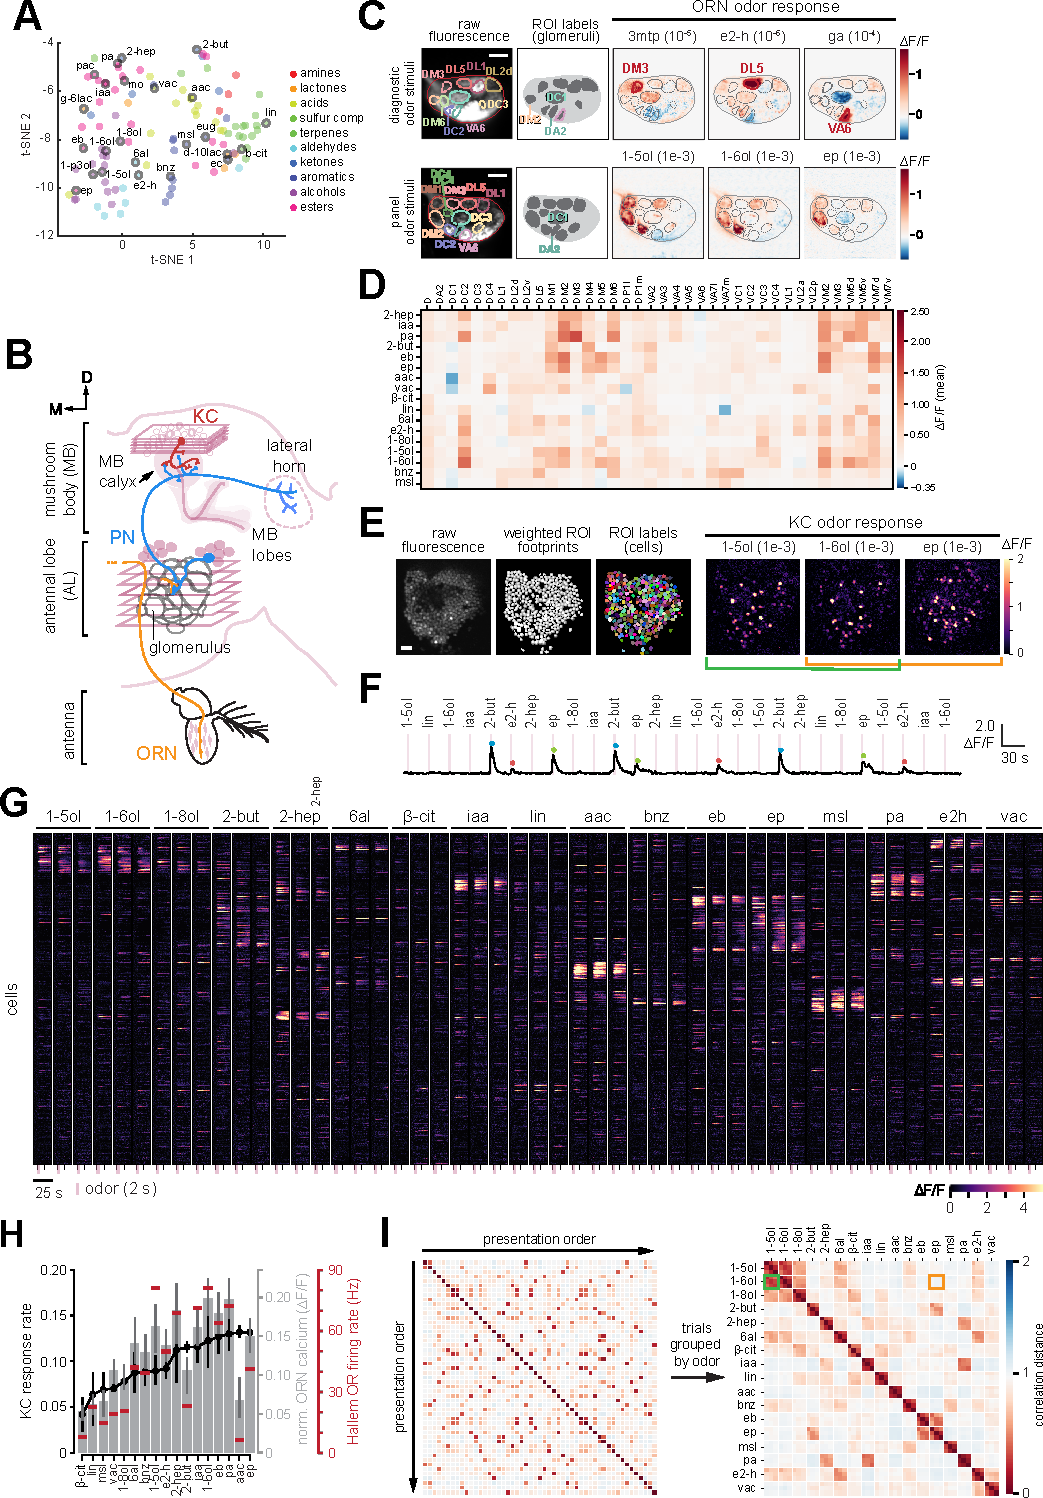
\includegraphics[height=0.8\textheight]{1}

\mycaptionof{figure}{Population representations of odor in the fly MB at cellular resolution}{}
\label{fig:1}

\mysubcaption{A}{%
$t$-SNE embedding of 109 odors based on the patterns of activity they elicit across 24 fly ORs in the Hallem dataset.
A subset (open gray symbols) spanning the odor space was selected for measurement in the MB.
}

% TODO happy with this?
\mysubcaption{B}{%
Imaging volumes comprising \textasciitilde11 planes through the KC soma layer capture the activity of >85\% of KCs in an MB (top), or \numrange{9}{10} planes covering all \textasciitilde50 glomeruli in the AL (middle).
}

% TODO TODO say genotype? how/where?
% TODO TODO was it from one fly?
% TODO TODO TODO what was size of scale bar? say so
\mysubcaption{C}{%
Example ORN terminal trial-averaged \DeltaFOverF{ }odor responses in two example planes from one fly (right three columns).
All glomeruli identified in each plane are shown collectively across the left two columns.
Top: responses to three ``diagnostic'' odors, with the target glomerulus for each labeled in red.
Bottom: responses to three example odors, with 1-pentanol and 1-hexanol exhibiting more similar responses than either does to the more structurally distant ethyl propionate.
See \Crefwithbackref{fig:s1} for example volumetric responses to the full 24-odor diagnostic panel and identified ROIs, and \Crefwithbackref{fig:s2} for mean responses to this panel for all our individual ORN flies.
See \Crefwithbackref{table:diagnostic_odors} for odors and concentrations.
}

\mysubcaption{D}{%
Mean ORN terminal response for each responsive glomerulus to this first 17-odor panel ($n{=}9$).
See \Crefwithbackref{fig:s3} for means, SDs, and per-glomerulus sample sizes for all of our ORN terminal and PN dendrite data.
}

\mysubcaption{E}{%
Left: baseline fluorescence (left), weighted ROI masks of KCs (middle), and ROI labels corresponding to individual KCs (right) from a single imaging plane in an MB.
Right: odor-evoked patterns of KC activity in response to 1-pentanol, 1-hexanol, and ethyl propionate.
Scale bar, \qty{10}{\micro\metre}.
}

\mysubcaption{F}{%
Example odor-evoked calcium signals in an imaging block from a single KC.
}

\mysubcaption{G}{%
Population representations in \textasciitilde\num{1800} KCs to 17 odors in the MB from a representative fly.
Each row is a cell and each column is a trial.
Cells are sorted by odor tuning.
}

% used to be S1B, but now gray bars which were Hallem are my "normalized" ORN data, w/ new red markers + y-label for Hallem OR firing rate
% TODO still n=4 for remy's KC data here?
% TODO happy with this?
\mysubcaption{H}{%
Comparison of KC response rate (mean and 95\% CI, $n{=}4$ flies; black), normalized mean (across glomeruli) ORN terminal \DeltaFOverF{ } (mean and 95\% CI, $n{=}9$ flies; gray), and mean evoked OR firing rate (across receptors) in the Hallem dataset to each odor (red).
}

\mysubcaption{I}{%
Matrix of pairwise correlation between KC population responses in individual odor trials, where trials are shown in presentation order (left) or grouped by odor (right).
KC responses elicited by 1-hexanol were more similar to those elicited by 1-pentanol (green) than by ethyl propionate (orange).
% TODO remove abbrevs here and refer to table? or be consistent in chap:natmix
% TODO TODO remove genotypes and just refer to table (or add for ORN flies)
Flies had genotype 20xUAS-nls-OpGCaMP6s-p10 (III)/+; OK107-Gal4 (IV)/+.
% TODO TODO be consistent w/ these abbrevs
Odors are 1-pentanol (1-5ol), 1-hexanol (1-6ol), 1-octanol (1-8ol), 2-butanone (2-but), 2-heptanone (2h), hexanal (6al), \BCit\,(B-cit), isoamyl acetate (IaA), linalool (Lin), acetic acid (aa), benzaldehyde (benz), ethyl butyrate (eb), ethyl propionate (ep), pentyl acetate (pa), trans-2-hexenal (t2h), and pentanoic acid (va).
}
\end{longcapfigure}

In the arc of sensorimotor transformation, representations of odor identity encoded in KC activity patterns represent the output from the sensory arm of the pathway that is flexibly coupled to distinct downstream outputs and behaviors\cite{MBLearningBehaviorReview}.
Thus, we began by investigating representations of odor in the MB.
% TODO is italics only for full species names? say something other than (or delete) "In Drosophila"? (word document working copy has italics here)
The \textit{Drosophila} olfactory circuit is the most comprehensively mapped metazoan olfactory system, with the tuning of approximately half of the odorant receptors to a large panel of 109 odors described by the Hallem dataset\cite{Hallem2006}.
We selected 24 monomolecular odors that spanned OR input space (\crefwithbackref{fig:1:A}) and investigated the extent to which those input relationships are maintained in MB representations of the odors.
% TODO does this sentence really fit here?
Between 9 and 17 odors were measured together in the same MB. 

% TODO TODO should all (any?) genotypes be italic? (this OK107-Gal4 reference is in word doc)
We used in vivo volumetric two-photon microscopy to image odor-evoked calcium signals in the MB of flies expressing nuclear-localized GCaMP6s selectively in KCs (directed by the \textit{OK107-Gal4} driver\cite{OK107}) (\cref{fig:1:B}).
In pilot experiments using cytoplasmic GCaMP6f as the calcium reporter, the small size (\textasciitilde\qtyrange{2}{3}{\micro\metre}) and tight packing of KC somata (\cref{fig:1:E}) presented challenges for reliable cellular segmentation and pixel assignment to individual KCs over the course of an imaging session, with poor trial-to-trial reliability in odor panels larger than 8 odors. 
To expand the size of odor panels that could be evaluated in a single brain, we measured KC activation using nuclear calcium, which has slower response dynamics, but strongly correlated response amplitudes, compared to cytoplasmic calcium\cite{NuclearVsCytoplasmicCalcium1,NuclearVsCytoplasmicCalcium2}.
Localization of the calcium indicator to nuclei resulted in a several pixel gap between KCs that facilitated reliable cellular segmentation (\cref{fig:1:E}).

Flies were presented odors while imaging with fast-scanning through the KC cell body layer, and odor-evoked KC signals were extracted from volumetric movies using the Suite2p pipeline\cite{Suite2p}.
In brief, after registration across frames of each functional movie in each plane to correct for motion, regions of interest (ROIs) representing each KC were extracted (\cref{fig:1:E}).
Although cell detection in Suite2p is usually neural activity-based, we used settings that extracted \textasciitilde90\% (\textasciitilde\numrange{1800}{2000} cells) of the expected number of KCs in each MB using maps of the mean correlation of pixel fluorescence with its nearby pixels and anatomical priors of the expected size and shape of cell ROIs.
Since KC odor responses are sparse and many KCs do not respond to any odor in even a relatively large panel, this adjustment was important to allow good estimates of KC response rates.
For a subset of experiments, odor responses were registered to KCs across different functional movies collected from the same MB by alignment of ROIs to 3D anatomical models of KC somata constructed from high-resolution structural images through the MB.

Reproducible odor-specific response dynamics were observed in some cells (\cref{fig:1:F}), but, given the overall slow kinetics of nuclear-localized GCaMP6s, we focused our analysis of this data on the peak amplitude of odor-evoked responses.
KC population responses were stable, odor-specific, and reliable across repeated trials of the same stimulus (\cref{fig:1:G},\subref{fig:1:I}).
The relationship between odor representations in MB coding space was quantified using the correlation distance $1-r$, where $r$ is the Pearson's correlation between the vector of KC responses to each odor.
% TODO delete? still have comparison w/ cosine vs pearson? (in one version of supplement yes. not sure if it's only missing b/c i edited out as much as i did, to remove hemidraw. restore S1H (would prob be leterred S1F now)? doesn't seem it's just me. old 1F,G are now S5A,B (which i edited out)
% now that i'm using version of S4 with F-H (hemidraw mostly), don't have to say "data not shown" here
% TODO TODO actually, i probably won't as it seems the goal was to move a subset into start of S5 (A/B), and drop rest
Quantifying odor relationships using other metrics such as cosine distance yielded similar results (data not shown). %(e.g. \cref{fig:s4}H).
When we computed the correlation distance between the KC response vector for every pairwise combination of trials in an experiment (\cref{fig:1:I}, left) and reordered the distance matrix to group together trials by odor, we observed that KC responses from trials presenting the same odor were very similar (on-diagonal blocks, \cref{fig:1:I}, right).
These results demonstrate the reliability of KC odor responses across multiple presentations spanning the time course of an experiment.
As expected, the pairwise correlation distance between odors reflected the qualitative similarity of their respective KC response patterns (\cref{fig:1:E},\subref{fig:1:I}), with visually similar activity patterns corresponding to short odor distances.

The percentage of KCs responding to each odor was similar in each MB, ranging from \textasciitilde\qtyrange{5}{13}{\percent} depending on the odor (\cref{fig:1:H}).
% TODO TODO TODO talk to remy about this (slacked her about it)
When compared against mean OR activity for each odor, estimated by averaging the firing rates evoked by each odor across all ORs in the Hallem dataset, KC response rate was not significantly correlated with mean ORN response strength (\cref{fig:1:H}, Spearman's $\rho{=}0.48$, $p{=}0.05$).
However, we note that the Hallem dataset underestimates ORN population responses to acids and amines since it does not include odorant receptors from the ionotropic receptor (IR) family\cite{IRs}.

Overall, KCs were narrowly tuned, with most cells responding to two or fewer odors, and a significant fraction (\textasciitilde40\%) responding to no odor in a 17-odor panel.
% TODO TODO is "more broadly tuned" even accurate? what point is 3F actually making?
However, compared against modeled KC responses, observed odor responses in KCs were more broadly tuned (\crefwithbackref{fig:3:F}).
This result is consistent with observations that existing MB models poorly predict KC response rates to narrowly activating odors that selectively excite only one or very few ORN classes (e.g., \BCit{ }or methyl salicylate, \crefwithbackref{fig:s5:C}).
These results confirm that KC responses are sparse and selective.
They also indicate that current assumptions about MB circuit properties do not fully account for observed KC response rates to all odors, particularly for narrowly activating odors.

\subsection{Representations of odor in the MB are structured and invariant across individuals}
In most circuits of the fly brain, neuronal connectivity is invariant across individuals, but the MB is distinct in that the wiring of PN inputs is probabilistic: each of the \textasciitilde\num{2000} KCs, the principal neurons of the MB, integrates input from a quasi-random subset of PNs comprising \textasciitilde10\% of the \textasciitilde50 olfactory glomeruli in the system.
As the number of possible glomerular combinations far exceeds the number of KCs in any given MB, stereotyped KC connectivity, defined by a specific set of synaptic inputs, does not exist across individual MBs.
Indeed, a small set of genetically defined KCs labeled by a sparse Gal4 driver did not exhibit stereotyped odor tuning\cite{MBResponseStereotypy}.
However, feedforward network models that assume random divergent connectivity between second- and third-order olfactory layers predict that, while third-order olfactory responses will be comparatively decorrelated, they will otherwise maintain relative pairwise odor relationships present in the prior layer.
Thus, these models predict that odor relationships encoded in third-order olfactory representations will be invariant across different instantiations of the network (i.e., MBs), with preserved odor relationships that are predictable from the tuning of ORN inputs.

% Figure 2 - MB representational space is structured and invariant across individuals
% {
\begin{longcapfigure}
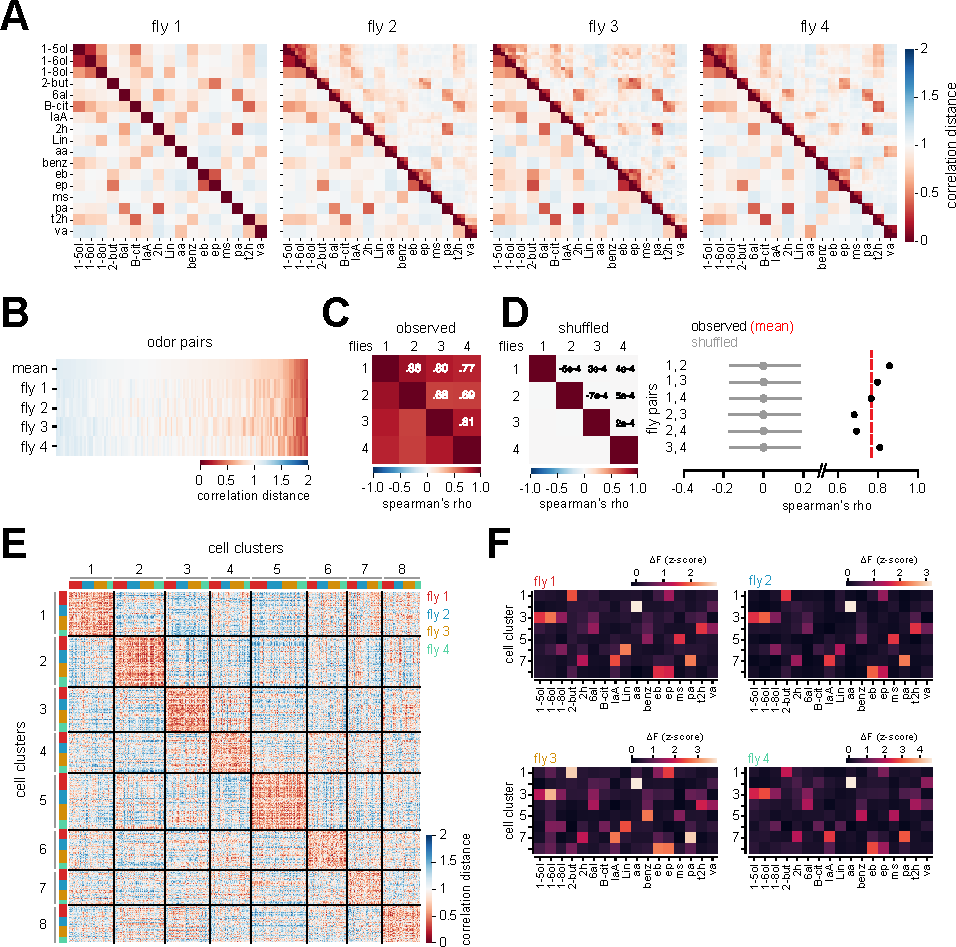
\includegraphics[width=\textwidth]{2}
\mycaptionof{figure}{MB representational space is structured and invariant across individuals}{}
\label{fig:2}

\mysubcaption{A}{%
Correlation distance matrices for four different flies showing pairwise relationships between KC population responses in individual odor trials (upper triangles) or in trial-averaged responses for each odor (lower triangle).
}

\mysubcaption{B}{%
Correlation distance between trial-averaged KC responses for every odor pair for the four flies in \textbf{(A)}.
Odor pairs are shown in the same order in each row, arranged by their mean correlation distance across the four flies.
Odors that evoke similar KC response patterns in one fly tend to also elicit similar response patterns in other flies.
}

% TODO TODO is this actually the (sorted) rows of B? (maybe it's a bit redundant if we are just talking about sorting as part of spearmans? but is that correct?)
\mysubcaption{C}{%
Spearman's rank correlation between the rows of \textbf{(B)} (i.e., between flies), evaluating the similarity of the rank ordering of odor pairs between flies according to their representational distance in KCs.
}

\mysubcaption{D}{%
Left: same as \textbf{(C)}, but for shuffled data where odor responses were randomized by permuting the columns of the cell x odor response matrix for each fly.
The matrix shows the mean Spearman's correlation across \num{10000} shuffles.
Right: observed Spearman's correlation (black) and the mean and 95\% CI of the Spearman's correlation across \num{10000} shuffles (gray) for each fly pair.
Red dotted line marks the mean observed Spearman's correlation ($\rho{=}0.76$).
}

\mysubcaption{E}{%
Matrix of pairwise correlation distances (over odors) between every KC in the four flies in \textbf{(A)} that responded to at least one odor.
The distance matrix was ordered by spectral clustering on the mean odor response vector of each cell.
Each response cluster contained KCs from every fly.
}

% TODO TODO do similar clustering (/my own response class sorting) of model KCs responding to megamat, to compare model vs KC cells? (+ my own response class sorting of remy's KC megamat responses)
\mysubcaption{F}{%
Mean odor response profiles across KCs in each response cluster for each fly.
KCs with conserved odor tuning profiles were found in every MB.
}
\end{longcapfigure}
% }

To evaluate these ideas, we compared the correlational structure of odor representations encoded in KC activity patterns in multiple flies.
% TODO add back S2A, if remy has it and it makes sense
We found that the relationships between odors in MB representational space were indeed structured and invariant across individual brains (\crefwithbackref{fig:2:A}), consistent with prior work\cite{Endo2020}.
We evaluated the similarity of the correlational structure across MBs using pairwise comparisons of the ordering of odor pairs in each MB according to their ranking by correlation distance (\cref{fig:2:B}-\subref{fig:2:C}).
% TODO delete?
%The observed distribution of MB-MB correlations (Spearman's $\rho\!=\!0.76\!\pm\!0.06$) was significantly different from shuffled controls
% TODO some solution i'm generally happy with? liked the rho formatting above more than the commented line below (but previously preferred just {=}) (go back to {=}? use that most places...)
% TODO use \num for both p-value expressions below?
The observed distribution of MB-MB correlations (Spearman's $\rho{=}\,0.76{\pm}0.06$) was significantly different from shuffled controls (\cref{fig:2:D}, $p\,{<}\,10^{-4}$).
% TODO TODO move discussion of (what is now 3C) after model has been introduced?
Also, the correlation distance between specific pairs of odors was consistent across individual MBs: odors that evoked similar KC response patterns in one fly tended to also have similar KC responses in other flies, and the same was observed for odors that evoked dissimilar representations (\cref{fig:3:C}; $p{=}10^{-186}$, one-way ANOVA).
Finally, we combined all KCs that responded to one or more odors from four different flies and clustered the KCs based on each cell's odor response tuning to a panel of common odors.
This analysis identified reliable response types with specific odor tuning profiles, and each response type was found in each of the four flies (\cref{fig:2:E}).
For instance, KCs that were strongly co-tuned to 2-heptanone, isoamyl acetate, and pentyl acetate were reliably observed in every MB (\cref{fig:2:F}).
These results demonstrate that the structure of the representational space of odors is highly conserved across individual MBs in the fly.

\subsection{Odor distances in MB coding space diverge from odor relationships predicted by a random feedforward network model}

% Figure 3 - Odor relationships in MB representational space deviate from predicted relationships in a random feedforward network
% {
\begin{longcapfigure}
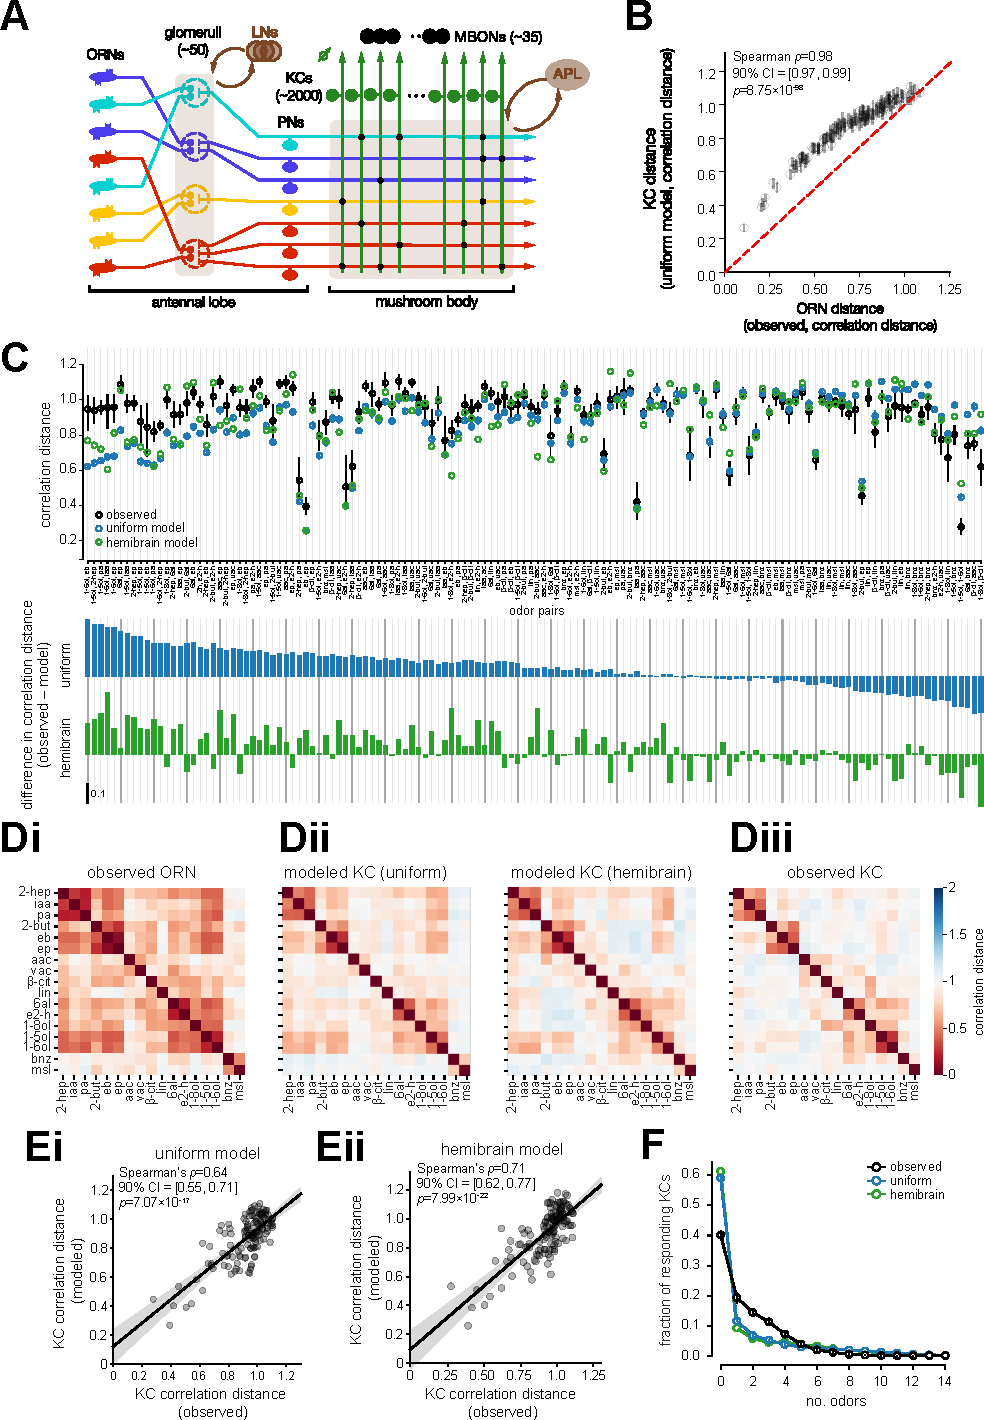
\includegraphics[width=\textwidth]{3}
% TODO has this (or any other) working caption label changed?
\mycaptionof{figure}{Odor relationships in MB representational space deviate from predicted relationships in a random feedforward network}{}
\label{fig:3}

\mysubcaption{A}{%
Schematic of the fly olfactory network.
}

\mysubcaption{B}{%
Comparison of odor-pair correlation distances ($1 -\text{Pearson's } r$) in the uniform KC model with those in observed ORN coding space (black symbols; $n{=}136$ pairs from 17 odors).
% TODO TODO also update working text to not say mean is over a different # of MBs than the errorbars
Each circular marker is the mean across 20 simulated mushroom bodies (MBs); each MB had an independently generated PN–KC connectivity matrix in which every glomerulus was drawn with equal probability.
% TODO double check this isn't actually what figure is still showing
%Error bars span the $25^{th}{-}75^{th}$ percentiles across those 100 models. 
Error bars within each marker are 95\% CI across these 20 simulated MBs.
Red dashed line shows unity.
The uniform model systematically decorrelated odor pairs, most strongly for odor pairs that are similar in ORN space, while closely preserving the rank ordering of ORN odor–odor distances (Spearman's $\rho{=}0.98$, $p{=}\num{8.8e-98}$, 90\% CI \numrange{0.97}{0.99}).
}

% TODO is S2A actually correct in remy/betty's current supplemental fig numbering? (doesn't seem so) (delete S2A stuff unless remy produces a figure / table  that has this. i made my own S7 for this)
% TODO and is my s7 making same point as intended with this reference (showing N per pair)?
% (i assume so?)
\mysubcaption{C}{%
Top: Scatter plot of correlation distances (mean and 95\% CI) between KC responses for each odor pair, averaged across all flies in which the odor pair was sampled ($n{=}4{-}18$ flies, see Supplemental \Crefwithbackref{fig:s7}). %see Supplemental Figure 2A).
A one-way ANOVA showed there was a significant difference in the odor–odor correlation distance between different odor pairs ($F\text{-statistic}{=}17.57$, $p{=}\num{1.1e-187}$), consistent with odor–odor relationships being reliable across MBs in different flies.
The correlation distances between predicted KC responses for odor pairs in the uniform and hemibrain models are plotted for reference (see \textbf{Dii}).
For the uniform model, error bars are 95\% CI across the first 20 instantiations of the model.
Odor pairs are ordered by the difference between observed and uniform-model distances.
% TODO delete this line if i update plot colors (see below)
Lower: bar plots show the difference between observed and model KC correlation distances (observed - model) for each odor pair, for the uniform (top) and hemibrain (bottom) connectivities.
}

% TODO TODO restore this line if i update the colors to match, as remy did
%Lower: bar plots show the difference between observed and model KC correlation distances (observed - model) for each odor pair, for the uniform (top, blue) and hemibrain (bottom, green) connectivities.

\mysubcaption{D}{%
Matrix of pairwise correlation distances ($1 - \text{Pearson's } r$) between:
\textbf{i)} observed ORN responses;
\textbf{ii)} (left) predicted KC responses in the uniform model (left) or hemibrain model (right); or
\textbf{iii)} observed KC responses
for 17 odors.
% TODO cite ann's paper as previous case that does this? or say how it's similar to dropping silent KCs (or do we not [explicitly...]?)?
Model KCs that responded to none of the odors were excluded from correlation calculations.
}

% NOTE: my figure still has E and F swapped, relative to remy's last version, but i think she's on board to change it
\mysubcaption{E}{%
Comparison of observed and modeled KC odor spaces: each scatterplot shows correlation distance ($1 - \text{Pearson's }r$) between KC responses to each odor pair, modeled versus observed.
\textbf{i)} Uniform model, in which every glomerulus is equally likely to connect to each KC.
\textbf{ii)} Hemibrain model, which uses PN-KC connections from the hemibrain EM dataset.
Each point represents one odor pair ($n{=}136$); observed KC distances are averaged across flies ($n{=}4{-}18$); uniform model KC distances are averaged across 100 instantiations of the model.
The line shows the linear fit between modeled and observed distances, with 95\% CI of the fit shaded.
Spearman's $\rho$ between modeled and observed distances:
uniform model, $\rho{=}0.64$ (90\% CI \numrange{0.55}{0.71}; $p{=}\num{7.1e-17}$);
hemibrain model, $\rho{=}0.71$ (90\% CI \numrange{0.62}{0.77}; $p{=}\num{8.0e-22}$).
% TODO TODO is this CI (on the rho) actually from bootstrapping across odors pairs? check code
CIs were computed from a bootstrap over odor pairs.
}

\mysubcaption{F}{%
Observed fraction of KCs (mean and 95\% CI) responding to the indicated number of odors for a panel containing 17 odors.
The distributions of the fraction of modeled KCs responding to different numbers of odors in the uniform and hemibrain models (as in \textbf{(Dii}) are plotted for comparison.
}
\end{longcapfigure}
% }

To compare the observed structure of MB representational space to what is predicted by a feedforward random network, we modeled KC population responses by adapting a previously described spiking model of the fly olfactory circuit\cite{Kennedy2019} (\cref{fig:3:A}).
% TODO TODO TODO actually write methods section on this (+ link to it specifically)
We scaled our mean ORN \DeltaFOverF{ }imaging data by a factor to approximately convert into units of $\Delta\text{ spike rate}$ (see Methods), to work with this model that previously used the spike rate Hallem dataset\cite{Hallem2006} as input.
These ORN firing rates were propagated through the existing AL section of the model to generate PN firing rates, which were used as input to a population of \num{1837} spiking KCs.
% TODO TODO TODO discuss how ann did both spike-rate and poisson PN inputs, but we just use the spike-rate as she did for many things?
% maybe just in methods?
% TODO TODO just say 7 here, as we don't introduce hemibrain till later?
KCs were modeled as leaky integrate-and-fire units with a small number of input sites, typically \textasciitilde\numrange{5}{7} dendritic claws, that each receive input from a single PN bouton.
Under assumptions of random feedforward connectivity, the matrix of PN-KC connections in each model instantiation was created by assigning each KC claw a single glomerular input, with all glomeruli having an equal likelihood of being drawn (`uniform' model).
KC activity was normalized by global feedback inhibition from the non-spiking GABAergic APL.
% TODO TODO change below for accuracy?
% say 9.15%? or ~9.15% (since theres that 10% relative tolerance)? "which matches response rates we determined on our first set of 17 odors"?
% (9.15% was determined from response rates we calculated on KCs to megamat, and then was ALSO USED FOR VALIDATION2 MODELING)
KC spiking thresholds and \APLKC inhibitory weights were tuned to achieve a mean KC response rate of \textasciitilde10\% across odors (see Methods), which matches experimental observations.

The correlation between modeled KC responses for specific odor pairs was indeed consistent across 20 simulated MBs with different, independently drawn random PN-KC connectivity matrices (\cref{fig:3:B}, error bars are 95\% CI across simulations).
However, the observed structure of odor representations in KC coding space was only partially predicted by the feedforward random model, with the observed relationship between odors deviating significantly from model predictions for many odor pairs (\cref{fig:3:C}-\subref{fig:3:E}).
In particular, observed pairwise odor relationships were overall more decorrelated than those predicted from modeled KC populations (\cref{fig:3:E}i).
% TODO TODO replace w/ discussion of sensitivity analysis now? or add a bit about that? mentioned anywhere yet? maybe just do in methods?
Adjusting fit parameters to yield a lower mean KC response rate of 5\% across odors did not appreciably affect the systematic overprediction of the degree of correlation between odor representations, nor did it affect the rank order of predicted odor-odor correlation distances (data not shown).

% TODO go back to referring to just s4a in first part here? i just didn't really think it made sense... but if we must call out each letter explicitly... idk
Recent analysis using large-scale EM-level reconstructions of part of the Drosophila brain at synaptic resolution (\crefwithbackref{fig:s4}) revealed that the wiring of PN inputs to KCs is not fully random\cite{MBConnectomeInsights,CommunityPNs}.
Indeed, analysis of the complete matrix of PN-KC connectivity from two independently reconstructed fly brains confirmed that PN inputs from specific subsets of glomeruli are overly convergent onto individual KCs, and the structure of this biased input onto KCs is similar between two MBs from different flies\cite{CommunityPNs} (\cref{fig:s4:B}-\subref{fig:s4:E}).
% TODO edit fig to add separate letter for this LHN matrix? (then also restrict ref above to range ending in previous letter)
We also observed that the glomerular input structure to KCs bears significant similarity to the structure of glomerular input to third-order olfactory neurons in the lateral horn (\cref{fig:s4:E}), a brain region dedicated to innate odor processing in which neurons have stereotyped connectivity and tuning\cite{LHNStereotypy,LHFruitPheromoneSegregation}.

% TODO TODO TODO continue updating references / text from here <<<<<<<<<<<<<<<<
% TODO restore (at least commented) some of the hemidraw text from working copy first?
% TODO TODO TODO either here or in methods, say that goal was to get a number of claws by picking divisor we did, and it gave us something ~7, like past work
% TODO "is defined by dividing the connectome synapse count by a factor which produces a similar number of `claws' as the 7 we used for the prior `uniform' model"? or just leave to methods?
To assess the possible impact of structured olfactory input on MB odor representations, we predicted KC odor responses in a variant of our model (`hemibrain') where the PN-KC connectivity is defined from lightly-processed synapse counts measured in the hemibrain connectome (see Methods).
% TODO regarding "did not meaningfully improve":
% actually do a statistical test, or is it really sufficient to compare CI on spearman rhos (which do overlap at 90% CIs)?
Incorporating the hemibrain PN-KC connectivity did not meaningfully improve model predictions of observed KC odor relationships (\cref{fig:3:D},\subref{fig:3:E}).
% TODO still mention hemidraw here a bit? (if using S3 with F-H describing it)? or leave to methods?
This result indicates that observed biases in PN-KC connectivity are unlikely to account for much of the differences between observed and predicted KC odor responses; and suggests additional sources of structure are present in the olfactory circuit that mediate the observed transformation of odor representations from the periphery to the MB.
% old paragraph that also discussed hemidraw, for reference
% (figure references may not be accurate currently)
\iffalse
To assess the possible impact of structured olfactory input on MB odor representations, we predicted KC odor responses in the model under conditions in which the PN-KC connectivity matrix was drawn according to the observed frequency of PN boutons corresponding to each glomerulus in the hemibrain dataset (“hemidraw”) or in which the experimentally reconstructed hemibrain PN-KC connectivity matrix was directly implemented (“hemibrain”) (see Methods). Neither adjustment to PN-KC connectivity improved predictions of odor relationships in KC representational space (Figure 3C, 3Dii, S3F-H) relative to observed relationships; in fact, predicted responses for most odor pairs trended towards being more correlated compared to the uniform model. These results indicate that observed biases in PN input connectivity to KCs are unlikely to account for the differences between observed and predicted KC odor responses; they suggest additional sources of structure are present in the olfactory circuit that mediate the observed transformation of odor representations in the MB.
\fi

\subsection{Reorganization of representations of odor in the MB around odor relationships in natural sources}

% Figure 4 - Reorganization of odor representations in the fly MB reflects odor relationships in natural sources
% {
\begin{longcapfigure}
% don't really need \centering since using full textwidth, and don't want it for captions anyway (esp to be consistent w/ continuation on next page)
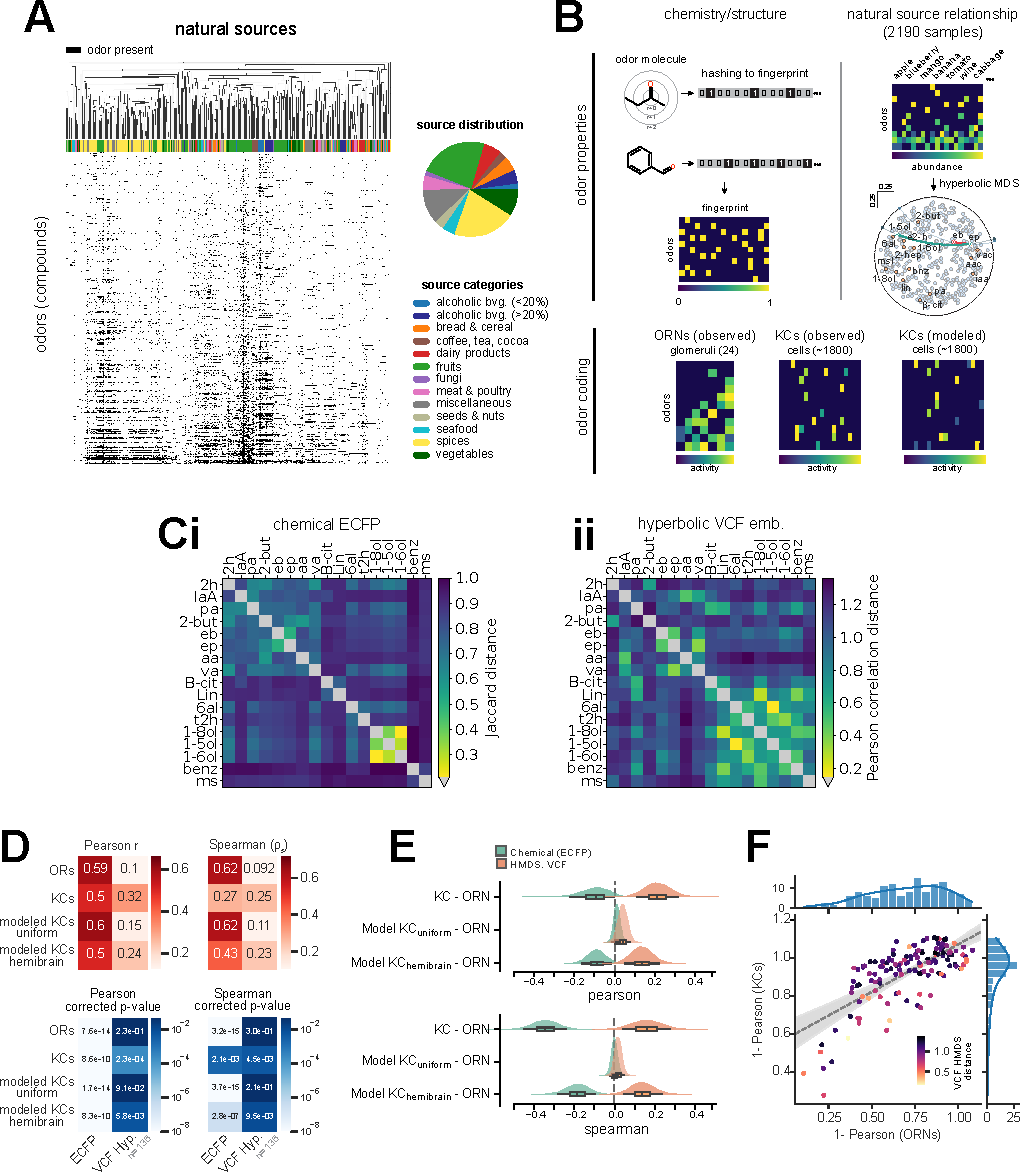
\includegraphics[width=\textwidth]{4}
\mycaptionof{figure}{Reorganization of odor representations in the fly MB reflects odor relationships in natural sources}{}
\label{fig:4}

\mysubcaption{A}{%
Distribution of odors (monomolecular compounds) in a literature-based database of the volatile headspace composition of many natural food odor sources.
The pie chart shows the distribution of odor sources in each food category.
}

\mysubcaption{B}{%
Schematic summary of datasets for comparing the properties of odors (top) with their different neural representations (bottom).
% TODO did we define ECFP earlier? should we?
Top left, each odor is represented as a binary ECFP fingerprint; structural dissimilarity between odor compounds is computed as the Jaccard distance between fingerprint vectors.
Top right, odor compounds were embedded by hyperbolic MDS ($D{=}3$) to fit odor–odor dissimilarities computed as $1-\text{Pearson's }r$ between natural-source feature vectors.
The Poincaré disk shows all 452 embedded compounds (light blue), with the 17 odors used in \textbf{C--F} highlighted (orange).
}

% TODO happy with this?
\mysubcaption{C}{%
Non-neural odor–odor dissimilarity matrices for the 17 odors, with odors in the same order as matrices in \Cref{fig:3:D}, computed on:
\textbf{(Ci)} chemical structures, as Jaccard distance between binary ECFP fingerprint, and
\textbf{(Cii)} natural source space, as hyperbolic distance between embedded compound distributions from VCF.
}

\mysubcaption{D}{%
Summary of correlations (upper) and corrected $p$-values (lower) for comparisons between observed ORN, observed KC, or modeled KC (uniform or hemibrain) odor–odor relationships and those in chemical space (Jaccard distance between ECFP fingerprints) or natural source space (hyperbolic distance in the embedded VCF space).
Pearson's $r$ (left) and Spearman's $\rho$ (right); $n{=}136$ odor pairs.
$p$-values from $t$-test, corrected by Benjamini-Hochberg.
}

\mysubcaption{E}{%
Bootstrapped difference of correlations between odor–odor distances in observed ORN coding space and in observed or modeled KCs (uniform or hemibrain), against chemical fingerprint distances (green) and embedded natural source distances (orange).
Pearson's $r$ (top) and Spearman's $\rho$ (bottom) correlations are shown for \num{5000} resampling draws of the 136 odor pairs with replacement, with 90\% CI ; boxes, interquartile range and mean; whiskers, CI.
Positive values indicate that a KC space is more closely aligned to the reference space (chemical structure or natural source)
}

\mysubcaption{F}{%
Observed KC odor–odor dissimilarities vs. observed ORN odor–odor dissimilarities ($n{=}136$ pairs).
Colors indicate hyperbolic distance between odors in the embedded natural source space.
Dashed line shows OLS fit; marginal histograms show distribution of dissimilarities along each axis.
Odor pairs that are close in embedded natural source space tend to fall below the fit: they are more similar in KC coding space than their ORN distances would predict.
}
\end{longcapfigure}
% }

Comparisons of odor coding in the ORN input layer and in the MB showed that, although the representations of most pairs of odors were substantially decorrelated, as expected, some odor pairs were comparatively less decorrelated between the ORN and MB layers.
This transformation resulted in a significant regrouping of odor relationships in ORN versus MB coding space.
For instance, the odors 2-heptanone, isoamyl acetate, and pentyl acetate emerged as a representational cluster in KC coding space, distinct from other odors in the panel, whereas the representation of each of these odors is similar to many others in the ORN representations (\cref{fig:3:D}i,iii).

To better understand the functional implications of this reorganization, we asked how odor representations at different stages of olfactory processing relate to the properties of the odors, focusing in particular on their chemical properties and on how they are correlated across natural odor sources.
% TODO TODO add RDkit citation later. DOI depends on specific version used
% https://www.rdkit.org/docs/Overview.html
% e.g. https://doi.org/10.5281/zenodo.591637 (<- may have a list of them by version?)
% recommended citation is "RDKit: Open-source cheminformatics. https://www.rdkit.org"
Each odor was represented as an extended-connectivity fingerprint (ECFP6, i.e. extended connectivity fingerprint, a circular fingerprinting method with diameter 6) computed from its canonical SMILES string using the chemoinformatics library RDKit (\crefwithbackref{fig:4:B}, upper left)\cite{ECFP}.
The chemical fingerprinting approach encodes each molecule as a binary vector in which each bit denotes the presence of a particular substructure of a particular size.
The structural similarity between two odor compounds was computed as the Tanimoto coefficient ($1 -\text{ Jaccard distance}$) between their binary fingerprint vectors (\cref{fig:4:C}i).

% TODO and only abbreviated "D. ..." in abstract so far. be consistent about that?
\textit{D. melanogaster} is an ecological generalist and human commensal\cite{DrosophilaEcology}; as a starting point for understanding the structure of natural odor space for Drosophila, we used a database of the headspace volatile profiles for many food odor sources, compiled from thousands of published chemical datasets primarily from the food and flavor science literature (\cref{fig:4:A}).
The odor sources are biased towards fruits, plants, and vegetables, but also includes other common human foods such as alcoholic beverages, meat, and dairy products.
The database comprises thousands of samples measured from \num{1445} types of natural sources (apple, tomato, wine, etc.) and contains over \num{10000} monomolecular volatiles.
Like other datasets profiling the chemical volatiles emitted from natural sources\cite{OlderFoodVolatileReview}, the majority of odorants occur sparsely in a small number of sources, though a significant minority of odors are present broadly across many sources (\cref{fig:4:A}).

Recently, we showed that the use of hyperbolic coordinates to embed the concentrations of individual monomolecular odorants as they occur in natural odor sources better captures odor relationships in the space of natural sources, compared to embeddings that use Euclidean metrics\cite{HyperbolicOdorsBees,HyperbolicOdors}.
The use of hyperbolic distance metrics is motivated by their ability to approximate the hierarchical tree-like relationship between volatiles in natural headspace profiles, the result of correlations in molecular composition driven by structured biochemical networks in natural sources.
% TODO Zhou2021 appropriate? establish part of method?
We used hyperbolic multidimensional scaling to embed odors from the literature-based natural source database into a three-dimensional hyperbolic space (\cref{fig:4:B}, upper right)\cite{Praturu2022,Zhou2021}.
We found that the correlational structure of odorant compounds in the headspace profiles of our natural source database was well-fit by a hyperbolic embedding with negative curvature ($dim{=}3$; $R_{max}{=}\num{3.197}$).
Odor distances in the hyperbolic embedding have been shown to better capture the correlational structure of the abundance of odors across natural sources compared to equivalent distances computed from a Euclidean embedding\cite{Ghaninia2022,Zhou2018}.
Thus, we used hyperbolic distances as a metric of odor relationships in natural source space. 

For each of the 136 unique odor pairs, we compared their representational distance in ORN or KC coding space with their relationship in chemical descriptor space or natural source space (\cref{fig:4:C}) with Pearson and Spearman's rank correlation.
We found that pairwise odor distances in chemical structure space were more strongly correlated with distances in ORN coding space ($r{=}0.592$, $p{=}\num{9.0e-14}$, Spearman's $\rho {=}0.618$, $p{=}\num{3.8e-15}$) than KC coding space ($r{=}0.504$, $p{=}\num{1.0e-9}$, Spearman's $\rho {=}0.272$, $p{=}\num{2.3e-3}$), while pairwise distances in natural source space were more strongly correlated with odor pair distances in KC ($r{=}0.317$, $p{=}\num{2.6e-4}$, Spearman's $\rho {=}0.252$, $p{=}\num{4.9e-3}$) space than ORN space ($r{=}0.105$, $p{=}0.23$, Spearman's $\rho {=}0.092$, $p{=}0.29$). 

We also evaluated the relationship of odor properties to odor distances in modeled KC coding space, with the same uniform and hemibrain model variants discussed previously.
Uniform modeled KC distances correlated with chemical structure distances ($r{=}0.604$, $p{=}\num{2.0e-14}$; Spearman's $\rho {=} 0.617$, $p{=}\num{4.3e-15}$) about as strongly as observed ORN distances did ($r{=}0.592$; $\rho {=} 0.618$) and more strongly than observed KC distances did.
The same pattern held for natural source space: the uniform model ($r{=}0.148$, $p{=}\num{0.090}$; Spearman's $\rho {=} 0.110$, $p{=}\num{0.21}$) tracked the ORNs ($r{=}0.105$; $\rho {=} 0.092$) more closely than the observed KCs, though its correlations were marginally higher.
Neither the observed ORNs nor the uniform KC model were significantly correlated with natural source distances computed from the hyperbolic embedding.

Hemibrain model KC distances fell between the observed ORN and KC values for the chemical structure comparison under the Spearman rank correlation (Spearman's $\rho {=} 0.433$, $p{=}\num{3.3e-7}$).
Its Pearson correlation with chemical structure ($r{=}0.504$, $p{=}\num{9.8e-10}$) was indistinguishable from that of the observed KCs ($r{=}0.504$).
For natural source space, it fell between the observed ORN and KC values for both space metrics ($r{=}0.240$, $p{=}\num{6.0e-3}$; Spearman's $\rho {=} 0.230$, $p{=}\num{1.0e-2}$).

The comparisons between correlation coefficients are not directly tested by their individual $p$-values.
We therefore computed the difference in correlation ($\Delta\rho$) with each reference space between KC and ORN coding spaces, by resampling the 136 odor pairs with replacement over \num{5000} iterations (\cref{fig:4:E}).
Positive values indicate that a given reference space is more closely aligned with a KC space than the ORN space (i.e. the olfactory pathway becomes more closely aligned with the reference space at a higher order coding stage from the periphery). 
Observed KC representations were more strongly correlated with natural source distances than ORN representations were, under both Pearson ($\Delta {=}0.212$, 90\% CI [0.107, 0.316]) and Spearman ($\Delta {=}0.158$, [0.037, 0.278]) metrics.
The corresponding difference for chemical structure was reliable only under Spearman ($\Delta {=}-0.345$, [-0.449, -0.240]): under Pearson, the CI did not exclude zero ($\Delta {=}-0.089$, [-0.221, 0.002]).  

The hemibrain model behaved similarly, though less strongly: its predicted KC responses were more weakly correlated with chemical space (Pearson $\Delta {=}-0.089$, [-0.163, -0.016]; Spearman $\Delta {=}-0.185$, [-0.283, -0.096]) and more strongly correlated with natural source space than the ORNs.
The uniform model did not show an appreciable shift towards either reference space relative to the ORNs.
The bootstrapped intervals of the differences included zero in 3 of 4 comparisons (Pearson chemical $\Delta {=}0.012$, [-0.014, 0.037]; Spearman chemical $\Delta {=}-0.001$, [-0.026, 0.025]; Spearman natural source $\Delta {=}0.018$, [-0.009, 0.047]).
The exception was a small increase in correlation with natural sources under Pearson, for which zero lay just outside the 90\% confidence bounds ($\Delta {=}0.041$, [0.004, 0.078]).  

\subsection{KC distances also align towards independent natural source distances on new odor panel}

% Figure 5
% {
\begin{longcapfigure}
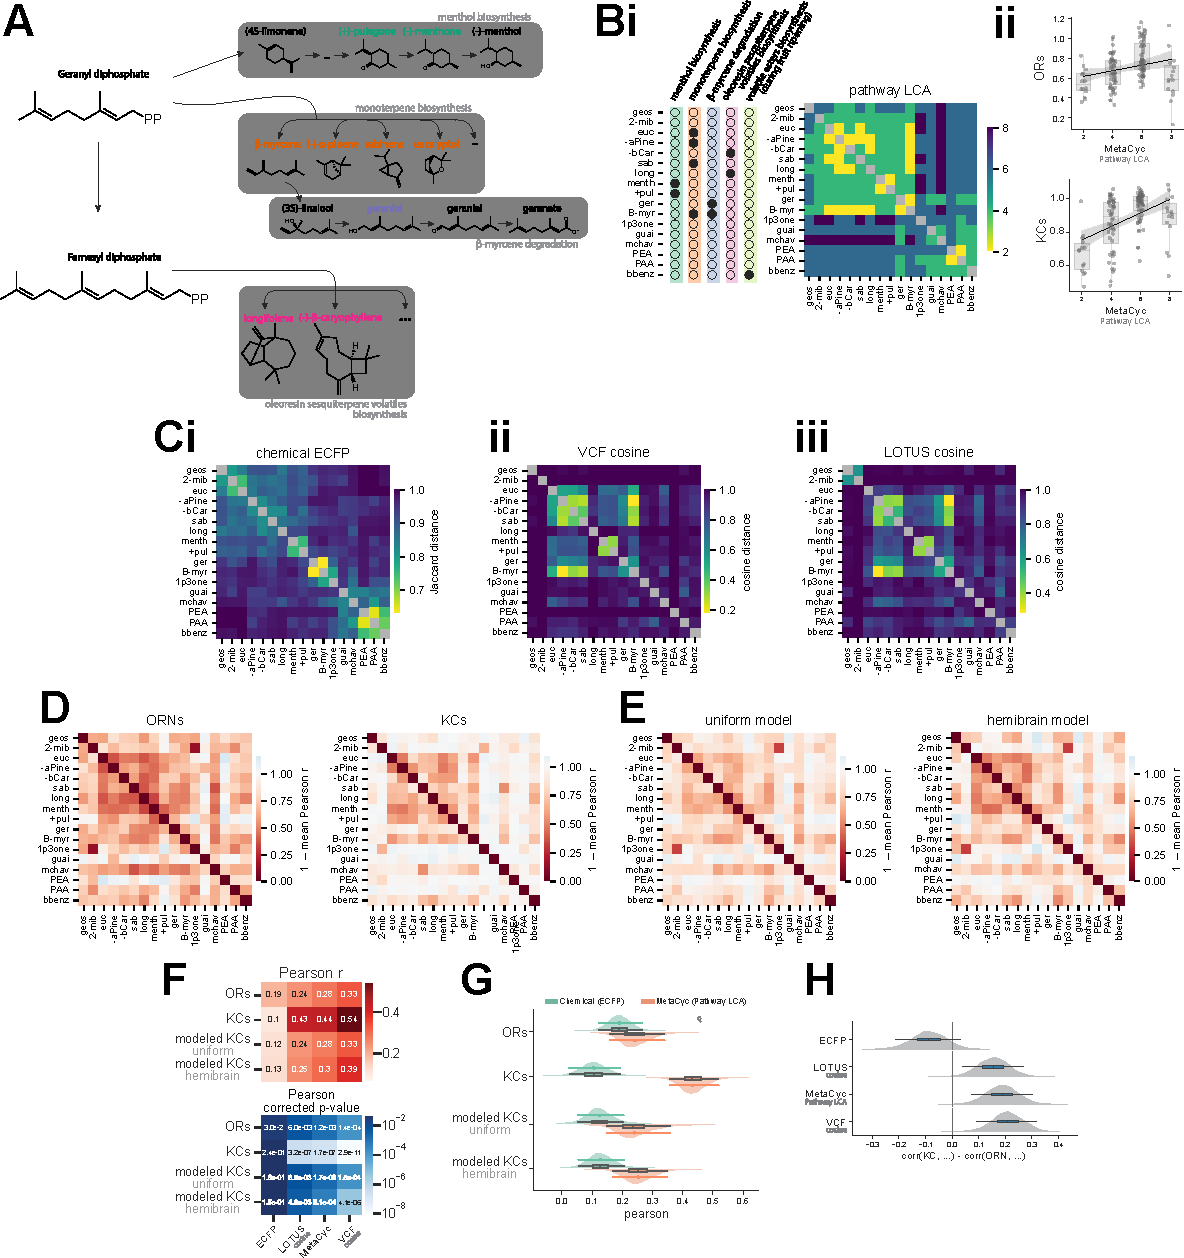
\includegraphics[width=\textwidth]{5}
\mycaptionof{figure}{Odor relationships in KC soma track metabolic and natural source relationships more closely than those in ORN terminals}{%
% TODO reword "All panels", since A doesn't?
All panels show a second 17-odor panel chosen to span a range of known metabolic distances in the MetaCyc database.
All distance matrices show the 17 odors in the same order.
}
\label{fig:5}

% TODO delete?
%Odors are in the same order from B--G.
 
\mysubcaption{A}{%
Example MetaCyc pathways that produce odors in the panel.
Panel compound names are shown in color, non-panel compounds names are shown in black.
Pathways are linked when a product of one is a reactant of the other.
Pathway boundaries are indicated by boxes and correspond to the pathways shown in \textbf{(Bi)}.
Superpathways, which group pathways with common metabolites or which carry out a common biological function, are not shown here but are included as pathway nodes when the network is constructed.
}

% TODO should subfig labelling be bold, both in A) and in A reference in-line below (and throughout)
% (Neuron does not, at least not in Endo2020. they do however have parens around in-line refs)
% our preprint DOES though, and i think i probably prefer it
\mysubcaption{Bi}{%
Metabolic distance between odorants.
Left, filled circles indicate pathway membership of panel compounds in the MetaCyc pathways shown in \textbf{(A)}.
Right, the distance between two compounds within the network of pathways that produce them was computed as the sum of distances from the pathways containing each compound and their lowest common ancestor (pathway LCA distance). %\\
}

% NOTE: currently still need to omit the \\ at end of line above, in order for all this text to fit on one page
% (or at least, without triggering previous page to be blank)

\mysubcaption{Bii}{%
Odor-odor distances in ORN terminals (top) and KC somata (bottom) against metabolic pathway distances as shown in \textbf{(Bi)}.
Each point indicates an odor pair; and boxes indicate medians and IQRs; the line shows a linear fit.
}

\mysubcaption{C}{%
\textbf{i)} Chemical structural distance between odor compounds, computed as the Jaccard distance between binary ECFP6 fingerprint vectors.

\textbf{ii-iii)} Odor-odor distances in natural source spaces, computed as the cosine distance between binary source feature vectors (1 if the compound appears in a given source, 0 if not), using:
\textbf{ii)} The VCF database, where sources are foods.
\textbf{iii)} The LOTUS Natural Products database, where sources are organisms.
}

%
%Ciii) Odor-odor distances in natural source space, computed from the LOTUS Natural Products database of structure-organism pairs (i.e. chemical compounds and the living organisms in which they were found).
%distances were computed as the cosine distance between binary organism feature vectors (1 if the compound was identified in a given organism, 0 if not).

\mysubcaption{D}{%
Odor-odor distances in observed neural representations in ORN terminals (left, $n{=}5$ flies) and KC somata (right, $n{=}20$ flies).
Distances were computed as ($1 - \text{Pearson's } r$) between trial-averaged peak amplitude population responses; distances were then averaged across flies.
}

\mysubcaption{E}{%
Odor-odor distances for simulated KC responses, under two models of PN-KC connectivity: uniform (left), in which each KC draws its inputs independently from a uniform distribution across glomeruli, and hemibrain (right), in which the PN-KC weights are derived from synapse counts in the hemibrain EM dataset.
}

\mysubcaption{F}{%
Pearson's $r$ (top) and their corrected $p$-values (bottom) between odor-odor distances in four neural spaces (observed ORN terminals, observed KC somata, and uniform/hemibrain model KCs) (rows), against chemical structure space (ECFP) and three natural source spaces (LOTUS, MetaCyc, VCF) (columns).
$n{=}136$ odor pairs, two-sided $t$-test, corrected by Benjamini-Hochberg.
}

\mysubcaption{G}{%
Distributions of Pearson's $r$ between odor-odor distances in ORN terminals or KC somata (observed and modeled) (rows) against chemical (ECFP, green) or metabolic (orange, pathway LCA) distances for \num{5000} random subsamples of 80\% of the 136 odor pairs, computed without replacement.
}

\mysubcaption{H}{%
Difference between KC somata and ORN terminals in their Pearson correlation with each reference space $X$ ($r(\text{KC}, X) - r(\text{ORN}, X)$), for chemical (ECFP), metabolic (MetaCyc), and natural source (LOTUS, VCF) distance.
Positive values indicate a stronger correlation in KCs.
Distributions come from \num{5000} subsamples of 80\% of the 136 odor pairs, as in \textbf{(G)}.
}
\end{longcapfigure}
% }

We theorized that the underlying reason for the hyperbolic structure of natural source space (as measured in food sources) is that occurrence of the compounds in food sources is determined by the metabolic pathways that produce them.
To test if the remapping observed in the olfactory pathway is related to their distance in metabolic space, we looked to the MetaCyc database, a highly curated encyclopedia of metabolic pathways from all domains of life, containing over \num{3000} pathways and over \num{20000} chemical compounds\cite{MetaCyc}.
MetaCyc groups chemical reactions and their reactants and products into pathways whose boundaries are defined by coincidence with currency metabolites, regulatory units, and evolutionarily conserved metabolic units.

Using MetaCyc, we identified another panel of odor compounds of varying structural similarity, of which various subgroups of odors were produced by common pathways or in different pathways of varying proximity, such as monoterpene biosynthesis and $\beta$-myrcene degradation (\cref{fig:5:A}).
Chemical structure similarity was calculated as the Tanimoto distance between ECFP6 fingerprints (\cref{fig:5:C}i).
To compute metabolic distance, we constructed a directed graph network in which pathways and their reactants/products were nodes.
First, directed edges were drawn from the reactants of a pathway to the pathway itself, making each reactant a parent node of the pathway node.
Likewise, the same was done with pathways and their products, making each product compound a child node of a pathway node.
Pathways were connected through compound nodes, if a product (child) node of one pathway was also the reactant (parent) node of another pathway.
The distance between two compounds in the pathway network was defined as the sum of the distance from each compound to their lowest common ancestor (LCA) node (\cref{fig:5:Bi}). 

Because these compounds were also found in the VCF database, their distances in food space were also computed.
For this panel, however, distances were not taken from a hyperbolic embedding and were instead computed directly as the cosine distance between binary vectors of compound-food occurrences (\cref{fig:5:C}ii).

Finally, we measured the odor distances in an additional natural product database, LOTUS, which contains \num{750000} structure-organism pairs, whose sources encompass a wider class of organisms than the food-focused VCF database (\cref{fig:5:C}iii)\cite{LOTUS}.
Responses to this odor panel were collected from ORN terminals and KC soma, and we once again used our ORN data as input to construct model KC responses for the same uniform and hemibrain variants used previously.
Odor-odor distance matrices were computed using 1 - Pearson correlation between response vectors of each odor, for our ORN and KC measurements (\cref{fig:5:D}) and for the outputs of our two models (\cref{fig:5:E}).

We found that the nature of the olfactory pathway remapping observed using the previous odor panel chosen to widely sample ORN odor space was also observed in this second odor panel which was chosen to contain a range of measurable metabolic distances (\hyperref[fig:5:Bi]{\cref*{fig:5}B}).
Metabolic pathway distance, as determined by total distance to a LCA in the directed pathway network, was a stronger predictor of odor-odor dissimilarity in the KCs ($\rho {=}0.44$, $p{=}\num{1.7e-7}$) than the ORN terminals ($\rho {=}0.12$, $p{=}\num{2.4e-3}$).
Chemical similarity was also more strongly reflected by the ORNs (Pearson correlation, $\rho {=}0.19$, $p{=}\num{3.0e-2}$) than KCs ($\rho {=}0.1$, $p{=}\num{2.4e-1}$).
KC odor distances were not significantly correlated with chemical (ECFP) distances (\cref{fig:5:F}).
In addition to being more strongly correlated with metabolic distance, KC distances were also more strongly correlated than ORNs to relationships in the LOTUS (ORN $\rho {=}0.24$, $p{=}\num{4.0e-3}$; KC $\rho {=}0.43$, $p{=}\num{3.2e-7}$) and VCF datasets (ORN $\rho {=}0.33$, $p{=}\num{1.4e-4}$; KC $\rho {=}0.54$, $p{=}\num{2.9e-11}$).

To determine whether this relationship was driven by a small fraction of odor pairs, we resampled 80\% of the odor pair dissimilarities without replacement \num{50000} times.
For each resampling iteration, we computed the correlation between the various neural distances (both observed and modeled) and the chemical and pathway distances (\cref{fig:5:G}).
Odor distances in KC space were significantly more correlated with metabolic pathway distances than with chemical structure distances (note non-overlapping chemical and pathway distributions in \cref{fig:5:G}).
While both ORN and KC spaces were somewhat positively correlated with both metabolic space and chemical space, KCs were significantly more correlated with pathway distance than ORNs, and the correlation with metabolic space was significantly greater than with chemical space for observed KCs only.
Both observed and modeled KC distances were less correlated with chemical space than ORNs were, though the difference was not significant.
Interestingly, while the modeled results effectively capture the weakened relationship of the KCs to chemical structure, neither model predicted KC responses that align odor distances with metabolic space to the extent observed in the KCs.


\subsection{Odor relationships are restructured across successive stages of olfactory processing}

% Figure 6
% {
\begin{longcapfigure}
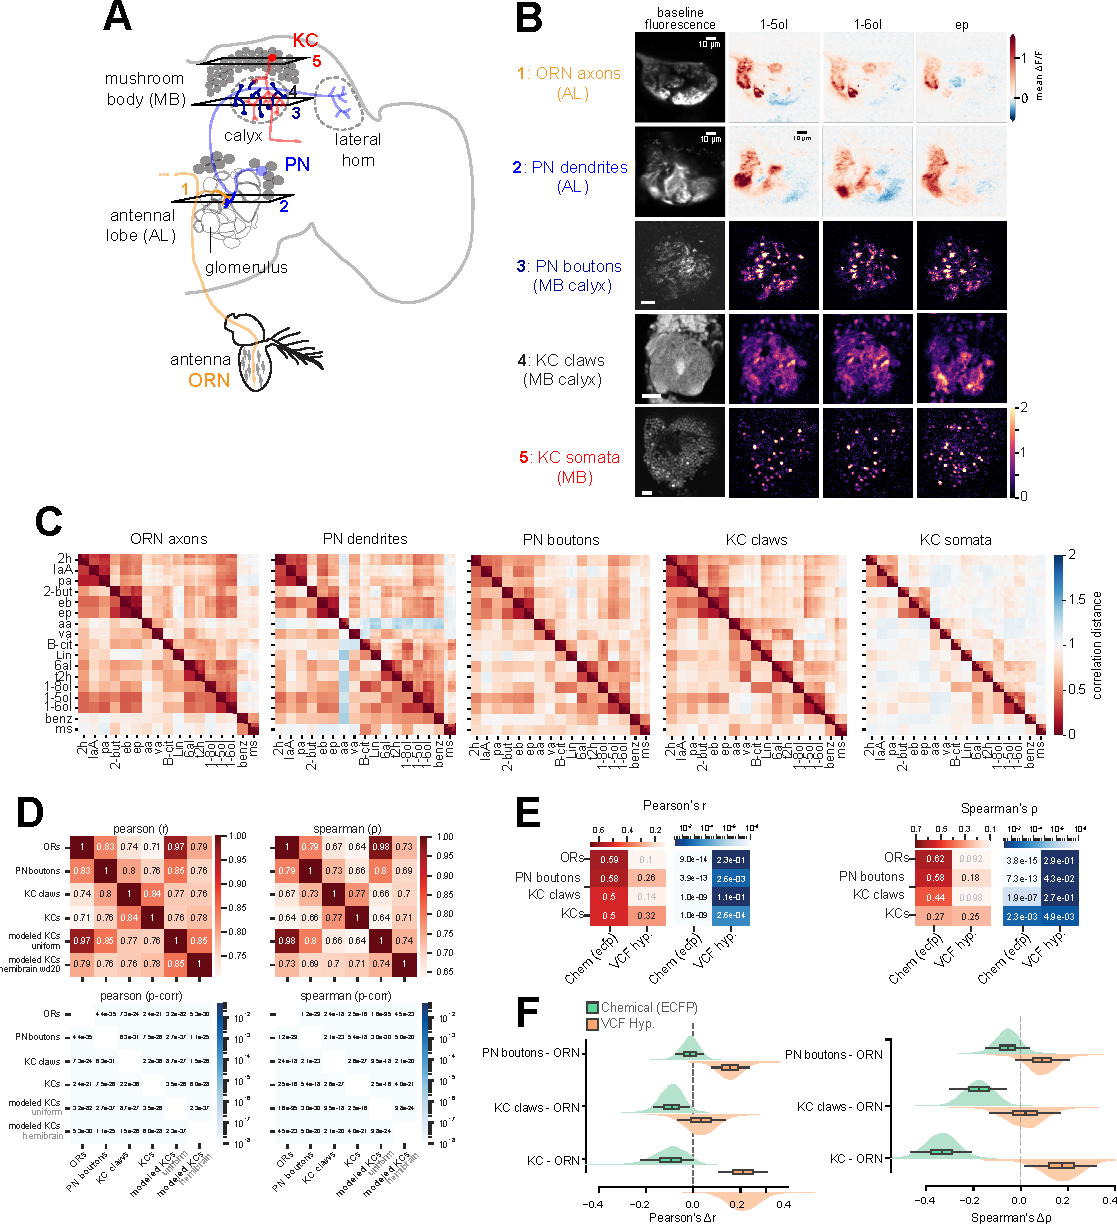
\includegraphics[width=\textwidth]{6}
\mycaptionof{figure}{Reformatting of odor representations across four stages of olfactory processing}{}
\label{fig:6}

\mysubcaption{A}{%
Anatomical schematic of fly olfactory circuit.
ORN axon terminals are organized in a stereotyped glomerular map in the AL.
Each uniglomerular PN has dendrites in a single AL glomerulus and projects to the calyx of the MB, where its axonal arbor terminates in multiple boutons that each synapse with KC input claws.
}

% TODO TODO TODO update text. it's only mean, not peak, for at least ORN and PN dendrites, right?
\mysubcaption{B}{%
Representative baseline fluorescence and peak \DeltaFOverF\, heatmaps of odor-evoked calcium signals in ORN axon terminals, PN dendrites, PN boutons, KC claws, and KC somata to 1-pentanol, 1-hexanol, and ethyl propionate.
KC data are reproduced from \cref{fig:1}.
Scale bar, \qty{10}{\micro\metre}.\\
% TODO TODO just refer to table for all these full genotypes?
Genotypes:
ORN axons were imaged in pebbled-Gal4/+; +; 20xUAS-IVS-syn21-opGCaMP6f-p10/+.
PN dendrites were imaged in +; GH146-Gal4/+; 20xUAS-IVS-syn21-opGCaMP6f-p10/+.
PN boutons were imaged in GH146-Gal4/20xUAS-IVS-jGCaMP8m (II).
% TODO TODO TODO did remy actually use a jGCaMP8m on both II and III (as was indicated in my version of her table), or was it always on II, like prat mentioned?
% (assuming below is her original text (and is correct), her table was wrong)
KC claws were imaged in 20xUAS-IVS-jGCaMP8m/+ (II); OK107-Gal4/+ (IV).
KC soma were imaged in 20xUAS-nls-OpGCaMP6s-p10/+ (III); OK107-Gal4/+ (IV).
}

\mysubcaption{C}{%
Matrix of mean pairwise correlation distances (averaged across flies) of trial-averaged odor representations in ORN axons ($n{=}9$ flies), PN dendrites ($n{=}6$ flies), PN boutons ($n{=}6$ flies), and KC somata ($n{=}4{-}18$ flies; see \cref{fig:s7}) to a panel of 17 odors.
Odors are displayed in the same order in each matrix according to the clustering of their representations in KC representational space.
}

\mysubcaption{D}{%
Odor representations are correlated across stages of the olfactory pathway.
Top: Pearson's $r$ (left) and Spearman's $\rho$ (right) between the across-fly mean odor-odor dissimilarity matrices \textbf{(C)} of ORN terminals, PN boutons, KC claws, and KC soma, and two model KC populations (uniform and hemibrain).
% TODO be consistent about "corrected by B-H" vs "B-H FDR-corrected"?
Correlations between each of the neural representation spaces were computed over the $n{=}136$ odor pair combinations (17 odors).
Bottom: corresponding two-sided $p$-values, Benjamini-Hochberg FDR-corrected.
}

\mysubcaption{E}{%
Comparison of each stage's odor representation to two reference spaces: chemical structure space computed from extended-connectivity fingerprints (``Chem (ECFP)'') and the natural source space in a hyperbolic embedding (``VCF hyp.'').
Pearson's $r$ (left block) and Spearman's $\rho$ (right block) between the mean odor-odor distances in each neural space and the odor-odor distances in each reference space (red) with Benjamini-Hochberg FDR-corrected two-sided $p$-values (blue); $n{=}136$ odor pairs, gray values indicate $p\,{\geq}\,0.05$.
}

\mysubcaption{F}{%
Bootstrap distributions of the change in reference-space correlation relative to ORN axons at successive downstream stages of the olfactory pathway.
Left: Pearson's $\Delta{}r = r(\text{olfactory stage}, \text{space}) - r(\text{ORN axons}, \text{space})$, right: Spearman's $\Delta\rho$, obtained by resampling the 136 odor pairs with replacement (\num{5000} iterations).
Boxes show mean and interquartile range; whiskers, 90\% CI.
The dashed line indicates no difference from ORN axons.
Green, chemical (ECFP) reference space; orange, natural source reference space (embedded VCF distances).
Values right of zero indicate closer correspondence to that reference space than ORN axons; left, weaker.
}
\end{longcapfigure}
% }

To better understand how representations of odor are reformatted from the periphery to the MB, we used functional imaging to measure odor-evoked patterns of activity at each successive stage of processing in the olfactory circuit.
% TODO this correct citation?
While delivering odors to the antennae of the fly, we volumetrically imaged from all ORN axon terminals (labeled by the pebbled-Gal4 driver) or from \textasciitilde70\% of PN dendrites (labeled by the GH146-Gal4 driver) in the antennal lobe\cite{Zocchi2022}, where the neurites from these cell populations are stereotypically organized into glomerular compartments with characteristic size and position (\cref{fig:6:A}-\subref{fig:6:B}).
% TODO TODO delete part about Hallem ORs only being about half input? really relevant still?
Population imaging from the terminals of all ORN classes allowed assessment of odor relationships in the complete OR input space to the olfactory system, whereas the Hallem dataset measures the tuning of only approximately half of all fly ORs. % (Supplemental Figure ???).
Regions of interest corresponding to individual glomeruli were manually segmented from movies of odor responses in ORN axon or PN dendrites and their odor response profiles extracted.
To evaluate patterns of odor-evoked PN output, we volumetrically imaged from the axonal boutons of \textasciitilde70\% of PNs (labeled by the GH146-Gal4 driver) in the calyx of the MB, where they synapse onto the sites of KC input (claws).
ROIs corresponding to PN boutons were automatically segmented using Suite2P; visual inspection confirmed that >95\% of ROIs reliably corresponded to single PN boutons.
To measure KC input, we imaged KC claws (labeled by the OK107-Gal4 driver) in the calyx volumetrically and extracted ROIs using Suite2p.
For each stage, odor-by-odor distance matrices were computed per fly using correlation distance (1 - Pearson's $r$) between odor-evoked, trial-averaged population response vectors, then averaged across flies (\cref{fig:6:C}).
Odor relationships were invariant across the brains of different individuals at each of these earlier stages of olfactory processing (\crefwithbackref{fig:s6:A}).

We previously showed that the ORN-to-KC restructuring aligns KC odor distances with odor relationships based on compound distributions in food sources, while decreasing the extent to which they reflect chemical structure similarities.
We extended our comparisons to PN boutons and KC claws.

Comparing the correlation distances between odor representations in each layer of the olfactory circuit, we found that odor relationships were correlated between all stages of the pathway (\cref{fig:6:D}), but their correspondence with the ORN input declined at each successive stage.
Odor relationships in the ORN terminals were most strongly reflected in the PN boutons, and most weakly reflected in the KC somata.
Across the pathway, the relative ranking of odor-odor distances in each layer was only partially maintained (ORN terminals versus KC somata, $\rho {=} 0.64$, $p{=}\num{2.5e-16}$), indicating that odor relationships are transformed beyond a simple linear scaling between layers (\cref{fig:6:D}, right column). 

We previously observed that ORN representations reflect chemical structure to a greater extent than KC representations do, but KC soma representations captured natural source relationships that were not reflected by ORNs (\cref{fig:4:D}).
Extending this comparison to the PN boutons and KC claws revealed that odor relationships at every stage are significantly correlated with chemical structure relationships, but this correlation weakened at each stage of the pathway, and did so smoothly-- this was most noticeable in the rank order comparison ($\rho {=}$0.62, 0.58, 0.44, and 0.27 for ORNs, PN boutons, KC claws, and KC soma, respectively) (\cref{fig:6:E}, right).
A bootstrap analysis confirmed that the largest drop in correlation with chemical structure, relative to the ORNs, occurred in the KC somata ($\Delta \rho {=} -0.34$, 90\% CI [-0.45, -0.24]).
A smaller drop occurred in KC claws ($\Delta \rho {=} -0.18$, 90\% CI [-0.28, -0.08], while the change in PN boutons ($\Delta \rho {=} -0.04$, 90\% CI [-0.12, 0.03]) was not significant (\cref{fig:6:F}).

% TODO TODO check these claude corrections
%Natural source relationships were not reflected in the ORNs or KC claws ($\rho {=}0.090$, $p{=}0.27$), and reflected most strongly in the KC soma ($\rho {=}0.62$, $p{=}\num{2.3e-3}$).
Natural source relationships were not reflected in the ORNs or KC claws ($\rho {=}0.090$, $p{=}0.27$), and reflected most strongly in the KC soma ($\rho {=}0.25$, $p{=}\num{4.9e-3}$).
%Interestingly, the PN bouton representations also reflected natural source relationships, though to a lesser extent ($\rho {=}0.18$, $p{=}\num{7.3e-13}$).
Interestingly, the PN bouton representations also reflected natural source relationships, though to a lesser extent ($\rho {=}0.18$, $p{=}0.043$).
% TODO TODO TODO check claude output. r supposed \rho?
%Bootstrap estimates of the change relative to ORNs were positive for KC somata ($\Delta r = +0.21$, 90\% CI \numrange{0.11}{0.32}; $\Delta \rho {=} +0.16$, 90\% CI \numrange{0.04}{0.28}) and for PN boutons using rank correlations ($\Delta r = +0.16$, 90\% CI \numrange{0.08}{0.24}).
Bootstrap estimates of the change relative to ORNs were positive for KC somata ($\Delta r = +0.21$, 90\% CI \numrange{0.11}{0.32}; $\Delta \rho {=} +0.16$, 90\% CI \numrange{0.04}{0.28}) and for PN boutons using rank correlations ($\Delta r = +0.16$, 90\% CI \numrange{0.08}{0.24}).
KC claws did not shift meaningfully in their natural source correlation from the ORNs. 

% old text, when fig 6 was fig 5
\iffalse
To better understand how representations of odor are reformatted from the periphery to the MB, we used functional imaging to measure odor-evoked patterns of activity at each successive stage of processing in the olfactory circuit.
While delivering odors to the antennae of the fly, we volumetrically imaged from all ORN axon terminals (labeled by the pebbled-Gal4 driver) or from \textasciitilde70\% of PN dendrites (labeled by the GH146-Gal4 driver) in the antennal lobe\cite{Zocchi2022}, where the neurites from these cell populations are stereotypically organized into glomerular compartments with characteristic size and position (\crefwithbackref{fig:5}A-B).
% TODO delete. that ref is surely bad too
%Population imaging from the terminals of all ORN classes allowed odor relationships to be assessed in the complete OR input space to the olfactory system, whereas the Hallem dataset measures the tuning of only approximately half of all fly ORs (Supplemental \cref{fig:s4}B).
ROIs corresponding to individual glomeruli were manually segmented from movies of odor responses in ORN axon or PN dendrites and their odor response profiles extracted.
To evaluate patterns of odor-evoked PN output, we volumetrically imaged from the axonal boutons of \textasciitilde70\% of PNs (labeled by the GH146-Gal4 driver) in the calyx of the MB, where they synapse onto the sites of KC input (claws) (\cref{fig:5}A,B).
ROIs corresponding to PN boutons were automatically segmented using Suite2p; visual inspection confirmed that >95\% of ROIs reliably corresponded to single PN boutons.
Odor relationships were invariant across the brains of different individuals at each of these earlier stages of olfactory processing (\cref{fig:s4}A), consistent with the stereotyped connectivity of the antennal lobe.

% TODO TODO update supplemental fig refs
Comparing the pairwise correlation distances between odor representations in each layer of the olfactory circuit, odor representations were progressively decorrelated at each feedforward stage of processing (\cref{fig:5}C), with the mean and median odor-odor correlation becoming systematically lower in each successive layer (\cref{fig:s4}D).
The largest decorrelation occurred between PN boutons and KC somata, consistent with the divergent expansion of the circuit at this synaptic step.
However, the rank order of odor-odor distances was not maintained across layers (ORN terminals versus KC somata, Spearman's $\rho{=}0.48$), indicating that odor relationships are transformed beyond a simple linear scaling between layers.
For comparison, in a model that assumes unstructured PN input to KCs and uniform inhibition in the AL and MB (``uniform''), the Spearman's correlation between odor relationships in the input OR layer and in modeled KCs is $\rho{=}0.83$.
Furthermore, whereas the relative levels of odor-evoked activity in PNs dendrites or boutons was well-predicted by levels of overall ORN input to the circuit, odor evoked KC response rates (and mean activity) were comparatively less well-predicted (\cref{fig:5}D, \cref{fig:s4}Ci-iv, and data not shown).
These observations all point towards a non-linear reformatting of odors in the MB representational space that alters the rank ordering of odor relationships compared to earlier stages of coding.

We examined odor relationships at each step of processing using hierarchical clustering of odor representations in each neural population, in order to better understand the origins of odor relationships in MB coding space.
For instance, one of the strongest odor clusters at the level of input representations – 2-heptanone, isoamyl acetate, and pentyl acetate – was maintained in each subsequent stage of processing through to the KCs (\cref{fig:5}C,E).
These odors share a high degree of chemical similarity as well as co-occurrence in natural sources, which may explain their robust grouping.
However, other odor representations that were similarly well correlated and clustered in OR space (e.g., 1-pentanol and 2-butanone) were selectively decorrelated in KC coding space, with each odor becoming reassigned to distinct, non-overlapping groups of odors in KC coding space (\cref{fig:5}C,E).
Additionally, the representations for some odor pairs were observed to become reliably more similar at later stages of olfactory processing.
For instance, the pairwise correlation distances between 1-pentanol and 1-hexanol was actually shorter in KC coding space as compared to in ORN axon, PN dendrite, or PN bouton coding space.

Typically, these transformations in the representational geometry among odors occur progressively at each successive stage of processing, with the largest change occurring between PN boutons and KC somata (\cref{fig:5}C).
However, we observed significant reorganization of odor representations even between the inputs and outputs of the same cell population, PNs; odor relationships encoded in PNs boutons better reflect odor relationships in KC coding space compared to PN dendrites (\cref{fig:5}C,E).
The nonlinear reformatting of odor relationships across successive stages of olfactory coding indicates that prevailing models of olfactory networks that assume global or uniform processing across neurons are incomplete, and additional sources of structure exist in the fly olfactory circuit that mediate non-uniform interactions between olfactory coding units (e.g., neurons or glomeruli).
\fi

\section{Discussion}
We show that representations of odor are structured and invariant across MBs in individual flies, and that the structure of MB odor coding space is only partially predicted by models that assume that olfactory inputs (glomeruli) wire randomly to KCs.
The latter is true even after adjusting the MB model to incorporate PN-KC connections from the hemibrain connectome, which contains the documented over- and under-convergence of specific sets of glomeruli onto KCs (`hemibrain' model) (\cref{fig:s4:E})\cite{CommunityPNs}.
Thus, certain assumptions of olfactory system architecture – for instance, of uniform strengths of unitary feedforward synapses, uniform spiking thresholds, or nonselective, global inhibition in the AL or MB – are likely oversimplifications, motivating a search for source(s) of structured interactions between glomeruli or neurons in the olfactory circuit.
% for reference, other versions of first paragraph that mention hemidraw:
% preprint:
\iffalse
We show that representations of odor are structured and invariant across MBs in individual flies, and that the structure of MB odor coding space is only partially predicted by models that assume random sampling of olfactory glomerular inputs by KCs.
The latter is true even after adjusting the MB model to account for the over- or under-representation of PN boutons from specific glomeruli (“hemidraw” model) or the amount of over- and under-convergence of PN inputs from specific sets of glomeruli onto KCs (“hemibrain” model).
Thus, certain assumptions of olfactory system architecture – for instance, of uniform strengths of unitary feedforward synapses, uniform spiking thresholds, or nonselective, global inhibition in the AL or MB – are likely oversimplifications, motivating a search for source(s) of structured interactions between glomeruli or neurons in the olfactory circuit.
\fi
% working copy as of 2026-10-07:
\iffalse
We show that representations of odor are structured and invariant across MBs in individual flies, and that the structure of MB odor coding space is only partially predicted by models that assume that olfactory inputs (glomeruli) wire randomly to KCs.
The latter is true even when predicted KC responses were adjusted to reflect the over- or under-representation of PN boutons from specific glomeruli (“hemidraw” model) or the amount of over- and under-convergence of PN inputs from specific sets of glomeruli onto KCs (“hemibrain” model).
Thus, certain assumptions of olfactory system architecture – for instance, of uniform strengths of unitary feedforward synapses, uniform spiking thresholds, or nonselective, global inhibition in the AL or MB – are likely oversimplifications, motivating a search for the source(s) of structured interactions between glomeruli or neurons in the olfactory circuit. 
\fi

We demonstrate a significant transformation of the fly olfactory code between the periphery and the MB, in which the encoding of odors by ORs better reflects the chemical relationships between odors and the encoding of odors in the MB better reflects the distributions of odors across behaviorally relevant natural sources.
That representations at the olfactory periphery better capture odor relationships in terms of their chemical or molecular properties is perhaps unsurprising, since odor-OR interactions are governed by the structural features of the odor.
The reorganization of MB odor representations to better correlate with the relationships of these odors in natural source space may reflect the progressive transformation of odor representations in the olfactory network to encode latent variables that relate more directly to behavioral value or perception.

Odor distances in the hyperbolic embedding of natural odor mixtures reflect correlations between volatiles in the headspace profiles across natural sources that arise from conserved metabolic pathways\cite{HyperbolicOdors}.
The transformation of odor representations in the MB is predicted to facilitate the perceptual compression of odors that have shorter metabolic tree distances in the hierarchical organization of natural odor mixtures relative to their chemical similarity.
Consistent  with this idea, a recent study reports that distances between odors in a neural network embedding trained on human olfactory perceptual labels are correlated with the metabolic distance between odors in experimentally elucidated biochemical pathways\cite{MetabolicActivityRepresentations}.

The specific structure of odor relationships was largely invariant across individual brains at each stage of olfactory processing (\cref{fig:2}), even in the MB where PN boutons connect probabilistically with KCs.
An important open question is the extent to which the invariance of MB representational space may arise from genetically specified developmental processes (sculpted by evolution) or from activity-dependent processes that reflect shared olfactory experience\cite{CorticalOdorSpace}.
Unlike their mammalian analogues in piriform cortex, KCs are not strongly connected through recurrent excitation, although the degree to which PN-KC synapses or APL-KC synapses may be regulated by experience is not well understood.
We note that the structure of PN overconvergence onto KCs bears significant similarity to the structure of PN input to third order olfactory neurons in the lateral horn (LH) (\cref{fig:s4:E}).
LH neurons are stereotyped in their anatomical connectivity and odor tuning and are believed to mediate innate olfactory behaviors.
The similarity in PN input structure between the MB and LH points to the likely ethological significance of these over-represented glomerular combinations.
It also raises the possibility that the LH may have additional roles in shaping odor representations in the MB.
For instance, neurons downstream of the LH send centrifugal input to the MB calyx\cite{LHNsToMBWithSplitsAndActivation} which could contribute to the remapping of odor representations in PN boutons.
Other possible sources of structure in the circuit are selective inhibition from the APL or MB-C1 neurons in the calyx, or non-uniform PN-KC synaptic weights.
Understanding the specific circuit mechanisms that shape the reorganization of odor representations in the MB will be important for understanding how odor relationships in natural sources become reflected in the olfactory code.

Theoretical studies of divergent expansive cerebellum-like circuits such as the MB emphasize the computational benefits of random networks for maximizing coding capacity and promoting the separability and discriminability of representations.
However, structured networks can correlate odor representations and promote generalization of odors along important directions of odor space, for instance, related to the relationships of odorant molecules in behaviorally salient natural odor sources.
Our results suggest a revision of classic formulations of cerebellar-like network architectures is warranted at least in some systems: the MB may trade-off the capacity to maximally decorrelate activity patterns in parts of representational space for an increase in coding capacity and robustness in a part of representational space of particular ethological significance\cite{StructuredCerebellarConns}.
The recoding of odors in the MB to reflect relationships in natural sources would predict greater generalization to odors with similar distributions in the environment, facilitating the decoding of natural source identity in noisy or ambiguous situations.

% TODO delete. don't think i care about fig 7 (unless it makes it easier to say this chapter is as submitted / in prep...)
% (also not currently planning to show the one supplemental fig for dynamics (S7))
\iffalse
% TODO add text that actually refers to this figure
% Figure 7
% {
\begin{longcapfigure}
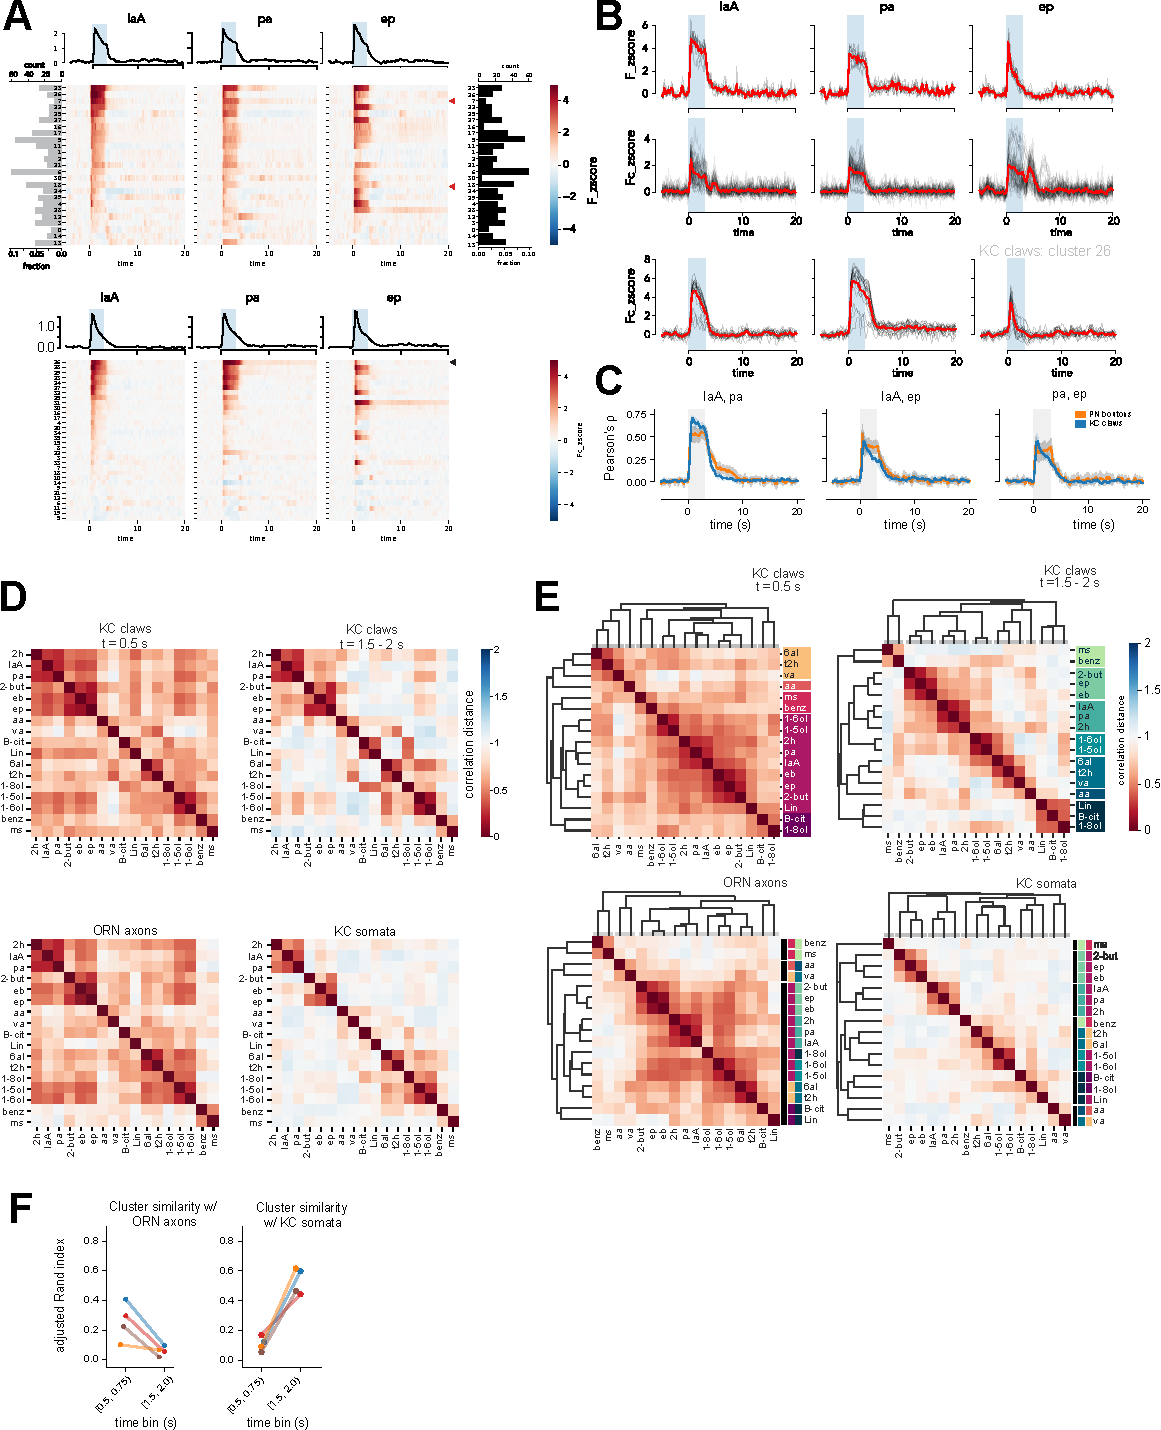
\includegraphics[width=\textwidth]{7}
\mycaptionof{figure}{TODO TODO fig 7 DESCRIPTION}{%
% TODO code formatting for rastermap?
A) Odor-evoked responses of PN boutons (top) and KC claws (bottom) to odors isoamyl acetate (IaA), pentyl acetate (PA), and ethyl propionate (ep);  Each row is one cluster's trial-averaged response; clusters were generated using `rastermap`, then sorted to group similar IaA response profiles; color, z-scored fluorescence. Marginal bars, number and fraction of boutons/claws per cluster; Marginal line plot, mean z-scored fluorescence across ROIs; blue shading, \qty{3}{\second} odor delivery.

B) Individual traces (gray) and cluster mean (red) for representative clusters: PN boutons cluster 7 (top) and 18 (middle), KC claws cluster 26 (bottom).
Blue shading, odor delivery.

C) Time course of pairwise correlation between odor representations for three odor pairs, in PN boutons (orange) and KC claws (blue). Correlation rises during odor delivery and decays over the following \textasciitilde\qty{10}{\second} in both boutons and claws.
gray shading, odor delivery.

D) Odor–odor correlation distance matrices for 17 odors, computed from KC claw responses in an early [0.5, 0.75)\,\unit{\second} and a late [1.5, 2.0)\,\unit{\second} time window, shown above ORN axon and KC somata matrices for reference.
Odors in the same order in every panel.

E) The same four matrices, reordered by hierarchical clustering (average linkage, number of clusters per matrix chosen by silhouette score analysis, shown with optimal leaf ordering. Color strips indicate cluster  cluster assignment).
5 clusters for the early KC claw response, 7 for late KC claw response, 3 clusters for ORNs, 6 clusters for KC soma.

F) Adjusted Rand index between KC claw odor clusters and those of ORN axons (left) or KC somata (right), in the early and late time windows. Each line is one fly ($n{=}4$). KC claw clustering resembles ORN axons early and KC somata late, with all 4 flies shifting in the same direction in both comparisons.
}
\label{fig:7}
\end{longcapfigure}
% }
\fi
% end part to delete (fig 7)

\processdelayedfloats

\section{Methods}
% TODO rename?
\subsection{Experimental model}
\textit{Drosophila melanogaster} were raised on a 12:12 light:dark cycle at \qtyrange{23}{25}{\degreeCelsius} and \qtyrange{60}{70}{\percent} relative humidity on cornmeal/molasses food containing: water (\qty{17.8}{\litre}), agar (\qty{136}{\gram}), cornmeal (\qty{1335.4}{\gram}), yeast (\qty{540}{\gram}), sucrose (\qty{320}{\gram}), molasses (\qty{1.64}{\litre}), \ce{CaCl2} (\qty{12.5}{\gram}), sodium tartrate (\qty{150}{\gram}), Tegosept (\qty{18.45}{\gram}), 95\% ethanol (\qty{153.3}{\milli\litre}) and propionic acid (\qty{91.5}{\milli\litre}).
All experiments were performed in female flies aged \numrange{3}{10} days post-eclosion.

Unless otherwise noted, the fly lines in this study were acquired from the Bloomington Drosophila Stock Center (BDSC) and have been previously characterized as discussed below.
1) pebbled-Gal4 (X), targeting all ORNs (\bdsc{80570})\cite{pebbled};
2) GH146-Gal4 (II), targeting \textasciitilde70\% of PNs (\bdsc{30026})\cite{GH146};
3) OK107-Gal4 (IV), targeting all KCs (\bdsc{854})\cite{OK107}.

We utilized three genetically encoded calcium indicators to record neuronal activity within respective neuropil compartments, all of which are expressed in a Gal4-dependent manner:
1) 20xUAS-IVS-jGCaMP8m (II) (\bdsc{92591})\cite{jGCaMP8};
2) 20xUAS-nls-OpGCaMP6s-p10 (III) was provided by H. Chiu and D.J. Anderson (Caltech, Pasadena, CA) and expresses nuclear-localized OpGCaMP6s\cite{CodonOptimizedGCaMP6s};
% TODO also cite some anderson paper for codon optimized version of this one?
3) 20xUAS-IVS-syn21-OpGCaMP6f-p10 (III), provided by H. Chiu and D.J. Anderson (Caltech, Pasadena, CA)\cite{Gen6GCaMPs}.
Indicator lines (2) and (3) express codon-optimized versions of their respective GCaMP.

To enhance response robustness and minimize anomalies caused by inbreeding or genetic bottlenecks, 20xUAS-IVS-syn21-OpGCaMP6f-p10 (III) was back-crossed into our internally-generated wild-type strain for six generations.
The wild-type strain (referred to as 6x) was produced by back-crossing w1118[iso31] and Canton-S (selected for white eyes) for six generations (by Jaison Jiro Omoto).
For pebbled-Gal4 and GH146-Gal4, only wild-type chromosomes from original stocks were replaced with those from the 6x strain.

Full genotypes and sample sizes for each dataset are in Supplemental \Crefwithbackref{table:s1}.

% TODO TODO maybe just comment all this if i don't get something similar from remy on KC side of things?
% TODO TODO TODO and were remy's PN flies actually included in this? maybe not, esp if not using my genetics...
%\paragraph{ORN \& PN Rearing}
\paragraph{Rearing of flies for ORN \& PN dendrite imaging}
% TODO add sentence saying this is for all but the KC flies? remove paragraph heading? (it's also probably not remy's PN axon flies)
Fly crosses were set up between \numrange{8}{10} males and \numrange{25}{30} virgin females in bottles and flipped every \numrange{2}{3} days to ensure progeny rearing at low density.
% this has now been merged into ranges describing all flies
%Bottles were placed in an incubator at 23°C and \textasciitilde60\% humidity on a 12h:12h light:dark cycle.
Progeny were collected from ZT2 to ZT6, post lights-on, and sorted on a cold-plate to isolate females of the desired genotypes.
Sorted progeny were then placed into vials at low density (\numrange{5}{8} flies per vial) and returned to incubators under identical conditions of light, temperature, and humidity.
Progeny collection from each bottle occurred only during the first three days following initial eclosion.
Additionally, each cross was utilized to establish only three subsequent bottles before being discarded.

\subsection{Odor stimuli}
% TODO TODO TODO update reference, first of all this is showing as 56. in list, and it's not referring to a paper that has these methods. i assume we want to refer to dhruv's paper?
Odors were delivered essentially as previously described\cite{HongWilson2015}.
% TODO also mention it was humidified?
A custom-built multi-channel olfactometer delivered a constant \qty{2}{\litre\per\minute} stream of charcoal-filtered air.
A 3-way solenoid valve directed \qty{200}{\milli\litre\per\minute} of this flow either through a \qty{20}{\milli\litre} glass vial containing \qty{2}{\milli\litre} of odor solution (valve open) or an equivalent vial containing \qty{2}{\milli\litre} of the solvent.
Air flow was controlled using mass flow controllers (MC series, Alicat Scientific, Tucson, AZ).
The \qty{200}{\milli\litre\per\minute} control or odor streams were carried by tubing of matched lengths and rejoined the carrier stream at the same point along the carrier tube, approximately \qty{10}{\centi\metre} from the fly.
The terminal end of the carrier tube had an inner diameter \textasciitilde\qty{8}{\milli\metre} and was \textasciitilde\qty{1}{\centi\metre} away from the fly.
Odor concentrations refer to the v/v dilution factor of the odor solution in the vial.
The concentration of odor in the headspace is further diluted 10-fold in air prior to reaching the fly.
Unless otherwise indicated, all odors in this study were presented from a $10^{-3}$ (0.1\%) dilution in paraffin oil (J.T. Baker, VWR \#JTS894), with the exception of movies collected from one fly, in which odors were diluted to $10^{-2}$ (1\%).

\subsection{Two-photon calcium imaging}
Volumetric, in vivo functional calcium imaging was performed essentially as previously described\cite{HongWilson2015,Zocchi2022}.
After a brief period of cold anesthesia (<\qty{20}{\second}), the fly was head-fixed, and the cuticle, fat, and air sacs were removed to expose the brain region of interest.
Two-photon GCaMP6f or GCaMP8m fluorescence was excited with \qty{925}{\nano\metre} light from a Mai Tai DeepSee laser (Spectra-Physics, Santa Clara, CA).
Images were acquired with an Olympus 20X/1.0 numerical aperture objective (XLUMPLFLN20XW) driven by a piezo motor that enabled fast-\textit{z} scanning, and the collection filter was centered at \qty{525}{\nano\metre} with a \qty{50}{\nano\metre} bandwidth.
Experiments were conducted at room temperature (\textasciitilde\qty{22}{\degreeCelsius}).
% TODO want to change any formatting of concentrations / chemical names here?
% TODO formatting of pH?
The brain was constantly perfused by gravity flow with saline containing (in \unit{\milli\molar}): 103 NaCl, 3 KCl, 5 N-Tris(hydroxymethyl)methyl-2-aminoethane-sulfonic acid, 8 trehalose, 10 glucose, 26 \ce{NaHCO3}, 1 \ce{NaH2PO4}, 1.5 \ce{CaCl2}, and 4 \ce{MgCl2} (pH 7.3, osmolarity adjusted to \qtyrange{270}{275}{\milli\osmole}).
The saline was bubbled with 95\% \ce{O2} / 5\% \ce{CO2} and circulated in the bath at \textasciitilde\qtyrange{2}{3}{\milli\litre\per\minute}.

\subsubsection{AL imaging}
Flies were head-fixed with the dorsal surface of the head approximately parallel to
the imaging plane; the dorsal cuticle was removed, and the antennal lobes were exposed.
The antennae were snugly secured below the imaging chamber, keeping them dry and responsive to odors.
ORN axon terminals and PN dendrites were imaged with a galvo-galvo scanning system (Thorlabs Bergamo).
% TODO TODO update!!! was it all 9-10 planes spaced 10um apart?
Flies were imaged from the dorsal side, with \numrange{9}{10} planes spaced \qty{10}{\micro\metre} apart.
The number of planes and the depth of the first imaging plane were chosen with the goal of capturing signal from all glomeruli.
Images were acquired at a resolution of 192x192 pixels, with typical fields-of-view (FOV) of \textasciitilde\qtyrange{90}{100}{\micro\metre\squared} and volumetric sampling rates of \textasciitilde\qty{1}{\hertz} through the antennal lobe.
For ORN axon and PN dendrite experiments, odors were presented in a pseudorandom order, with the three trials of each odor being presented contiguously.
%Trials consisted of a 7s baseline recording, the odor pulse (2s for ORN experiments and 3s for PN
Trials consisted of a \qty{7}{\second} baseline recording, a \qty{3}{\second} odor pulse, and a \qty{20}{\second} post-stimulus period.

\subsubsection{MB imaging}
Flies were head fixed with the head tilted acutely downward, rotated \textasciitilde\ang{70} from its normal resting position.
The posterior plate of the head was approximately parallel to the imaging plane, and the antennae were dry underneath the imaging platform.
The entire perimeter of the head capsule was stabilized to the imaging platform with glue, and the proboscis and legs were immobilized to minimize motion.
KC somata and PN boutons were imaged with a galvo/resonance scanning system (Thorlabs Bergamo), with the exception of one fly in which KC somata were imaged on a galvo-galvo scanning system at a volumetric sampling rate of \qty{0.55}{\hertz}.
For PN bouton experiments, odors were presented in a pseudorandom order, with the three trials of each odor being presented contiguously.
Trials consisted of a \qty{7}{\second} baseline recording, a \qty{3}{\second} odor pulse, and a \qty{20}{\second} post-stimulus period, with stimulus onset occurring every \qty{30}{\second}.
For KC somata experiments, stimulus order was pseudorandomized such that all odors were presented before any were repeated; thus, repetitions of a given odor usually did not occur on consecutive trials.
If paraffin was included as an odor stimulus, it was always presented first in each repetition block.
Trials consisted of a \qty{13}{\second} baseline recording, a \qty{2}{\second} odor pulse, and a \qty{45}{\second} post-stimulus period, with stimulus onset occurring every \qty{60}{\second}.
For resonance imaging of KC somata, movies were collected at a frame rate of \textasciitilde\qty{60}{\hertz} at 256x256 pixels in fast-\textit{z} mode.
The FOV was \textasciitilde\qtyproduct{150 x 150}{\micro\metre} giving a pixel size of \textasciitilde\qty{0.6}{\micro\metre}/pixel.
The bulk of the KC somata cluster was captured in 16 planes (and 4 flyback frames) collected \qty{2}{\micro\metre} apart, spanning a \textasciitilde\qty{30}{\micro\metre} depth through the MB.
This resulted in a volumetric sampling rate of \textasciitilde\qty{3}{\hertz}.
For a subset of experiments, KCs were sampled using fewer imaging planes (eleven) with a \textit{z}-step size of \qty{3}{\micro\metre}.
Since odor response rates and odor-odor relationships were similar with these imaging parameters, KC somata datasets were combined.
For imaging of PN boutons in the MB calyx, movies were collected at a frame rate of \textasciitilde\qty{60}{\hertz} at a resolution of 256x256 pixels in fast-\textit{z} mode.
The FOV was \textasciitilde\qtyproduct{75 x 75}{\micro\metre} yielding a pixel size of \textasciitilde\qty{0.3}{\micro\metre}/pixel.
The full population of labeled PN boutons in the calyx was captured using 8 planes (and 2 flyback frames) spaced \textasciitilde\qty{3}{\micro\metre} apart, spanning a \textasciitilde\qty{21}{\micro\metre} depth in z, giving a volumetric sampling rate of \textasciitilde\qty{6}{\hertz}.\\

\subsection{Image analysis}
\subsubsection{AL imaging}
Image analysis was performed using custom Python scripts\\
(\url{https://github.com/ejhonglab/al_analysis}). Motion correction was performed separately in each
plane using the registration module in Suite2p. ROIs corresponding to individual glomeruli were manually defined in each imaging plane in Fiji\cite{Fiji}, using a combination of the resting fluorescence and per-trial responses to visualize the glomerular boundaries.
Responses (\DeltaFOverF) were calculated using a \qty{6}{\second} baseline ($F_0$) that ended \qty{1}{\second} prior to nominal odor onset in each trial.
The odor response was quantified as the mean \DeltaFOverF\,during the two volumes (\textasciitilde\qty{3}{\second}) after odor onset.
Odor tuning of identified glomeruli, assigned using a combination of anatomical position, size, shape, and responses to a diagnostic panel of 24 narrowly activating odor stimuli, matched previous descriptions\cite{Hallem2006,deBruyne2001,Silbering2011}.

\subsubsection{MB imaging}
\paragraph{Motion correction}
For PN bouton and KC somata imaging, an initial round of 3D motion correction was performed with the `NoRMCorre' algorithm, using either the Matlab implementation (\url{https://github.com/flatironinstitute/NoRMCorre})\cite{NoRMCorre} or Python implementation from the calcium imaging analysis library `CaImAn' (\url{https://github.com/flatironinstitute/CaImAn})\cite{CaImAn}.
As necessary, planes were dropped following motion correction due to FOV drift; typically the most superficial or deepest planes were dropped if they were not consistently captured through the entire recording.

\paragraph{Source extraction}
For movies of PN boutons and KC somata collected in the MB, source extraction was carried out using either Suite2p\cite{Suite2p} or CaImAn\cite{CaImAn}.
For all PN bouton, and for KC somata data collected at a \textit{z}-step of \qty{2}{\micro\metre}, Suite2p was used to perform source extraction on a plane-by-plane basis.
ROIs corresponding to PN boutons and odor-evoked signals were extracted in Suite2p's functional mode, using the activity-based algorithm.
KC ROIs and signals were extracted in Suite2p's anatomical mode, using the `cellpose' model to perform anatomical segmentation on the mean (time-averaged) image.
Extracted fluorescence traces were neuropil-corrected ($F_{corrected} = F - 0.7 * F_{neuropil}$) and normalized by \textit{Z}-scoring over time.
The `rastermap' function\cite{Rastermap} was used to visualize $F_{corrected}$ for all extracted components, with cells sorted to cluster those with similar patterns of activity.
Stimulus-responsive clusters were manually selected.
For PN bouton movies, this step was used to filter out spurious ROIs – only components belonging to stimulus-responsive clusters were included in subsequent analyses.
For KC movies, the relatively high level of baseline fluorescence in combination with the use of a nuclear-targeted calcium indicator resulted in very high-quality cellular segmentation, with very few (if any) spurious ROIs.
\Cref{fig:1:G} shows the responses of all extracted cells from one representative experiment, with cells (rows) corresponding to stimulus-responsive clusters displayed at the top of the matrix, and non-responder cell clusters shown at the bottom.
CaImAn-MATLAB was used to perform 3D source extraction on KC somata data collected at a \textit{z}-step size of \qty{3}{\micro\metre}.
For each KC, a single ROI was extracted, which was roughly spheroid and spanned multiple planes.
The fluorescence baseline $F_0$ was computed at each timepoint by taking a fixed percentile (ranging from \qtyrange{20}{40}{\percent}) of a rolling \qty{30}{\second} time window.
Extracted raw calcium signals were detrended and normalized to baseline fluorescence $F_0$ to compute \DeltaFOverF\,responses.
All components extracted by CaImAn were included in subsequent analyses.
Between \textasciitilde\numrange{1500}{1900} KCs and \textasciitilde\numrange{500}{800} PN bouton ROIs were extracted per movie.

%\subsubsection{Quantification of odor response}
\paragraph{Quantification of odor response}
For Suite2p extracted signals, ROI response strength in a single trial was computed by averaging the signal over an expected response peak time window (\qtyrange{0.25}{2}{\second} post-stimulus onset for PN boutons, \qtyrange{2}{8}{\second} post-stimulus for KCs), and subtracting the mean pre-stimulus baseline (initiating \qty{5}{\second} pre-stimulus for PN boutons, and \qty{10}{\second} pre-stimulus onset for KC soma).
For CaImAn-extracted KC signals, the response strength for each trial was calculated by subtracting the median \qty{10}{\second} pre-stimulus baseline from the mean \qty{15}{\second} post-stimulus \DeltaFOverF\,signal.
For all datasets, mean odor response strength was computed by averaging across all trials in which the odor was presented.

% TODO TODO TODO restore any of this? first sentence, that references 1H? working text doesn't have it (but unclear if remy is done there)
% kind of relevant to my chapter too... so maybe i should restore for thesis version?
\iffalse
% TODO should this be part of "Image analysis" subsection?
\subsubsection{KC response rate}
KC response rates (\cref{fig:1}H) were computed from datasets in which source extraction was performed using Suite2p, applying the `cellpose' model to perform anatomical segmentation.
All extracted components were used in the analysis of response strength and response breadth, including `silent' cells that did not respond to any stimulus in the odor panel.
A cell was considered a `responder' if its trial-averaged response to a given odor exceeded a fixed threshold.
The response threshold was determined separately for each dataset using ethyl propionate (a consistently strongly activating odor) as a reference, in order to adjust for small differences in responsiveness of different experimental preparations.
The KC response rate to ethyl propionate was computed over a range of thresholds, with a step size of 0.05 between threshold values.
Threshold values resulting in a \qtyrange{12}{15}{\percent} ethyl propionate response rate were selected.
The median of these values was chosen as the final response threshold and was used to compute response rates for the other odors in the dataset.
\fi

\subsection{Analysis of the representational space of odors}
\subsubsection{Distances between population representations of odors}
The correlation distance between the population representation of two odors was computed as $1-r$, where $r$ is Pearson's correlation between the population response vectors of the two odors.
The population response vector had length $l$, where $l$ was the number of glomeruli, boutons, or cells in each experiment.
Each element of this vector was the trial-averaged response of each glomerulus/bouton/cell to the stimulus.
Representational dissimilarity matrices (RDM) show the pairwise correlation distances for every pair of odors imaged and aligned in the same experiment (same MB) and were computed using only the set of cells, glomeruli, or boutons in each experiment that responded to one or more odor stimuli.
For each stage of processing, we computed a mean RDM by averaging the odor x odor RDMs across individual flies.

\subsubsection{Comparison of representational space across individual MBs}
For each MB, we generated an odor-odor distance vector of the correlation distances for every odor pair measured in common across the flies being compared.
To evaluate the similarity of MB odor representational space across flies, we computed the Spearman's rank correlation between the odor-odor distance vectors for every pairwise combination of MBs.
As a control, the cell x odor response matrices for each MB were shuffled, and the same series of calculations applied.
For each iteration of the shuffle, odor responses were randomized by permuting the columns of the cell x odor response matrix for each MB.
The Spearman's correlation computed from \num{10000} iterations of this shuffle procedure was used to construct a distribution of Spearman's correlations that would arise from chance for each pair of MBs, to be compared against the observed correlation.

\subsubsection{Cell clustering}
KCs were grouped by spectral clustering carried out on KC odor tuning profiles using `sklearn.cluster.SpectralClustering'\cite{scikit-learn}.
Trial-averaged odor response vectors for all KCs that respond to one or more odors were pooled together from individual flies to create a grand cell x odor response matrix.
The number of rows in this matrix equaled the sum of the number of responsive KCs across all flies and the number of columns equaled the number of odors that were sampled in common across all flies.
A KC x KC affinity matrix was computed by taking the radial-basis transform of the KC x KC correlation distance matrix.
Odor response profiles for each cluster were calculated by averaging the responses of all cells assigned to that cluster from each fly.

% TODO TODO TODO TODO fix
\subsection{Modeling KC responses}
\label{ssec:remypaper_modeling}
% TODO TODO this citation pointing to correct one? (maybe many are off?)
We adapted a dynamic spiking model of the Drosophila olfactory network\cite{Kennedy2019} (\url{https://github.com/annkennedy/mushroomBody}) that implements the functional and anatomical organization of the circuit.
%ORN input to the model was derived from a published experimental dataset of the firing rate responses of 23 fly ORs to a panel of 109 odors\cite{Hallem2006}.
ORN input to the model was derived by scaling our ORN terminal imaging by a factor that brought the data into a similar range as the Hallem dataset\cite{Hallem2006}.
The model implements lateral inhibition in the AL with a divisive inhibition term that normalizes PN firing rates.
The model captures the response dynamics of PN and KC firing rates to an odor pulse, where ORN input is estimated by simply convolving a step to the steady-state firing rate with the cell's synaptic membrane filter.
For our analyses in this study, we binarize KC responses based on whether they emitted any spikes during the odor presentation, and use that response vector of 0 and 1 for all analysis.
The model was implemented under several different assumptions of PN-KC connectivity.
In the `uniform' model, each of \num{1837} KCs had 7 input glomeruli, each drawn independently from a uniform distribution across glomeruli.
% NOTE: this was not true about hemidraw anyway. each still have a fixed # of claws in current implementation (=7, like uniform)
%In the `hemidraw' model, each KC in the model (\num{1748} cells) corresponded to a KC in the hemibrain connectome dataset\cite{Hemibrain} and was assigned its observed number of claws (between 1 and 12, mean of 5.36 claws).
%Each claw was then independently assigned to a glomerulus according to the frequency of PN boutons for that glomerulus in the hemibrain MB; thus, glomeruli varied in their likelihood of being drawn as an input to each claw.
% TODO TODO also mention # of cells for model here (and was uniform matched or not? not sure it was exactly...)
% TODO TODO TODO reword? divided by a number to get similar mean # claws... (and say how many mean "claws")
%In the `hemibrain' model, each KC in the model was directly assigned the set of glomerular inputs of its corresponding cell in the hemibrain connectome\cite{Hemibrain}.
In the `hemibrain' model, the synapses from each glomerulus (via PNs) to each KC were counted, and divided by a factor (20) that produced a similar number (\textasciitilde 7) of ``claw'' inputs as in previous literature and as we used for each KC in our uniform model\cite{Hemibrain}.
% TODO delete
%However, since glomeruli in the model were limited to the 23 ORs available in the Hallem dataset, modeled `hemibrain' KCs had only an average of \textasciitilde4 inputs.
%To evaluate the impact of a reduced number of inputs, versions of the `uniform' and `hemidraw' models were run with the distribution of the number of claws per KC centered on 4.
%These models predicted very similar odor-odor relationships to the earlier versions (data not shown).
The response rate of KCs to odor depends on both KC spiking threshold and the strength of feedback inhibition to KCs from the anterior paired lateral (APL) GABAergic neuron.
In all versions of the model, KC spiking thresholds were assumed to be uniform across KCs and were set to achieve an average KC response rate of 20\% across odors.
% TODO update 10% for correctness
Global inhibition by the APL was modeled as divisive inhibition at KC presynaptic terminals, and APL-KC  weights were adjusted to halve the mean response rate across odors to 10\%.
This procedure was motivated by experimental observations that silencing APL output roughly doubles KC response rates\cite{Lin2014}.
The APL was assumed to uniformly receive equal input from, and send equal output to, all KCs.

The core C++ model code is available at \url{https://github.com/ejhonglab/olfsysm}, which also provides Python bindings.
These Python bindings are used by several scripts in our \url{https://github.com/ejhonglab/al_analysis} repository.

\subsection{Odor properties}

Details about odors in the first and second odor panel are in \Crefwithbackref{table:odor_panel1} and \Crefwithbackref{table:odor_panel2}, respectively.
% TODO TODO TODO replace w/ whatever non-mordred based analysis + text we now have
\iffalse
Chemical descriptors were computed for each odor using the software Mordred\cite{Mordred}.
Clustering over features identified a reduced set of 570 descriptors that captured odor-odor relationships in the full set of \textasciitilde\num{1800} descriptors; our analysis used this reduced set of descriptors
(Supplemental \Cref{table:s3}).
\fi
\subsubsection{Chemical}
To characterize the chemical space of natural product compounds, we used the molecular fingerprinting approach used in chemoinformatics, in which binary vectors of substructures or other structural features are computed from graph representations of molecular structure.
Structural similarity between chemical structures is then computed using a distance metric between fingerprint vectors.
Molecular structures were generated from SMILES strings.
The ECFP6 fingerprint (Extended Connectivity Fingerprint, a circular fingerprinting method with diameter 6), was used to generate binary feature vectors from each molecule\cite{ECFP}.
Structural dissimilarity between fingerprint vectors was computed using the Tanimoto distance metric (1 - Jaccard similarity).
%Molecule construction, standardization, fingerprinting, and similarity calculations were carried out using `datamol` [CITATION HERE], a Python wrapper around the chemoinformatics library RDKit [CITATION HERE]. 
Molecule construction, standardization, fingerprinting, and similarity calculations were carried out using `datamol', a Python wrapper around the chemoinformatics library `RDKit'. 

\subsubsection{Volatile Compounds in Food (VCF)}
% TODO add nomenclature entry for "headspace"
%Odor relationships in natural odor space were estimated from a large database of headspace volatile profiles of natural food sources compiled from published datasets from the food science literature (Volatile Compounds in Food, VCF16.9 database, BeWiDo BV)\cite{VCF}.
% deleted ', BeWiDoBV' b/c that's part of what citation shows
Odor relationships in natural odor space were estimated from a large database of headspace volatile profiles of natural food sources compiled from published datasets from the food science literature (Volatile Compounds in Food, VCF16.9 database)\cite{VCF}.
The database contains \num{5564} observations from thousands of references.
We focused on \num{2190} observations for which volatile profiles were quantitatively described in standardized units that could be compared between sources.
For our analysis, we filtered compounds to isolate those present in ten or more observations (775 odors) and used the log scale of odor concentration.

\subsubsection{Multidimensional scaling of odors in natural source space}
We used hyperbolic multidimensional scaling (H-MDS) to embed odors into a low-dimensional hyperbolic space based on correlation distance\cite{Praturu2022,Zhou2021}.
The minimum Bayesian information criteria (BIC) determined the best dimension of the embedding.
A hyperbolic metric was then used to measure distances between odors within the low-dimensional embedding of natural source space.
\iffalse
We used hyperbolic non-metric multidimensional scaling (H-MDS)\cite{BayesianHMDS} to embed odors into a low dimensional hyperbolic space based on correlation distance, which reconstructs original distances monotonically (with preserved rank-ordering).
The minimum Bayesian information criteria (BIC) determines the best dimension of the embedding.
A hyperbolic metric was then used to measure distances between odors within the low-dimensional embedding space.
To check that the results generalize across different subsets of natural odor sources, we repeated the analysis for a separate, albeit smaller secondary dataset that was compiled from another set of natural source literature references (see Supplemental \Cref{table:s4}).
We find that odor pair distances computed in the VCF and in the secondary natural source dataset were positively correlated ($\rho{=}0.85$, $p{=}\num{1.5e-8}$).
The correlation between datasets increased with increasing the minimum number of odor sources for which a monomolecular odorant was required to be present in calculating distances between odorants.
This result indicates increased stability of distances between more common odorants, that are ubiquitously present in natural environment.
Furthermore, in both datasets, the hyperbolic space provided the best low dimensional description.
The curvature and best fitting dimensionality ($D=3$) were similar, with curvature ${=}-5.1$ for the VCF dataset and curvature ${=}-4.1$ for the secondary natural source dataset.
\fi

\subsubsection{Metabolic Pathway Distance}
To more directly test whether odor representations in the fly olfactory pathway were reorganized towards the relationship between compounds in natural sources, we compared the neural representational distances to the metabolic distance between odorants— i.e. the proximity between two compounds within the network of biochemical reactions and pathways that produce them.

Metabolic relationships were derived from MetaCyc (Version 27.0, accessed January 24, 2024), a manually curated reference database which describes 3,519 experimentally elucidated metabolic pathways, and maps 19,190 compounds involved in these pathways\cite{MetaCyc}.
Metabolic relatedness of compounds was computed using a pathway membership distance, not a reaction count (i.e. the number of pathway-pathway links separating two odorants).  Each of the odorant compounds in the 17-odor stimulus panel was manually matched to a unique MetaCyc identifier. %(Table ##).
We constructed a graph in which MetaCyc pathways and compounds became nodes.
Directed edges linked each compound to the pathways in which it was a reactant, and each pathway was linked to its product compounds.
Additionally, edges were drawn between each pathway and all compounds that participate in that pathway; the reaction distance between compounds within a pathway is not taken into account.
The metabolic distance between two compounds was defined as the minimum, over all of their common ancestors, of the summed shortest-path length from each compound to that ancestor; the ancestor achieving this minimum is the lowest common ancestor (LCA).

Superpathways (composites of biologically related base pathways) were included as pathway nodes, and pathway membership via a compound’s chemical class was permitted.
Before pathway distances were computed, common currency metabolites and cofactors such as ATP and NADH were removed from the metabolic graph, along with compounds that appeared in over 240 pathways.

\subsubsection{Odorant distributions across organisms (LOTUS)}
As a complementary measure of how odorants co-occur across organisms, we obtained  natural product co-occurrences from the LOTUS Natural Products database\cite{LOTUS}.
We used the frozen Wikidata export dated January 6, 2023. %$(Zenodo doi:10.5281/zenodo.7534071).
The LOTUS database is a curated library of 533,347 unique structure-organism pairs, between 36,803 organisms and 220,823 chemical structures.
For each of the 17 odorants in the second odor panel selected to investigate metabolic relationships, structure IDs were matched using the REST API structure search, using all results returned by matching on the InChI, InChIKey, and canonical SMILES of each compound.
For odorants matched with more than one structure Wikidata ID, the ID measured in the most sources was selected.
We then retrieved the set of organisms in which each compound was reported and represented each odorant as a binary feature vector over organisms.
The distance between two odorants was computed as the cosine distance between their organism feature vectors.
The resulting odorant distance matrix was qualitatively similar to the distance matrix derived from VCF headspace profiles, indicating that the two independent measures of natural-source co-occurrence are consistent.
%We note the sampling limitations of this approach: the odors in this panel were reported in [N–N] organisms/sources in LOTUS and VCF respectively, so distances involving sparsely sampled compounds are estimated with lower confidence.

\subsection{Hierarchical clustering of odor representations}
% TODO add RDM to nomenclature
Representational dissimilarity matrices (RDM) show the pairwise correlation distances between every pairwise combination of odors imaged and aligned in the same experiment.
For each stage of processing, a mean RDM was computed by averaging the odor x odor RDMs across individual flies.
Dendrograms describing the relationships among odors at each stage of processing were generated from the mean odor x odor RDM for each stage.
% TODO TODO code formatting package for this and other places
Hierarchical clustering of odors was implemented with `sklearn.cluster.AgglomerativeClustering', using Pearson's correlation as the distance metric and average linkage criterion (minimizes the average of the distances between all observations of pairs of clusters).
% TODO math formatting for odor x odor?
These odor x odor RDM matrices were treated as feature matrices with dimensions (samples, features) rather than distance matrices – each odor was a different sample/row, and that odor's features were its distance to the odors.

\subsection{Data inclusion criteria}
The number of flies (observations, $n$) in which each odor was measured is in Supplemental \Cref{table:s1}.
% TODO TODO TODO do we have this?
%The number of observations of each odor-odor distance (odor pair measured in the same MB) is in Supplemental \Cref{table:s2}.
All flies analyzed in this study satisfied the following criteria.
First, any FOV drift and warping of structure could be fully corrected using posthoc image registration, as evaluated by the `crispness' of time-averaged movies (individual nuclei distinct and separated).
Second, stimulus-evoked responses were reliably observed over the course of the entire recording in a `bulk' fluorescence signal extracted in each frame from a global ROI circumscribing the entire imaged structure.
Third, trial-trial correlation distances for repeated presentations of the same odor stimulus were clearly more similar to one another than for presentations of different odor stimuli.
Sample sizes were not predetermined using a power analysis.
We used sample sizes comparable to those used in similar types of studies\cite{CorticalOdorSpace,Endo2020}.

\section{Acknowledgments}
We thank D. Anderson for sharing the UAS-OpGCaMP6f and nls-OpGCaMP6s fly lines.
We thank A. Kennedy for modeling code and assistance with adapting the olfactory network model in this study.
We thank V. Hauser for contributions to compiling pilot natural odor source datasets.
We thank P. Kandimalla for advising on connectomic analyses.
We thank members of the Hong lab for careful readings of the manuscript.
This work was supported by NIH grant R01MH117825 to E.J.H., and by the NSF/CIHR/DFG/FRQ/UKRI-MRC Next Generation Networks for Neuroscience Program (Award \#2014217) to T.O.S. and E.J.H.
% prat recommended adding a line like this, and grant number (and language) comes from current page:
% https://bdsc.indiana.edu/about/acknowledge.html (as of 2026-10-05)
Stocks obtained from the Bloomington Drosophila Stock Center (NIH P40OD018537) were used in this study.

\section{Author contributions}
% TODO update (+ update in .bib entry note) (done?)
% TODO happy with modeling language?
J.Y.Y., T.F.O., T.O.S., and E.J.H. conceived the project, analyzed data, and wrote the manuscript.
J.Y.Y. and K.V.D. performed imaging experiments in PN axons and KC somata.
T.F.O. performed imaging experiments in ORN axons and PN dendrites, and produced model KC responses.
J.Y.Y., T.F.O., M.S.B., A.P. and W.M.H. analyzed data and generated figures.
E.J.H. and T.O.S. supervised the project and acquired funding.

\ReferencesSection
\end{refsection}

% Supplemental Figures/Tables
% TODO limit scope of `% { / `% }` block or figure out what is breaking this
% {
\supplementsection

% S1 - Sample sizes and genotypes for imaging datasets
\begin{longcaptable}
\centering
\begin{tabularx}{\textwidth} {
 c X c c c
}
\multirowthead{2}{\thead{Odor panel}} &
\multirowthead{2}{\thead{Genotype}} &
\multicolumn{2}{c}{Imaged} &
\multirowthead{2}{\thead{$N_{flies}$}} \\ \cline{3-4}
% TODO something other than "Structure"? "Population"? "Unit"?
  & & \thead{Region} & \thead{Structure} & \\
\midrule
% TODO say soma layer or something other than "MB" (to distinguish from "MB calyx")?
% TODO TODO add footnote or something for KC soma N, referring to my fig:s7?
\multirow{5}{*}{1} & \makecell{pebbled-Gal4/+; +;\\20xUAS-IVS-syn21-OpGCaMP6f-p10/+} & AL & \makecell{ORN\\terminals} & 9 \\
\cline{2-5}
 & \makecell{+; GH146-Gal4/+;\\20xUAS-IVS-syn21-OpGCaMP6f-p10/+} & AL & \makecell{PN\\dendrites} & 7 \\
\cline{2-5}
 & \makecell{+;\\GH146-Gal4/20xUAS-IVS-jGCaMP8m; +} & \makecell{MB\\Calyx} & \makecell{PN\\terminals} & 6 \\
\cline{2-5}
% NOTE: i think remy had the genotypes for the soma and CA recordings mixed up
% TODO TODO this is wrong, right? or did she also use a 8m on III sometimes? if so, add that to methods, w/ BDSC / whatever
% & \makecell{+; +; 20xUAS-IVS-jGCaMP8m/+;\\OK107-Gal4/+} & \makecell{MB\\Calyx} & \makecell{KC\\claws} & 4 \\
 & \makecell{+; 20xUAS-IVS-jGCaMP8m/+; +;\\OK107-Gal4/+} & \makecell{MB\\Calyx} & \makecell{KC\\claws} & 4 \\
\cline{2-5}
 & \makecell{+; +; 20xUAS-nls-OpGCaMP6s-p10/+;\\OK107-Gal4/+} & MB & \makecell{KC\\somata} & 18 \\
\hline
\multirow{2}{*}{2} & \makecell{pebbled-Gal4/+; +;\\20xUAS-IVS-syn21-OpGCaMP6f-p10/+} & AL & \makecell{ORN\\terminals} & 5 \\
\cline{2-5}
 & \makecell{+; +; 20xUAS-nls-OpGCaMP6s-p10/+;\\OK107-Gal4/+} & MB & \makecell{KC\\somata} & 20 \\
\bottomrule
\end{tabularx}
\mycaptionof{table}{Sample sizes and genotypes for imaging datasets}{%
With the exception of the KC soma datasets, and a small amount of the ORN terminal data, all flies were presented each odor in their respective panels.
% TODO TODO be consistent about abbreviations for these, both in text and in tables/figures (i may need to regenerate some plots...)
The first 2/9 ORN terminal flies for odor panel one were missing presentations of aac and vac (\cref{fig:s3:B}, bottom), but otherwise all flies were presented each odor in that panel.
See \Cref{fig:s7} for sampling of each odor pair in the more time-constrained KC soma datasets.
For these cases where not all odors are presented in each fly, the $N_{flies}$ reported above is the number of flies that had \textit{any} panel odors sampled.
}
\label{table:s1}
\index{tables}
\end{longcaptable}

% Table S2 - Odor panel 1 (megamat) details
\begingroup
% to increase space between rows
\renewcommand{\arraystretch}{2.0}

\begin{longcaptable}
\centering

% NOTE: (for structure size) i actually like decreasing overall scale (via custom col type w/ scale set) rather than just changing \setchemfig{atom sep=...}, because that doesn't also scale the atom letters, so they become relatively larger and start to overshadow bonds)

{\footnotesize
\begin{tabular}{llUGT}
\toprule
% NOTE: the multicolumn{1}... is to exclude the header row from having the command behind
% custom colcell col type applied to it (so CID doesn't get turned into a junk PubChem link, etc)
% TODO or define some function that displays both CID with link, as well as structure (maybe with ` & ` separator between them). not sure there's a good way to do that w/ colcell... try (tried, first attempts didn't work)?
Name & Abbrev. & \multicolumn{1}{l}{CID} & \multicolumn{1}{l}{Catalog No.} & \multicolumn{1}{c}{Structure} \\
\midrule
1-pentanol & 1-5ol & 6276 & 138975 & 6276 \\
1-hexanol & 1-6ol & 8103 & 471402 & 8103 \\
1-octanol & 1-8ol & 957 & 297887 & 957 \\ 
2-butanone & 2-but & 6569 & 360473 & 6569 \\ 
2-heptanone & 2h & 8051 & 537683 & 8051 \\ 
hexanal & 6al & 6184 & 18109 & 6184 \\ 
acetic acid & aa & 176 & 695092 & 176 \\ 
$\beta$-citronellol & B-cit & 101977 & C83201 & 101977 \\
benzaldehyde & benz & 240 & 418099 & 240 \\ 
ethyl butyrate & eb & 7762 & E15701 & 7762 \\
% TODO TODO TODO 240 is CID for benz tho, right? did remy fuck something up? did i? what about rest?
ethyl propionate & ep & 7749 & 112305 & 7749 \\ 
isopentyl acetate & IaA & 31276 & W205532 & 31276 \\
linalool & Lin & 6549 & L2602 & 6549 \\
methyl salicylate & ms & 4133 & M6752 & 4133 \\
pentyl acetate & pa & 12348 & 109584 & 12348 \\ 
trans-2-hexenal & t2h & 5281168 & 158131000 & 5281168 \\ 
pentanoic acid & va & 7991 & 240370 & 7991 \\ 
\bottomrule
\end{tabular}}
\mycaptionof{table}{Odor information -- panel I}{%
All odors were at a v/v concentration of $10^{-3}$ in-vial,  diluted in paraffin oil (pfo), prior to our typical 10x air dilution.
All compounds were purchased from Sigma-Aldrich.
}
\label{table:odor_panel1}
\index{tables}
\end{longcaptable}
\endgroup

\clearpage

% Table S3 - Odor panel 2 (validation) details
\begingroup
% it is easier to get everything to work at this fontsize than default (normal?)
\footnotesize

% TODO put these in groups and define per table, to be more clear + avoid conflicts?
\newcolumntype{L}{>{\collectcell\lotus}l<{\endcollectcell}}
\newcolumntype{M}{>{\collectcell\MetaCyc}p{2.2cm}<{\endcollectcell}}

% TODO allow breaking of href text in metacyc ID col
% (couldn't really figure out how, so just doing it manually for the two that needed it)

% to increase space between rows so structures don't overlap
\renewcommand{\arraystretch}{3.0}

\begin{landscape}
% TODO update M column def to try to break those long IDs, or make font size smaller?
\begin{longtable}{llp{0.9cm}PGMLT}
% (\captionbacktorefs doesn't work inside longtable. \mycaptionof has special handling for it)
\mycaptionof{table}{Odor information -- panel II}{}\label{table:odor_panel2} \\
\toprule
% TODO define this in a local header var, and re-use below?
% any other way to only change caption, but share header in longtable?
Name & Abbrev. & \LogConcX & \multicolumn{1}{c}{CID} & \multicolumn{1}{l}{$\text{Catalog No.}^{*}$} & \multicolumn{1}{l}{MetaCyc ID} & \multicolumn{1}{l}{LOTUS ID} & \multicolumn{1}{c}{Structure} \\
\midrule
\endfirsthead

% TODO get current table name instead of repeating
% TODO can i get this automatically numbered like <x>/<total>? (maybe no need for *firsthead then? (no, seems like it would require something pretty hacky)
\caption[]{Odor information -- panel II (cont.)}\\
\toprule
%
% TODO is this appropriate use of asterisk? just omit? go back to some kind of footnote?
Name & Abbrev. & \LogConcX & \multicolumn{1}{c}{CID} & \multicolumn{1}{l}{$\text{Catalog No.}^{*}$} & \multicolumn{1}{l}{MetaCyc ID} & \multicolumn{1}{l}{LOTUS ID} & \multicolumn{1}{c}{Structure} \\
\midrule
\endhead

% TODO was this supposed to be here?
% TODO actually want this on anything but last page?
% check again w/o showframe on
%\bottomrule
% TODO \textit instead of emph? when should emph actually be used?
\multicolumn{8}{r}{\footnotesize\emph{continued on the next page}}
\endfoot

\bottomrule
% trying to put text here seemed to want to force first column to width of that text. now putting after longtable, before end of landscape
\endlastfoot
(+)-pulegone & +pul & $-2$ & 442495 & 82569-5ML & CPD-4942 & LTS0094277 & 442495 \\
% TODO TODO update LOTUS ID to LTS0032699 on (-)-alpha-pinene?
(-)-$\alpha$-pinene & -aPine & $-1.5$, $-2$ & 440968 & 80599-1ML & CPD-4892 & LTS0132416 & 440968 \\
(-)-$\beta$-caryophyllene & -bCar & $-3$ & 5281515 & 22075-1ML-F & CPD-8230 & LTS0085212 & 5281515 \\
1-penten-3-one\footnotemark[1]{} & 1p3one & $-5$ & 15394 & E51309-5G & CPD-13218 & LTS0122674 & 15394 \\
2-methylisoborneol\footnotemark[1]{} & 2-mib & $-4$ & 11062802 & M3933-1ML & CPD-14016 & LTS0231043 & 11062802 \\
$\beta$-myrcene & B-myr & $-2$ & 31253 & 64643-100MG-F & CPD-4888 & LTS0115731 & 31253 \\
%phenylacetaldehyde & PAA & $-4$ & 998 & W287407 & PHENYLACETALDEHYDE & LTS0245512 & 998 \\
phenylacetaldehyde & PAA & $-4$ & 998 & W287407 & \multicolumn{1}{p{1.8cm}}{\href{\MetaCycURL{PHENYLACETALDEHYDE}}{PHENYLACET-\newline ALDEHYDE}} & LTS0245512 & 998 \\
phenethylamine\footnotemark[1]{} & PEA & $-4$ & 1001 & 241008 & \multicolumn{1}{p{1.8cm}}{\href{\MetaCycURL{PHENYLETHYLAMINE}}{PHENYL-\newline ETHYLAMINE}} & LTS0100319 & 1001 \\
benzyl benzoate & bbenz & $-2$ & 2345 & W213802-SAMPLE-K & CPD-6443 & LTS0097515 & 2345 \\
eucalyptol & euc & $-2$, $-1.75$ & 2758 & C80601-5ML & CPD-4261 & LTS0166505 & 2758 \\
% TODO TODO is what we buy actually just (-)?
% TODO TODO note that this is 1% in DPG version of product (assuming O-28 stock no correct. we do also have "neat" from same supplier)
(-)-geosmin & geos & $-4$ & 29746 & \multicolumn{1}{l}{n/a} & CPD-10158 & LTS0091389 & 29746 \\
geraniol & ger & $-2$, $-3$ & 637566 & 163333-25G & GERANIOL & LTS0258838 & 637566 \\
guaiacol & guai & $-3$ & 460 & PHR1136-1.5G & CPD-400 & LTS0179228 & 460 \\
% TODO use this correct LOTUS ID for (+)-longifolene?
%(+)-longifolene & long & $-2$ & 1796220 & \multicolumn{1}{l}{\href{https://www.fishersci.com/shop/products/longifolene-mp-biomedicals-2/ICN15526505}{ICN15526505}} & CPD-8701 & LTS0248662 & 1796220 \\
% TODO TODO keep this wrong LOTUS for (+)-longifolene to avoid having to redo analysis? change anything? current LOTUS ID LTS0085446 does not seem be to be any isomer of it. LTS0248662 should be correct.
(+)-longifolene & long & $-2$ & 1796220 & \multicolumn{1}{l}{\href{https://www.fishersci.com/shop/products/longifolene-mp-biomedicals-2/ICN15526505}{ICN15526505}} & CPD-8701 & LTS0085446 & 1796220 \\
methyl chavicol & mchav & $-3$ & 8815 & A29208-25G & CPD-6484 & LTS0245226 & 8815 \\
menthone & menth & $-3$ & 6986 & \multicolumn{1}{l}{\href{https://www.fishersci.com/shop/products/menthone-mixture-isomers-98-thermo-scientific/AAA1766518}{AAA1766518}} & CPD-1909 & LTS0020315 & 6986 \\
sabinene & sab & $-3$ & 18818 & \multicolumn{1}{l}{\href{https://www.targetmol.com/compound/sabinene}{T8242-100MG}} & CPD-14013 & LTS0224133 & 18818  \\
%
% following odors were excluded from final analysis
%1-octen-3-one & 1o3one & $-4$ & 61346 & pfo & 90963-1ML &  & LTS0098886 \\
%1-propanol & 1-prop & $-3$ & 1031 & water & 279544 & PROPANOL &  \\
%cis-4-heptenal & Z4-7al & $-4$ & 5362814 & pfo & W328901-SAMPLE-K &  & LTS0179204 \\
%2-methylbutyl acetate & 2-mba & $-3$ & 12209 & pfo & W364401-SAMPLE-K & CPD-19624 & LTS0209792 \\
%ethyl octanoate & EtOct & $-2$ & 7799 & pfo & 112321-5G & CPD-22379 & LTS0207229 \\
\end{longtable}

% TODO prob delete the center environment here? or handle differently?
\begin{center}
\normalsize
Geosmin was purchased from Perfumer Supply House.
Longifolene \& menthone were purchased from Fisher.\\
Sabinene was purchased from TargetMol.
All other compounds were purchased from Sigma-Aldrich.\\
\LogConcX{ }is the ($\log_{10}$) v/v concentration in-vial, prior to our typical 10x air dilution.
\end{center}

\footnotetext[1]{Used water as a solvent instead of paraffin oil (pfo).}
\end{landscape}
\endgroup

% Figure S1 - Example volumetric diagnostic panel responses in one fly
% {
% NOTE: \begin{landscape} didn't work here (neither one outer one, nor one per figure, outside or
% inside longcapfigure), so the images are rotated instead
\begin{longcapfigure}
\centering
% TODO TODO also use \begin{landscape} here instead (and have caption be part of textwidth then too prob)?
%
% apparently width/height are before rotating, so i assume i need to swap here. seems to work.
% https://tex.stackexchange.com/questions/516292/rotate-image-in-latex
% the width=0.9\textheight seems limiting, and specifying height=\textwidth seems to not be preserving aspect ratio
% NOTE: 0.9\textheight (w/ two lines of caption text) causes blank pages before each of these. 0.875 highest tried that does not.
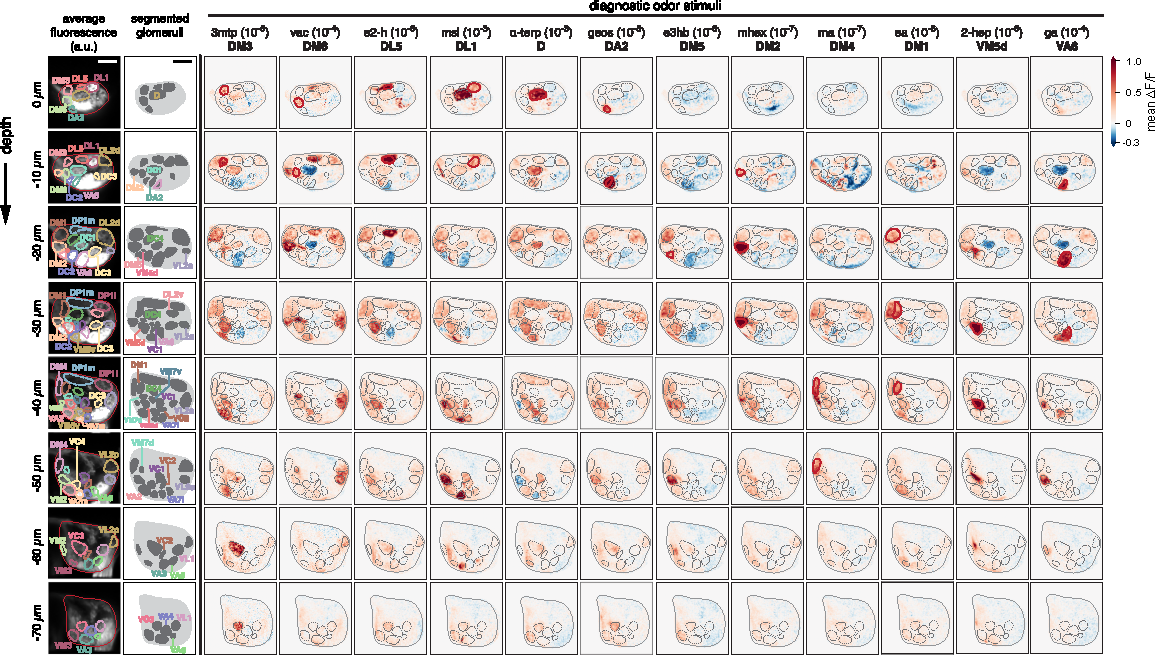
\includegraphics[width=0.875\textheight, angle=-90, origin=c]{s1_full_diagnostic_guide_page1}
% TODO what's the logic behind the "segmented glomeruli" betty decided to show? doesn't even include all the ones targeted directly by diagnostics (e.g. DL5), nor other ones labelled like DP1m (between it and the stuff to the left, should show all segmented. bit confusing)
\mycaptionof{figure}{Example diagnostic odor volumetric ORN responses}{%
All identified glomeruli are shown across left two columns.
Example responses of one fly to first 12 of 24 ``diagnostic'' odors.
(continued on next page)
}
\label{fig:s1}
\end{longcapfigure}
\begin{figure}[H]
\ContinuedFloat
\centering
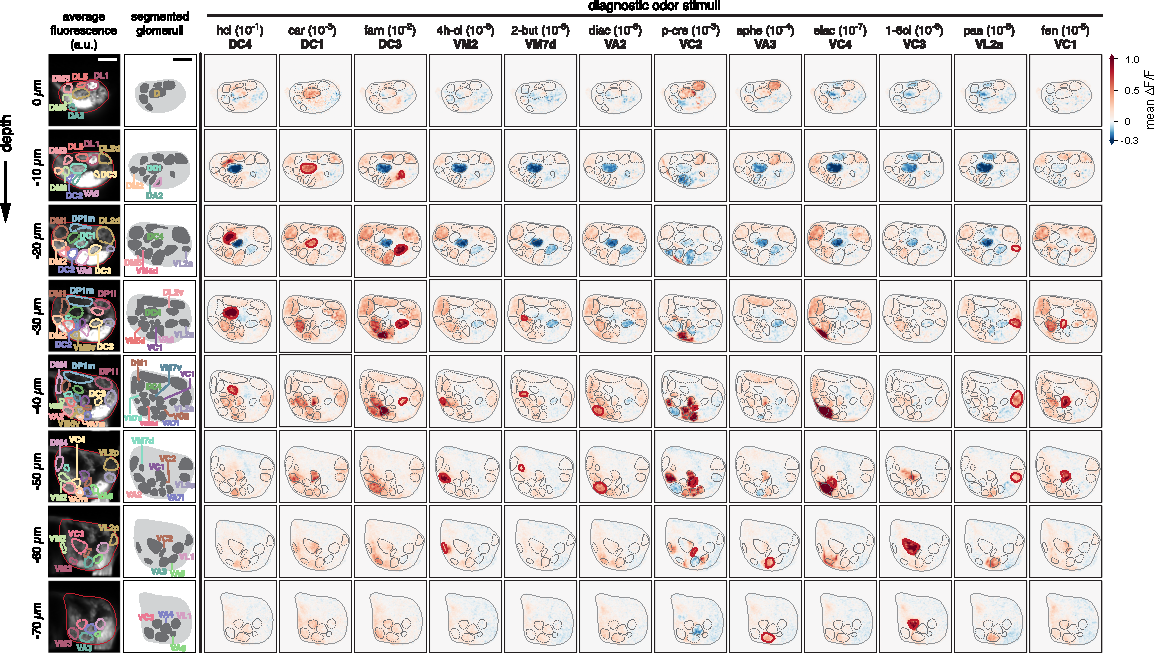
\includegraphics[width=0.875\textheight, angle=-90, origin=c]{s1_full_diagnostic_guide_page2}
\caption[]{\textbf{Example diagnostic odor volumetric ORN responses (continued).}
Left two columns same as on previous page.
Example responses of one fly to remaining 12 of 24 ``diagnostic'' odors.
}
\end{figure}
% }

% Figure S2 - Diagnostic example mean response and all individual fly responses
% {
\begin{longcapfigure}
\centering
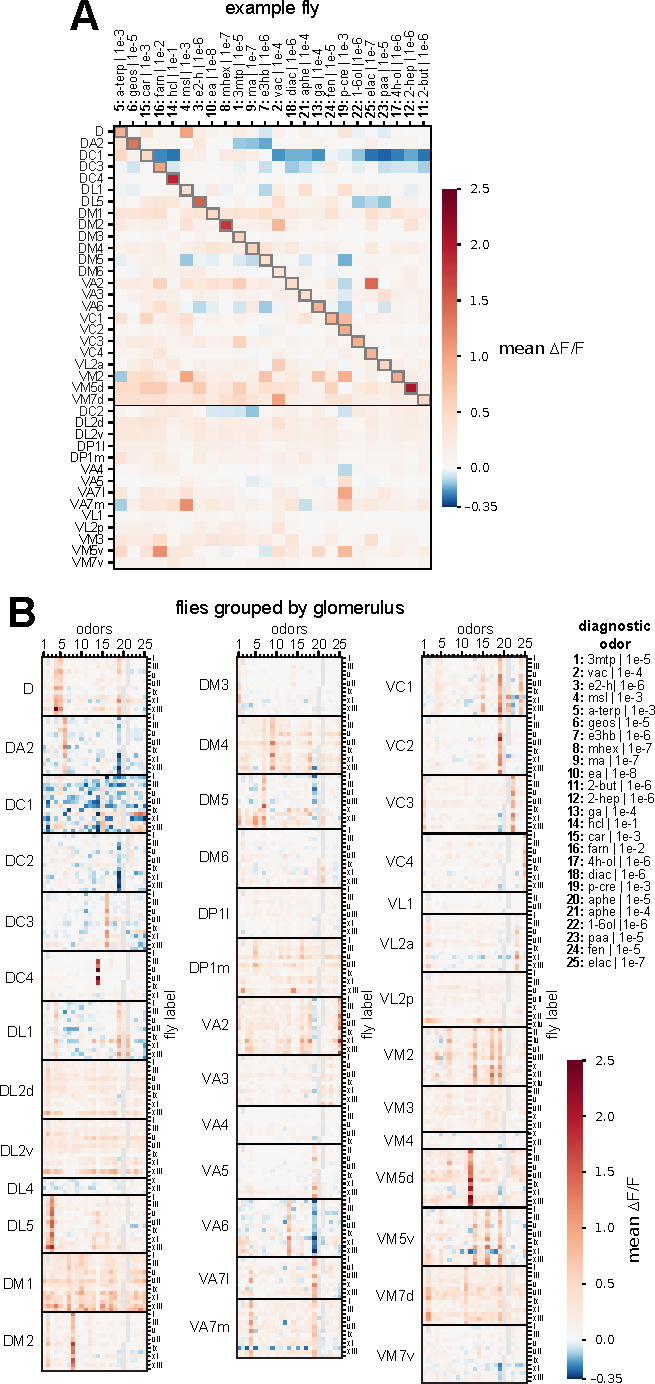
\includegraphics[height=0.875\textheight]{s2_diagnostic_example}
\mycaptionof{figure}{Example per-glomerulus diagnostic odor responses and variation across flies}{}
\label{fig:s2}

% TODO was this the same fly as in previous figure? say so, if so
\mysubcaption{A}{%
Trial-mean responses to the diagnostic panel in one example fly.
The first 24 rows are the odors presented in this fly, sorted by which glomerulus they are intended to target, with the responses in these target glomeruli boxed along the diagonal.
The remaining rows are glomeruli that were identified based on the context provided by the responses to the diagnostic odors, combined with the expected shape and position of the glomeruli\cite{ALAtlas}.
}

% TODO TODO change language to clarify that filtering was WITHIN panel (>= half)
\mysubcaption{B}{%
Trial-mean responses to the diagnostic panel for all 40 glomeruli identified in $\geq\!\text{half}$ of ORN terminal flies (across the two odor panels).
Excitatory responses in particular are typically quite stereotyped across flies.
However, some glomeruli (e.g. DM1 and DP1m) respond weakly and to many odors, with the overall activation strength partially dependent on the particular fly.
After the first seven flies (all from the first odor panel), we changed the concentration of aphe from $10^{-5}$ to $10^{-4}$, to elicit stronger responses in the VA3 glomerulus this odor targets.
The first two flies are missing data for vac.
}
\end{longcapfigure}
% }

% Figure S3 - ORN/PN means/SDs/per-glomerulus sample sizes
% {
\begin{longcapfigure}
\centering
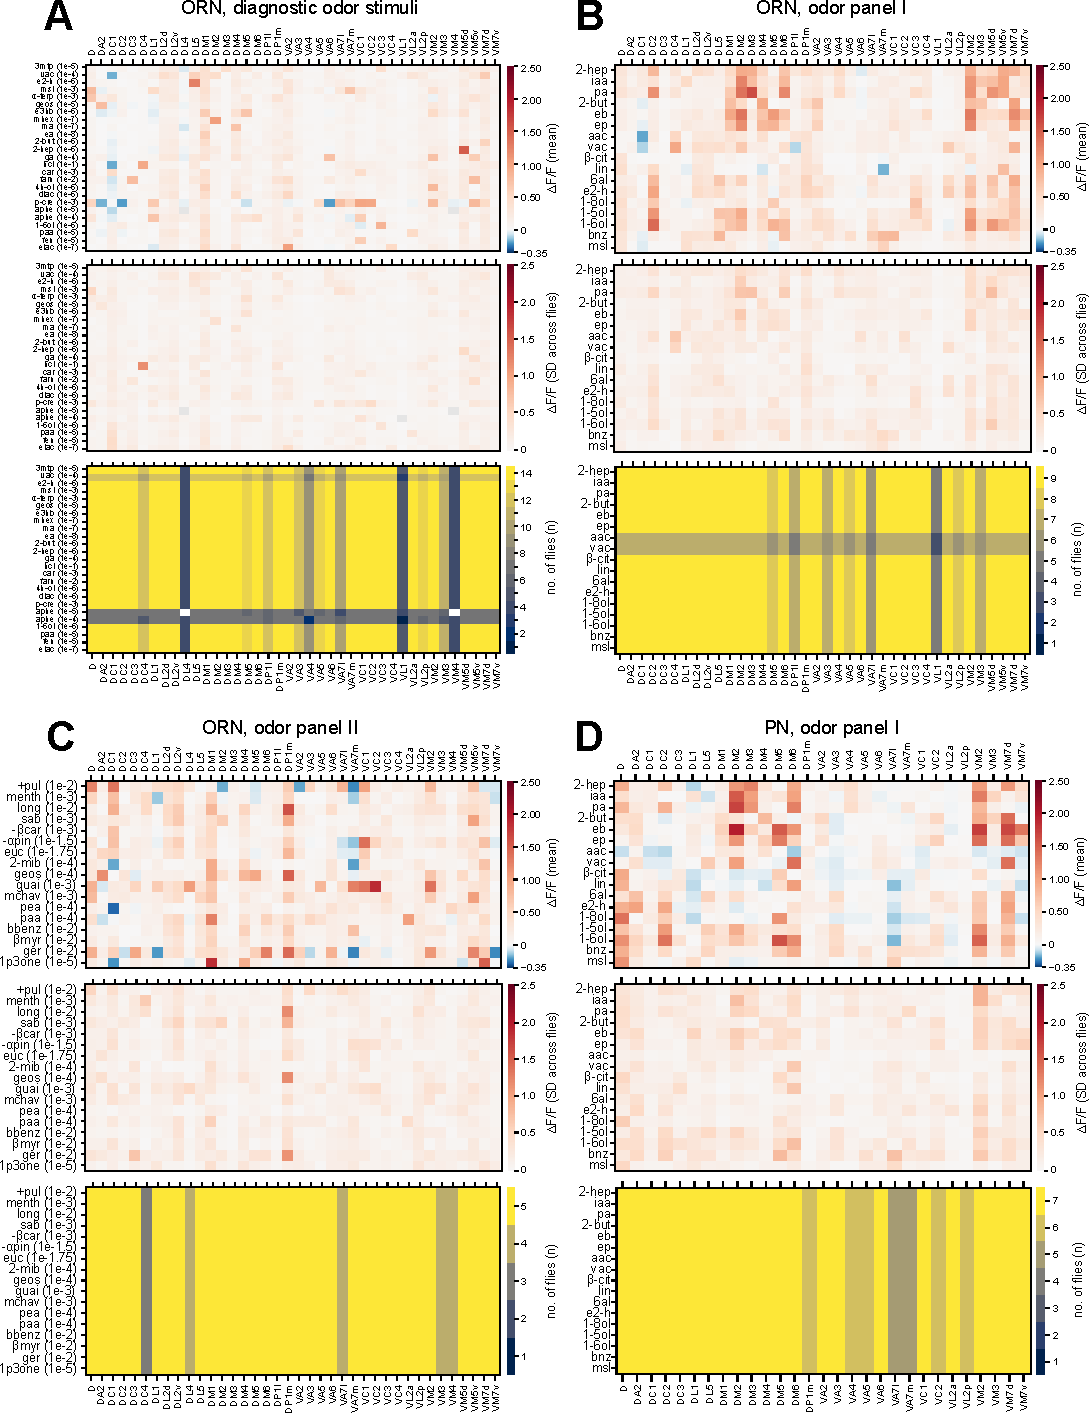
\includegraphics[width=\textwidth]{s3_orn-pn-mean-err-n_fixed}
\mycaptionof{figure}{Per-glomerulus response means, SDs, and sample sizes}{%
All panels contain the per-glomerulus response means (top), SDs (middle) and sample size (\# flies) (bottom).
All mean response plots share the same colorbar limits, and share the non-negative portion of the colorbar with the SD plots.
}
\label{fig:s3}

\mysubcaption{A}{%
ORN terminal responses to the diagnostic panel, from flies across both of the experimental panels.
}

\mysubcaption{B}{%
ORN terminal responses to odor panel one.
}

\mysubcaption{C}{%
ORN terminal responses to odor panel two.
}

\mysubcaption{D}{%
PN dendrite responses to odor panel one.
% TODO 70% of glomeruli or of PNs? matter? (say PNs elsewhere, in original text that said 70%)
The GH146-Gal4 driver we used for PN imaging only expresses in \textasciitilde70\% of glomeruli\cite{GH146}, hence the smaller number of glomeruli identified.
}
\end{longcapfigure}
% }

\begin{longcapfigure}
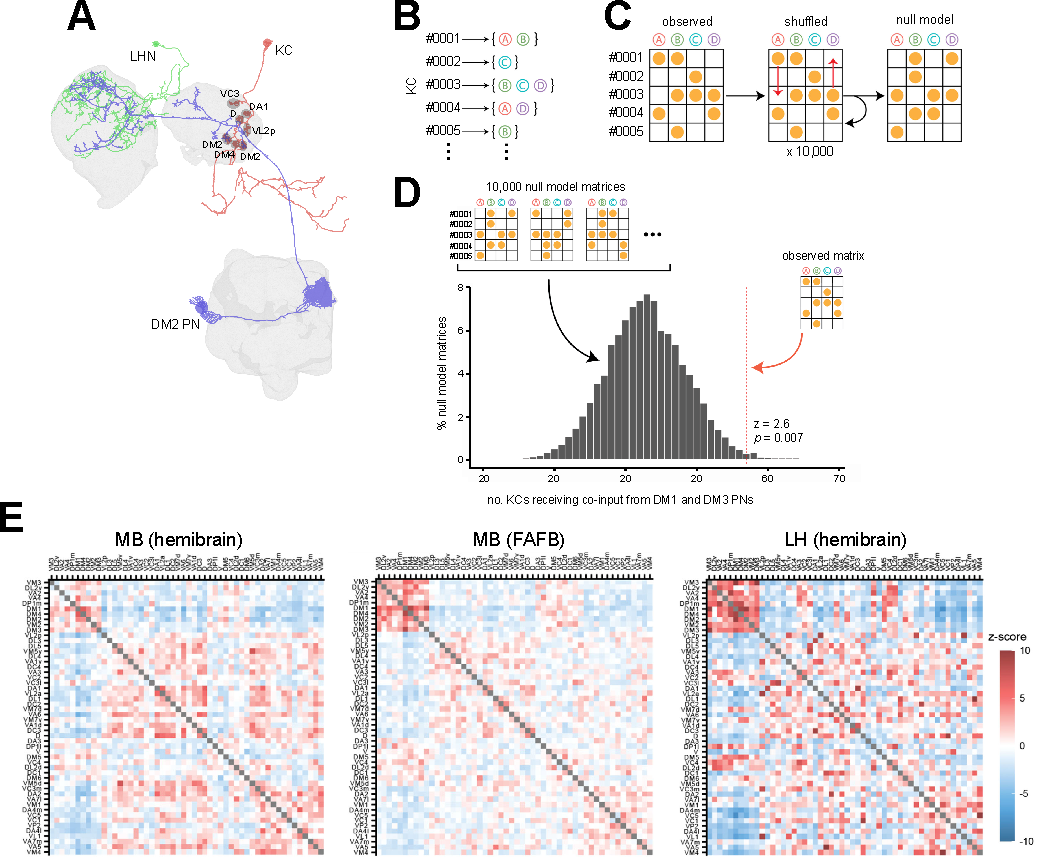
\includegraphics[width=\textwidth]{s4_hemibrain_fafb_hb-lh_overconvergence_NO-HEMIDRAW}
%
% TODO delete (if wanting to keep hemidraw and cosine distance supplemental panels F-H)
% (most moved to start of new S5, except H basically)
%\includegraphics[width=\textwidth]{s4_hemibrain_fafb_hb-lh_overconvergence_WITH-HEMIDRAW}
% (adapted from preprint caption)
%
\mycaptionof{figure}{The structure of olfactory glomerular inputs to third-order olfactory neurons}{}
\label{fig:s4}

% TODO need to adapt any of these preprint captions?
% TODO TODO why do we redefine KC and LHN here but not PN? be consistent
\mysubcaption{A}{%
Example reconstruction from the hemibrain connectome\cite{Hemibrain} of a uniglomerular DM2 PN and two example postsynaptic partners, a Kenyon cell (KC) and a lateral horn neuron (LHN).
Synaptic connections between identified neurons contained within the hemibrain volume are fully described.
}

% TODO need to adapt any of these preprint captions?
% TODO can i really not just condense B/C/D into one letter? care?
% Prat recommended these FAFB citations, and in this order
\mysubcaption{B}{%
For each third-order olfactory neuron, the set of glomeruli providing direct presynaptic input via PNs was extracted from connectome datasets (hemibrain and FAFB)\cite{Hemibrain,FAFB0,FAFB1,FAFB2}.
For this analysis, synaptic connections were binarized (e.g., all glomerular inputs >5 synapses were treated equally regardless of synapse count).
}

\mysubcaption{C}{%
The mapping of glomerular inputs to KCs was represented as a binary matrix, where a 1 in $\text{cell}_{i,j}$ indicates that neuron $i$ receives input from glomerulus $j$.
The `Curveball' algorithm was used to generate random matrices (null model) that preserve the row and column totals of the original matrix\cite{CurveballMatrixRandomization}.
}

\mysubcaption{D}{%
For each pair of glomeruli, a distribution of the number of KCs receiving co-input from the two glomeruli in each shuffled matrix was generated.
The observed number of KCs receiving co-input from each pair of glomeruli in the hemibrain was compared to this distribution to generate a $z$-score.
An example distribution and $z$-score for the over-convergent glomerular pair DM1 and DM3 are given.
}

% Prat recommended these FAFB citations, and in this order
\mysubcaption{E}{%
Glomerular input structure to KCs in the hemibrain MB\cite{Hemibrain} (left), KCs in the FAFB MB\cite{FAFB0,FAFB1,FAFB2} (center), and LHNs in the hemibrain LH (right).
The $z$-score for each pair of glomeruli measures the degree to which the glomeruli are over- or under-convergent in the observed population, compared to null models.
A large positive value indicates strong over-convergence, and a large negative value indicates strong under-convergence.
The ordering of glomeruli is the same in all matrices and was based on $k$-means clustering of the hemibrain MB matrix. 
}
\end{longcapfigure}

% Figure S5 - Model APL/threshold sensitivity analysis, KC vs model response rates[, hemidraw]
% {
\begin{longcapfigure}
% TODO break B,C into a separate figure (so caption isn't so awkward, at least), with them arrange in one column?
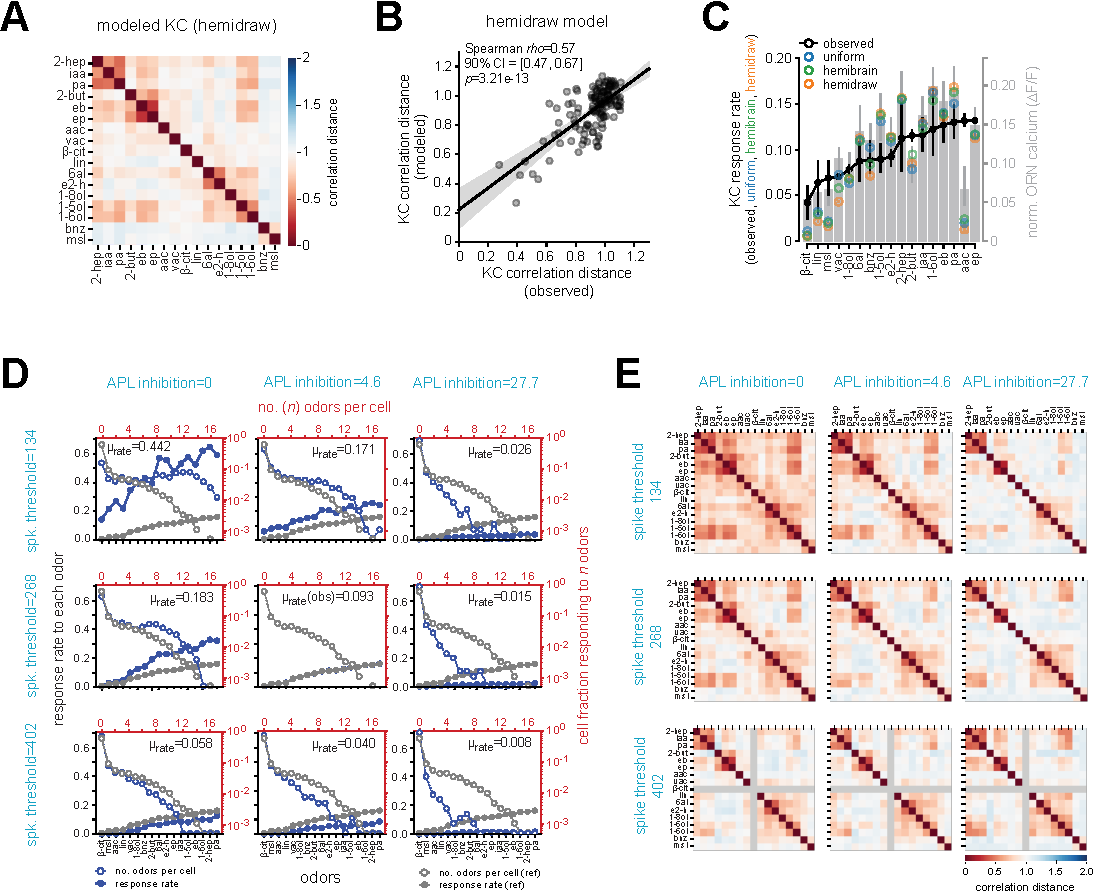
\includegraphics[width=\textwidth]{s5_apl-thr-sens_and_model-vs-kc-responsivity_WITH-HEMIDRAW}
% TODO better caption?
\mycaptionof{figure}{Model (vs observed) KC response rates and sensitivity analysis}{}
\label{fig:s5}

% TODO TODO TODO actualy refer to A,B,D,E in text (maybe just methods?)
% currently only talk about C
\mysubcaption{A}{%
Matrix of pairwise correlation distances ($1 - \text{Pearson's } r$) between predicted KC responses in the `hemidraw' model for the 17 odors in odor panel one.
Each KC in this model variant independently draws 7 glomerular inputs (as the `uniform' model), but with the probability of drawing each glomerulus determined by the PN-KC synapse counts in the hemibrain connectome (see Methods).
}

\mysubcaption{B}{%
Comparison of observed and `hemidraw' model KC odor-odor correlation distances, for odor panel one (as \cref{fig:3:E} does for `uniform' and `hemibrain' models).
Each point represents one odor pair ($n{=}136$); observed KC distances are averaged across flies ($n{=}4{-}18$); hemidraw model KC distances are averaged across 100 instantiations of the model.
The line shows the linear fit between modeled and observed distances, with 95\% CI of the fit shaded (from a bootstrap over odor pairs).
% TODO TODO is this CI (on the rho) actually from bootstrapping across odors pairs? check code
The Spearman's $\rho$ between the hemidraw model and observed KC distances is $0.57$ (90\% CI 0.47--0.67; $p{=}\num{3.2e-13}$).
}

% TODO delete? and in fig:3 above too?
%CIs were computed from a bootstrap over odor pairs.

% TODO refer to thresholding details? say model cells were considered as responding if they spiked at least once?
% TODO how to format roman numeral?
\mysubcaption{C}{%
Response rates to odor panel one in KCs and in uniform, hemibrain, and hemidraw model KCs.
}

% TODO TODO rename "APL inhibition" (-> "scale of KC<->APL weights") in plot (since it's also the KC->APL drive)
\mysubcaption{D}{%
Sensitivity analysis sweeping KC spike threshold (a constant relative to spontaneous input each KC receives) and scale of \APLKC weights.
Model with ``tuned'' values for KC threshold and APL weight scales are in the center of the grid, with threshold stepped across rows and APL weight scale stepped across columns.
APL weight is not stepped to the same extent in the decreasing direction, because the \APLKC weights can not be negative, but APL inhibition is completely disabled in this 0-weight case.
% TODO roman numeral formatting for odor panel I?
Each panel plots the distribution of the \# of odors each KC responds to (top \& right axes, with red labels; plotted as open points), and the mean response rate (across model KCs) to each odor (bottom \& left axes, with black labels; plotted as filled points).
% TODO check claude
%Odors (lower X-axis labels) for each response rate plot are ordered by the tuned response rates (note that this differs from the order in (A), where odors are ordered by observed KC response rates).
Odors (lower X-axis labels) for each response rate plot are ordered by the tuned response rates (note that this differs from the order in \textbf{(C)}, where odors are ordered by observed KC response rates).
Each panel has the tuned values re-plotted (from the center panel) in gray for reference.
% TODO TODO move some of this to method or something?
% TODO reword? delete
The higher step for the threshold and APL weight scale can each, individually, bring the KC response rates down dramatically.
Only a single digit number of KCs responds to each odor in both increased APL weight scale cases, and in the bottom right (where the threshold is also increased) one odor (\BCit) evokes no KC responses.
}

% TODO TODO retry w/ computation including non-responders (and then also add some noise?) (and compare against KC calculation that also includes non-responders)
\mysubcaption{E}{%
Odor-odor correlations (within KCs responding to at least one odor) at the same steps as in \textbf{(D)}.
Observed decorrelation is not achieved even with extreme values for these two parameters, where very few KCs are responding.
% TODO mention relationship between the two weights here, or just in methods?
}
\end{longcapfigure}

\begin{longcapfigure}
\centering
% even with only one line for caption label (and the following "(captions on next page)" line), 0.9 is too much
% (causes blank page before)
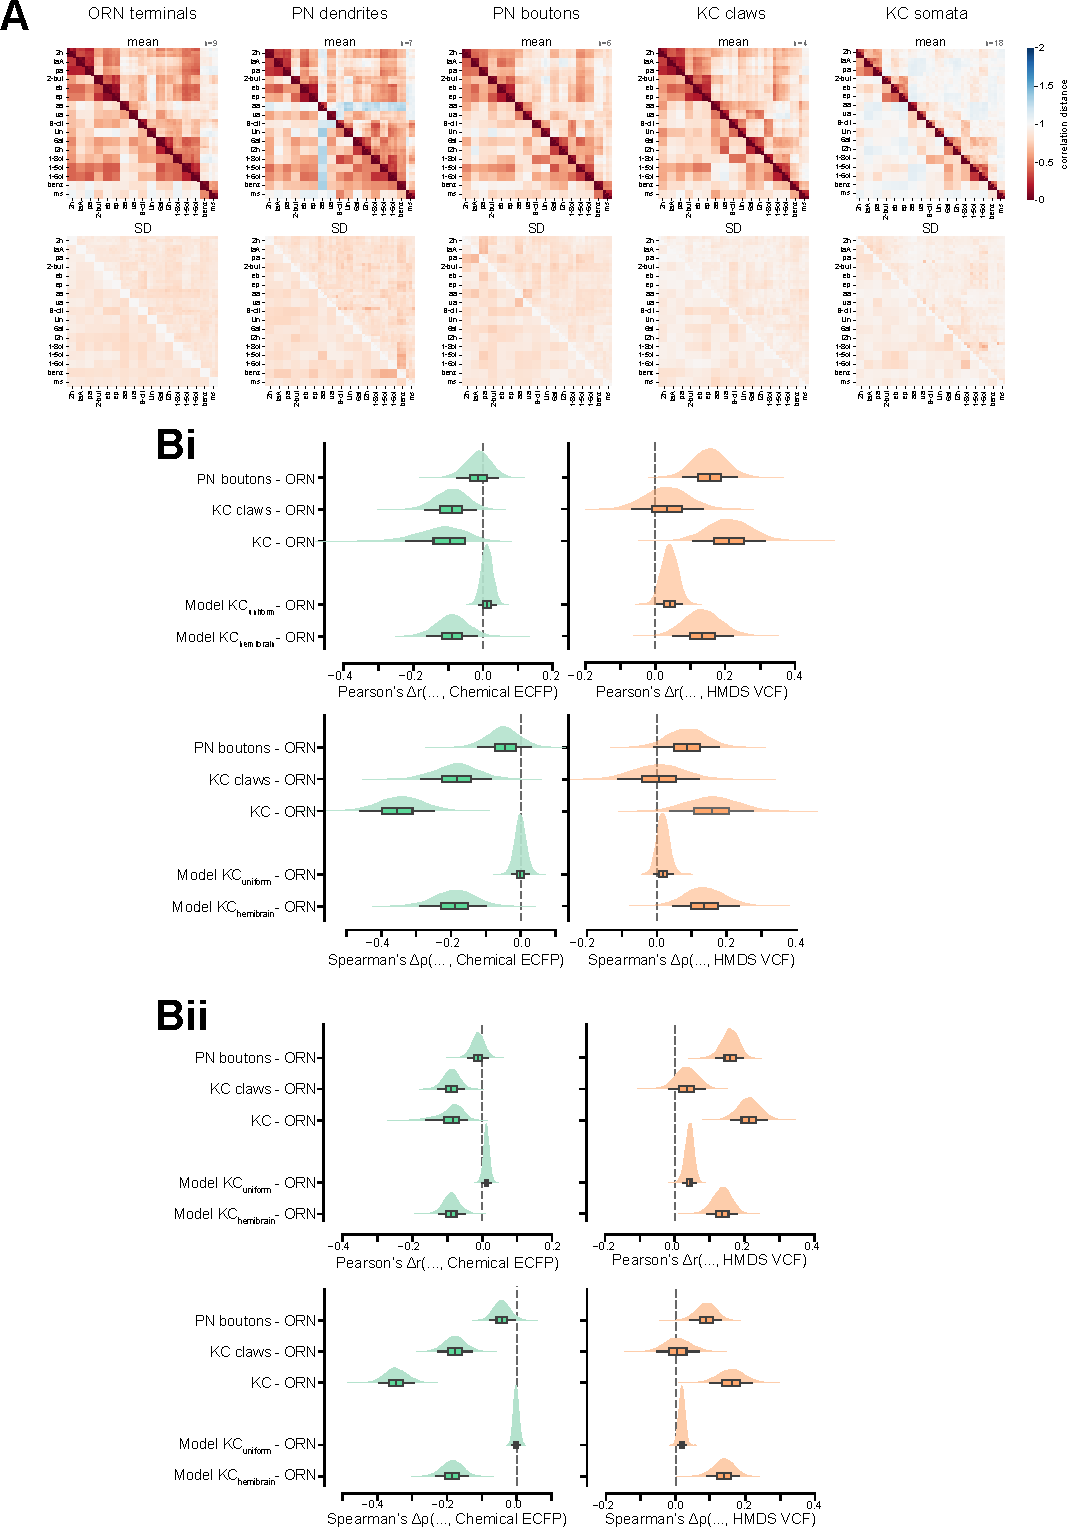
\includegraphics[height=0.875\textheight]{s6_corr-errs-and-space-minus-orn-comps-replacement-v-not}
% TODO is this the only place where SD for megamat corrs are shown? (think so) (and do we even show them for validation2 anywhere then?)
% delete A if shown elsewhere?
% TODO better caption?
\mycaptionof{figure}{Neural RDM SDs and changes of neural alignment with chemical/natural-source spaces relative to ORNs}{}
\label{fig:s6}

\mysubcaption{A}{%
Odor-odor correlation distances ($1 - \text{Pearson's } r$) between odor representations in ORN terminals ($n{=}9$), PN dendrites ($n{=}7$), PN boutons ($n{=}6$), KC claws ($n{=}4$), and KC somata ($n{=}4{-}18$).
Top row, mean Pearson correlations across flies.
Upper triangle: trial-trial correlations.
Lower triangle, correlation between trial-averaged odor representations.
Bottom row, standard deviation of Pearson correlations across flies, with upper and lower triangles arranged as in the top row.
}

\mysubcaption{B}{%
Change in each stage's correspondence with chemical structure (left, green) and natural source (right, orange), relative to ORN terminals: $\Delta = corr(\text{stage}, \text{reference}) - corr(\text{ORN terminals}, \text{reference})$.
Each correlation is computed across the 136 odor pairs between each stage's mean odor-odor dissimilarity (\Cref{fig:6:C}) and the reference space distances.
Rows: PN boutons, KC claws, KC somata, and modeled KCs (uniform and hemibrain).
The reference spaces are grouped by column: left (green) plots show correspondence with chemical structure space (computed from ECFP fingerprint distances); right (orange) plots show correspondence with natural-source space, with distances computed from a 3-D hyperbolic embedding of compounds based on their occurrence in the Volatile Compounds in Food database.
Both Pearson's $\Delta r$ (upper row) and Spearman's $\Delta \rho$ (lower row) are shown; dashed line indicates no change from ORN terminals.
Boxes indicate the mean and interquartile range; whiskers show central 90\% of each resampling distribution.
}

\mysubcaption{Bi}{%
Bootstrap, with \num{5000} draws of the 136 odor pairs with replacement, using the same odor pairs for each stage and the ORN terminals when computing.
}

\mysubcaption{Bii}{%
Subsampling, with \num{5000} draws of 80\% of odor pairs without replacement.
}
\end{longcapfigure}

% NOTE: this may be a table in text, but i think i want it as a figure for thesis at least
% Also, remy may have her own supplement fig 7 regarding main text fig 7, but since I'm including
% neither of those, I'm numbering this one S7.
\begin{longcapfigure}
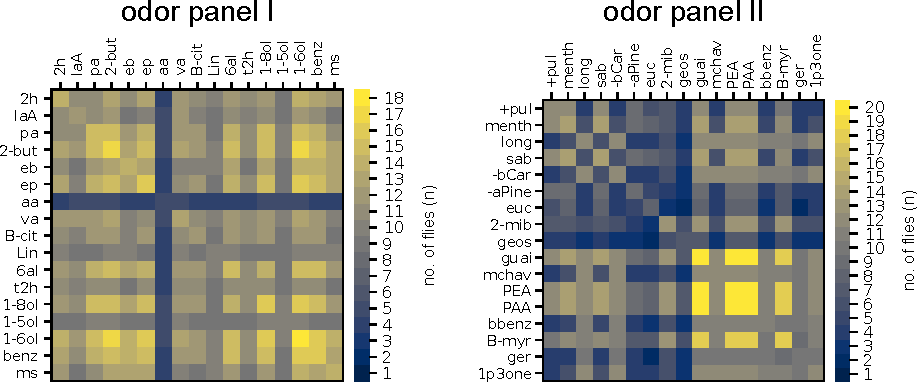
\includegraphics[width=\textwidth]{my_s7_odor-pair-n}
\mycaptionof{figure}{KC soma sample sizes for odor pairs within brains}{%
As not all odors are presented in each fly, for these KC soma datasets, we report the sample size $n$ (\# of flies) for which both odors are measured together in the same fly.
Odor panel I (left) has a minimum of $n{=}4$ flies, while panel II (right) has a minimum of $n{=}2$ flies.
}
\label{fig:s7}
\end{longcapfigure}

% TODO move into supplementsection def? (can't seem to, at least not in the place i tried)
\processdelayedfloats
% }

% NOTE: i think this must contain its own refsection, cause it complained when it was before t he end of the refsection above
% TODO TODO this work? (want after the floats?)
% TODO TODO actually want this? why? it looks like another mini-bibliography, but i think it's confusing
%
% TODO TODO or move to start? saw at least one in tarun's that i think did it more like that
%\publishedas{RemyPreprint}

%

\chapter{Searching for principles explaining third-order olfactory neuron responses to simple and complex mixtures}
\label{chap:natmix}
\begin{refsection}

\section{Introduction}
Understanding the encoding of mixtures is fundamental to olfaction, as most natural odors are composed of many component chemicals, frequently dozens\cite{VCF}.
In \cref{sec:sampling_difficulty}, I discuss the challenges of identifying and quantifying the concentrations of component volatiles in natural odors, and the additional challenge of determining which are perceptually relevant.
Beyond knowing what is in a natural mixture, or basic properties like which chemicals frequently occur together or typical distributions of component concentrations, we are also faced with the challenge of actually constructing and delivering an odor mixture to the animal.

Unlike vision, where our knowledge of optics and the tuning of the three types of human photoreceptors allows us to build displays which can generate arbitrary images, generating synthetic mixture stimuli unfortunately requires sourcing and physically mixing the desired component chemicals.
Mixing in gas phase requires complicated olfactometers to ensure each component gets the target flow, which often limits the number of components.
On the other hand, mixing in liquid phase limits the mixtures that can be selected during an experiment, and can be a major experimental burden.
Both approaches ultimately can suffer from odor contamination inside the olfactometer, and many receptors can detect odors down to very low concentrations, further complicating stimulus delivery and interpretation of data\cite{TraceFIDOlfResponses}.

One set of approaches uses the same chromatography, as is used to separate chemicals for identification/quantification, to separate components for independent olfactory presentations\cite{BananaCode}.
These approaches are elegant in that they can use natural sources as input, rather than needing to separately source each component chemical, however the process of collecting/sampling volatile mixtures for chromatography can impose distortions on the ratios of sample chemicals\cite{ConcentrationReview}.
It is also difficult to use these approaches to present subsets of the components of a natural mixture, and although some work has developed solutions to this problem, it introduces further complexity while suffering from the same distortions on the individual components\cite{GCRecombination1,GCRecombination2,GCRecombination3}. 

The only real alternative may be to optogenetically activate certain patterns of receptor neurons, and although this has been done, it has major downsides that prevent it from being a general solution\cite{Jeanne2018,Chong2020}.
Optogenetic activation can not always achieve the firing rates that can be evoked by odors, especially the high firing rates seen in \textit{Drosophila} ORNs (which can often reach \textasciitilde\qty{300}{\hertz}), while also imposing enormous additional experimental difficulty\cite{Fişek2021}.
The genetics to introduce these photosensitive channels also limit what other genetic (or optogenetic) manipulations can be made.

One might naively assume that mixtures should evoke stronger responses than any of the components, as all the components are still present (at the same concentration, typically), and there is more total odor delivered to the animal. 
However, at least when looking at individual cells or glomeruli, there is a wide body of work describing what is frequently called ``mixture suppression'', where a mixture elicits a response smaller than the responses to the strongest component\footnotemark[1]{}.
\footnotetext[1]{Many studies compare mix responses to the sum of component responses instead, but it often does not matter. See \cref{ssec:mix_supp_def}.}
This has been observed across multiple levels of the olfactory system, from interactions between odors (or their responses at): the receptors themselves\cite{ORNLinearMixWithInh,CompetitiveBinding,ReceptorInh2,ReceptorInh3,DiverseORInteractions,Zak2020}, ORNs (called OSNs in mammalian literature) \cite{DuchampViret2003,EphapticSensillaInh,Xu2020,Wu2022}, PNs or similar mammalian mitral/tufted (M/T) cells\cite{Davison2007,Silbering2007,Mohamed2019}, and KCs or similar mammalian piriform cortex (PCx) neurons\cite{PiriformMixSupp,Rokni2020}.
At the receptors themselves, mixture suppression can be explained in terms of either competitive binding, antagonism, or inverse agonism\cite{MurthyAntagonism,CompetitiveBinding,Inagaki2020}, and is increasingly seen as a widespread effect.
Some mixture suppression between \textit{Drosophila} ORNs has been described as the result of ephaptic coupling between ORNs housed in the same sensilla\cite{EphapticSensillaInh,Wu2022}, but measurements at the output terminals in the AL or olfactory bulb (OB) may also include effects of GABAergic lateral inhibition.
PN or M/T cells can exhibit mixture suppression from additional stages of AL/OB GABAergic lateral inhibition\cite{Olsen2010}, as well as inheriting any in prior stages.
KCs or PCx neurons have their own feedback inhibition which can contribute to new varieties of mixture suppression, and can once again inherit this type of tuning from their inputs.

Although they may be less frequent, and often more circumstance specific, there are also examples of the opposite behavior (``synergy''), where responses to the mix are above the max (or sometimes the sum) of component responses.
These effects also range from the level of the receptors\cite{Kundu2016,DiverseORInteractions,HumanPositiveAllostery}, the ORNs/OSNs\cite{MosquitoORNHumanOdorSynergy,Xu2020}, to the PNs\cite{Das2017,Zocchi2022}, and again have a diversity of mechanisms.
Between these two extremes, many studies also report many mixture responses that lie somewhere between the representations of the individual components\cite{PiriformMixSupp,Campbell2013,Endo2020}.
% examples of synergy:
% Kundu2016 (ORN receptor, not ephaptic)
% HumanPositiveAllostery (receptor)
% subset of data from DiverseORInteractions
% MosquitoORNHumanSynergy (ORNs)
% another set of data from Xu2020 (OSNs)
% PNSynergyeLNGapJunction (Das2017) (PNs)

Interactions between the percepts of the components can also be complex, and it can be difficult to predict the percept of the mixture as a result.
Many mixtures are perceived as distinct objects (``configurally''), with a percept completely different from those of the components, even for simple binary mixtures\cite{Jinks1999,Jinks2001}.
A classic example of this phenomenon is how the mixture of ethyl isobutyrate (perceived to humans as strawberry) and ethyl maltol (caramel) is perceived as pineapple, a specific trick that also seems to work on other species including honeybee, rabbits, and mice\cite{Wycke2020}.

Synergy as described above could contribute to configural representations, but it may not be necessary to invoke any of these effects to explain mix-selective (i.e. configural) responses that may arise in KCs.
Since KCs quasi-randomly sample multiple PNs (and typically require multiple co-active inputs to spike) it seems reasonable to expect some KCs to be mix-selective, assuming there are KCs that sample PNs that separately respond to the components.
Surprisingly, when \textcite{LocustKCMixSpiking} recorded from locust KCs, they report that the majority of their KCs ``segment'' individual components, where if they respond to a component, they also tend to respond to most mixtures that contain that component.
Although they mention seeing some number of mix-selective KCs, they do not break down how many cells they see with each type of tuning, and there are concerns that their experimental approach biased them towards finding the ``segmenting'' cells they see so frequently\cite{LocustKCMixSpiking}.
Like other studies that have recorded KC or PCx responses to complex mixtures, they are only able to sample a small fraction of the total KC population\cite{PiriformMixSupp}.
Several other studies do show signs of mix-selective populations of third-order neurons (KCs or PCx neurons), but typically smaller than other populations and often with experiments only using binary mixtures or with other major limitations\cite{PiriformMixSupp,Rokni2020,Endo2020}.
Do we see mix-selective KCs, when sampling the entire population?
If so, what fractions of the KCs exhibit this behavior (compared to the populations with other types of tuning), and how do these populations vary with the complexity of the mixtures?

In this study, we characterize odor mixture encoding across the full populations of both ORNs and the third-order KCs.
This represents the first time such complete input and higher-order olfactory representations have been measured to precisely controlled mixtures of >2 components.
Prior work has either been limited to sampling only a small subset of the neurons\cite{LocustKCMixSpiking}, only focused on binary mixtures\cite{Endo2020}, or both\cite{PiriformMixSupp,Campbell2013}.

We find that the majority of responding KCs respond selectively to single components, with the response to the mix dramatically suppressed (relative to the maximum component response).
This mixture suppression is particularly strong in our experiments with five-component mixtures, in contrast to the binary mixtures typically studied in prior work.
Despite other studies seeing strong antagonism in the receptor responses to many odors, our ORN measurements are inconsistent with much of this KC suppression being inherited from the ORN responses.
We also use our ORN measurements to construct model KC responses, expanding on a previously described biophysically-plausible model of the fly MB\cite{Kennedy2019}, and we are able to recapitulate some KC response features, including some of the mixture suppression observed in our complex mixtures.
However, the degree of observed KC mixture suppression exceeds our model predictions to all mixtures, implying a mismatch between the model assumptions and the biology.
This mismatch suggests that there are circuit mechanisms or neurons whose role in complex mixture processing are not yet appreciated.

\section{Results}
\subsection{Mixture design}
As we hope to describe general mechanisms by which natural odors are processed, our first goal was to construct mixtures that had concentration and intensity distributions (across the monomolecular components) that more closely resembled those distributions in natural mixtures.
In choosing the mixtures to study, we wanted enough components to move in the direction of the stimulus complexity of natural mixtures (which often have >10 perceptually relevant components), but also few enough to keep downstream experiments tractable\cite{BananaCode,GCRecombination3}.
For this tradeoff, we chose to design mixtures of five monomolecular components.

% TODO delete or de-dedupe w/ last paragraph below at least (i do like that this doesn't explicitly say most activating 2, at least...
%For each of the two 5-component mixtures we describe below, we also included 2-component (``binary'') variants in our experiments, by subsetting each full 5-component mixture to the two components driving the most ORN activity\footnotemark[1]{}.
%These simpler mixtures could help identify properties of mixture encoding that may be generally related to the number of mixture components.
% TODO just move to KC section?
%For the simpler 2-component mixtures, we also did a series of KC experiments where we presented each mixture and their components at 10 and 100-fold further dilutions (volume/volume), as well as the original concentrations.
%These experiments could identify properties of mixture encoding that vary with concentration (or response intensity) scale, and are more tractable when restricted to the binary mixtures.

% Kiwi chromatogram
\begin{longcapfigure}
\centering
% TODO set fixed size?
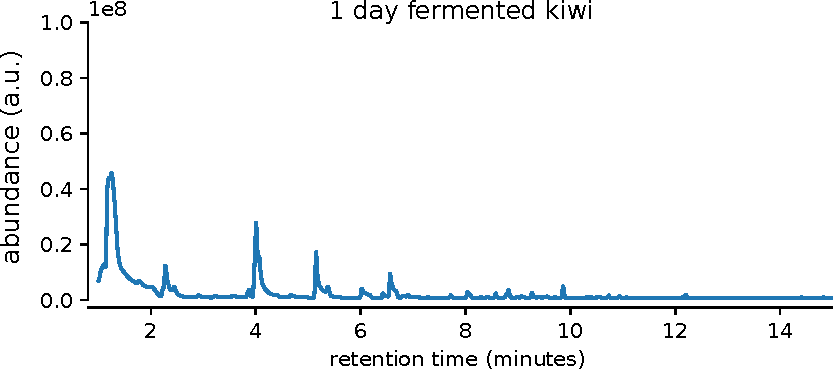
\includegraphics[width=0.6\textwidth]{kiwi_chromatograms_day1-fermented-only}
\mycaptionof{figure}{Chromatogram of lightly fermented kiwi headspace}{%
% TODO list major peaks by retention time (what are they tho...)?
Chromatogram of fermented kiwi headspace volatiles, including the five major components we selected for mix A (\cref{table:mix_odors}).
}
\label{fig:kiwi_chromatogram}
\end{longcapfigure}

% TODO move some of this to methods? prob not most of it
The first mixture I constructed (``mix A'') was based on chemistry I did to describe the headspace components of an odor likely to be appetitive to flies: kiwi in the early stages of yeast fermentation.
I used gas chromatography-mass spectrometry (GC-MS) to characterize the headspace of a fermenting kiwi sample, and identified the five most abundant compounds (see Methods; \crefwithbackref{fig:kiwi_chromatogram}).
Although using more components would likely result in a better approximation of the fermenting kiwi percept, I limited the mixture to the top five components (again, to limit experimental complexity).
It is not necessarily the case that the components with the highest GC-MS peak area are those with the highest concentration (because different chemicals have different response factors with the MS detector), and it is also possible that lower concentration components could be more perceptually important, but this seemed a reasonable place to start.
The components of mix A are ethyl butyrate, ethyl acetate, isoamyl acetate, isoamyl alcohol, and ethanol.
Several of these odors are among the more abundant components of many different fruits, and several also individually have a fruity percept to humans\cite{VCF,GoodScents}.
The concentrations and plot abbreviations we chose for these odors are in \crefwithbackref{table:mix_odors}.

%Our chemistry gave us one loosely naturalistic odor mixture, but we also wanted to include at least one additional mixture to study.
We also wanted to study a mixture of similar complexity, but with compounds unlikely to appear together in natural sources.
We constructed a second mixture (``mix B''), composed of five compounds (to match the number of components in mix A), aiming to include a greater diversity of component percepts and chemical classes than in mix A.
After choosing these five components, we still needed to choose their concentrations.
We selected concentrations that would, across the set of components, produce a similar distribution of ORN activation strength to the components in mix A.
The components of mix B are 1-octen-3-ol, 2-heptanone, furfural, valeric acid, and methyl salicylate.
The concentrations and abbreviations we chose for these odors are also in \cref{table:mix_odors}.

To determine the extent to which responses to our mixtures are dominated by the interactions of a small number of strongly activating components, we constructed binary mixtures from the two most activating components of each of our five-component mixtures.
The components of binary mix A are ethyl butyrate and ethyl acetate, and the components of binary mix B are 1-octen-3-ol and 2-heptanone.
These mixtures also helped us start to investigate the more general role of the number of components in mixture encoding.

% TODO delete?
%\footnotetext[1]{Preliminary experiments to determine stimulus intensity used electroantennography (EAG), and although preliminary imaging data seemed mostly consistent with the EAG data (data not shown), 2-heptanone no longer seems to be among the two most activating components in the current ORN imaging data}

\subsection{Mixtures activate KCs less on average than individual components}
We started our investigation of mixture encoding in the KCs.
To what extent would we see mixture representations intermediate to component representations, as in \textcite{Campbell2013} or \textcite{Endo2020}?
% claude complains about as <what>, but i'll leave it
Would we see cells that respond to components regardless of whether they are alone or in various mixture contexts, as \textcite{LocustKCMixSpiking}?
Would we see cells that respond selectively to our mixtures, as the random sampling of PNs by KCs might suggest?
Was the mixture suppression that is seen in multiple levels of olfactory processing\cite{PiriformMixSupp,Zak2020} also a prominent feature in our KC responses?

We presented our mixtures and components while recording the responses of whole KC populations.
KC responses to odors were defined as the \KCRespStat, where $F_c$ is the neuropil-subtracted fluorescence activity trace for each ROI (extracted via Suite2p)\cite{Suite2p}.
After \textit{Z}-scoring the entire activity trace, responses were calculated by subtracting a pre-stimulus baseline from each odor response (see Methods).
We clustered the responses in \Crefwithbackref{fig:clust_hierarch_binary} and \refwithbackref{fig:clust_hierarch_5comp}.

% Mix A & B KC clustering figures
% {
% TODO why is a larger fold not working (to end of per-odor hists)? anything after first of those doesn't work. similar reason to issue w/ preamble folding?
\begin{longcapfigure}
  \centering
  % need 0.8 instead of 0.85\textheight here, unless i want to break caption to next page, or shorten it
  \includegraphics[width=0.44\textwidth,height=0.775\textheight]{clust_hierarch_kiwi_binary_trimmed}
  \includegraphics[width=0.52\textwidth,height=0.775\textheight]{clust_hierarch_control_binary_trimmed}
\mycaptionof{figure}{Clustered KC responses to 2-component mix A \& B}{%
% TODO include total # ROIs for all these (title just has # responding)
The highest concentration (1x) has each component at the same concentration as in \cref{table:mix_odors}, and is the only subset of this data analyzed except for \cref{fig:mixsupp_dists_diag-binaries_kc-only,fig:mixsupp_dists_pair-dilutions}. The remaining two dilutions step each component down by a factor of 10 or 100.
% TODO de-dupe this w/ below (at least have one refer to other, or ideally both to methods)
% NOTE: need \KCRespStat inside the math mode section in order for the space before the < to be respected, as-is
ROIs with responses to all odors below response threshold ($\KCRespStat < 1.5$) are excluded from this plot.
See \cref{table:sample_sizes} for total ROIs per dataset.
See Methods for hierarchical clustering details.
}
\label{fig:clust_hierarch_binary}
\end{longcapfigure}

\begin{longcapfigure}
  \centering
  % height=0.9\textheight caused caption to overflow
  \includegraphics[width=0.44\textwidth,height=0.85\textheight]{clust_hierarch_kiwi_5comp_trimmed}
  \includegraphics[width=0.53\textwidth,height=0.85\textheight]{clust_hierarch_control_5comp_trimmed}
\mycaptionof{figure}{Clustered KC responses to 5-component mix A \& B}{%
% TODO include total # ROIs for all these (title just has # responding) (just ref to that table:sample_sizes now)
% TODO add something to methods section about clustering details (all using clustermap defaults [metric='euclidean', method='average']  (which just change defaults to scipy.cluster.hierarchy.linkage (and then my call adds optimal_ordering=True to that)
% TODO provide link to relevant methods section, once i write it
ROIs with responses to all odors below response threshold ($\KCRespStat < 1.5$) are excluded from this plot.
See \cref{table:sample_sizes} for total ROIs per dataset.
See Methods for hierarchical clustering details.
}
\label{fig:clust_hierarch_5comp}
\end{longcapfigure}
%\todo{actually add + ref to methods section}
% }

We first asked the basic questions of how the mean response strength varied between our components and the mix.
% TODO how to talk about with the data contradictions (in terms of errorbars: 5-component mix B, and both 2-component mix B cases)?
For all mixtures, the mean KC population response to the mixture was weaker than the response to the most activating component (\crefwithbackref{fig:intensity_kc-only_binary}, \refwithbackref{fig:intensity_kc-only_5comp}; left side).
To see if these changes in response strength could be understood as changes in the fractions of KCs responding to each odor, we binarized the responses and computed the fraction of KCs responding to each odor per-fly, and found that a smaller fraction of KCs responded to each mixture than to at least one of its components (\cref{fig:intensity_kc-only_binary,fig:intensity_kc-only_5comp}; right side), consistent with the effect seen in the mean response strengths.
For the five-component mix B, the mixture suppression was even more prominent after binarizing, suggesting that a disproportionate fraction of these KC responses may be pushed below the response threshold.

% Mix A & B KC intensity figures
% {
\begin{longcapfigure}
\centering
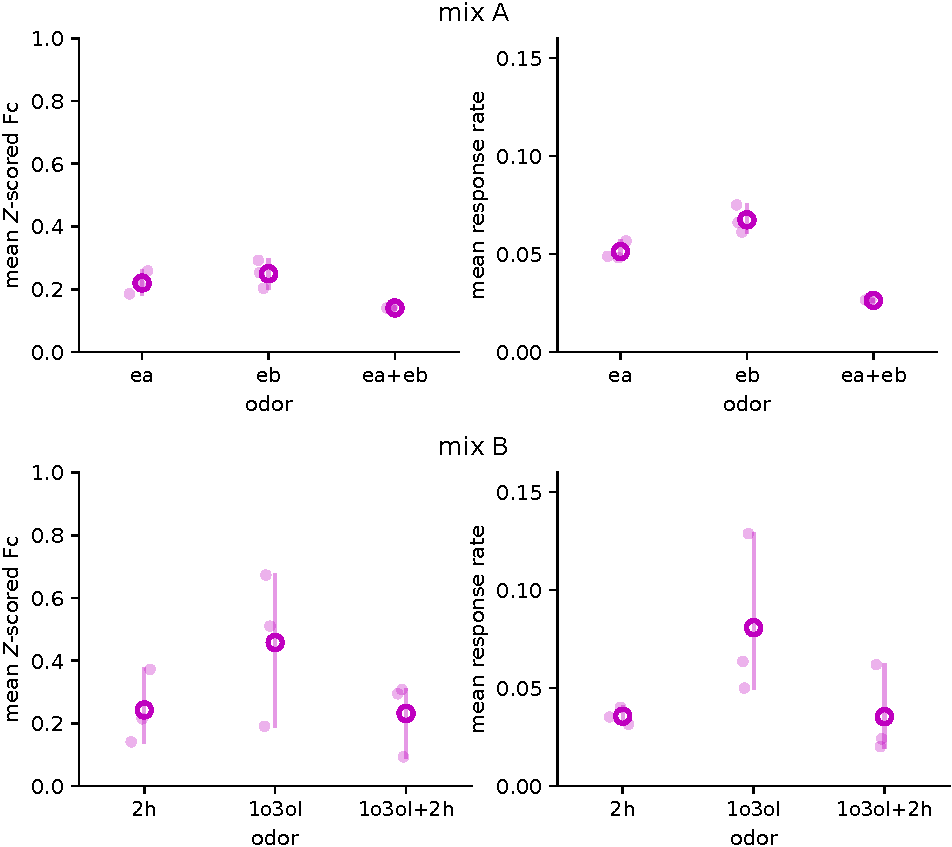
\includegraphics[width=\textwidth]{intensity_kc-only_binary}
% TODO make sure (at end) language is consistently either "binary" or "2-component".
% i suppose most/all plots currently have 2-component, but maybe ok to stick to "binary" in text still?
\mycaptionof{figure}{KC mean responses to binary mixtures}{%
Mean response amplitude, as measured by \KCRespStat values (left), and fraction of cells responding (``mean response rate''), after binarizing response amplitude with a threshold of $1.5$ (right).
All statistics were computed across all KC ROIs from Suite2p, without dropping cells responding subthreshold to all odors.
$n{=}3$ flies for each mix.
% TODO add terminology entry for ROIs ("region of interest")
% TODO terminology for Suite2p Fc?
}
\label{fig:intensity_kc-only_binary}
\end{longcapfigure}

\begin{longcapfigure}
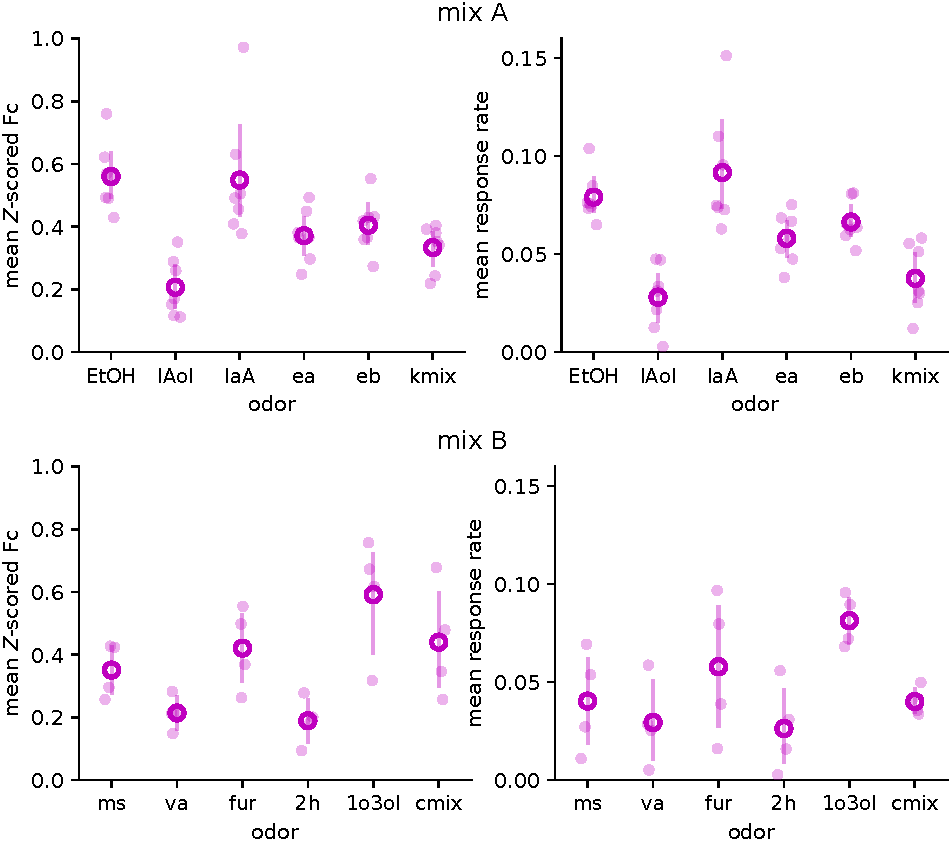
\includegraphics[width=\textwidth]{intensity_kc-only_5comp}
\mycaptionof{figure}{KC mean responses to five-component mixtures}{%
% TODO refer to a more standard methods section for this?
Mean response amplitude and mean response rate are as described in \cref{fig:intensity_kc-only_binary}.
For mix A and B, $n{=}7$ and $4$, respectively.
}
\label{fig:intensity_kc-only_5comp}
\end{longcapfigure}
% }

To investigate the consistency of mixture suppression across concentration scales, we also presented each binary mixture at additional 10x and 100x dilutions and observed that the trend of weaker mixture responses remained for both binary mixtures, measured in terms of both mean KC population activity and response rate (\crefwithbackref{fig:intensity_kc-only_pair-dilutions}).
The magnitude of mean response suppression may have started to decrease slightly in the 100x dilution, so it may not be invariant to larger changes in odor concentrations.

% Binary pair-dilution indensity figure
\begin{longcapfigure}
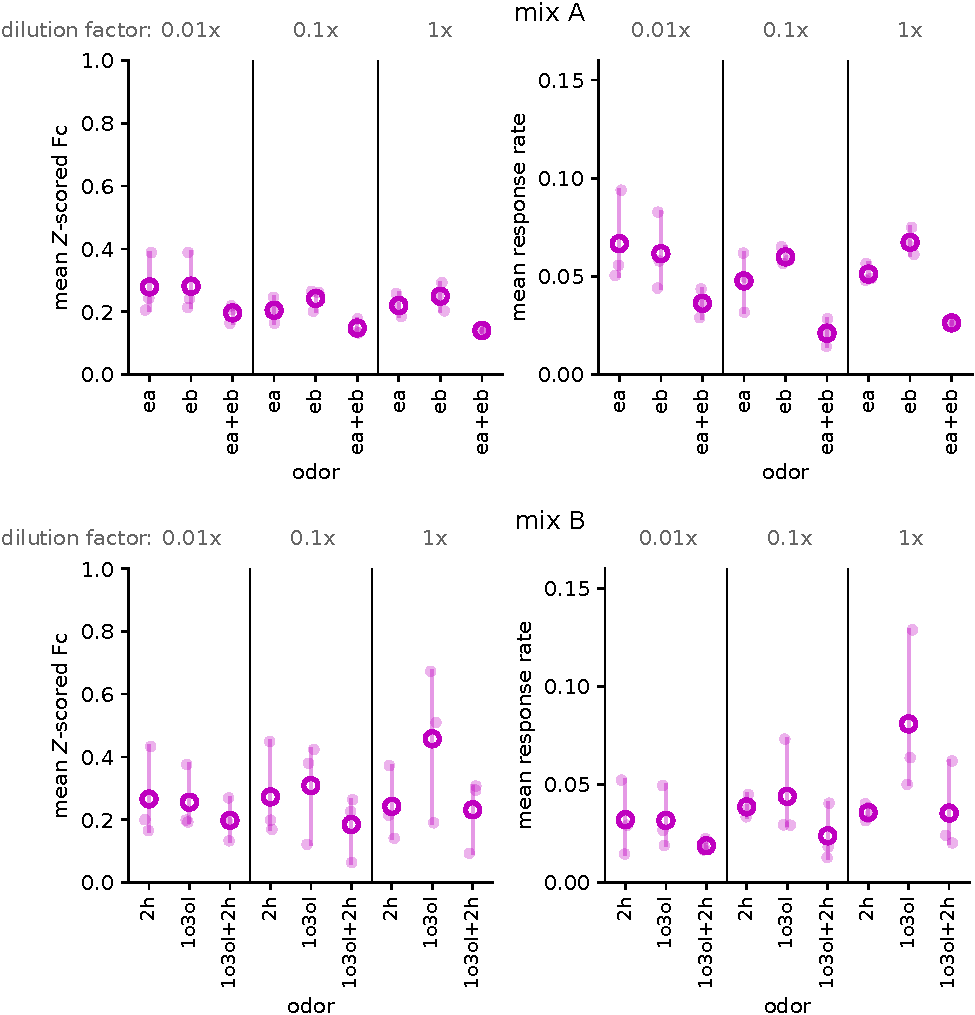
\includegraphics[width=\textwidth]{intensity_kc-only_pair-dilutions}
\mycaptionof{figure}{KC mean responses to three dilutions of 2-component mixtures}{%
Data for the 1x dilution case (right group in each panel) is the same data shown in \cref{fig:intensity_kc-only_binary}, with mean response amplitude/rate also as described there.
% TODO refer to a more standard methods section for the reference to reponse calculations?
}
\label{fig:intensity_kc-only_pair-dilutions}
\end{longcapfigure}
% TODO is it suprising at all that KC odor response intensity consistent across this range? existing data like that?
% (b/c ORN respresentation probably does broaden out a bit in general, ramping across 3 orders of magnitude)

% TODO delete?
% TODO TODO betty was confused about this. edit.
% "don't quite follow. what is the expectation? Is 1octen3ol an exception?"
%The mean responses to the components of both binary mixtures are also remarkably consistent across these dilutions, with a slight exception of 1-octen-3-ol in binary mix B, which has noticeably stronger responses at the highest concentration.
%To explore whether the change in response strength for 1-octen-3-ol can be explained largely by a population of cells that only respond at the highest concentration, we compare the clustered responses across the dilutions (\cref{fig:clust_hierarch_binary}), and there is a large cluster of strong responders at the 1x dilution that almost completely disappear by the 100x dilution.
%In contrast, the populations of cells responding to the other odors seem more consistent across dilutions.
%

% Per-odor distributions of KC and ORN intensity
% {
% TODO make smaller, to fit two per page, for comparison?
\begin{longcapfigure}
% TODO regen (or use?) logscaled version of full population counts (the left panels)?
\centering
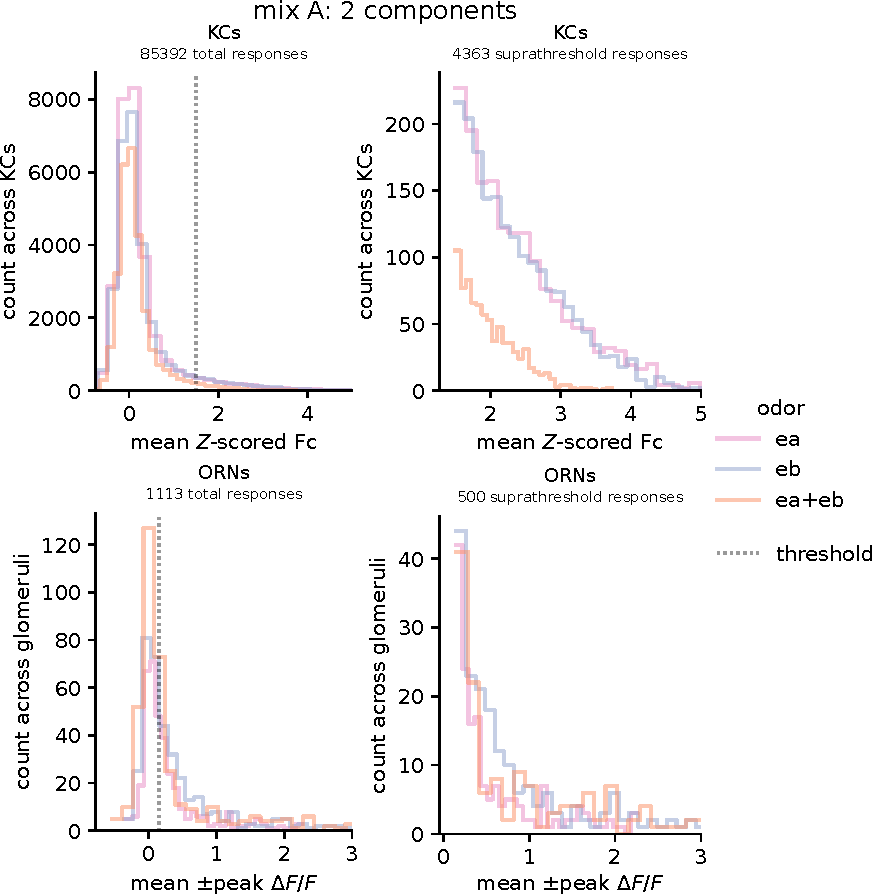
\includegraphics[width=\textwidth]{per-odor_counts_kiwi2_kc-orn}
\mycaptionof{figure}{Mix $A_2$ per-odor KC \& ORN response distributions}{%
% TODO TODO TODO justify this strict KC threshold (via application to megamat? via comparison of model response rates to the mean response rate we get with this? via sensitivity analysis, or at least trying one other response rate?) (i do have results supporting this now, by retrying w/ 0.8 thresh)
Left: distributions (across KCs or glomeruli) of all odor responses, with a vertical line indicating the response threshold used for the right panels (1.5 for KCs and 0.8 for ORNs).
Right: similar distributions, but now only including responses that are at or above threshold. This gives a sense both of the number of responses that pass threshold, and also how quickly they fall off at increasing response amplitudes.
}
\label{fig:per-odor_counts_kiwi2_kc-orn}
\end{longcapfigure}
% (this is last place the end fold mark worked, with one starting at all intro figs)

\begin{longcapfigure}
\centering
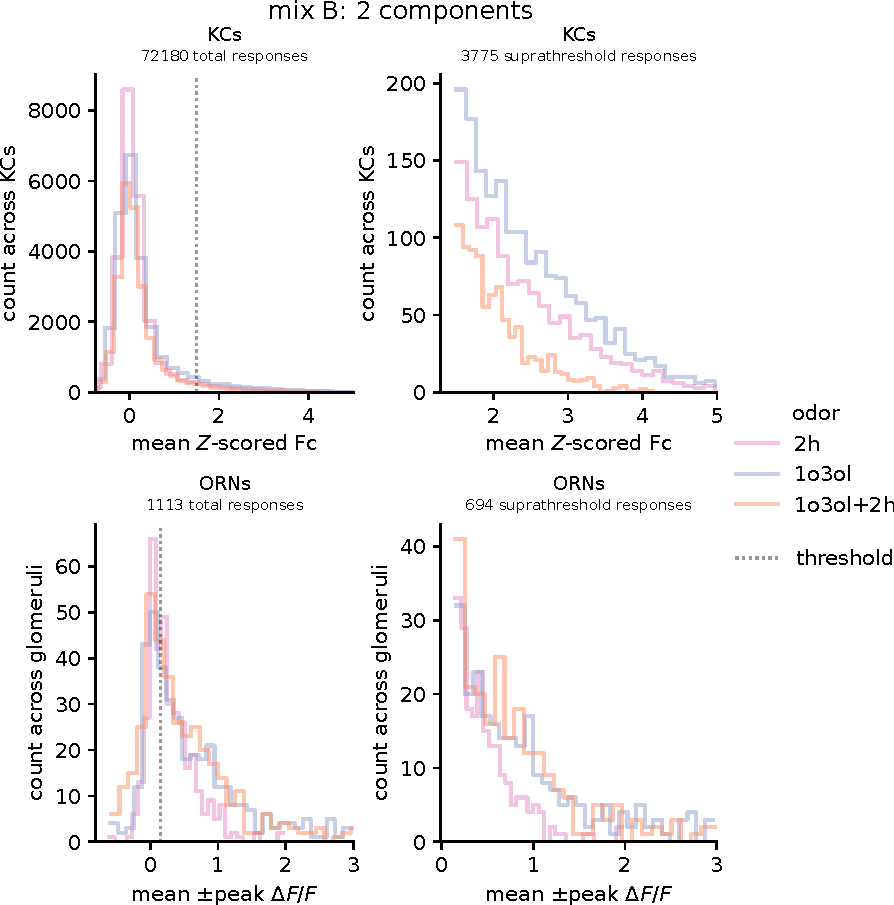
\includegraphics[width=\textwidth]{per-odor_counts_control2_kc-orn}
\mycaptionof{figure}{Mix $B_2$ per-odor KC \& ORN response distributions}{%
Organization and thresholds are as in \cref{fig:per-odor_counts_kiwi2_kc-orn}.
}
\label{fig:per-odor_counts_control2_kc-orn}
\end{longcapfigure}
% (end fold mark did NOT work here, when started before all intro KC figs)

\begin{longcapfigure}
\centering
% TODO want full textwidth here?
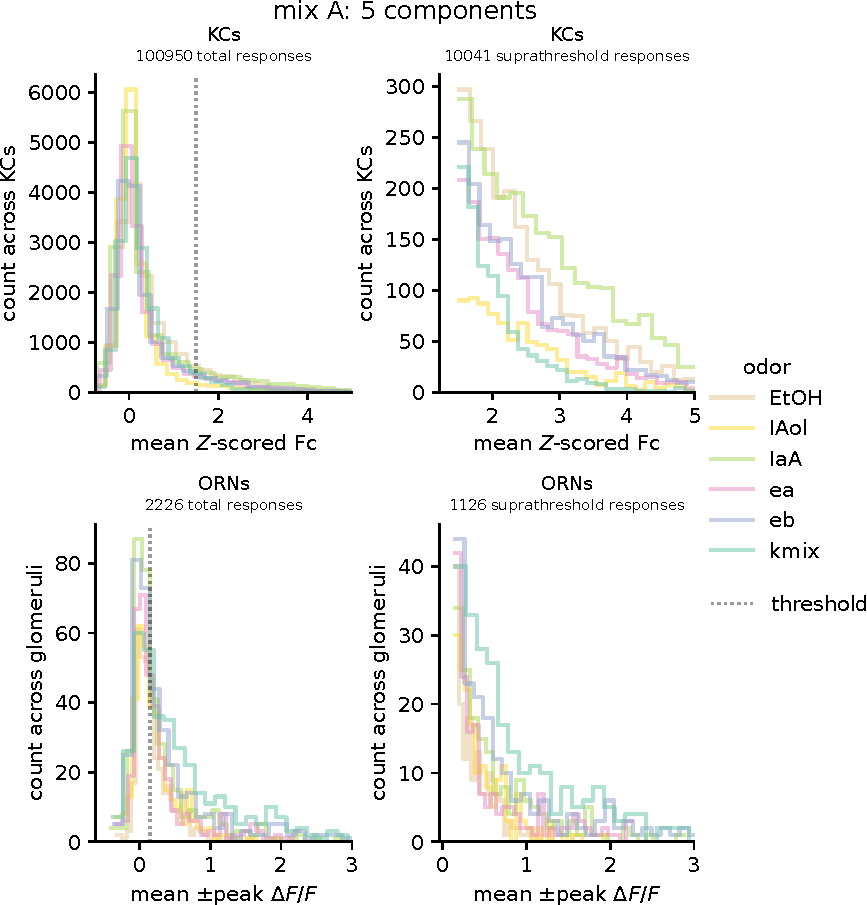
\includegraphics[width=\textwidth]{per-odor_counts_kiwi5_kc-orn}
\mycaptionof{figure}{Mix $A_5$ per-odor KC \& ORN response distributions}{%
% TODO want to restore manual ref here with "figure " prefix (\Cref would give "Figure " and \cref gives "fig. ")?
Organization and thresholds are as in \cref{fig:per-odor_counts_kiwi2_kc-orn}.
}
\label{fig:per-odor_counts_kiwi5_kc-orn}
\end{longcapfigure}

\begin{longcapfigure}
\centering
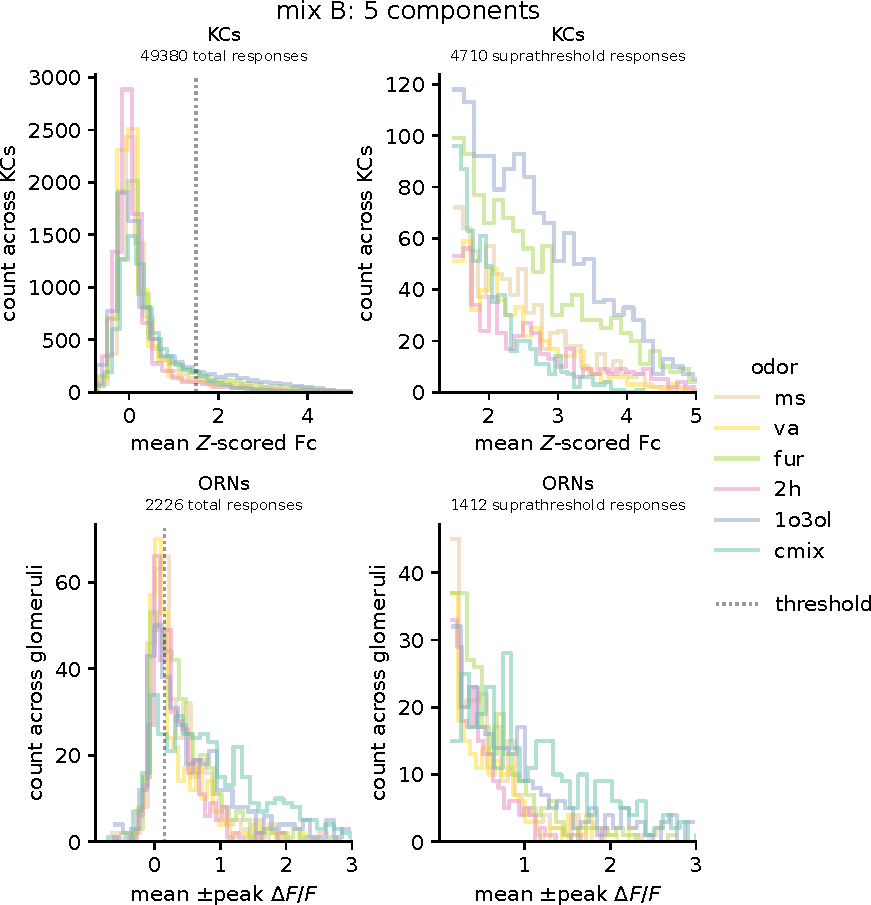
\includegraphics[width=\textwidth]{per-odor_counts_control5_kc-orn}
\mycaptionof{figure}{Mix $B_5$ per-odor KC \& ORN response distributions}{%
% TODO want to restore manual ref here with "figure " prefix (\Cref would give "Figure " and \cref gives "fig. ")?
Organization and thresholds are as in \cref{fig:per-odor_counts_kiwi2_kc-orn}.
}
\label{fig:per-odor_counts_control5_kc-orn}
\end{longcapfigure}
% }

Suppression of average mixture responses could be caused by either a change in response magnitude (among responding units) or a change in the number of responding units.
Both of these mechanisms seem to contribute for the binary mixtures, as each had a distribution of mix responses that showed fewer responding KCs and a weaker maximum response, when compared to the components (\crefwithbackref{fig:per-odor_counts_kiwi2_kc-orn} and \refwithbackref{fig:per-odor_counts_control2_kc-orn}; top).
The same two mechanisms also seem to play a role in the observed five-component mixture suppression, although it appeared that an even larger proportion of these mix-responses were weak (relative to component responses), compared to the proportion of weak mix-responses to the binary mixtures (\crefwithbackref{fig:per-odor_counts_kiwi5_kc-orn} and \refwithbackref{fig:per-odor_counts_control5_kc-orn}; top).
% TODO TODO clarify / delete B: "this needs clarification"
%The same two mechanisms also seem to play a role in the observed five-component mixture suppression, but now the mix response distributions also seem to fall off at lower intensities with a higher slope than for any of the component distributions (\cref{fig:per-odor_counts_kiwi5_kc-orn,fig:per-odor_counts_control5_kc-orn}).
%The more rapid falloff in five-component mix response distributions may indicate that these mixtures see more suppression coming from a change in the response magnitude (within responders), rather than strictly a change in the number of cells responding.

% TODO keep?
%The same distributions computed on the ORN data show that the distributions of component and mixture responses are much more similar across all mixtures, both in terms of the number of responding glomeruli and in their response strengths.
%Both five-component mixtures seem to show some combination of more responding glomeruli, as well as a rightward shift to higher response intensities, for the ORN mix response distributions.

% TODO TODO add back somewhere? delete?
%The impression of the KC data in these figures holds across a wide range of KC thresholds, from the relatively stringent 1.5 (used for all mix A \& B KC data throughout this chapter), all the way down to the relatively permissive 0.8 (see Methods for justification of this range).

\subsection{Most responsive KCs are component-selective, with little mix response}
We next sought to better understand the response features at the level of individual KCs that give rise to mixture suppression observed on a population level.
We investigated the tuning profiles of individual KCs to mixtures and their constituent components, and characterized the distribution of these response classes across the whole population of KCs in a given mushroom body.
% TODO TODO de-dedupe some of these questions w/ above (prob deleting above)
Do cells that respond to the components also respond to the mix, though perhaps with a weaker amplitude?
Do populations of cells tend to respond to particular combinations of components?
If there are cells responding selectively to any of the mixtures, does the size of the mix-selective population change depending on some properties of the odor mixture?

We binarized each cell's response vector across odors (response threshold of 1.5) and sorted them by 1) whether or not they responded to the mix; 2) to how many components they responded to; and 3) to which component they responded to maximally (see Methods).
We call the groups produced by this approach ``response classes''.\nomenclature{response class}{a summary of the response of a neural unit (neuron / glomerulus) to a mixture and its components, which starts by binarizing the responses and then differentiates tuning based on whether the unit responds to the mix, how many components it responds to, and which component it responds the most to.}
We grouped each KC into one of these response classes and examined the total fraction of ROIs occupying each response class (\crefwithbackref{fig:response-class-means_kc_binary} and \refwithbackref{fig:response-class-means_kc_5comp}; \crefwithbackref{table:kc_resp_types}).
We observed that KC tuning profiles and their distribution were remarkably stereotyped across flies, as evidenced by the consistent representation of flies (colors) in every response class.
This response consistency is robust even though each mushroom body is probabilistically wired with a unique PN-KC connection matrix.
The largest class of cells was consistently those that responded to no odors in our stimulus panel, ranging from 73.1\% to 88.5\%, reflecting the sparse response rate in KCs.
% TODO move to methods? first paragraph?
%The overall character of these response class distributions (as well as the mean responses within them) do not seem to depend much on choice of KC response threshold, even as low as 0.8 (data not shown).

% KC response class means and counts
% {
\begin{longcapfigure}
\centering
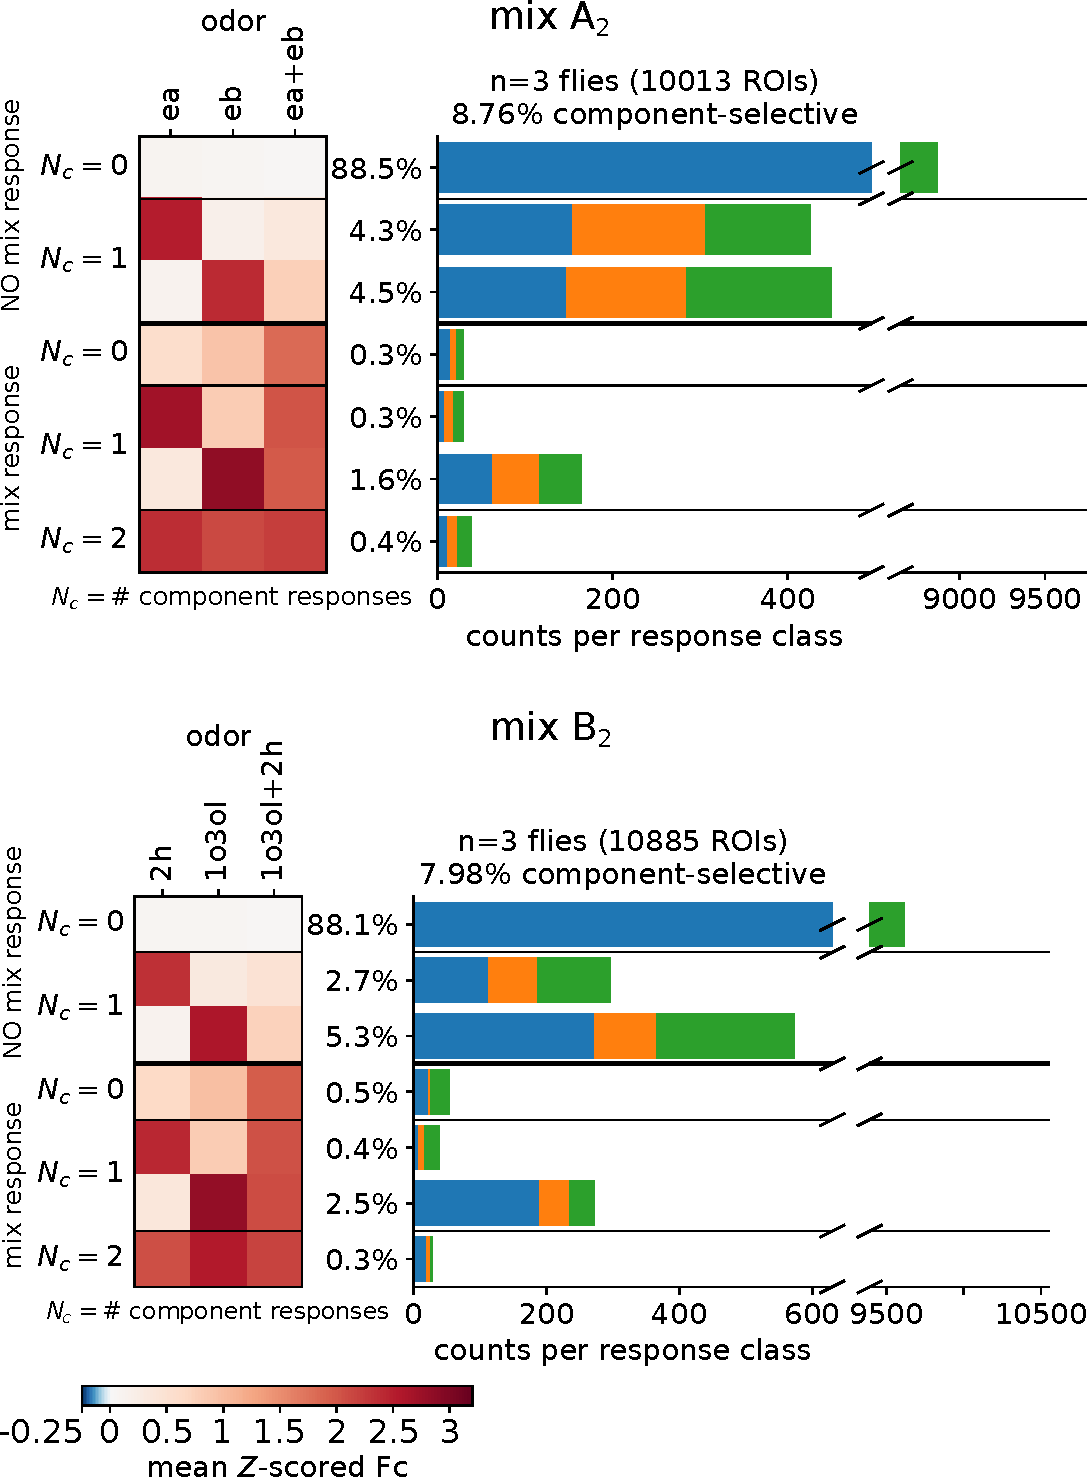
\includegraphics[width=\textwidth]{response-class-means_kc_binary}
\mycaptionof{figure}{KC 2-component mix response class means and counts}{%
Left: mean responses across all KCs within a response class.

Right: counts of this response class, across KCs from all flies, where the denominator is the total number of ROIs detected (rather than the filtered subset used for most analyses; see \cref{table:sample_sizes}).

Different colors in right panel bars correspond to different flies.
% TODO move to methods (+ delete everywhere)
%Classes containing less than 0.25\% of ROIs have been excluded, so percentages may not sum to 100.
% TODO delete text (already in table) refer to table!
%Mix-responsive fractions are 2.63\% for mix A and 3.64\% for mix B.
}
\label{fig:response-class-means_kc_binary}
\end{longcapfigure}

\begin{longcapfigure}
\centering
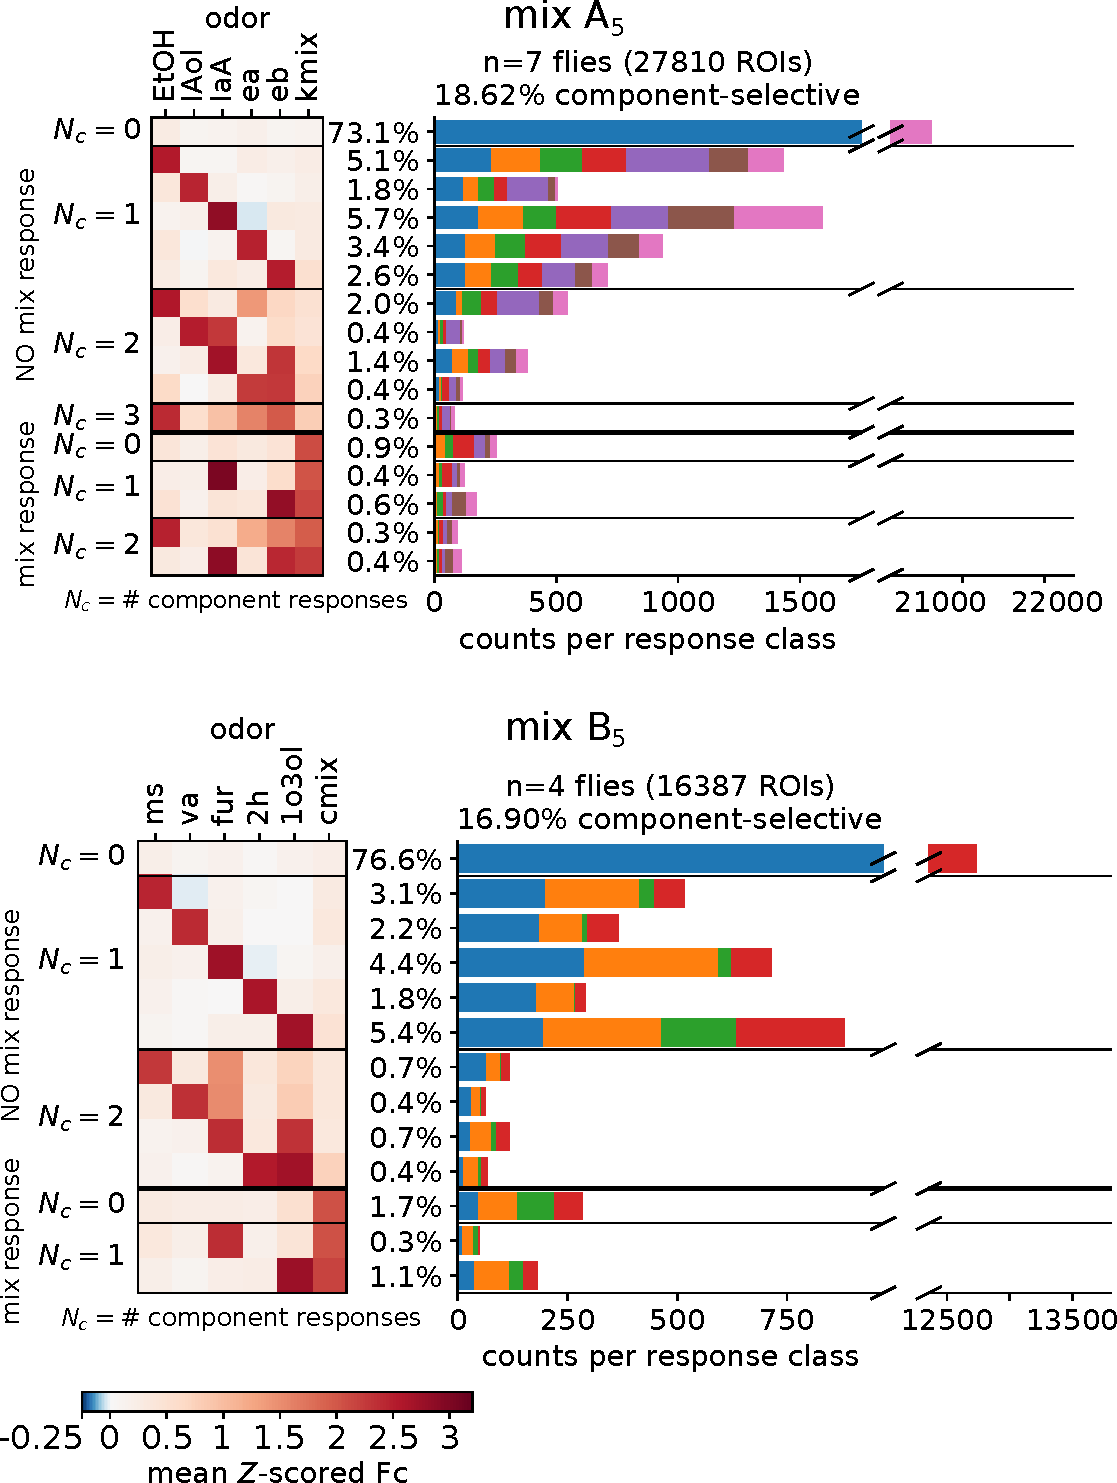
\includegraphics[width=\textwidth]{response-class-means_kc_5comp}
\mycaptionof{figure}{KC five-component mix response class means and counts}{%
Similar to \cref{fig:response-class-means_kc_binary}.
Colors again correspond to different flies, but these are all different flies from the binary experiments (colors are not shared across mix A \& B for the KC dataset).
% TODO move to methods (+ delete everywhere)
%Classes containing less than 0.25\% of ROIs have been excluded, so percentages may not sum to 100.
% TODO delete text (already in table) refer to table!
%Mix-responsive fractions are 2.74\% for mix A and 3.14\% for mix B.
}
\label{fig:response-class-means_kc_5comp}
\end{longcapfigure}
% }

We expected that there might be some KCs that responded exclusively to the mix (and not to any of its components); perhaps because a KC samples two glomeruli (each selective to one component's ORN representation), where neither input is strong enough alone to drive the KC to spike, and both inputs need to be active together.
To our surprise, we observed no cells that responded exclusively to either binary mixture, and only small populations of cells (\qtyrange{0.9}{1.7}{\percent}) selective for either of the five-component mixtures A or B.
Despite their small size, these mix-selective populations were present in every fly.
The slightly larger population of mix-selective KCs for mix B compared to mix A might reflect the comparatively greater chemical diversity of mix B, reflected in the more diverse ORN representations driven by the components of mix B (seen in the decreased correlation among mix B components compared to mix A in \crefwithbackref{fig:orn_corrs}).

After the non-responders, the majority of the remaining KCs responded selectively to single odors, and \textit{not} to the mix, a type of response class we call ``component-selective''.
This fraction of KCs ranged from \textasciitilde\qtyrange{8}{9}{\percent} in the binary mixtures to \textasciitilde\qtyrange{17}{19}{\percent} in the five-component mixtures (\cref{table:kc_resp_types}).
% TODO TODO in discussion, talk about how we don't see same segmenting behavior as prominent in laurent paper
% (that responsd the to components regardless of whether alone or which mix they are in)
The remaining fraction of cells, in response classes other than non-responders or component-selective cells, was less than 10\% in all cases, and less than 5\% for all but five-component mix A.
% TODO TODO move to discussion (/delete)
%It is interesting that the KCs are so selective for single components, as the ORNs they ultimately receive input from overwhelming respond to multiple odors (\crefwithbackref{fig:frac_response_class_kc-orn}).

% Fraction of KCs in different response classes
\begin{longcaptable}
% TODO TODO TODO also include # responders to each mix, either in this table or elsewhere?
% TODO TODO TODO and/or (only?) report percentages wrt responding fraction?
% (or fraction responding to component in some cases?)
\centering
% (i liked tabular better w/ everything else as-is. tabularx still wasn't bottom justifying the NComps and Response Type multirow columns, and other things were uglier)
\begin{tabular}{crcc}
% TODO maybe add the vertical rules for this table? "|" characters in spec above
\multirowthead{2}{\thead{\NComps}} &
\multirowthead{2}{\thead{Response Type}} &
% TODO any reason to use \cmidrule instead of \cline?
\multicolumn{2}{c}{\thead{\% of ROIs}}\\ \cline{3-4}
  & & \thead{Mix A} & \thead{Mix B}\\
\midrule
\multirow{4}{*}{5}
& non-responding & 73.1\% & 76.6\%\\
& component-selective & 18.6\% & 16.9\%\\
& mix-responsive & 2.7\% & 3.1\%\\
& mix-selective & 0.9\% & 1.7\%\\
\hline
\multirow{4}{*}{2}
& non-responding & 88.5\% & 88.1\%\\
& component-selective & 8.8\% & 8.0\%\\
& mix-responsive & 2.6\% & 3.6\%\\
& mix-selective & 0.3\% & 0.5\%\\
\bottomrule
\end{tabular}
\mycaptionof{table}{KC response class percentages}{%
The mix-responsive percentage includes the mix-selective cells, as well as those that also respond to components.
}
\label{table:kc_resp_types}
\index{tables}
\end{longcaptable}

\subsection{More KC mixture suppression in five-component than binary mixtures}
% TODO move to discusssion
%From the previous section, it became clear that much of the hints of mixture suppression we saw in the average response statistics and the per-odor response distributions can be explained by the majority of the KCs responding to single components, and by the fact that the mix responses that do exist tend to be weaker than typical component responses.
We next asked how the extent of KC mixture suppression varied across the number of components and the particular mixtures.
Do mixtures with more components tend to have their response suppressed more than mixtures with fewer components?
%Do mixtures with particular composition, or particular types of components, tend to see more suppression?

% TODO TODO TODO move to methods??
% NOTE: \, = "thin space" (without it the set notation would be crowded)
% \[ \] surrounds an equation we want centered
For the purposes of this chapter, we define mixture suppression per KC (or glomerulus) as: \[ \text{response}_{mix} - \underset{c \, \in \, \text{components}}\max \, \text{response}_c \]

% TODO also say something about "values around 0" -> "hypoadditivity"?
where negative values should be interpreted as mixture suppression, and positive values as synergy.
% TODO move to methods
%All analyses that follow in this chapter, which compute mixture suppression per coding unit, first restrict the units to those that respond (above threshold) to at least one odor (whether component or the mix).

% TODO actually link to relevant methods section
% TODO move this to methods?
%Note that my definition of mixture suppression contrasts with another common definition used for mixture suppression in existing literature (not always calculated within individual coding units), which instead compares the mix response to the sum of the component responses (and is sometimes referred to as "linearity").
%See Methods for more details on why the calculation above may be more appropriate.
% END PART TO MOVE TO METHODS

% Distributions of mixture suppression for 2/5-component mix A/B (KCs vs ORNs)
\begin{longcapfigure}
\centering
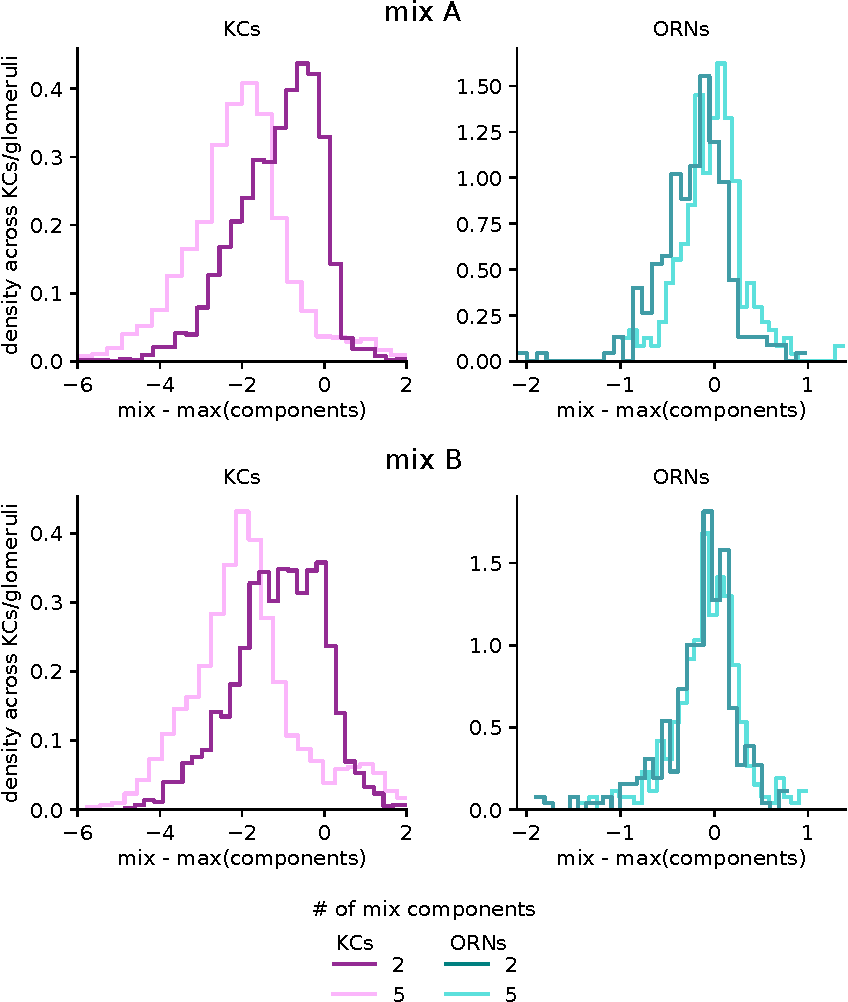
\includegraphics[width=\textwidth]{mixsupp_dists_kc-orn}
% TODO TODO regenerate at least KC side with fixed xlim (and maybe draw dotted vertical lines at means?), to make comparing across rows more sensible
\mycaptionof{figure}{Distributions of KC and ORN mix suppression}{%
Density of mixture suppression across KCs (left) or glomeruli (right), for both mix A (top) and mix B (bottom).
Different line colors indicate the number of components in that variant of the corresponding mixture.
Mixture suppression was computed only within cells that responded (above threshold) to at least one odor.
}
\label{fig:mixsupp_dists_kc-orn}
\end{longcapfigure}

When comparing KC mixture suppression distributions for the two- \& five-component variants of each mixture, it was clear that there was more mixture suppression to the five-component mixtures (\crefwithbackref{fig:mixsupp_dists_kc-orn}; left).
Within mixtures of a given number of components, the mixture suppression distributions seemed similar, indicating the additional complexity of the mixtures with more components is important to their ability to recruit more KC mixture suppression.
% TODO delete?
%There may also be small lobes of positive mix suppression in both of the five-component KC distributions, although more prominent for mix B, which is consistent with the higher fraction of the mix-selective response class we saw for this mixture earlier.
% TODO TODO TODO move to ORN section
%The distributions of mixture suppression across glomeruli once again indicate there are not significant populations exhibiting meaningful mixture suppression or synergy, at least for these particular mixtures.

% Distributions of KC binary mix suppression across pair dilutions
\begin{longcapfigure}
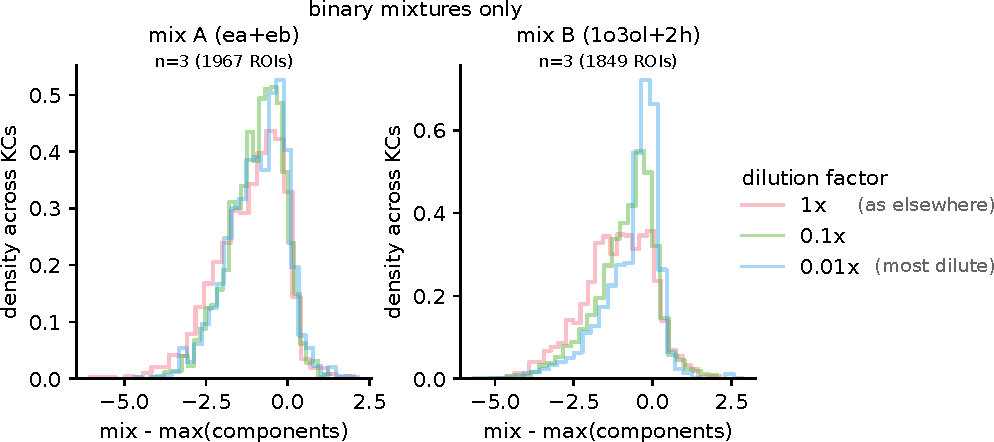
\includegraphics[width=\textwidth]{mixsupp_dists_kc-only_pair-dilutions}
% TODO remove the explicit listing of the two odors in the binary mixture in titles for this fig, for consistency
\mycaptionof{figure}{Distributions of KC mix suppression, for three dilutions of the binary mix A \& B}{%
See \cref{fig:clust_hierarch_binary} for more details on the stimuli.
}
\label{fig:mixsupp_dists_pair-dilutions}
\end{longcapfigure}

We briefly returned to analyzing the dilutions of the binary mixtures, to ask whether the degree of mixture suppression seemed to vary across the concentration scales (\crefwithbackref{fig:mixsupp_dists_pair-dilutions}).
% TODO move expectation to discussion?
We might expect that as the amount of peripheral drive decreases, there should be less feedback inhibition from the APL, resulting in less mixture suppression.
Mix B (right) may have slightly exhibited this trend: as the mixture got more dilute, there were more cells with lower mixture suppression.
For mix A, however, the distributions seemed to suggest that this mixture response was consistently suppressed, across these dilutions that span three orders of magnitude.
% TODO move to discussion?
%This could be simply because the component representations are more stable (remaining more consistently intense) at the ORN level for the components of mix A, relative to mix B, but would require the same experiment to be done in the ORNs to confirm.

% TODO maybe this one can stay a subsubsection?
\subsection{Binary mixtures of weakly-activating odors drive less KC suppression}
Despite sweeping the previous binary mixtures across a range of concentrations, the components of those mixtures likely still evoke reasonably broad and strong activity in the AL.
Over the course of developing our odor-based method of glomerular identification, we identified several odors known to activate only a small number of glomeruli  (``weakly-activating''\footnotemark[1]{}).
We constructed an additional set of binary mixtures, now using combinations of these weakly-activating odors, to see whether the extent of mixture suppression in the KCs depends on the strength with which the components activate the ORNs.
%It should be noted that there it can be somewhat tricky to disentangle effects driven by overall activation across all ORNs (``strength'' / ``intensity'') from effects driven by how narrow or broad the ORN tuning pattern is, since many odors that reliably drive only weak ORN activity are also somewhat selectively (``narrowly'') activate only a small number of glomeruli.
%With that in mind, I will refer to the odors in this new set as ``weak'' or ``weakly-activating'' for convenience.
For these experiments we chose the following components: 2-heptanone, farnesol, and methyl acetate, all at concentrations low enough to be weakly-activating (see \cref{table:mix_odors}).

\footnotetext[1]{It can be tricky to disentangle whether effects are driven by ORN activation magnitude vs. breadth, since many odors that reliably drive only weak ORN activity also selectively activate a small number of glomeruli.}

% weak binaries figures (clustering, intensity, and mix suppression distributions)
% {
\begin{longcapfigure}
\includegraphics[height=0.8\textheight]{clust_hierarch_diag-binaries}
\mycaptionof{figure}{Clustered KC responses to binary mixtures of weak odors}{%
% TODO move to methods -> ref here -> make full height again?
% TODO TODO change title to only say n=12 once, since all odors are measured in all flies
As before, only cells responding to at least one component or the mixture are shown.
Unlike other KC analyses, this dataset considers KCs as responding to an odor if they respond above-threshold on at least 3 of 4 trials (more trials than the 3 for the other datasets), with a lower \KCRespStat threshold of 1.0.
All odors were measured in each of the 12 flies, and all odors (including components) were only measured in one set of trials, thus the 2h/ma/farn data in each of the three subplots are a reanalyzed version of the same data, to compare within each mixture.
}
\label{fig:clust_diag-binaries}
\end{longcapfigure}

\begin{longcapfigure}
\centering
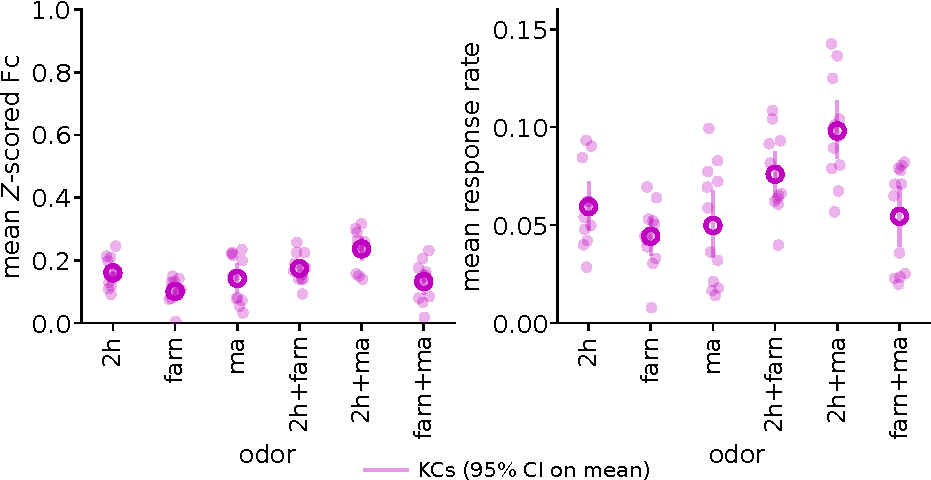
\includegraphics[width=\textwidth]{intensity_diag-binaries_kc-only}
\mycaptionof{figure}{KC average responses to binary mixtures of weakly-activating odors}{%
% TODO also refer to either methods or first KC-only figure for description of top statistics
KC response calling (for right panel) is as described in \cref{fig:clust_diag-binaries}.
}
\label{fig:intensity_diag-binaries_kc-only}
\end{longcapfigure}

\begin{longcapfigure}
\centering
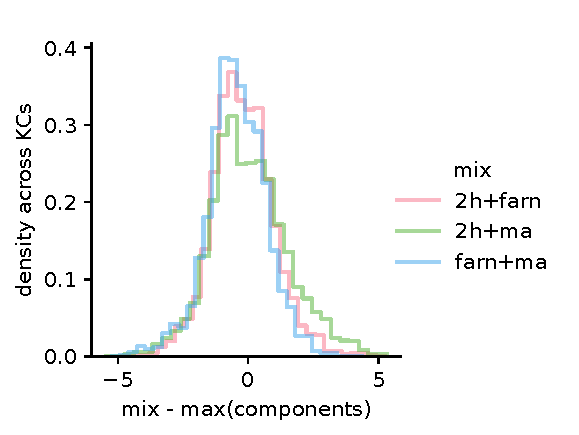
\includegraphics[height=3in]{mixsupp_dists_diag-binaries_kc-only_hue}
\mycaptionof{figure}{Distributions of KC mixture suppression to binary mixtures of weakly-activating odors}{%
% TODO add note on statistic it's computed on (and elsewhere? consolidate?)
Distributions are all centered around 0, without much bias towards negative values (increased mixture suppression). Similar distributions for each of these three mixtures. $n$=12 flies.
% TODO what's standard format papers use to put N in caption? copy that and be consistent
}
\label{fig:mixsupp_dists_diag-binaries_kc-only}
\end{longcapfigure}
% }

Clustered responses for these three mixtures can be seen in \Crefwithbackref{fig:clust_diag-binaries}.
We saw that these stimuli did indeed activate the KCs more weakly (compare left of \crefwithbackref{fig:intensity_diag-binaries_kc-only} with previous \cref{fig:intensity_kc-only_binary,fig:intensity_kc-only_5comp}).
% TODO still mention somewhat?
%From our various ORN datasets, we also know that the ORN responses are also weaker for these stimuli, compare to the prior two mixtures.
As expected, these odors that drive drastically less ORN and KC input also produced less KC suppression of their mixtures (\crefwithbackref{fig:mixsupp_dists_diag-binaries_kc-only}).

% TODO TODO rewrite these two sentences
%Knowing that these stimuli drive less activity, my expectation would be that these mixtures should exhibit less mixture suppression than any of the mixtures we have analyzed so far.
%Although the mixture suppression distributions are much more centered on 0 (as expected), they all still have a leftward bias indicating some KCs with their mix responses suppressed (\crefwithbackref{fig:mixsupp_dists_diag-binaries_kc-only}), and such KCs can also be seen in the clustering.

% TODO can i easily test if endfloat is disabled? maybe by setting disable by some other conditional i test (or some other variable i set in the same conditionals)?
% (maybe i only want to clearpage or whatever if not using endfloat?)
%\processdelayedfloats
%\clearpage

% TODO should there be a separate mini-discussion just in the descriptive part? meh

% TODO TODO do i actually anywhere above say that 2-component mix A has more suppression than mix B? b/c the data (avg mixsupp plot, as well as mixsupp distributions) don't really bear that out, so need to delete (maybe i just thought that would be the case from looking at intensity plots?)

\subsection{KC mixture suppression is not largely inherited from the ORNs}

% TODO move the odor-odor correlations to supplement? (if i'm only gonna discuss in discussion...?)
% ORN figures (mean responses & odor-odor correlations)
% {
\begin{longcapfigure}
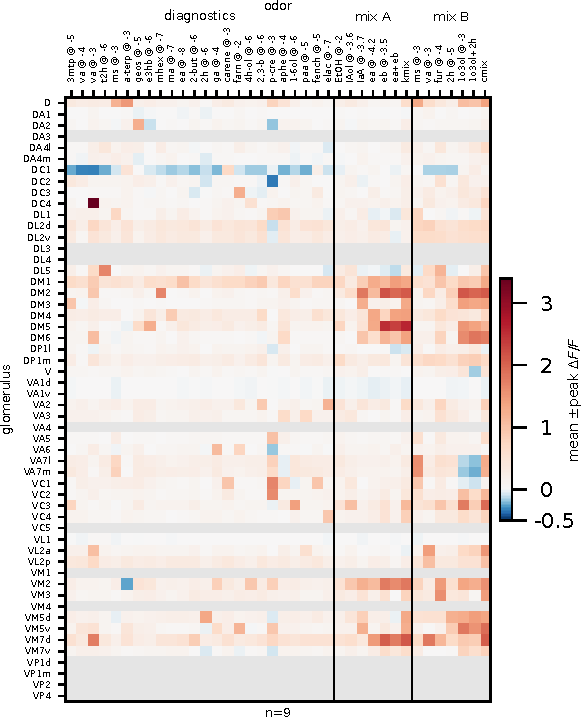
\includegraphics[width=\textwidth]{orn_mean_responses}
\mycaptionof{figure}{Per-glomerulus mean ORN responses to odors in mix A \& B}{%
% TODO get methods details for sampling rate
% TODO more details about glomeruli sampling (maybe just make and refer to N plot)
Responses (\ORNRespStat) were defined as the peak (either positive or negative, whichever has the highest absolute value) response within the 2 volumes (\textasciitilde\qty{2}{\second} at usual volumetric sampling rate), with the sign preserved.
This value was then averaged over the three trials, and over all of the flies with that glomerulus identified (see \crefwithbackref{fig:orn_stddev_and_n} for description of sampling of each glomerulus).
Left: responses to the ``diagnostic''\nomenclature{diagnostic odor}{an odor used to evoke activity in known glomeruli, typically aiming to activate one glomerulus in particular.
Used to assist in defining ROIs for and identifying glomeruli
} odors used to assist in identifying and segmenting the glomeruli.
The same 9 flies have data from each of these three panels: diagnostics, mix A, \& mix B.
}
\label{fig:orn_mean_responses}
\end{longcapfigure}

\begin{longcapfigure}
\centering
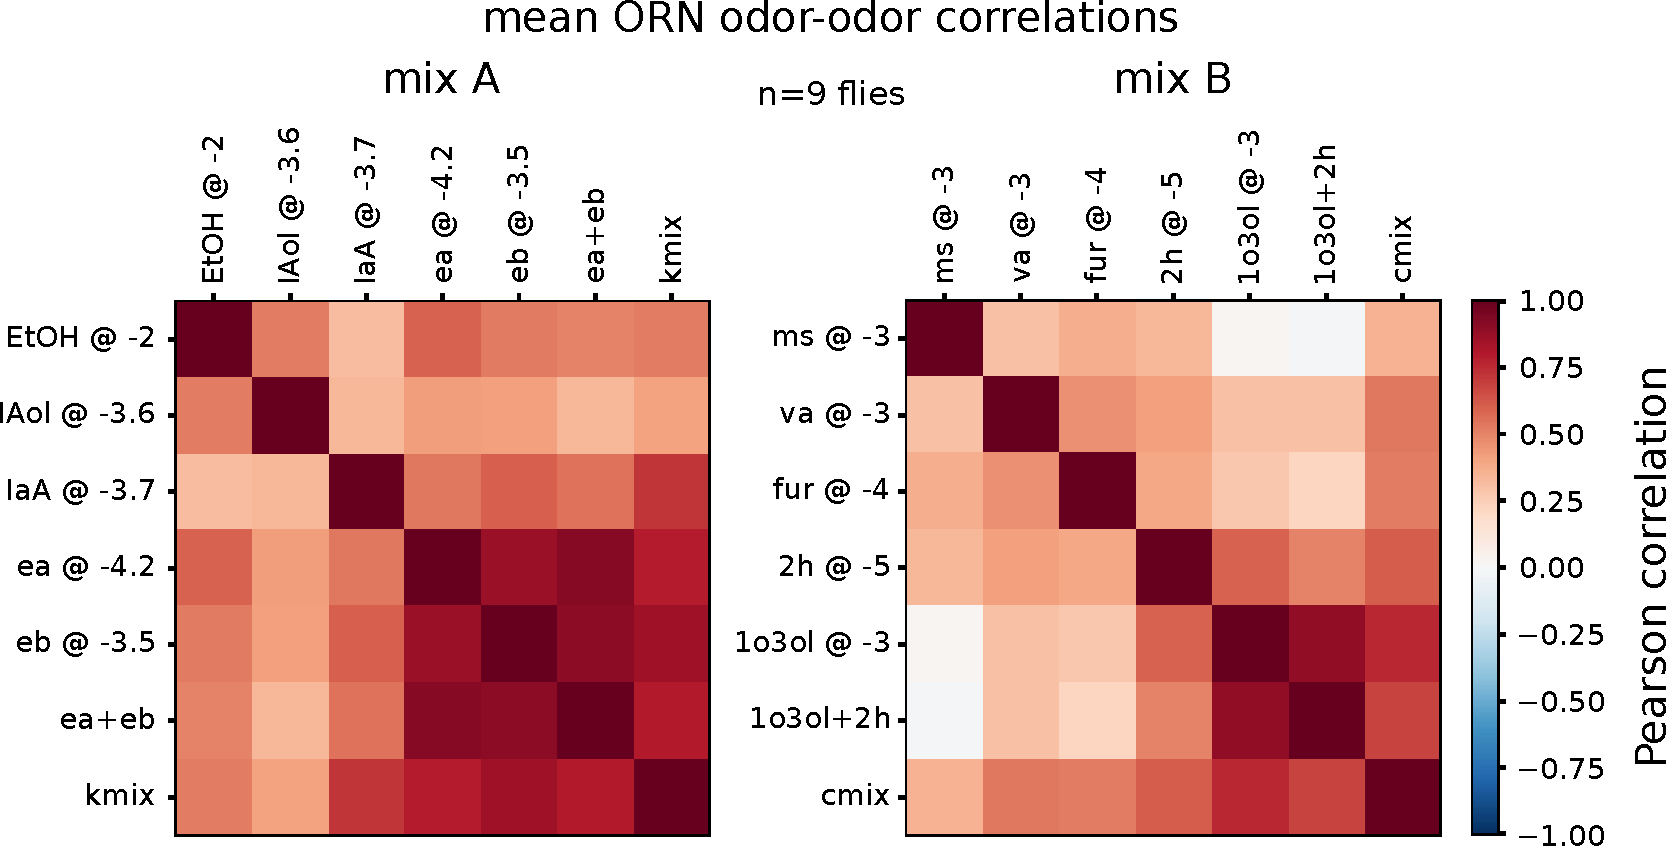
\includegraphics[width=4in]{orn_corrs}
\mycaptionof{figure}{ORN correlations between odors within mix A \& B}{%
Odor-odor Pearson correlations were computed within each fly (across the glomeruli identified in the particular fly), and then the correlation matrices were averaged across flies.
}
\label{fig:orn_corrs}
\end{longcapfigure}
% }

% TODO TODO use? (/delete) (move to supplement?)
% KC vs ORN response class summary
\begin{longcapfigure}
\centering
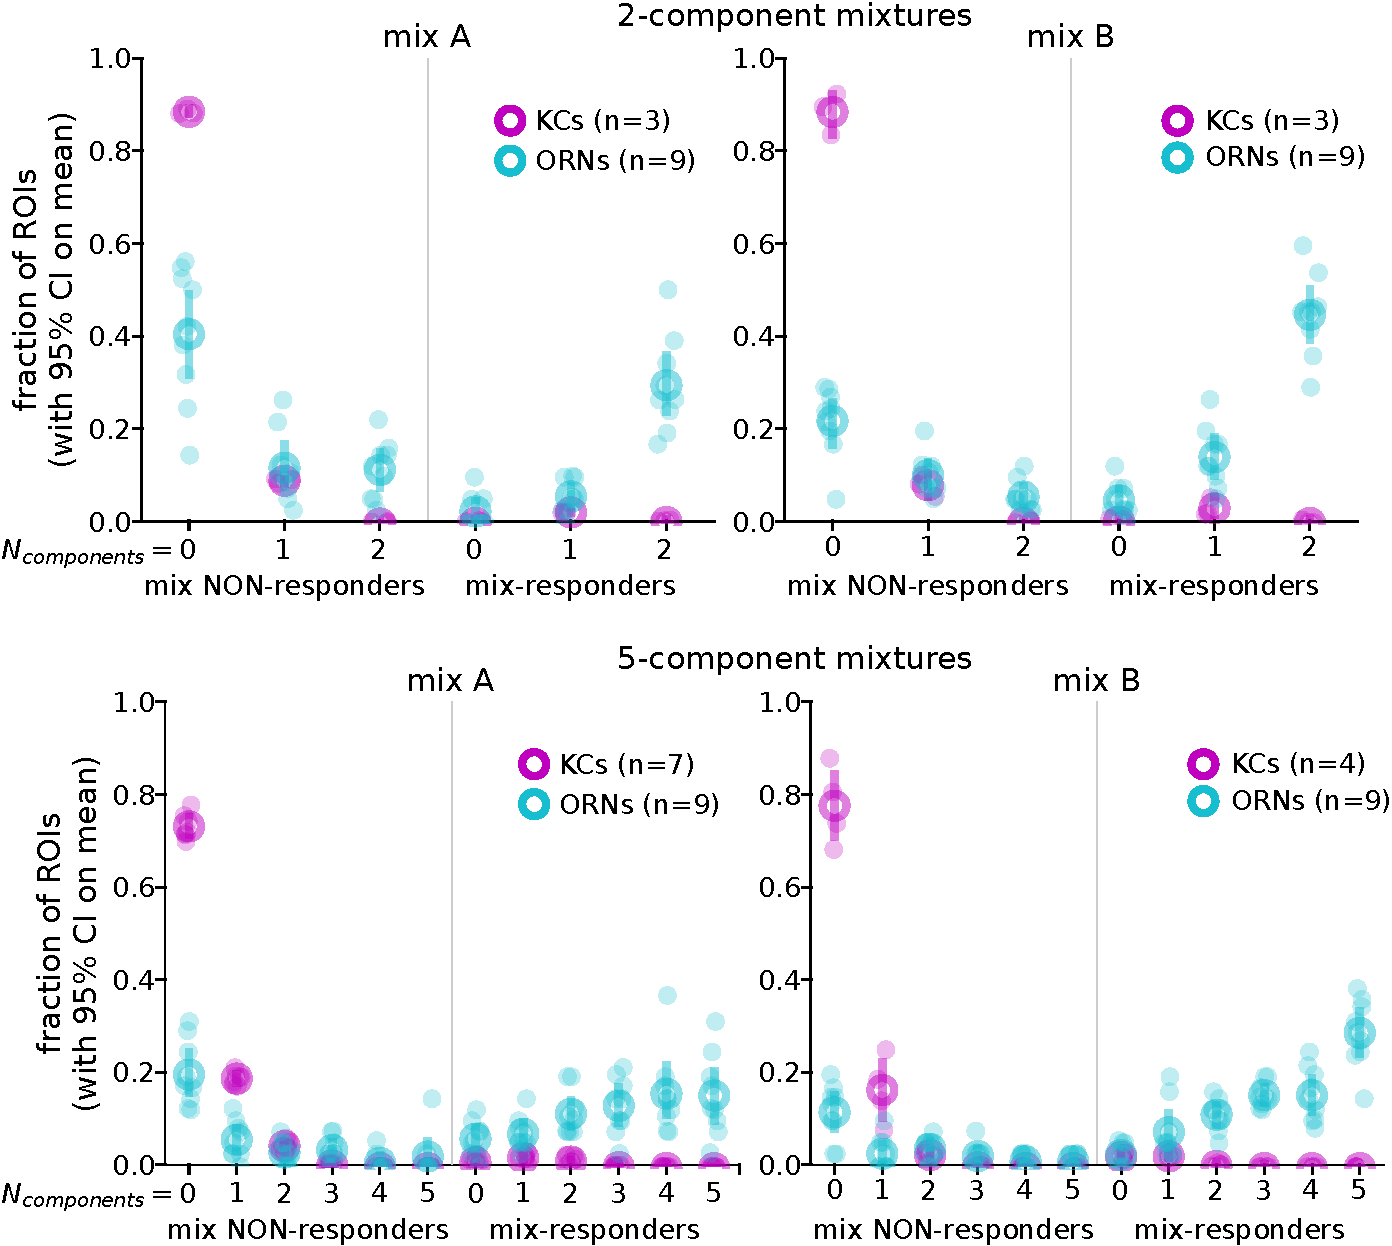
\includegraphics[width=\textwidth]{frac_response_class_kc-orn}
% TODO better name in this caption than "response class summary"?
\mycaptionof{figure}{KC \& ORN response class summary}{%
Response classes grouped by whether they are mix-responsive and their number of component responses, ignoring which component had the maximal response.\\
ORN response threshold was chosen as 0.8 \DeltaFOverF.
Breakdown of the ORN response classes can be seen in \crefwithbackref{fig:response-class-means_orn_binary} and \crefwithbackref{fig:response-class-means_orn_5comp}.
}
\label{fig:frac_response_class_kc-orn}
\end{longcapfigure}

With many studies demonstrating receptor-level antagonism between odors, and other effects that could support mixture suppression in the periphery, we asked to what extent mixture suppression in the KCs seems inherited from effects in the ORNs.
We recorded ORN axon terminals in the AL glomeruli, with the same two- \& five-component mixture panels, in 9 flies (\crefwithbackref{fig:orn_mean_responses}).
% TODO TODO move near sample size table?
%The per-glomerulus mean responses are in \crefwithbackref{fig:orn_mean_responses}, with the standard deviation (across flies) and the number of times each glomerulus was identified per fly in \crefwithbackref{fig:orn_stddev_and_n}.
%
Inhibition, which could represent either inverse agonism or inhibition onto ORN axon terminals, did not seem to be a prominent feature of the responses to the odors in these mixtures, although there may have been slightly more in the responses to the mix B components (which are less appetitive overall).

% TODO save for discussion / delete
%Isoamyl acetate is also a component of many appetitive natural mixtures, and is also relatively more activating in this KC dataset, but the effect is less dramatic than for ethanol.
%It would be interesting if certain categories of odors are able to recruit more KC activity than expected from ORN responses, perhaps through a mechanism that involves additional feedback inhibition scaled through activity of the LH.

Unlike in the KCs, the mean activation of ORNs to the mixtures was not weaker than to any components (\crefwithbackref{fig:intensity_orn}).
To compare the magnitude of this suppression between KCs and ORNs, we separately normalized each dataset and showed that KC population responses to all mixtures were suppressed (below the population responses to any component) more than in ORNs (\crefwithbackref{fig:intensity_orn-vs-kc}).
In contrast to KCs, most responsive glomeruli responded to the mixtures, and there were very few component-selective glomeruli (\crefwithbackref{fig:frac_response_class_kc-orn}).
Glomeruli exhibited little, if any, mixture suppression to any of our mixtures (\cref{fig:mixsupp_dists_kc-orn}; right).
Comparing this with the much more dramatic KC mixture suppression to all of the mixtures, it does not seem that much of the KC suppression can be explained by effects visible in the ORN axon terminals.

% betty said on this:
% "This is not really related to mixture suppression. The odor-specific gain on certain odors is a separate observation, and since each ocmponent is measured in the KC experimentally, the suppression analysis takes it into account."
%\iffalse
%When comparing the ORN and KC mean response strengths in the components of the five-component mixtures, it is striking how much stronger the KC responses are to ethanol and isoamyl acetate, in contrast to their weaker ORN responses.
%Ethanol in particular drives very little ORN activity (\cref{fig:orn_mean_responses}), but it is also a highly relevant odor to the fly's ethology, so it would be interesting to identify the mechanisms behind this dramatic boost in response strength.
%\fi

% ORN intensity plots (raw and normalized vs KC)
% {
% TODO delete? (no, b/c normalized one not in raw units)
\begin{longcapfigure}
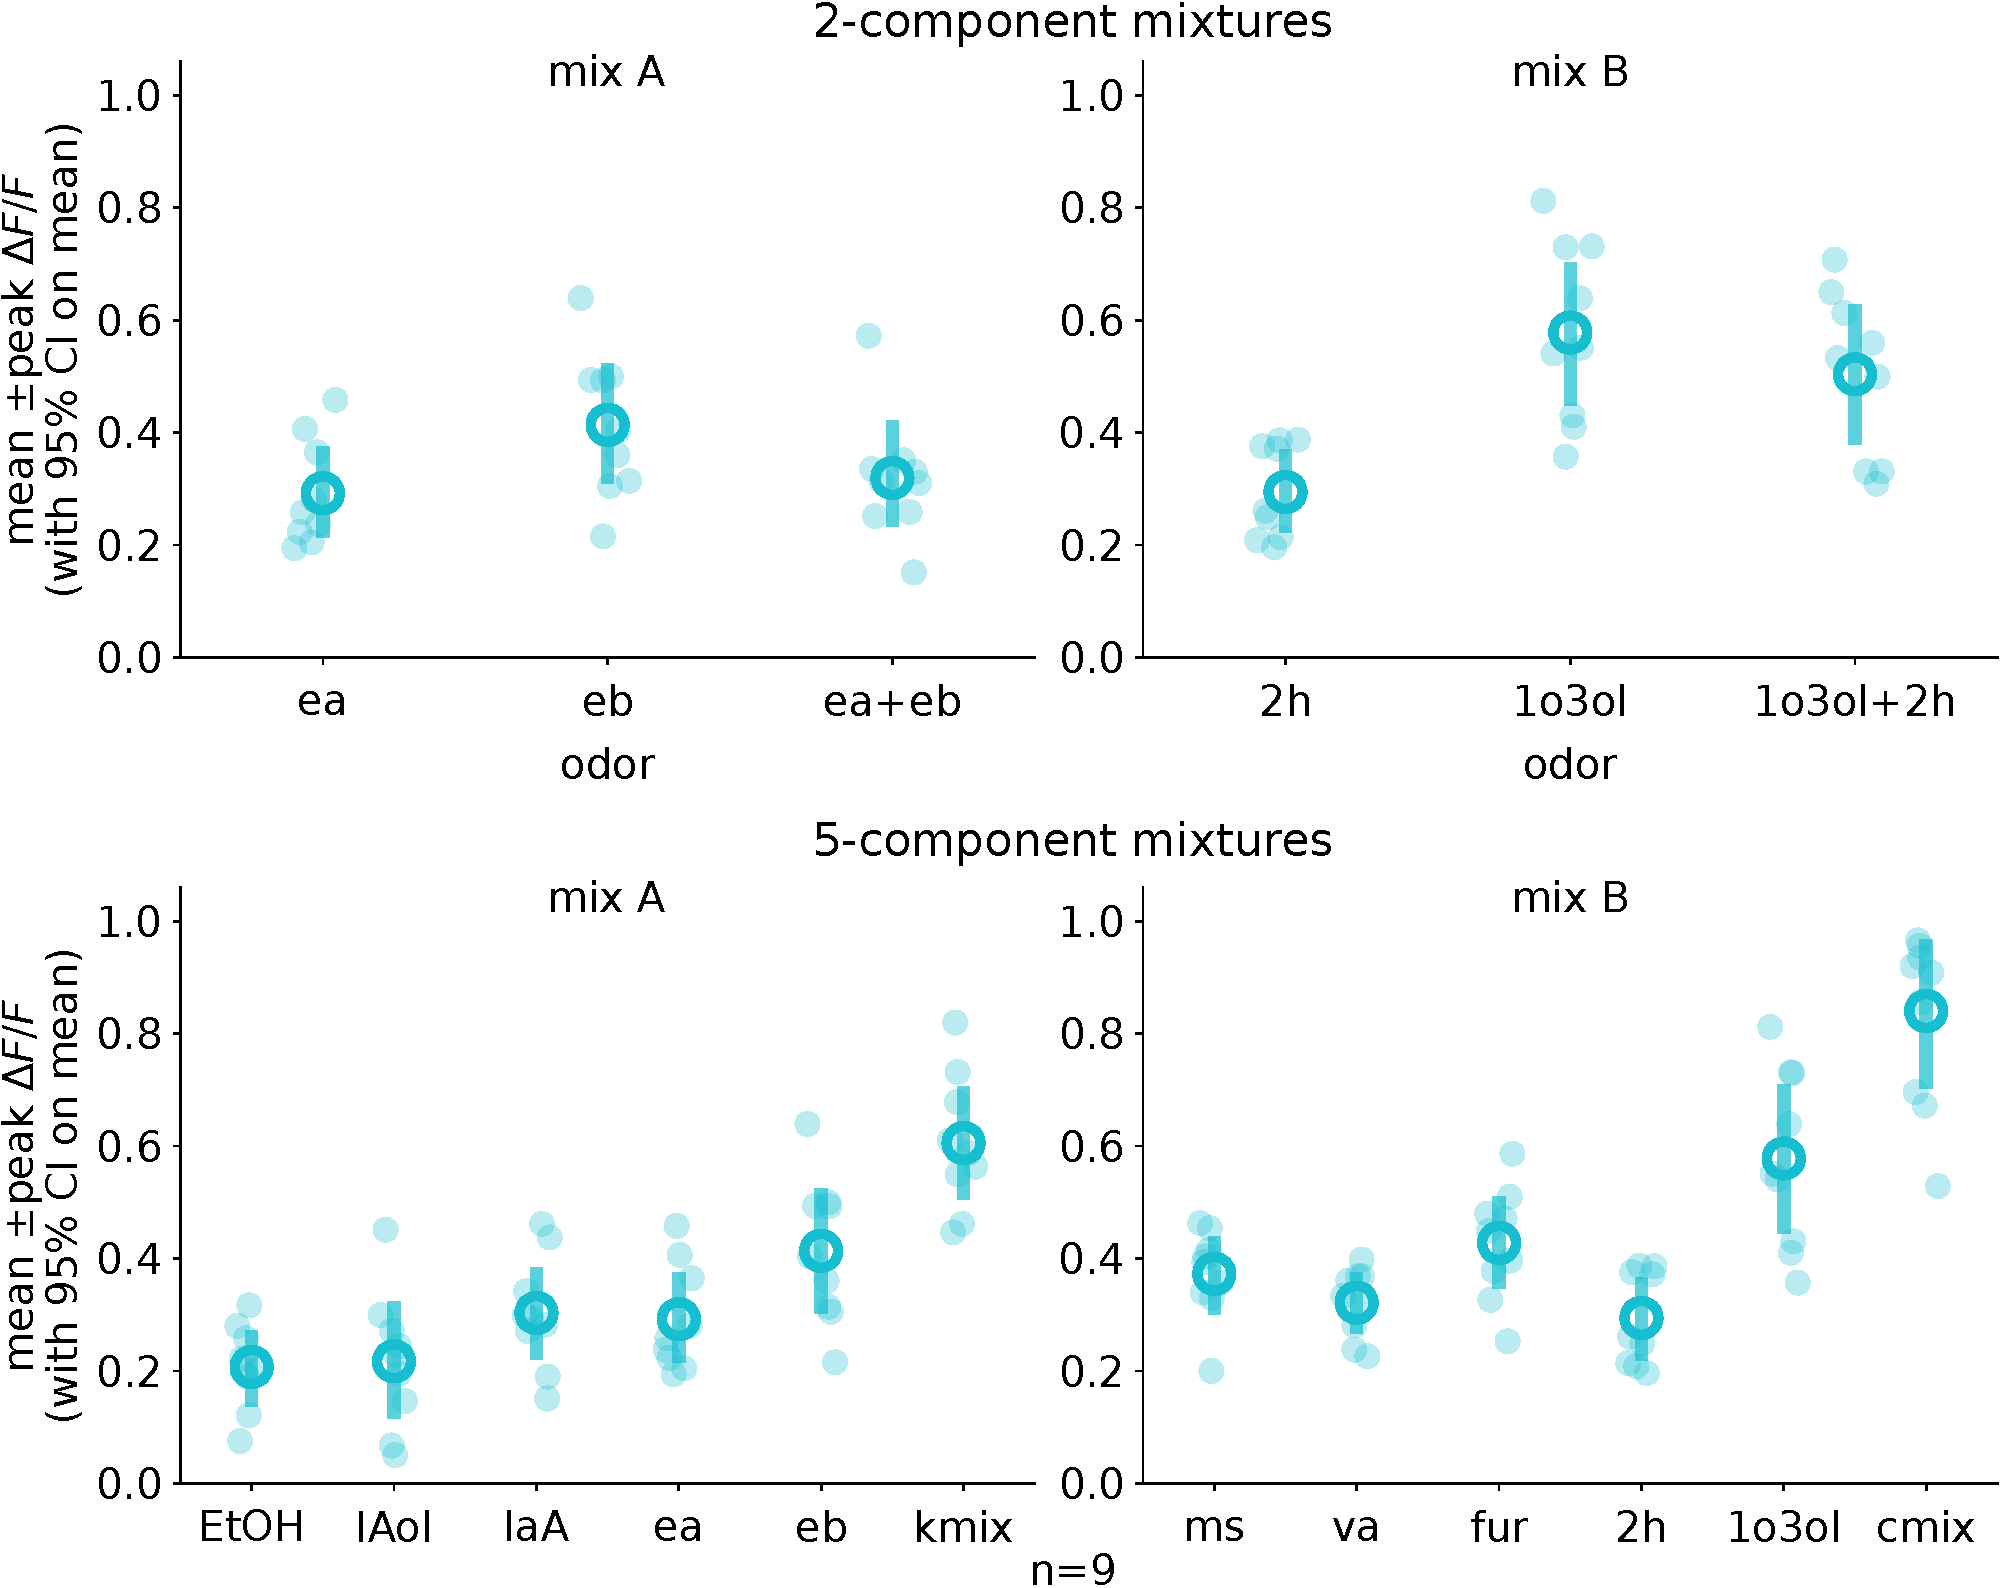
\includegraphics[width=\textwidth]{intensity_orn-only}
\mycaptionof{figure}{Mean ORN response to each odor}{%
Responses were calculated within each fly (per-glomerulus, as described in \cref{fig:orn_mean_responses}), and then averaged across all glomeruli per-fly to produce each of the points shown here. The ea and eb component data is the same across the two- \& five-component plots, as they were only measured once for each fly (in contrast to the KC data, where the binary mixtures are in separate recordings, with separate flies).
}
\label{fig:intensity_orn}
\end{longcapfigure}

\begin{longcapfigure}
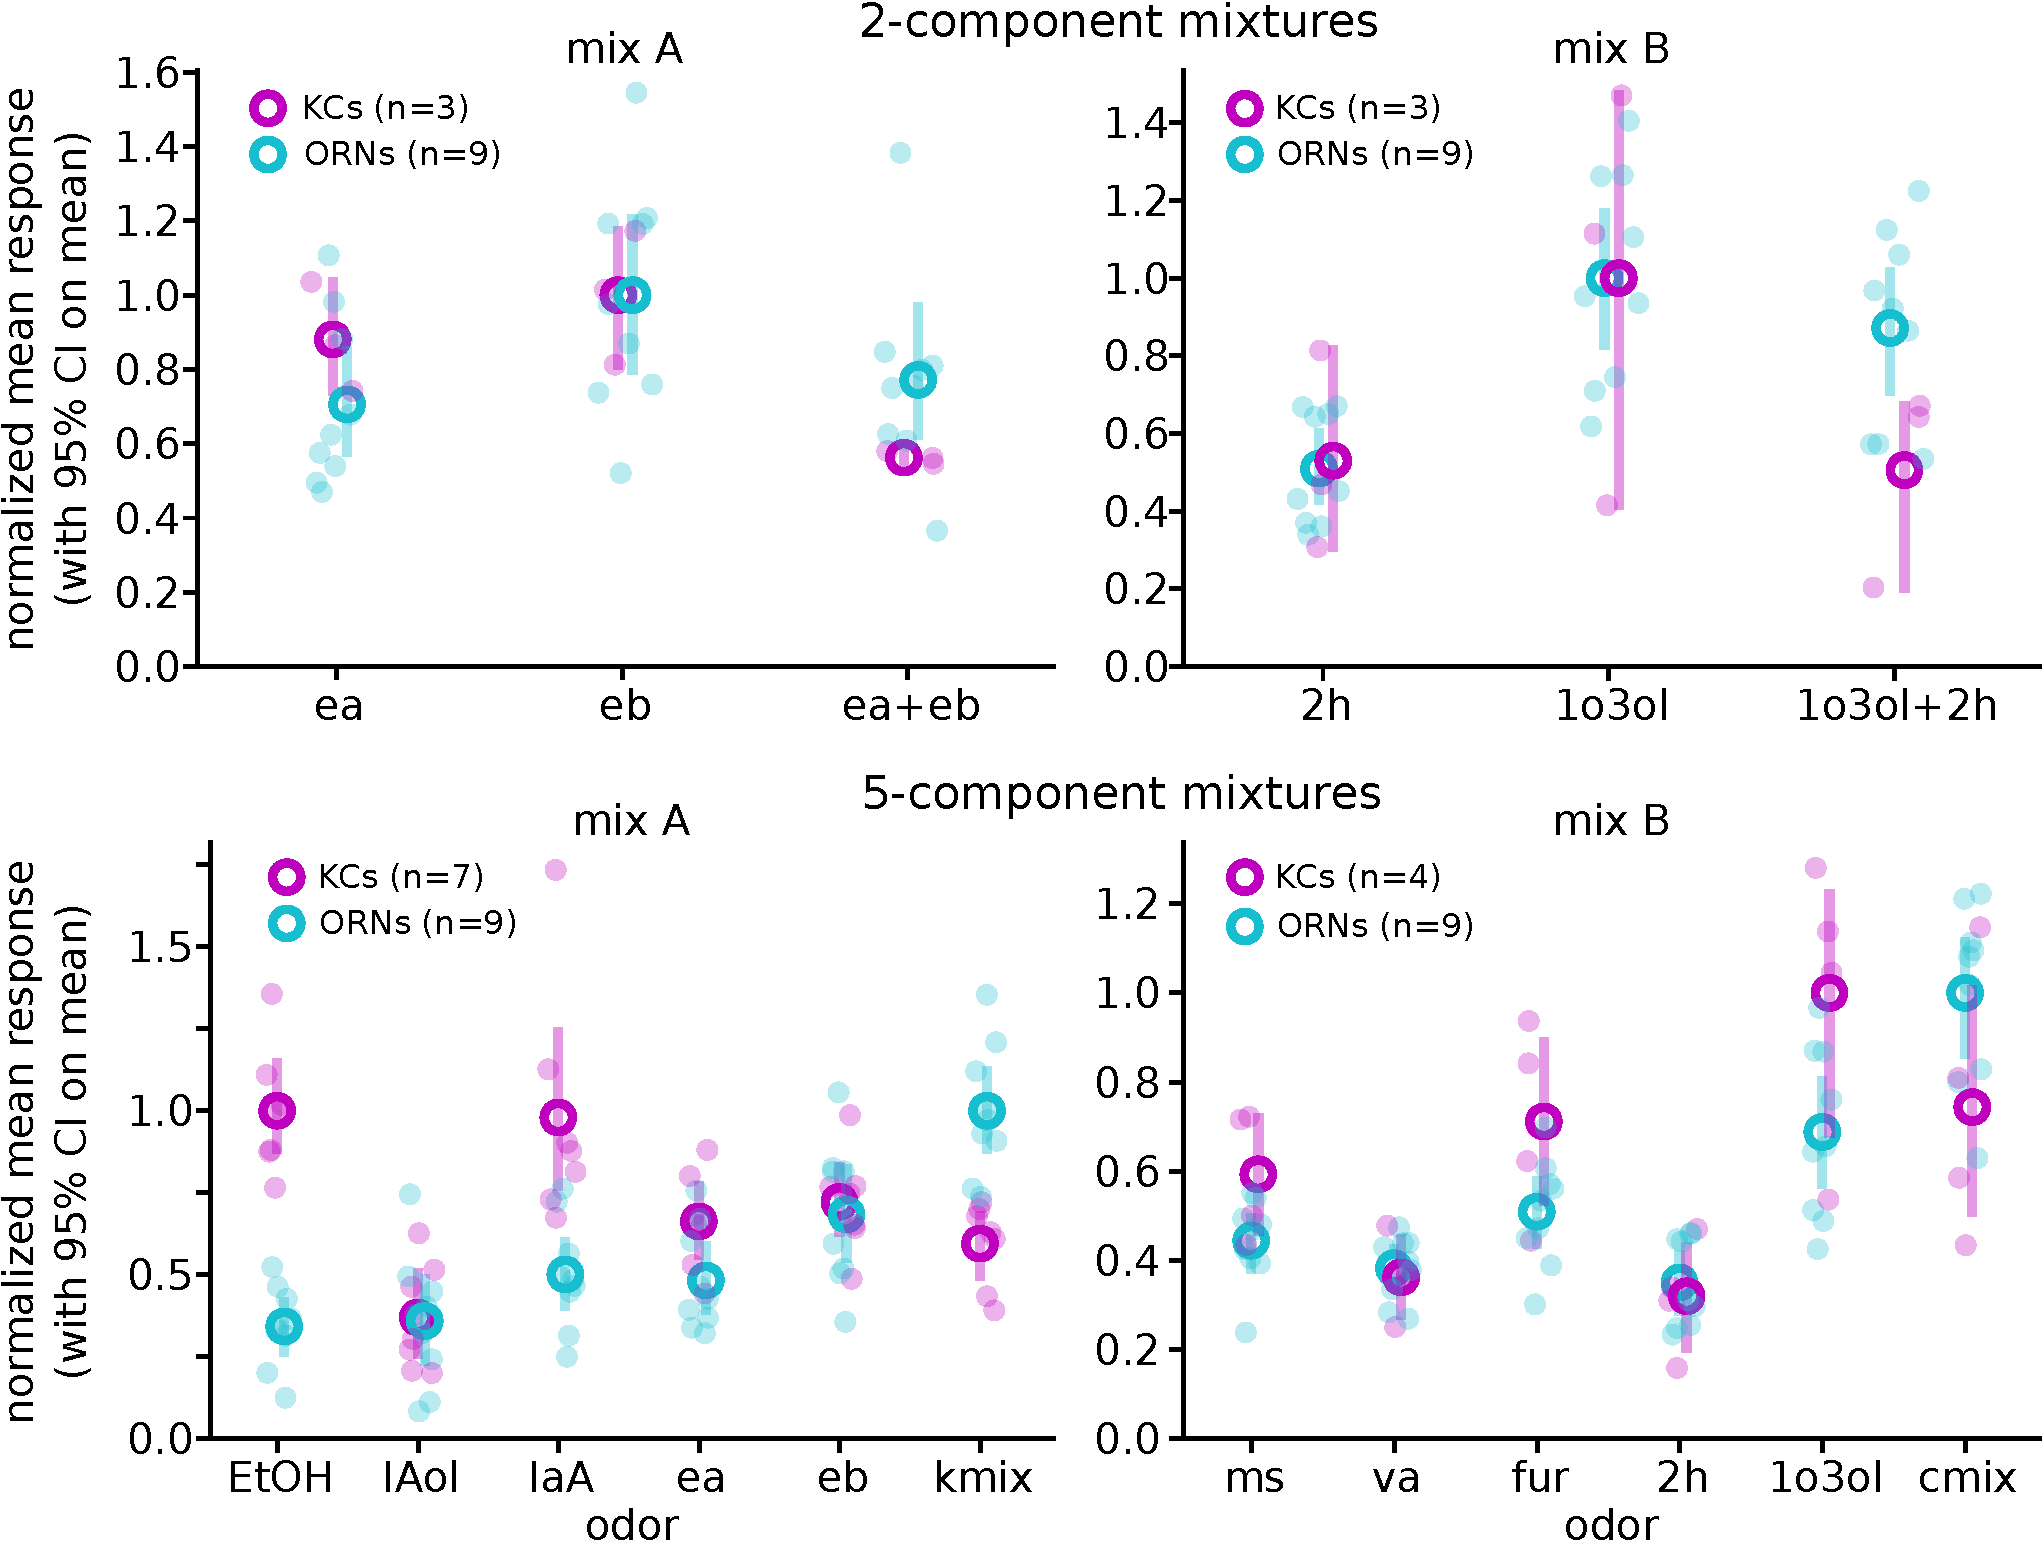
\includegraphics[width=\textwidth]{intensity_orn-vs-kc}
\mycaptionof{figure}{Normalized KC and ORN responses to each odor}{%
ORN data is as shown in \cref{fig:intensity_orn}, but normalized so the odor with the highest mean response has its mean scaled to 1, and all other odors scaled accordingly. The KC normalization works in the same manner, with the purpose being to compare relative activation of odors, and in particular the mix to the most activating component.
}
\label{fig:intensity_orn-vs-kc}
\end{longcapfigure}
% }

\subsection{Model KCs also component-selective, but more mix-responsive than observed}
% TODO model diagram and some example responses?
If the ORN responses do not explain much of our observed KC mixture suppression, can an MB model account for any of these phenomena?
In \autoref{chap:remypaper}, we used an adaptation of Ann Kennedy's biophysically plausible MB model\cite{Kennedy2019} to hint at a contribution of the PN-to-KC connectivity in remapping odor representations to align with natural odor distances.
We adapted that model further in this chapter (see Methods; \nameref{ssec:modeling}), to investigate whether it could recapitulate the tuning and mixture suppression we observed in KCs.
Would there be as many component-selective model KCs as we observed?

Using our ORN data as input, we ran the modified model to get the responses clustered in \Crefwithbackref{fig:clust_hierarch_model}.
We categorized model KC responses into response classes (\crefwithbackref{fig:response-class-means_model_5comp}), as for measured KC responses before.
As in our KC measurements, many model KC responses were selective for individual components (\qtyrange{6.4}{8.7}{\percent}; \crefwithbackref{table:model_vs_kc_resp_types_5comp}), although this was still much less than in our KC measurements (\qtyrange{16.9}{18.6}{\percent}).
However, unlike what we observed in the KCs, the model KC population had many more cells that responded \textit{both} to the mix as well as one or more components (``mix-responsive'') (\cref{table:model_vs_kc_resp_types_5comp}; \crefwithbackref{fig:frac_response_class_model-vs-kc}).
For the binary mixtures $A_2$ \& $B_2$, the model did a much worse job of predicting component-selective cells, and we did not analyze that data in detail.

% Fraction of model and observed KCs in different response classes
\begin{longcaptable}
% TODO TODO TODO also include # responders to each mix, either in this table or elsewhere?
% TODO TODO TODO and/or (only?) report percentages wrt responding fraction?
% (or fraction responding to component in some cases?)
\centering
\begin{tabular}{crcc}
\multirowthead{2}{\thead{Mix}} &
\multirowthead{2}{\thead{Response Type}} &
\multicolumn{2}{c}{\thead{\% of KCs}}\\ \cline{3-4}
  & & \thead{Observed} & \thead{Model}\\
\midrule
\multirow{4}{*}{$A_5$}
% TODO TODO easier way to change textcolor of whole row?
& \textcolor{gray}{non-responding} & \textcolor{gray}{73.1\%} & \textcolor{gray}{83.2\%}\\
% TODO or bold text for these two instead? something else to emphasize (rather than dashlines)? or make text for above and below light gray?
% yea i don't like the dashlines. too busy.
& component-selective & 18.6\% & 6.4\%\\
& mix-responsive & 2.7\% & 7.9\%\\
& \textcolor{gray}{mix-selective} & \textcolor{gray}{0.9\%} & \textcolor{gray}{0.7\%}\\
\hline
\multirow{4}{*}{$B_5$}
& \textcolor{gray}{non-responding} & \textcolor{gray}{76.6\%} & \textcolor{gray}{84.6\%}\\
& component-selective & 16.9\% & 8.7\%\\
& mix-responsive & 3.1\% & 4.5\%\\
& \textcolor{gray}{mix-selective} & \textcolor{gray}{1.7\%} & \textcolor{gray}{0.4\%}\\
\bottomrule
\end{tabular}
\mycaptionof{table}{Model vs KC five-component response type percentages}{}
\label{table:model_vs_kc_resp_types_5comp}
\index{tables}
\end{longcaptable}

% TODO TODO TODO delete much or all of this. esp references to "uniform" model, or claw model improvements relative to it
\iffalse
% TODO delete (/move to supp)
\begin{longcapfigure}
\centering
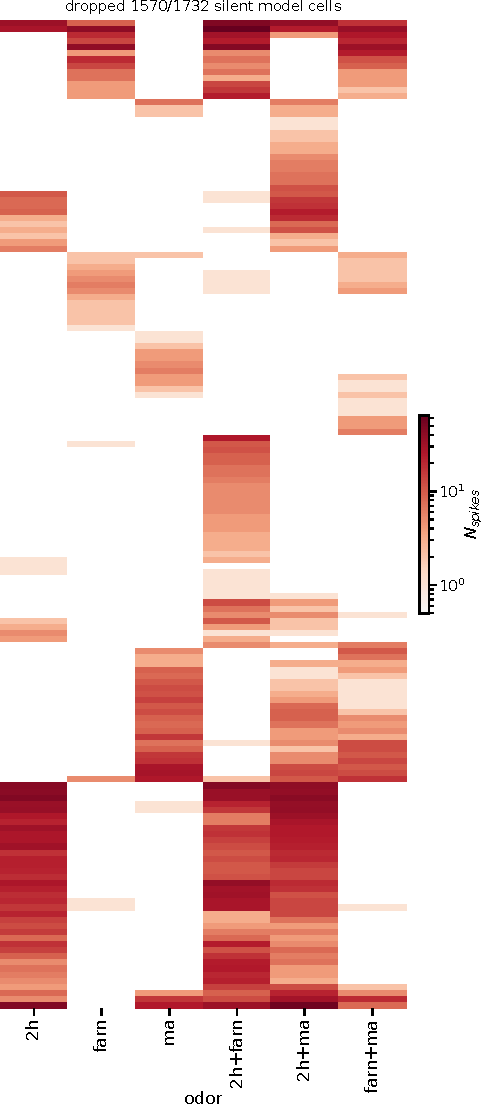
\includegraphics[height=0.85\textheight]{clust_hierarch_diag-binaries_model-claw_trimmed}
\mycaptionof{figure}{Clustered model KC responses to binary mixtures of weak odors}{%
% TODO say anything more here?
Compare with KC responses in \cref{fig:clust_diag-binaries}.
}
\label{fig:clust_hierarch_model_diag-binaries}
\end{longcapfigure}
\textcolor{gray}{
Unlike the mix A \& B cases where we have ORN measurements for all the odors we hoped to model, for the binary mixtures of weak odors we only had ORN measurements for the components\footnotemark[1]{} but not their mixtures.
To still attempt to model the mixture responses of the three weak odors, we took the max across the two mean glomerular response vectors (from measured component data) to generate a synthetic mixture response.
As justification for this approach, we checked the quality of this ORN mixture response approximation for some cases where we did have measurements for both the components and their mix, and the approximation seemed reasonable (data not shown).
After feeding our ORN data (measured components and synthetic mixture) into the two models, we get the responses seen in \crefwithbackref{fig:clust_hierarch_model_diag-binaries}.
For mix A \& B we use our ORN measurements as input, and running the same two models on that data produces the responses in \crefwithbackref{fig:clust_hierarch_model}.
}
% TODO TODO actually expand on this in methods
\footnotetext[1]{The concentrations used between the ORN and KC measurements of these weak components differed slightly. See Methods.}
\fi

% Model hierarchichal clustering
% {
% TODO TODO split out binary model responses and plot separately (and do for ORN data too, like in talk)?
% (probably)
% TODO TODO merge in inkscape, or at least make sure aspect ratio is preserved here
% (that would also help fix current lack of height alignment... or need to handle that separately. bottom edge currently does not align)
\begin{longcapfigure}
  \centering
  % way to add title centered over each subfloat (to label mix A/B here?) (have in input now anyway)
  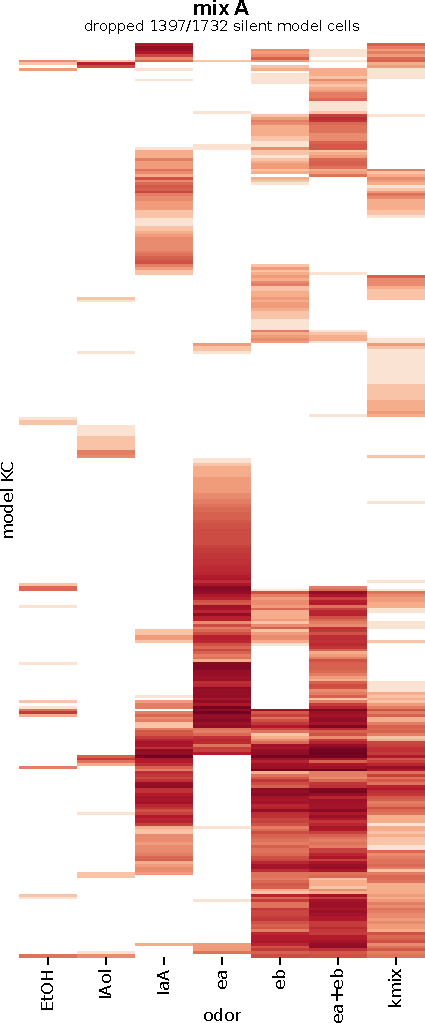
\includegraphics[width=0.43\textwidth,height=0.9\textheight]{clust_hierarch_kiwi_model-claw_trimmed}
  \hfill
  \vrule
  \hfill
  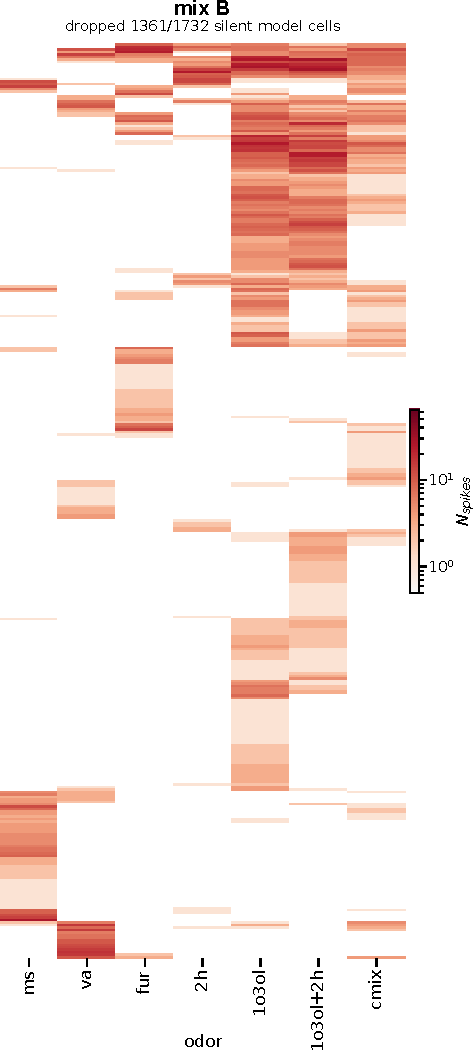
\includegraphics[width=0.50\textwidth,height=0.9\textheight]{clust_hierarch_control_model-claw_trimmed}
\mycaptionof{figure}{Clustered model KC responses to mix A \& B}{%
% TODO talk about spike counts and logistic scale here?
% TODO talk about how it includes both binary and five-comp (or split out)?
Compare with KC responses in \cref{fig:clust_hierarch_binary,fig:clust_hierarch_5comp}.
}
\label{fig:clust_hierarch_model}
\end{longcapfigure}
% }

% Model response classes
% {
\begin{longcapfigure}
\centering
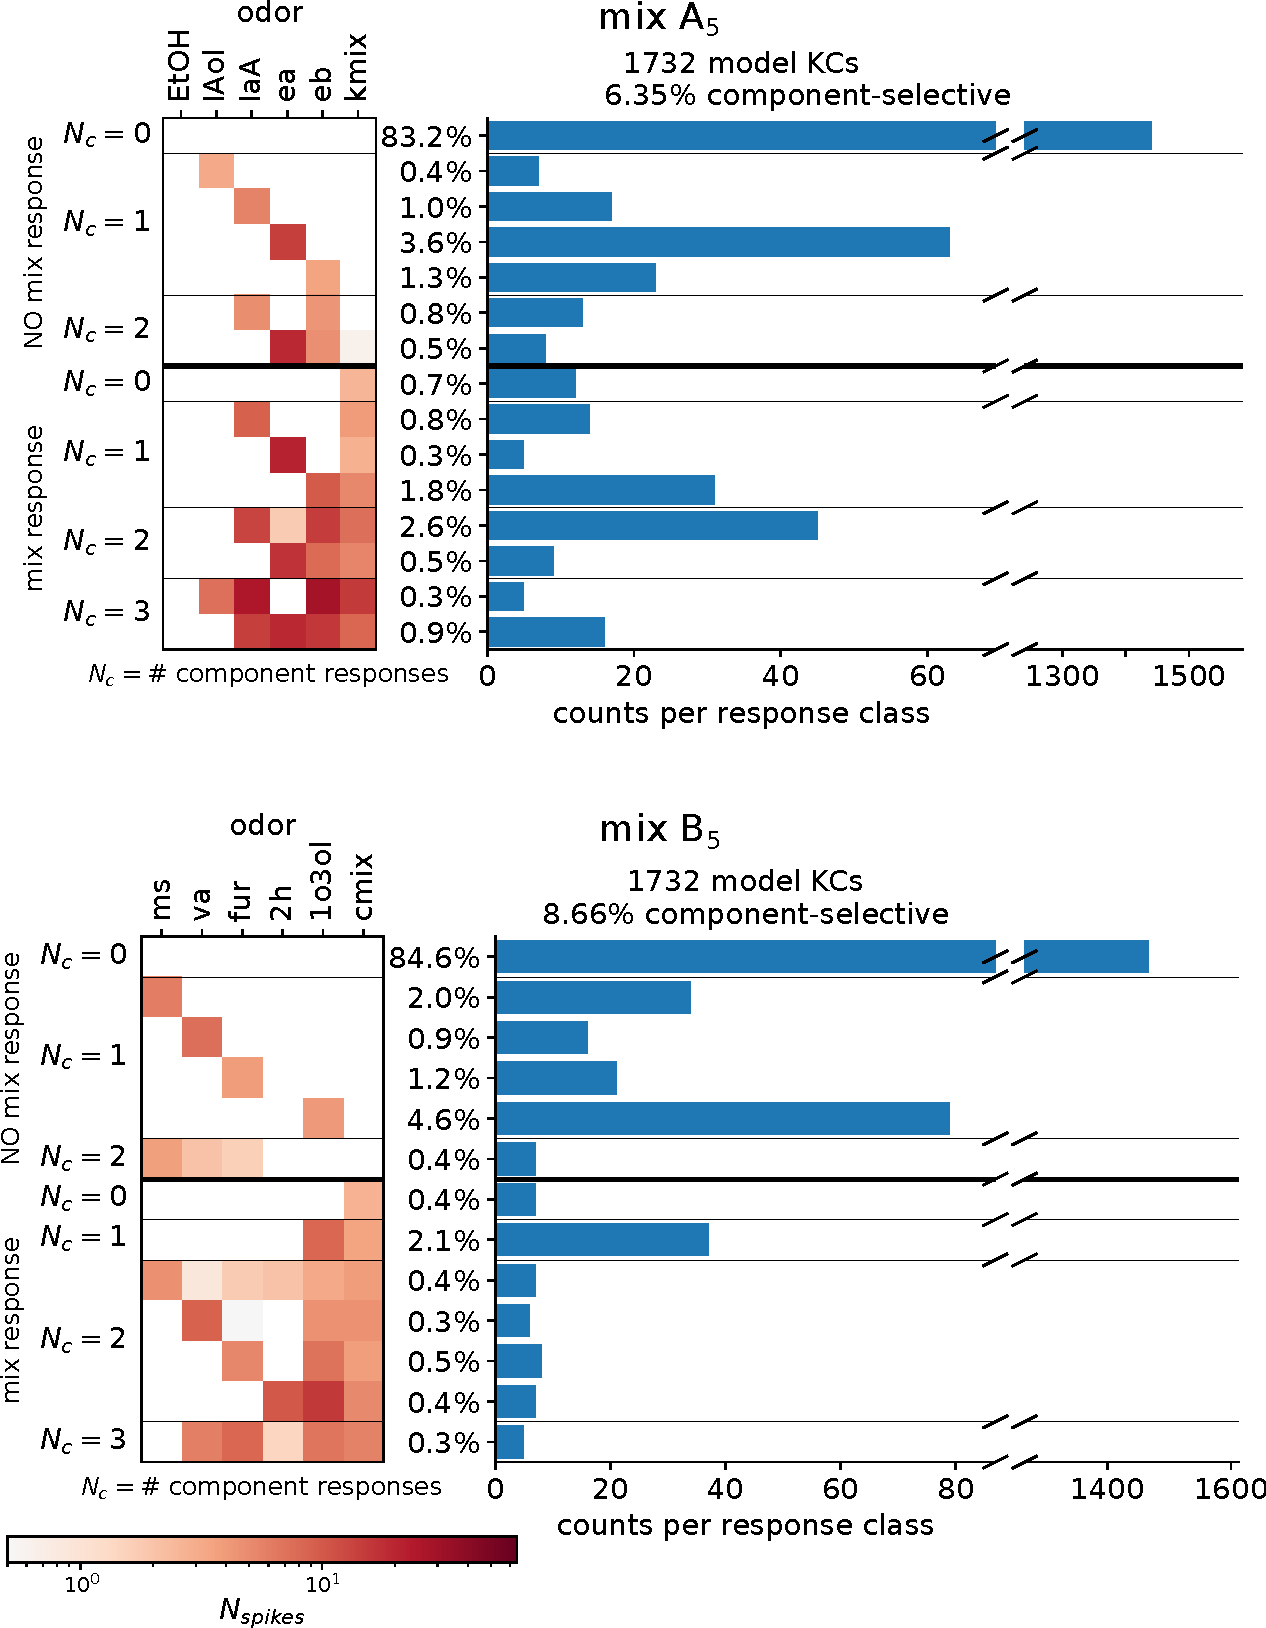
\includegraphics[width=\textwidth]{response_class_means_and_counts_kiwi-control_claw-only}
\mycaptionof{figure}{Model five-component mix A response class means and counts}{%
% TODO move to methods (+ delete everywhere)
%Classes containing less than 0.25\% of ROIs have been excluded, so percentages may not sum to 100.
% TODO delete text (already in table) refer to table!
%Mix-responsive fractions are 7.91\% for mix A and 4.45\% for mix B.\\
Compare to KC tuning in \cref{fig:response-class-means_kc_5comp}.
}
\label{fig:response-class-means_model_5comp}
\end{longcapfigure}
% }

% Response class summary: model vs KCs
\begin{longcapfigure}
\centering
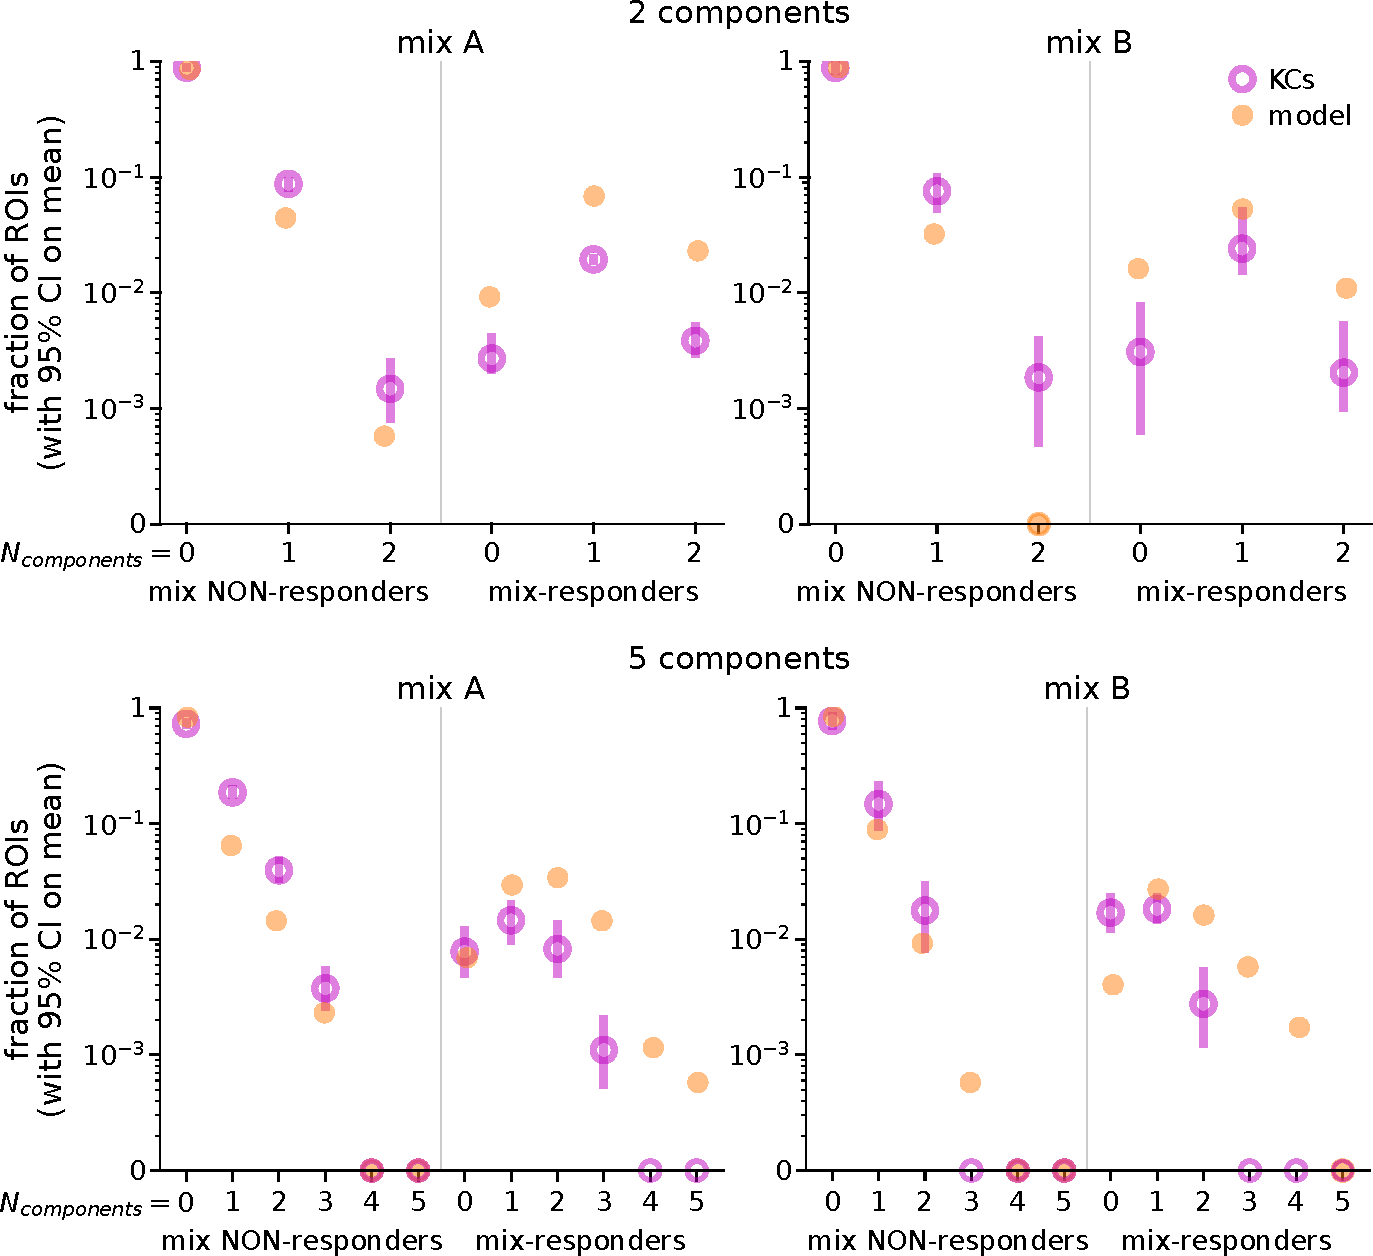
\includegraphics[width=\textwidth]{frac_response_class_model-vs-kc}
% TODO better name in this caption than "response class summary"?
\mycaptionof{figure}{KC \& model response class summary}{%
% TODO delete (that other fig may not be presented now, at least not maybe till supplement)
%Similar to \cref{fig:frac_response_class_kc-orn}, but now on a log scale. KC data is same for both.
Response classes grouped by whether they are mix-responsive and their number of component responses, ignoring which component had the maximal response.
}
\label{fig:frac_response_class_model-vs-kc}
\end{longcapfigure}

\iffalse
\subsection{Comparing model and measured KC response intensity}
% TODO TODO keep? move to supplement?
%
% Model vs KC intensity in weak binaries
\begin{longcapfigure}
\centering
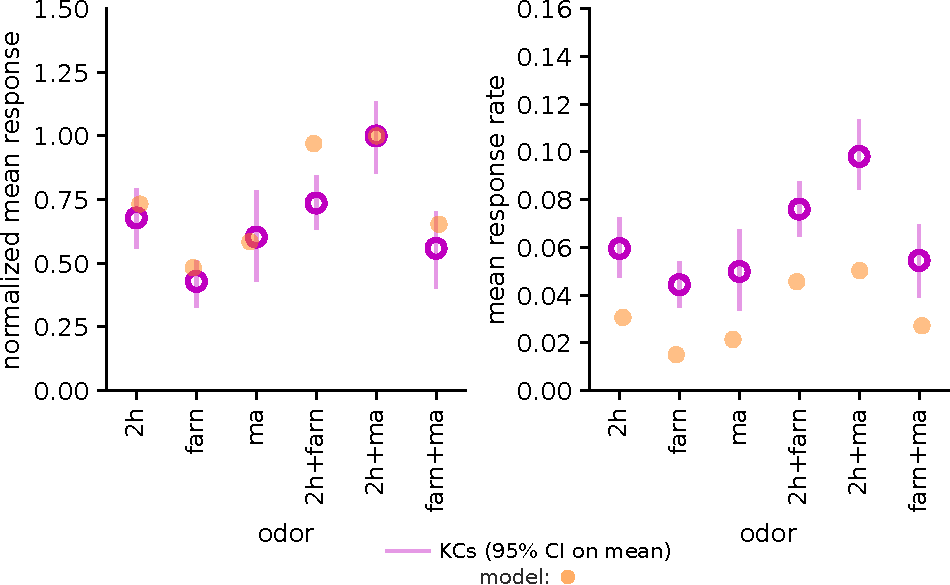
\includegraphics[width=\textwidth]{intensity_diag-binaries_model-vs-kcs}
\mycaptionof{figure}{KC and model average responses to binary mixtures of weakly-activating odors}{%
% TODO say more?
% TODO also refer to either methods or first KC-only figure for description of top statistics
KC response calling (for right panel), is as described in \cref{fig:clust_diag-binaries}.
}
\label{fig:intensity_diag-binaries_model-vs-kcs}
\end{longcapfigure}
\fi

% nvm, farn also activates VM5v reasonably (just a bit less than DC3) and that is (not nothing) but towards the lower side of # synapses per glomerulus
%It is actually somewhat surprising that the claw model does a better job of predicting farn response strength, with the decrease in its relative (across odor) strength compared to in the uniform model, because the glomeruli this odor activates are DC3 (
% TODO (move this comment to relevant script) why does uniform overpredict farn, if DC3 one of the glomeruli with the higher #'s synapses into the KCs??? are all those inputs to a select population of KCs?

% TODO (move comment to relevant script) maybe i should also try a plot like this, that doesn't group across components w/ maximal response (and fills x axis to union of all inputs, as this one currently does) (though prob not for thesis)

\subsection{Model KCs capture some mixture suppression, but less than observed}

% TODO maybe i should be doing a non-normalized version of intensity plot (w/ avg logistic scaled vs avg \KCRespStat), if that scaling really brings things in line (and maybe parameters should be changed to better improve that match, if not good already? optimizing wasserstein distance also have effect of improving that, or not really?)

% TODO TODO delete (/ move to supplement?)
\iffalse
% Mix suppression dists and means for weak binaries (model vs KCs)
% {
\begin{longcapfigure}
\centering
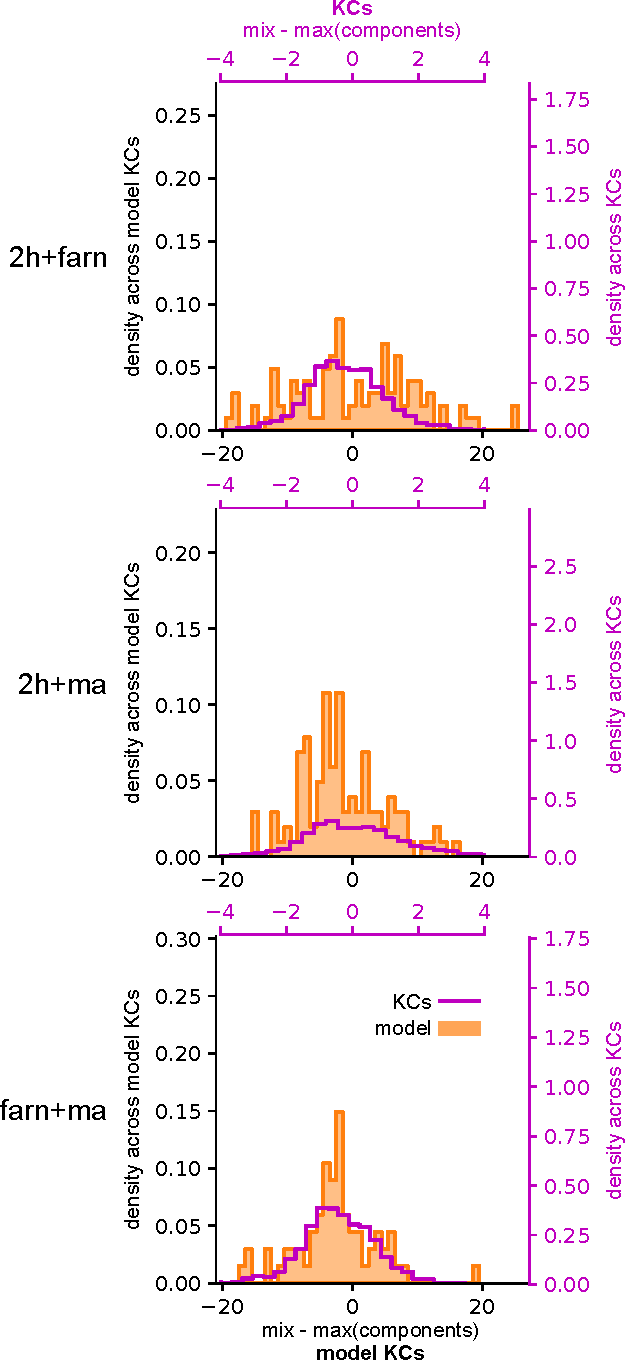
\includegraphics[height=0.85\textheight]{mixsupp_dists_diag-binaries_model-vs-kcs_no-logistic}
% TODO TODO be consistent about "weakly-activating" vs "weakly activating"
% TODO TODO also be consistent about "logistic-scaled" vs "logistic scaled"
\mycaptionof{figure}{Distributions of KC and model mixture suppression to binary mixtures of weakly-activating odors}{%
% TODO \NSpikes here?
Model KC mixture suppression computed on raw spike counts.\\
KC distributions replotted from \cref{fig:mixsupp_dists_diag-binaries_kc-only}.
% TODO delete?
Each row is one of the three mixtures of weakly-activating odors, with the odor pair in the label on the left.
}
\label{fig:mixsupp_dists_diag-binaries}
\end{longcapfigure}
\begin{longcapfigure}
\centering
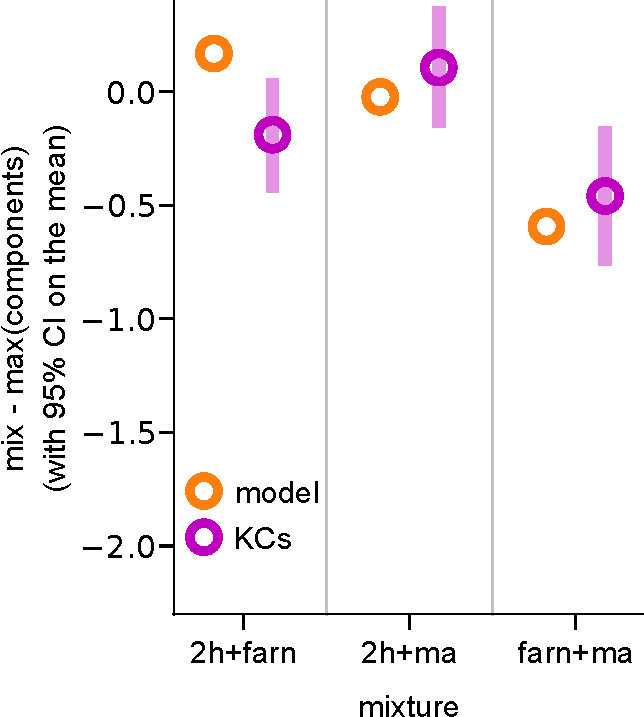
\includegraphics[height=3in]{mixsupp-avg_model-logistic-scaled_vs_kc-model_diag-binaries}
\mycaptionof{figure}{Mean mixture suppression across models and KCs for weak binary mixtures}{%
For the model data, mixture suppression was computed on logistic scaled \NSpikes.
For KCs, the computation is as before.
}
\label{fig:mixsupp-avg_model-logistic-scaled_vs_kc-model_diag-binaries}
\end{longcapfigure}
% }
\fi

% Mix suppression dists and means for mix A/B (model vs KCs)
% {
\begin{longcapfigure}
\centering
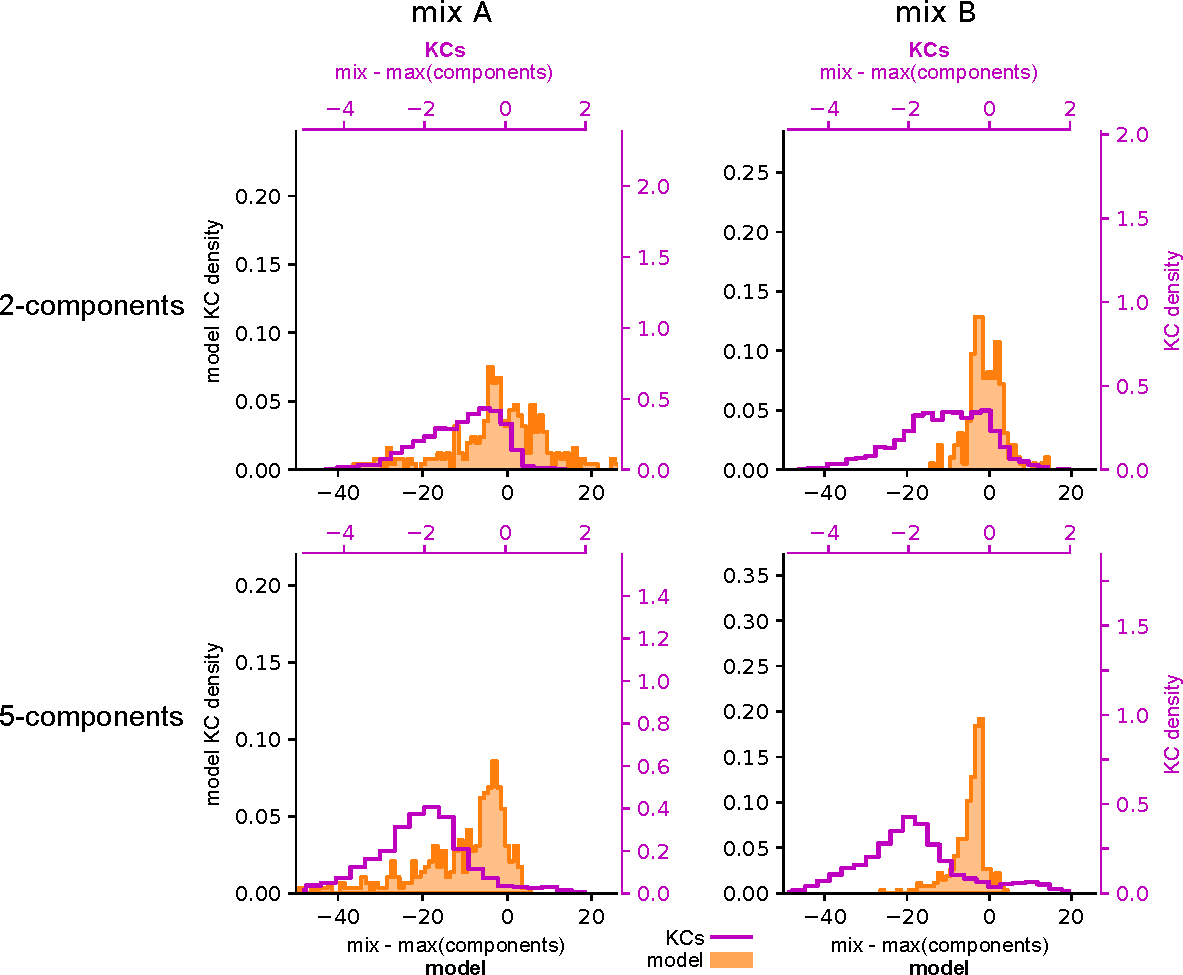
\includegraphics[width=\textwidth]{mixsupp_dists_kiwi-control_model-vs-kcs_no-logistic}
% TODO change caption label here?
\mycaptionof{figure}{Distributions of KC and model mixture suppression}{%
% TODO NSpikes instead?
Model mixture suppression computed on raw spike counts (\NSpikes).\\
KC distributions replotted from \cref{fig:mixsupp_dists_kc-orn}.\\~\\
Plots with each dataset (either the KCs or the model KCs) were made so that a fixed horizontal scale contained most of the data (across mixtures), and then the plots were aligned to place 0 in the same horizontal position. Note how all panels share one magenta and one black horizontal scale.\\~\\
All five-component distributions show mixture suppression (via the left-shift).
Unlike the KCs, the model has distributions roughly centered around 0 for both of the binary mixtures.
}
\label{fig:mixsupp_dists_kiwi-control_model-vs-kcs}
\end{longcapfigure}

\begin{longcapfigure}
\centering
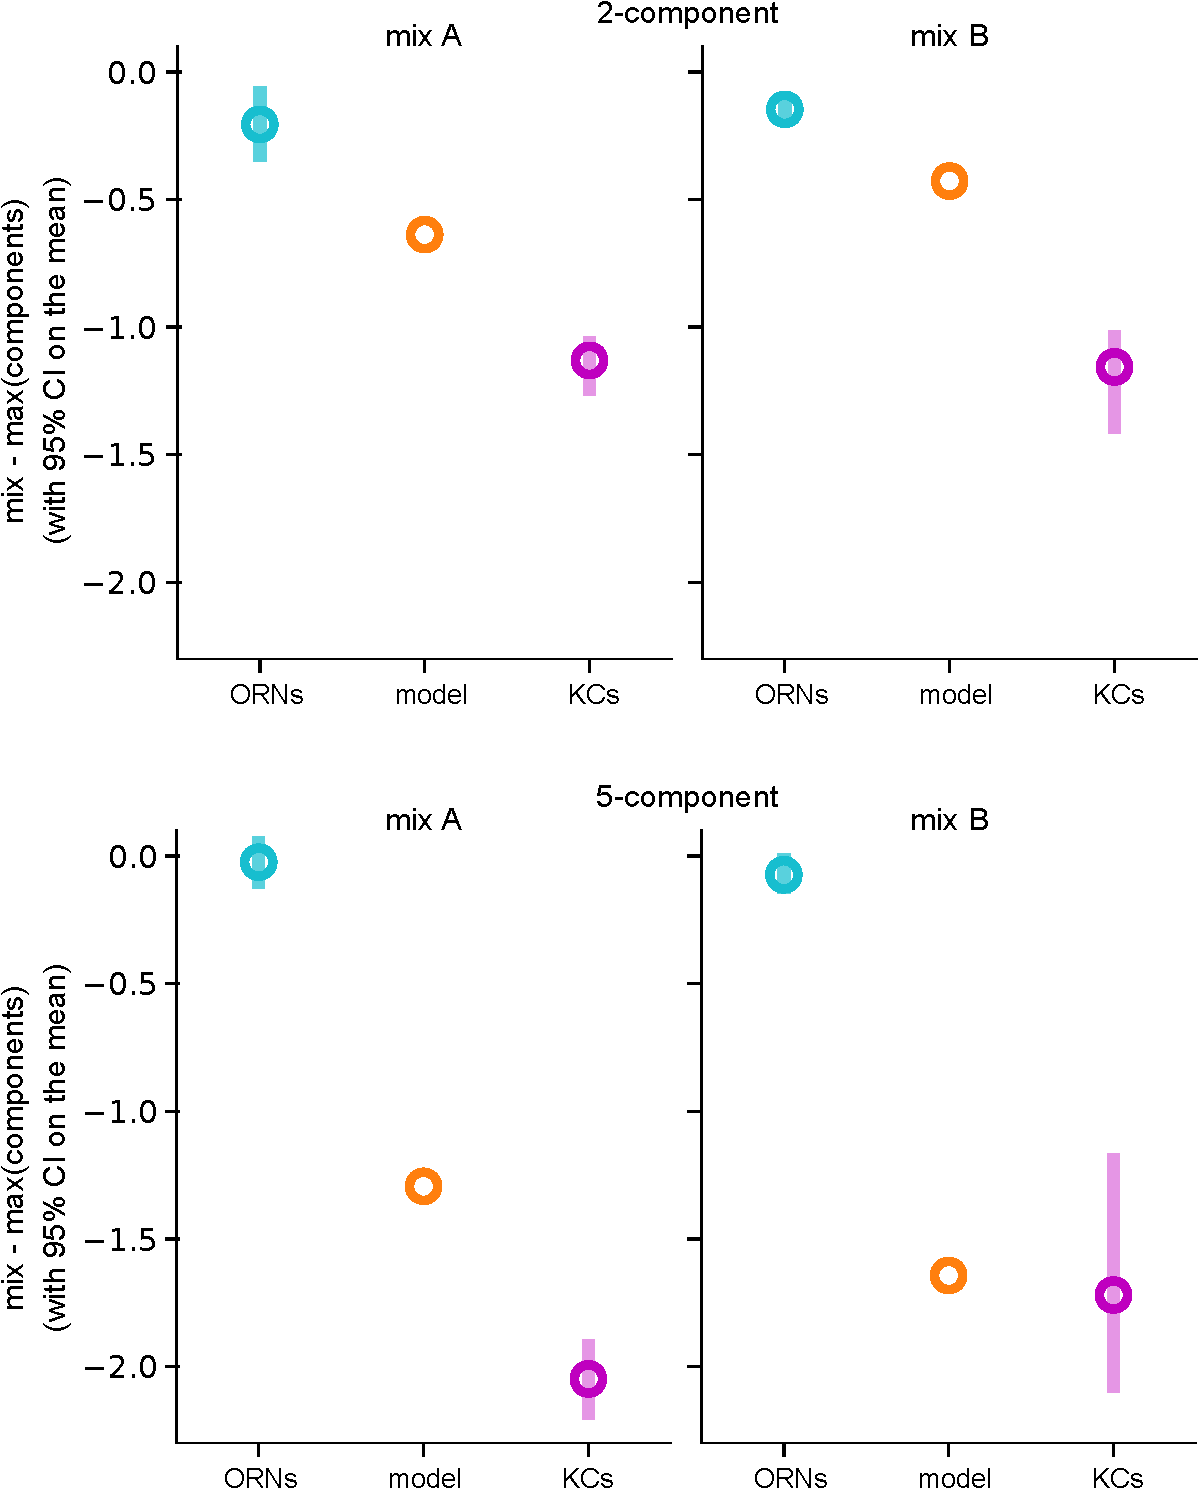
\includegraphics[height=4in]{mixsupp-avg_model-logistic-scaled_vs_kc-orn}
\mycaptionof{figure}{Mean mixture suppression across ORNs, model, and KCs}{%
% TODO get this link to work, without showing meaningless page number (or what even is it?)?
%For the model data, mixture suppression is computed on logistic-scaled \NSpikes{ }(see Methods \ref{sssec:scaling_spike_counts}).
For the model data, mixture suppression is computed on logistic-scaled \NSpikes{ }(see Methods).
For ORNs \& KCs, the computations are as before.
}
\label{fig:mixsupp-avg_model-logistic-scaled_vs_kc-orn}
\end{longcapfigure}
% }

% TODO add note about how different ORN response amplitude distribution might affect things? still would expect to pretty much be 0... although it's ~-0.2 in binary (kiwi case only, and it does appear real)

Given that the model has a reasonable proportion of component-selective cells (at least, in the five-component mixture context), we expected the model to show mixture suppression to at least the five-component mixtures.
%Since the model also exhibits more mix-responsive (but \textit{not} mix-selective) cells to these mixtures, we also expected that the extent of the suppression may not match our KC measurements.
We started by computing model mixture suppression using the raw spike counts (\NSpikes) the model emits to each odor, and qualitatively aligning those distributions to the KC mixture suppression distributions we computed earlier (\crefwithbackref{fig:mixsupp_dists_kiwi-control_model-vs-kcs}), and we did see many model KCs exhibiting suppression to the five-component mixtures, though perhaps not to the same extent as the real KCs.
For both binary mixtures, the model distributions showed much less mixture suppression than the real KCs.

% TODO fix subsubsection link?
Since the model spike counts have a rather different range than our KC measurements, I scaled the model outputs into a range similar to the KC data, to compute more directly-comparable mixture suppression values (see Methods). %\cref{sssec:scaling_spike_counts}).
For mix A \& B (both the two- \& five-component versions), the KCs had higher average mixture suppression than the ORNs, and the model sat at intermediate values (\crefwithbackref{fig:mixsupp-avg_model-logistic-scaled_vs_kc-orn}).
For the five-component mix B, it sat well within the error bars on the KC mean.
The model again showed much less mixture suppression than KCs to the binary mixtures, consistent with the qualitative impression of the prior distributions (\cref{fig:mixsupp_dists_kiwi-control_model-vs-kcs}).
As with the real KCs, the model exhibited much more suppression to both five-component mixtures than to either binary mixture.
% TODO delete?
%The poor predictions here are not surprising because other more basic features of these binary mixture responses were also poorly predicted above.

% TODO move to discussion / delete
%However, the changes made to get the model to show meaningful mixture suppression in the 5-component case (moving from the uniform to the claw variant) may also suggest avenues to push further, in order to capture the observed 2-component mixture suppression, and hopefully better capture the KC mixture responses more generally.

% TODO TODO delete (/save for discussion)?
% TODO where was i going with this?
%We have long known that a majority of the responses produced by this dynamic model are single spikes shortly after odor onset, which seemed to be more a quirk of the model behavior, rather than something that resembled a feature of our KC measurements.
%In our KC measurements, there is not typically such a small fraction of responses occupying the higher end of the response dynamic range, which is a consequence of this model behavior.
% TODO TODO now talk about how it makes sense to add delay for APL to act

% TODO want \processdelayedfloats here? or maybe after discussion but before methods
% (that's where i put it now, up from right before references where it was before)?

\section{Discussion}
\subsection{Strong ORN responses are broad with ``hypoadditive'' mix responses}
We observed that most glomeruli respond broadly and those that respond to a component almost always respond to the mix.
Glomeruli that respond to a mix also tend to respond to at least one component with a similar magnitude.
% why reference to fig:mixsupp_dists_kc-orn not defined here? oh, seems it was a space after ',' causing the issue
For glomeruli with strong mean responses ($\geq\!0.8\,\DeltaFOverF$ to any odor), we saw no clear examples where the mean is much more (or less) to a mix than to its most activating component (\cref{fig:orn_mean_responses}).
Some early work in the mitral/tufted (M/T) cells of the (mouse and rat) olfactory bulb (OB) has also described this as a common type of tuning (termed ``hypoadditive'', borrowed from psychophysics) in these cells analogous to \textit{Drosophila} PNs\cite{Giraudet2002, DuchampViret2003, Davison2007}.

Among these glomeruli with strong mean responses to some components, two glomeruli (VC2 \& VC3) may have shown a weaker binary mix B response than to some of its components.
This effect may be outweighed by excitation from the remaining components in the five-component case.
Another large class of possible exceptions are glomeruli with weak responses to all odors we presented, where many of these weak component responses seemed to be diminished when the mixture is presented (e.g. DC2 for mix B, or DL2d / VA3 for mix A).
% TODO delete? rephrase above (/replace w/ this)?
% (e.g. DC2 for either variant of mix B, or DL2d / VA3 for mix A).
Our mean ORN responses may only be exhibiting this ``hypoadditive'' (rather than ``mix suppression'') behavior when the responses to one component alone are already saturating, and we would need to do further ORN experiments to clarify whether the same glomeruli that seem ``hypoadditive'' in their strong responses here exhibit the same behavior at lower concentrations of the same components and mixtures.

Since we measured signal in ORN axon terminals at the glomeruli, it is possible that some of the behavior we see is a result of lateral excitation or inhibition.
One way to rule out most lateral effects would be to record upstream parts of the ORN (e.g. with sensilla spike recordings), similar to the comparisons between glomerular and cell body recordings in \textcite{Zak2020}.
With the uncertainty of whether hypoadditivity is only dominant in saturating regimes and the possible effects of lateral interactions at the ORN axon terminals in the AL, we cannot conclusively say that our ORN results are inconsistent with a growing body of literature that argues for the importance of inhibitory interactions between component odors at the receptor level, via competitive binding or antagonism\cite{CompetitiveBinding, MurthyAntagonism, Zak2020}.
However, suppression was not the dominant effect we saw in our ORN measurements, at least among the glomeruli with strong mean responses to at least one odor.
% TODO delete? or do they actually not see much at lower concentrations?
%The odor concentrations where this receptor-level inhibition is observed are often much higher than in this study\cite{Zak2020}, where we used more naturalistic (lower) concentrations\cite{ConcentrationReview}.
%It is not yet clear if these receptor-level interactions play as large a role at lower concentrations.

Inconsistent definitions of mixture suppression may also contribute to possible discrepancies between our observations and prior studies.
Some of the analyses claiming mixture suppression compare mixture responses to the linear sum of the component responses, rather than to the most-activating component.
This would tend to overstate the extent of any suppression, in cases where any component alone can bring a response near saturation.
Some work that includes both calculations shows much smaller effects when comparing the mixture response to the component-maximum, rather than the linear sum of component responses\cite{Zak2020}.

% TODO reword?
Finally, our study may not have examined sufficient numbers of odorant interactions to reveal examples of mixture antagonism at the odorant receptor.
Extending our approach to additional mixtures with greater chemical diversity and which target a broader population of receptors may reveal examples of mixture antagonism at the level of the receptor.
% not even hints of this to talk about. delete.
% in ORN distributions, there might be a hint of slightly *more* binary mix suppression (but within errorbars on mean plot)
% in KC data, the binary data seems equiv across two panels and what i was originally talking about is that mix A5 is trending
% towards more mixsupp than B5, but B5 only has 4 flies and is much noisier. errorbars do overlap, but not by much.
% (and regardless, this section is talking about ORNs not KCs, so irrelevant)
%It would be interesting if other naturalistic mixtures, or particularly food-related odors (as our ``mix A''), tend to exhibit less inhibitory receptor interactions than arbitrary combinations of chemicals.

% TODO TODO to what extent should i move this stuff up to intro?
\subsection{Existing literature does not clearly establish mixture suppression in KCs/PCx}
\subsubsection{KC literature}
Besides the work in this chapter, \textcite{Endo2020} is the only other study that attempts to image complete KC populations to mixtures.
Although they do not explicitly analyze mixture suppression, they do cluster their cells and report the fractions in these clusters with different tuning.
Their clustering seems to indicate that KCs exhibit less mixture suppression than PNs, if anything.
The three largest clusters they observe are either mix-selective, which is hardly something we saw at all in our binary mixtures; or segmenting in the same manner as the cells from \textcite{LocustKCMixSpiking}, where the cells respond to one component as well as the mixtures that contain it.
Given the limited nature of the stimuli in this study, and the lack of clarity of response diversity within their clusters, it is hard to draw conclusions about mixture suppression.
Although they only sample \textasciitilde6\% of the total KC population, \textcite{Campbell2013} provide another example where KC responses to the mixture seem to largely lie in-between those of the components, at least for their binary mixtures at high concentrations.

\textcite{Lin2014} is interesting because they explicitly show that the APL is important for reducing the response to their binary mixtures, since they see an increased response to their binary mixtures (but \textit{not} to a separate monomolecular odor) when the APL synaptic output is blocked by temperature-sensitive shibire (\ShibireTsShort).
Unfortunately they do not directly compare the mixture response to the responses of the constituent components in the same experiments and analysis, so it is hard to say to what extent they are seeing binary mixture suppression as we did, or to compare the magnitude.

Finally, \textcite{LocustKCMixSpiking} measure KC responses to the most complicated mixtures, with up to eight components.
The main limitation of their study is that they only sample at most a few hundred KCs per locust, out of a total population of \textasciitilde\num{50000}, and they acknowledge that their experimental methods may have biased them towards finding the ``segmenting'' KCs they discuss as the dominant type of tuning they observe.
In the text, they also mention they found some fraction of KCs selective to certain mixtures they presented (including those with at least three components), but they unfortunately do not describe what fraction of cells they found with each type of tuning.
With their limited sampling, such a breakdown of tuning would also probably be of limited value.
Despite their possible sampling bias, we hardly saw any KCs that responded to the component as well as the mixture, and it is certainly not a dominant type of tuning we observed.

\subsubsection{Mammalian PCx literature}
Although there is existing evidence for mixture suppression in the PCx neurons analogous to KCs\cite{PiriformMixSupp}, they only used one simple binary mixture, they did not quantify fractions of the population exhibiting this behavior, and for their qualitative analysis they defined cells as exhibiting mixture suppression if their mix response was less than the \textit{sum} of the component responses (which would overestimate the fraction, compared to our calculation).
\textcite{Rokni2020} also show that PCx neurons are again biased towards mixture suppression, now with up to four components, but with spike recordings that only sample fewer than 100 neurons, and using the same calculation with respect to the sum.
\textcite{Zak2024} do find feedback from PCx neurons, that increases with both concentration and mixture complexity, but they only measure this PCx feedback signal via its boutons in the OB.

\subsection{KCs predominantly respond selectively to single components}
%While 
%The existing KC literature scarcely sees mixture suppression in at all.
%Some PCx and only poorly sampling and characterizing it in the PCx, I will describe our KC results, and provide one reason to be skeptical of them.

We observe that most KCs respond selectively to single component odors, and \textit{not} to mixtures that contain them.
The fact that this is the dominant type of response implies that there is meaningful suppression away of the mixture response, and is thus equivalent to saying that we saw strong mixture suppression for all our mixtures.
This suppression away of the mixture response was stronger to the five-component mixtures, but was also the most common behavior in the binary case.
%Only a small number of studies have recorded KC mixture responses, and most of their mixtures have been binary mixtures of odors at high concentrations\cite{Campbell2013,Lin2014,Endo2020}, but it nonetheless difficult to reconcile our measurements with theirs.
It is unclear why prior KC experiments did not see clear signs of mixture suppression, or whether it can be explained away by peculiarities of their high concentrations, their particular choice of odors, or their typically worse KC sampling.
%On balance, I think this is unlikely.

Despite how many mix-responsive glomeruli we observed (\cref{fig:frac_response_class_kc-orn}), it is quite surprising that we saw far fewer mix-responsive KCs.
For all mixtures, the total KC mix-responsive population was between \qtyrange{2.6}{3.6}{\percent}, which was lower than the highest fraction of component-selective cells in each mixture's components (\cref{table:kc_resp_types}).
%For most mixtures (except binary mix B), there is more than one component with more selective responders than the total mix-responsive fraction.
What features distinguish the ORN representations of the mixtures versus the components, such that the mixture responses that were so prominent in the ORN layer can be so effectively reduced in the share of KCs they activate?
It is possible that there is a slight increase in the breadth of the ORN responses evoked by the mixtures, and that this increased breadth is ultimately driving the APL much more effectively than any of the components (i.e. non-linearly).
Looking at the five-component mixture responses this seems plausible, but maybe less so when comparing the binary mixture and component responses (\cref{fig:orn_mean_responses}).
Using a manipulation like APL>\ShibireTsShort, as in \textcite{Lin2014}, we could potentially expose the role of the APL specifically in the mixture suppression we observe.

One reason to question the strong mixture suppression we saw, especially in our five-component data, are existing recordings of KCs responding to natural mixtures.
As natural odors are complex blends of many components, you might expect there to be strong mixture suppression to these stimuli, especially if you extrapolate from the weaker binary mixture suppression to the strong five-component mixture suppression that we observed.
In \textcite{Honegger2011}, they include yeast, vinegar, orange, and mango, in addition to their strong monomolecular stimuli, and although they still only sample at most \textasciitilde6\% of the KCs, we do not have a particular reason to suspect their sampling is biased.
These stimuli are among the more activating that they present, all activating \textasciitilde\qtyrange{6}{8}{\percent} of their KCs, with several of their monomolecular stimuli activating only \textasciitilde5\%.
This is consistent with some preliminary data in our lab, where responses to several natural stimuli (including kiwi, banana, wine, and apple cider vinegar) were also strongly activating in the KCs (data not shown).
In this context, it is particularly confusing why our five-component mixtures showed such strong mixture suppression, but it does not seem that it is because of an order effect, as some pilot experiments presented the stimuli in the reverse order without a clear change in behavior (data not shown).
%We also have at least one KC dataset collected independently, although not without its own issues, also exhibited the same general mixture suppression (data not shown).
It would be interesting to see if we still see mixture suppression for stimuli that bridge the gap between our five-component stimuli and more complicated natural stimuli, as well as whether this phenomenon generalizes to a wider variety of five-component mixtures.
It would also be interesting to use the binary mixture stimuli in prior KC work, and to see whether we see binary mixture suppression similar to what we observed in this study.

% TODO TODO talk about how it's surprising that there are not more mix-selective cells given Marr albus / Gruntman model
% (done?)

\subsection{Mismatches between observed and model KCs}
The main failure of the model seems to be the overprediction of mix-responsive cells, and the corresponding underprediction of component-selective cells.
If we could convert more of the mix-responsive cells into component-selective cells, that should improve the predictions of our model.
There is reason to suspect the APL is involved in generating mixture suppression in real KCs\cite{Lin2014}.
The APL is also likely important for mixture suppression in model KCs, as it was only after adding per-claw dynamics that allowed the APL more time to inhibit early KC responses, that we started to see more mixture suppression in our model (see Methods; \nameref{ssec:modeling}).
We could disable the APL in silico to establish the importance of the APL for generating model mixture suppression.

The nature of the APL responses to our mixtures and components is currently unclear, and could be clarified via imaging of the APL.
This may need to be done in concert with imaging either PN boutons or KC claws, as one step to characterize the effect of the APL inhibition.
Experiments such as these may help make the model implementation of the APL more realistic, and that may be enough to meaningfully improve our model's predictions of mixture suppression.
APL recruitment could potentially be non-linear with breadth of input, and this could also be true in local domains of the APL (as it is non-spiking).
The current model just has one scalar to represent the global activity of the APL, but it could turn out that local processing is actually important.

Finally, it is clear that certain monomolecular odors alone have their intensity poorly predicted by the model, most obviously ethanol, which had very little response in our ORN measurements (\crefwithbackref{fig:intensity_model-kc_5comp}).
It seems clear that some mechanism is boosting the KC response to particular ethologically important odors like ethanol, and it is unclear if we will be able to accurately model KC responses without understanding the mechanism(s) behind this.
It is possible that inhibitory cells prominent in the MB, but that receive innate valence information from LH (such as MB-C1), could be part of the explanation for this.

% TODO TODO keep any of this? (in discussion?)
\iffalse
Similar models have been described as making responses to odors more sparse, so it would be reasonable to think that the expansion and sparse sampling might serve as a means of generating component-selective cells.
Feedback inhibition from the APL may also explain why certain odors get suppressed more than others, perhaps explaining why many KCs respond to components but not the mix.
Differential APL activation for components vs mixtures may also help explain why mix responses may be weaker on average, when comparing magnitudes of responses within responding cell-odor pairs.
\fi


\iffalse
% TODO TODO should Discussion be before methods? probably?
<<TODO TODO TODO>>
Several of the glomeruli that respond broadly are among a set of glomeruli known to be involved in processing food related odors, which also overlap with the recently coined ``community'' PNs (or equivalently ORNs here) because of their increased likelihood to be sampled together by a KC, from connectome data\cite{CommunityPNs}.
On the other hand, the glomeruli that respond selectively/weakly to these odors, or were not able to be identified (typically for lack of response to any odors we present), are frequently glomeruli known to respond selectively to particular odors with specific ethological meaning (e.g. pheromones, as with DA1 and more, or DA2 with its selectivity for the bacterial odor geosmin).
% TODO provide examples of community PNs?

It would be interesting if KC representations of appetitive odors, like those in mix A, tend to have more concentration invariant KC representations and mixture suppression.
\fi

% without this call here, endfloat usage w/ model params plot in methods (w/ H placement) gets totally screwed up,
% at least if i try just using a single \processdelayedfloats call after methods
\processdelayedfloats

\section{Methods}

\subsection{Selecting an odor mixture via chemical analysis of fermenting kiwi headspace}
We used solid phase microextraction (SPME) to sample the headspace of day old fermented kiwi, and GC-MS to identify components of the headspace and later to attempt to recreate the headspace concentrations for a subset of the components.
For the top 5 components (with the highest GC-MS peak area), we did standard curves with dilutions in paraffin oil (our standard solvent, which is odorless and a decent solvent for most odorants), to try to find the dilution in paraffin oil that creates approximately the same headspace concentration as in the measured kiwi headspace.
% TODO TODO note about EtOH conc here or below?
See mix A in \cref{table:mix_odors} for the concentrations we chose as a result.

\subsection{Odor delivery}
Odors were delivered using an olfactometer as previously described in \autoref{chap:remypaper}.
The odors were presented in a fixed order (same as in \cref{fig:orn_mean_responses}) from least to most activating, with the mixture presented after the components.
For the ORN data that captured the binary mixtures in the same recording as the five-component mixtures, the binary mixture was presented just before the five-component mixture.
For binary mixture experiments that included dilutions of the binary mixtures, they were presented from most to least dilute.
Each odor was presented for 3 consecutive trials, each with \qty{7}{\second} of baseline, a \qty{3}{\second} odor pulse, and \qty{20}{\second} before the start of the next trial's baseline.

Presentation of the diagnostic odors used a shorter \qty{7}{\second} post-stimulus delay, to save time.
Diagnostics were all presented first (for ORN recordings), and if a fly was moving too much or did not respond to any diagnostics, I did not continue to the collection of the experimental odors.
After diagnostics, I would try to alternate whether I started with mix A or mix B.

\subsection{Experimental animals}
Flies for ORN recordings were females aged \numrange{4}{10} days post-eclosion, with the same genetics and rearing as in \autoref{chap:remypaper}.

Flies for KC recordings of mix A \& B had the same genetics and handling as described in \autoref{chap:remypaper}.

For the binary mixtures of weakly-activating odors (referred to as ``weak binaries'' below), I included data from flies with genotypes either:
% TODO check w/ yang + prat whether these were also 20x (and syn21 / p10 / whatever)
UAS-nls-mCherry/UAS-nls-mCherry; MB247db-LexA, LexAop-nls-GCaMP6s/TM6B or
UAS-nls-mCherry/+; MB247db-LexA, LexAop-nls-GCaMP6s/TM6B; OK107-Gal4/+ (both referred to as ``WT'' below).
I also included data from flies with the genotype tubP-FRT-Gal80-FRT; NP2431-Gal4, GH146-Flp/tubPGal80ts,UAS-TeTx-inactive; LexAop-nls-GCaMP6s/UAS-GFP (referred to as ``TNTin'' below), which had 6 flies with the APL labeled (inactive TeTx expressed) and 2 flies without the APL labeled (no inactive TeTx expressed).
All flies in this KC dataset were raised at \qty{18}{\degreeCelsius} with experiments done at room temperature.

\begin{longcaptable}
\centering
\begin{tabular}{ccc}
Nickname & Rearing protocol\\
\midrule
WT & kept at \qty{18}{\degreeCelsius} until experiment\\
TNTin & placed at \textasciitilde\qty{30}{\degreeCelsius} for \textasciitilde3 days before experiment\\
\bottomrule
\end{tabular}
\mycaptionof{table}{Rearing for KC flies in the binary mixtures of weakly-activating odors dataset}{}
\label{table:yang_rearing}
\index{tables}
\end{longcaptable}

\subsection{Two-photon calcium imaging of neural responses}

\begin{longcaptable}
\centering
\begin{tabularx}{\textwidth} {
 >{\centering\arraybackslash}X
 >{\centering\arraybackslash}X
 >{\centering\arraybackslash}X
 >{\centering\arraybackslash}X
 >{\centering\arraybackslash}X
 >{\centering\arraybackslash}X
 >{\centering\arraybackslash}X
}
% TODO try changing ROIs to be two subcolumns of one ROIs, w/ subcolumns "Total" and "Filtered"?
Cells & \NComps & Mix & Flies & Total ROIs & Filtered\footnotemark[1]{} ROIs & By\\
\midrule
ORNs & 2,5 & A,B & 9 & \num{371} & - & T.O.\\
\hdashline
\multirow{5}{*}{KCs}
& \multirow{2}{*}{5}
 & A & 7 & \num{27810} & \num{16825} & \multirow{4}{*}{R.Y.}\\
 % need two &? (seems to work with them, at least)
 & & B & 4 & \num{16387} & \num{8230} & \\
& \multirow{2}{*}{2}
 & A & 3 & \num{10013} & \num{9488} & \\
 & & B & 3 & \num{10885} & \num{8020} & \\
\hdashline
& 2 & \makecell{weak\\binaries} & 12 & \num{20442} & - & Y.Z.\\
\bottomrule
\end{tabularx}
\mycaptionof{table}{Sample sizes for imaging datasets}{}
\label{table:sample_sizes}
\index{tables}
\end{longcaptable}

\footnotetext[1]{Only applicable if certain clusters of Suite2p ROIs were excluded from analysis (``total ROIs'' still used as denominator when reporting fractions/percentages of total population). See Methods for exclusion criteria.}

% TODO can i just refer to remy-paper chapter stuff mostly, and summarize differences here (mainly for yang's case, and maybe slight differences in trial structure for my stuff vs megamat?)
%\subsubsection{Stimulus delivery}

\subsubsection{ORNs}
Laser power was measured at the start of each experimental day, and was kept within \qty{0.5}{\milli\watt} of \qty{12}{\milli\watt}.
Flies were imaged volumetrically with a galvo-galvo scanner and a piezo controlling the objective $z$-position, with each plane containing 192x192 pixels covering a square FOV between \qtyrange{95.6}{106.2}{\micro\metre\squared}.
I used the minimum number of planes required to span the $z$-extent of the AL, with all flies needing only either 9 or 10 planes (spaced \qty{10}{\micro\metre} apart), with one flyback frame.
The imaging parameters above led to volumetric sampling rates of either \qty{0.33}{\hertz} (for 10 planes) or \qty{0.37}{\hertz} (for 9 planes), so we only sample the volume every \qtyrange{2.7}{3}{\second}.
This means that the responses calculated below (with a window of two volumes) will contain the \qty{3}{\second} odor pulse and the one volume collected after that.

\subsubsection{KCs}
\paragraph{Mix A and B}
This KC data was collected as in \autoref{chap:remypaper}, but using the same trial structure as the ORN recordings in this chapter.
This KC dataset was collected by Jie-Yoon (Remy) Yang (R.Y.).

\paragraph{Weak binaries}
Laser power was kept at \textasciitilde\qty{10}{\milli\watt}.
Volumetric imaging with \qty{2}{\micro\metre}/step for 18 $z$-steps (\qtyrange{0}{34}{\micro\metre}) and 2 flyback frames, with a single-plane frame rate of 68.47fps.
These experiments had an odor pulse of \qty{2}{\second}, an inter-odor interval of \qty{45}{\second}, and an additional \qty{5}{\second} baseline before the first odor presentation.
% TODO what does she mean by block?
%Odors were presented in 6 blocks, with each component and mixture presented once in each block, with each block having a separately randomized stimulus order.
Odors were presented in a separate block for each of the 6 trials (in contrast to 3 trials for other experiments in this chapter), with each component and mixture presented once in each block, and the stimulus order independently-randomized within each block.
This KC dataset was collected by Yang Zheng (Y.Z.).


\subsection{Analysis of imaging data}

\subsubsection{ORNs}
As in \autoref{chap:remypaper}, the same panel of 24 ``diagnostic'' odors was used to assist in identifying and segmenting glomeruli.
The only difference from the previous chapter's ORN analysis is that glomerulus responses are calculated as the maximum (or minimum, whichever has a greater absolute value) response within the 2 volume response window, rather than the mean across the same window.
\DeltaFOverF\,is calculated for each glomerulus before computing this new peak response statistic, and that was also true before computing the mean response in our previous approach, with a baseline ($F_0$) defined as the mean response from the start of the trial to odor onset (a total of \qty{7}{\second}).

\subsubsection{KCs}
\paragraph{Mix A and B}
This KC data was analyzed as previously described in \autoref{chap:remypaper}.

For determining responses, we used a \KCRespStat{ }threshold of 1.5 on the mean response across trials, which produced roughly the same average response rate between the model and observed KC responses.
We also repeated much of the KC analysis, including sorting into response classes, with a threshold as low as 0.8, and the main features of the data seemed unchanged (data not shown).
These two thresholds respectively produced average response rates of 7.0\% and 14.1\% on the panel of 17 reference odors.
This reference odor KC data was taken from the first odor panel in \autoref{chap:remypaper}, and the range of response rates produced by the thresholds above include the average response rate we determined in that chapter (9.15\%).

\paragraph{Weak binaries}
Recordings are volumetrically motion-corrected with CaImAn, and then segmentation of individual KC nuclei uses Suite2p with manual curation to drop non-cell ROIs.
This analysis produces between \numrange{1600}{2400} KC ROIs per fly, with the possibility that some KCs may be double counted in ROIs across different planes.
For each KC, the response calculation starts by subtracting estimated neuropil fluorescence from total fluorescence (via Suite2p), and then \textit{Z}-scoring the entire time trace.
Responses are then defined by averaging this \textit{Z}-scored response during the \qtyrange{2}{8}{\second} post odor onset (onset at \qty{0}{\second}) and subtracting the mean in the \qty{5}{\second} baseline before each stimulus onset.

For any thresholding to determine responses, this data was provided to me with pre-existing response calls by Y.Z., where cells had to pass a \KCRespStat{ }threshold of 1.0 for $\geq\text{4/6}$ trials.

% TODO TODO delete?
\iffalse
\subsubsection{Threshold choice}
\paragraph{Mix A and B}
% TODO record?
% The KC thresholds span a roughly a two-fold change in response rate on the KC dataset comparable to the dataset the model is tuned on.

% TODO reword. this was actually megamat response rates that matter, cause that's what model is tuned on. those are:
% NATMIX_KC_THRESH=1.50 on megamat KC data, mean response rate of: 0.0700
% NATMIX_KC_THRESH=0.80 on megamat KC data, mean response rate of: 0.1414
%At a threshold of 0.8, the mean 5-component response rate is \textasciitilde10\%, in contrast to the \textasciitilde5\% our standard threshold of 1.5 produces (which matches the mean response rate we tuning the model to).

<<TODO>>

\paragraph{Weak binaries}
<<TODO>>
% TODO mention that ideally we would have spike vs calcium measurement calibration or something?
\fi

\subsection{Definition of mixture suppression}
% TODO TODO TODO shorten / delete
\label{ssec:mix_supp_def}
% TODO TODO move to methods, or at least down by where i start talking about mixture suppression
Some prior work that quantitatively compares component and mixture response magnitudes (to compute something like what I call ``mixture suppression''), compares the mixture response to the sum of the components, rather than to the highest response across components (``component-max'').
Sometimes this is referred to as ``linearity'', where units that respond less to the mix (than to the sum of the component responses) are considered ``sub-linear'', and might be said to exhibit mixture suppression (given that calculation).
However, mixture suppression may be better defined by comparing the mix response to the max across component responses, rather than to the sum of component responses.
This calculation makes more sense because of the many mechanisms we might reasonably expect to cause saturation in both real neural responses and also in our calcium imaging readouts.
Defining mixture suppression against the component-sum will tend to overestimate the suppression, particularly if it is more likely that the response to the mix is saturated than the response to any individual component (or even if many responses, both to components and to the mix, are saturating).
Additionally, all of our datasets have very little mix responses better described by the sum of the component responses than the max component response (data not shown).
% TODO other refs describing hypoadditivity?
Some existing literature describes cases where mixture responses are well described by the maximum across component responses as ``hypoadditive'', where they tend to also distinguish this from ``suppression'' in which the mix response is weaker than this component-maximum\cite{DuchampViret2003, LocustKCMixSpiking}.
%Some work has made the comparison to the component-max as well as the component-sum.
% TODO what to actually say about the prior work that did compare to max as well as sum? delete that part?

\subsection{KC modeling}
\label{ssec:modeling}
While the MB model discussed here functions largely in the same manner as in \autoref{chap:remypaper} (see Methods; \nameref{ssec:remypaper_modeling}), the variant used in this chapter makes a few modifications.
It now separately models the activity dynamics and connections of each KC claw, where each claw has its own time constant of ($\tau_{claw}=0.05$), similar to the time constants for the KCs ($\tau_{KC}=0.01$) and the APL ($\tau_{APL}=0.05$).
Which claws belong to each KC, as well as the PN input to each claw, are based on anatomical analysis of the hemibrain connectome performed by Pratyush Kandimalla (see \nameref{sssec:connectome_weights}).
This addition of claw dynamics, which adds a delay that presumably allows the APL more time to inhibit what would be early KC responses, seemed to be the most important change necessary to get this model to exhibit some mixture suppression as we observed in KCs (\crefwithbackref{fig:models-with-params_sorted-by-mean-mixsupp}; column F).
It is not yet clear to what extent this per-claw delay can be replaced by a change in the KC or APL time-constants, and would require more experiments with the model.

I also made a few more biophysically or experimentally motivated changes to the model, some of which marginally improved the model's ability to exhibit mixture suppression, but none to the same extent as the per-claw dynamics discussed above.
The model now rectifies the activity at each claw, which adds an additional non-linearity (\cref{fig:models-with-params_sorted-by-mean-mixsupp}; column B).
As most of the calyx connections between the KCs and the APL occur at the claws themselves, I also experimented with a parameter allowing claws to directly provide input (what would be subthreshold KC activity) to the APL, and ultimately settled on allowing this subthreshold input in the model for this chapter (\cref{fig:models-with-params_sorted-by-mean-mixsupp}; column A).
In the previous versions of the model, the behavior was equivalent to all of a KC's claws providing equal input to the APL every time the KC spikes.
Although they might both make minor contributions, neither the subthreshold KC input to the APL nor the per-claw rectification seemed to be the main factors that allowed the model to exhibit mixture suppression to the five-component mixtures.

The model in this chapter also differs from previously described by defining a response as $\NSpikes{=}2$ instead of $\NSpikes{=}1$ (\cref{fig:models-with-params_sorted-by-mean-mixsupp}; column E).
This affects both the tuning step that sets the KC thresholds and APL weight scales, as well as the analyses that are restricted to cells responding to at least one odor.
% TODO shorten this sentence (just say it in reference to all of these params but the first)
Although this change also does not seem critical to the main results here, it did move the model behavior somewhat in the direction of our KC measurements, and could be justified as either: our imaging may not be able to reliably pull out responses of single spikes (and thus the KCs we consider responding are actually spiking more than once), or as a crude way to minimize one quirk in model behavior.

% TODO move earlier? say more? say it's the 17 megamat odors specifically?
I preset the KC thresholds and \APLKC weight scales by running the model on a reference set of odors, so that each model will have those two parameters fixed across all the different sets of odors tested below.
Although we had tuned to a target response rate of \textasciitilde10\% of this reference panel in \autoref{chap:remypaper}, here we found that tuning to a target of \textasciitilde5\% produced marginally more mixture suppression (\cref{fig:models-with-params_sorted-by-mean-mixsupp}; column D).

% Since it seemed important to allow the APL time to extinguish weak early responses

% Model parameters (for many variants) sorted by mean mix suppression
% {
% TODO move to supplement, or keep in methods here?
\begin{longcapfigure}
\centering
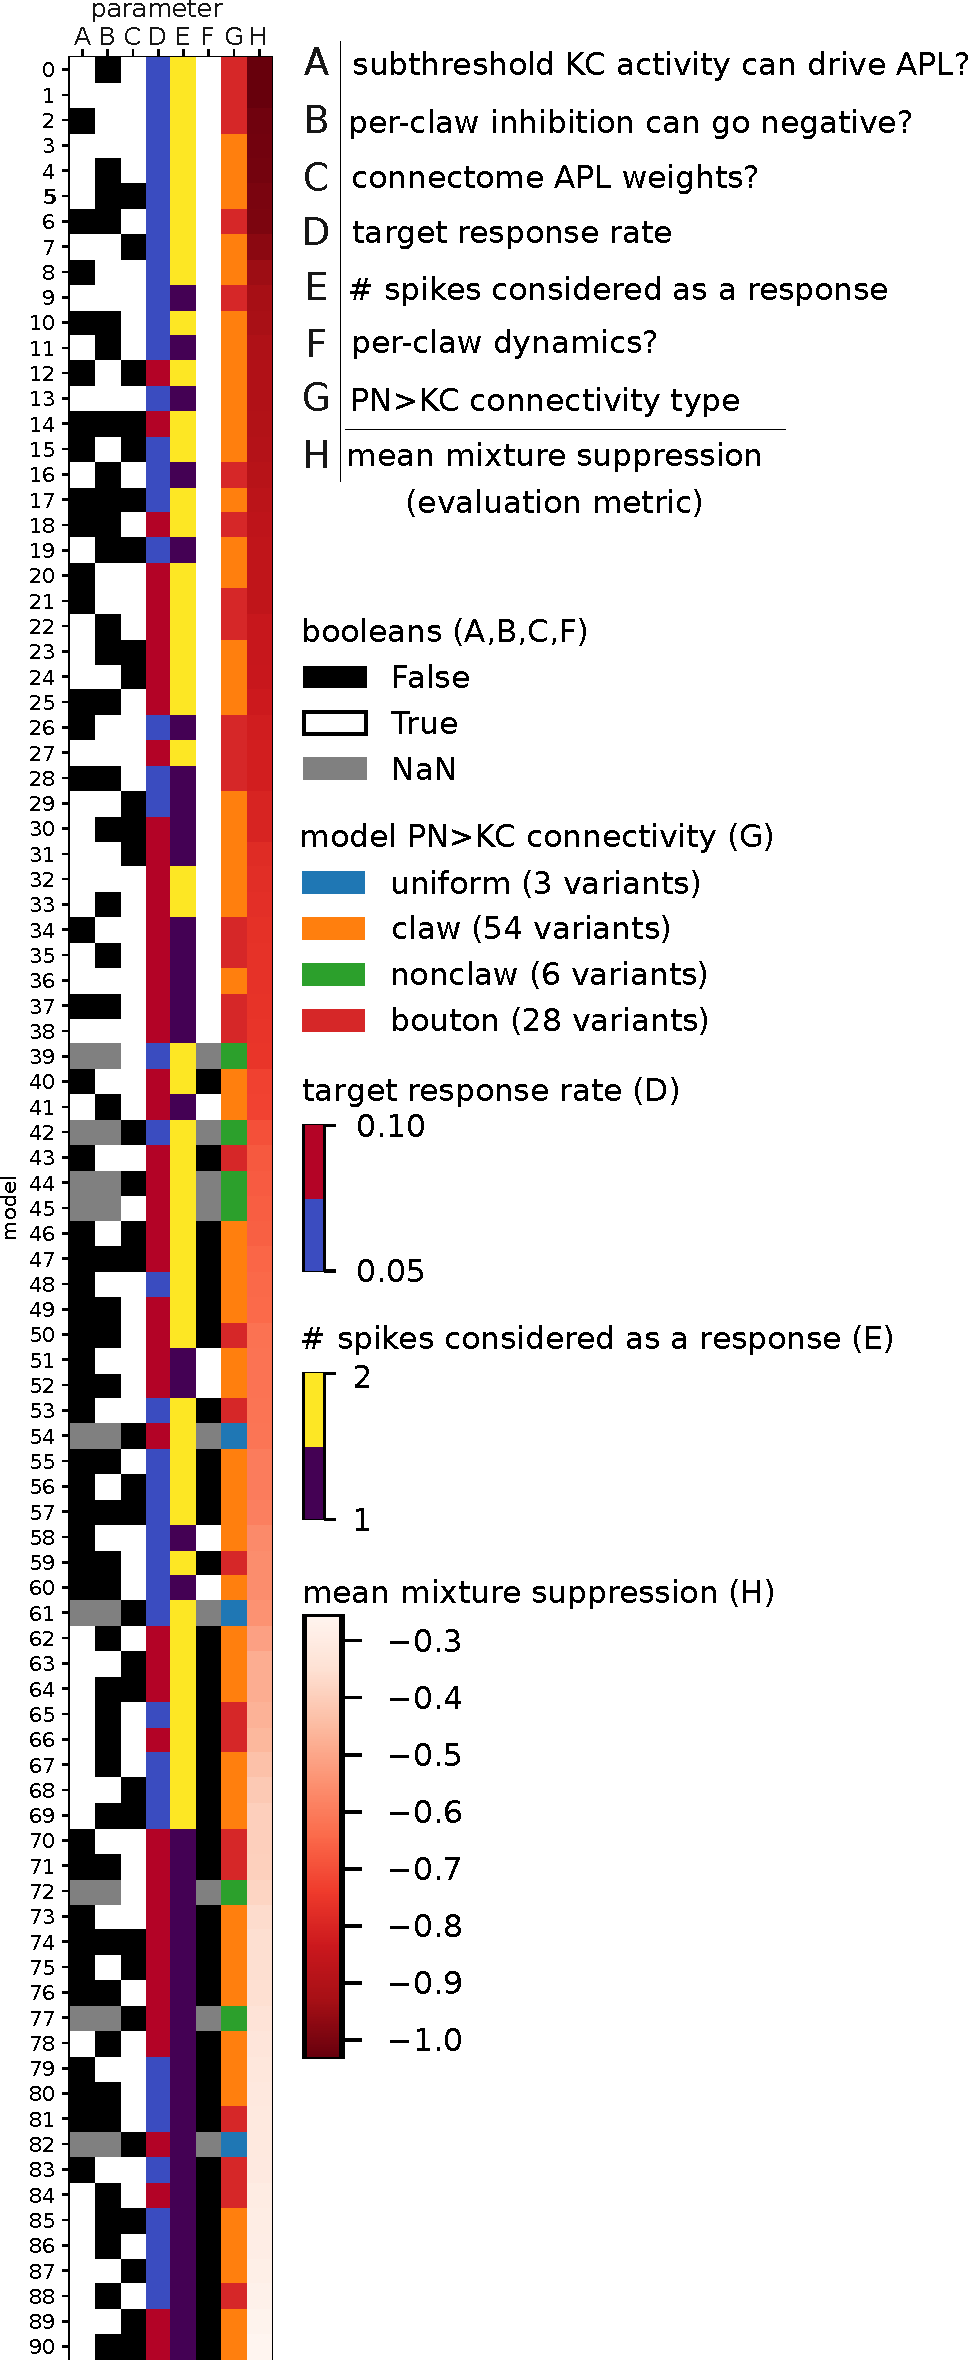
\includegraphics[height=0.9\textheight]{models-with-params_sorted-by-mean-mixsupp}
\mycaptionof{figure}{Model parameters sorted by mean mix A \& B mixture suppression}{%
% TODO also change so NaN gray values are replaced with the most appropriate True/False value (at least for A/B [pn_claw_to_apl/allow_net_claw_inhibition]. F=claw_dynamics can stay NaN in relevant cases)? care?
Rightmost column (H) is mean mixture suppression (within mix A \& B, both 2 \& 5-components, although the larger 5-component values dominate), and all model variants are sorted by this value.\\~\\
% TODO move some or all of below text into methods text, and then link to this fig?
The model variant discussed in this chapter is model 5 (with the bold ID number).
It takes advantage of setting options only available to models with discrete claws (``claw'' / ``bouton'' versions): A=true and B=false.\\~\\
Model 15 may be more comparable to the behavior of older model variants (``nonclaw'' / ``uniform''), because it sets A=false \& B=true, which was the only behavior available in these older models.
Like model 5, model 15 does also take advantage of the discrete-claw specific parameter that allows per-claw dynamics (and time constants) that older model variants lacked.
Model 15 still has a significantly higher mean mixture suppression than the models with the most suppression in either the ``nonclaw'' or ``uniform'' cases (models 39 and 54, respectively).
I expect that most mixture suppression effects would remain if the model 15 were used in place of model 5.\\~\\
None of the ``bouton'' models, which have separate bouton units and \APLBouton weights (also from the hemibrain connectome), outperformed any of the ``claw'' models enough to justify the additional complexity.
}
\label{fig:models-with-params_sorted-by-mean-mixsupp}
\end{longcapfigure}
% }

\subsubsection{Processing connectome data}
\label{sssec:connectome_weights}
Skeletons and synapses of right-hemisphere KCs that received olfactory PN inputs, the PNs that contacted those KCs, and the right anterior paired lateral (APL) neuron were obtained from the hemibrain connectome (v1.2.1; neuPrint; NAVis).
After skeleton healing (rejoining cuts introduced by skeletonization of the segmented volume), each arbor was restricted to the right MB calyx by retaining the portion that lay outside a custom exclusion mesh covering non-calyx compartments.
KCs were restricted with one mesh, while the PNs and APL were restricted with a revised version of that mesh.
Synaptic connectors on these calyx arbors were then grouped into anatomical units using geodesic distance along the skeleton, computed in hemibrain raw coordinates (\qty{8}{\nano\metre} per voxel).
Isolated synapses whose mean geodesic distance to their ten nearest neighbors was \qty{6.0}{\micro\metre} or greater were discarded as stragglers.
The remaining synapses were clustered by treating pairs within \qty{6.8}{\micro\metre} as connected and taking the connected components of this graph.
% TODO what was this cap (or were these caps?)? (oh, discussed in next paragraph?)
% TOOD what minimum size?
Clusters that exceeded a cell-type-specific synapse cap were further split by constructing a $k$-nearest-neighbor minimum spanning tree and iteratively cutting an edge, provided that both resulting components remained above a minimum size.

For KC claws, oversized clusters were split at a target cap of 40 synapses (minimum size 6), after which assignments were refined using PN identity: (a) claws contacted by more than one PN were split so that each claw received input from a single presynaptic partner; (b) unassigned PN synapses were absorbed into that PN's existing claw on the same KC, or used to seed a new claw if they comprised more than five contacts; and (c) corrected labels were propagated to nearby unlabeled synapses within \qty{12.8}{\micro\metre}.
The number of claws per KC was defined as the number of these corrected clusters with at least five synapses.
PN boutons were segmented without this minimum-spanning-tree splitting step, using a tighter isolation threshold (mean distance to the five nearest neighbors below \qty{2.8}{\micro\metre}) and a \qty{4.8}{\micro\metre} clustering cutoff.
APL calyx arbors were segmented with the same geodesic procedure as KCs but with a larger target cap of 50 synapses and a minimum split size of 10. 
%The resulting clusters are referred to as anatomical units.

Thanks to Pratyush Kandimalla for implementing the anatomical connectome segmentation described above.

\subsubsection{Scaling model spike counts to make comparable to KC measurements}
\label{sssec:scaling_spike_counts}
We apply a logistic function to the model spike counts to bring the data range roughly in line with the KC measurements, so that subtracting responses to two odors should give us mixture suppression values in a similar range.
If we were to use raw spike counts, we would get dramatically more mixture suppression, but only because a small number of high spiking cells get dramatically suppressed, not because of any change in the majority of cells that only spike once or twice.
It also mirrors the saturation we expect both due to several possible biological mechanisms and also because of the saturating nature of our calcium imaging readout of KC spiking.
If there truly were a small subpopulation of high spiking KCs, it could only be because of our imaging methods that we cannot resolve their increased responses above cells that spike a more modest amount.

For a logistic function of the form: $f(x) = \frac{L}{1 + e^{-k(x-x_0)}}$ the current parameters we use to scale the model spike counts are $k=2$, $x_0=2$, $L=3$, which starts at essentially 0 for no spikes, crosses the midpoint of 1.5 at 2 spikes, and saturates after about 4 spikes.
Across the KC mix A \& B data, a \KCRespStat{ }value of 3 (where this scaling saturates) corresponds to the \textasciitilde$97^{th}$ percentile of the observed KC responses, which seems like a reasonable match to the upper limit of the KC data.
% TODO delete last bit about unspecified sensitivity analysis?
We had also tried other variants that saturate at higher numbers of spikes (\textasciitilde10) with similar results (data not shown).

% TODO TODO delete? or refer to in supplemental intensity figs, at least?
\subsubsection{Comparing mean response intensity across model and measured KC responses}
\label{sssec:model_vs_kc_intensity}
% TODO try to reduce whitespace after \geq?
% https://www.overleaf.com/learn/latex/Spacing_in_math_mode#Operators_spacing
For measured KC responses, the mean response rate is defined via thresholding described previously, while the model responses are defined by whether or not each model cell fired $\geq2$ spikes to an odor, with the mean response rate then calculated across all cells for each odor (as elsewhere).

For measured KC responses, the ``normalized'' mean response starts with the same \KCRespStat, as in the plots only analyzing mean measured KC response intensity, and scales all data (within a particular mixture, if a dataset has multiple) so that the odor with the highest mean response has a mean response of 1.
The ``normalized'' model mean response starts with the logistic-scaled spike counts (as described in previous methods section), and then scales all data for each model variant so its max odor response is 1.

% this call is just to handle any plots in methods, in particular the model params one w/ H placement,
% which would screw other plots up (w/ endfloat enabled, at least), if there was not a prior \processdelayedfloats
% call before methods
\processdelayedfloats
% so references start on a next page. no empty page currently inserted between caption of model param plot and this
% (w/ endfloat enabled, at least)
\clearpage
%

\ReferencesSection
\end{refsection}

% Supplemental Figures/Tables
% TODO can these `% {` / `} %` blocks be nested? is a nested block below the reason this isn't working?
% {
\supplementsection
% TODO move model param fig down here too? (the one from methods)

\begingroup
% (1.9 rather than 2.0, so this table fits on one page along w/ the section heading. otherwise it ran past
% the bottom margin, and the page before it was empty except for the heading's link target.)
\renewcommand{\arraystretch}{1.9}

\newcommand{\LoadChemFigWithScale}{\LoadChemFigTexFromCID[scale=0.9]}
\newcolumntype{Z}{>{\collectcell\LoadChemFigWithScale}p{1.9cm}<{\endcollectcell}}

\newcolumntype{R}{>{\collectcell\cid}p{1.4cm}<{\endcollectcell}}

% TODO TODO or just move to stimulus choice section? (or stimulus/odor methods?)
% TODO include vapor pressures for all i can? (+ pubchem links?)
% TODO TODO add CIDs here too (but how to get it to not apply to mix rows?) can i easily?
% use multirow inside table?
\begin{longcaptable}
\centering
% anything less than 2.8cm (checked down to 2.75cm) currently splits "methyl salicylate" awkwardly
\begin{tabular}{p{1.1cm}p{2.8cm}p{1.25cm}p{1.35cm}RZ}
% TODO bold everything?
% TODO delete if auto bolding good
%\textbf{Mix} & \textbf{Name} & \textbf{Abbrev.} & \LogConcXBold\footnotemark[1]{} & \multicolumn{1}{l}{\textbf{CID}} & \multicolumn{1}{l}{\textbf{Structure}} \\
% TODO delete. auto bolding did not work
Mix & Name & Abbrev. & \LogConcX\footnotemark[1]{} & \multicolumn{1}{l}{CID} & \multicolumn{1}{l}{Structure} \\
\midrule
  & paraffin oil & pfo & & & \multicolumn{1}{c}{} \\
\hline
\multirow{6}{*}{A}
 &         ethanol &    EtOH &          -2 &   702 &       702 \\
 & isoamyl alcohol &    IAol &        -3.6 & 31260 &     31260 \\
 & isoamyl acetate &     IaA &        -3.7 & 31276 &     31276 \\
 &   ethyl acetate\footnotemark[2]{} &      ea &        -4.2 &  8857 &      8857 \\
 &  ethyl butyrate\footnotemark[2]{} &      eb &        -3.5 &  7762 &      7762 \\
% try something like this, to make line ligher (gray instead of black?)?
% https://tex.stackexchange.com/questions/527455/get-current-value-of-arrayrulecolor-for-a-colortbl
% how to reset arrayrulecolor, or only set locally though? is black default?
% (eh, \hdashline is fine)
\hdashline
% TODO say in-vial?
  & \makecell{5 components\\above, mixed} & kmix & & & \multicolumn{1}{c}{} \\
\hline
% https://tex.stackexchange.com/questions/65127
% for extra space for ms structure
\rule{0pt}{2.3\normalbaselineskip}
\multirow{6}{*}{B}
 & methyl salicylate &       ms &          -3 &  4133 &      4133 \\
 &      valeric acid &       va &          -3 &  7991 &      7991 \\
 &          furfural &      fur &          -4 &  7362 &      7362 \\
 &       2-heptanone\footnotemark[2]{} &       2h &          -5 &  8051 &      8051 \\
 &      1-octen-3-ol\footnotemark[2]{} &    1o3ol &          -3 & 18827 &     18827 \\
\hdashline
%  & 5 components above, mixed & cmix & \\
  & \makecell{5 components\\above, mixed} & cmix & & & \multicolumn{1}{c}{} \\
\hline
% need the second arg? (yes) need something in there? (yes)
% (empty doesn't work, and no second arg also doesn't seem to work)
% "\\" not allowed in multirow 3rd arg, it seems (LR mode)
% "* [for 2nd arg] to use natural width of content"
% https://tex.stackexchange.com/questions/73283/how-to-use-multirow
\multirow{3}{*}{\makecell{weak\\binaries}}
% i don't think i actually used the 5 flies with -2.5 for farnesol, cause i always report N as 12 and there are 12 w/ just farn -3
% oh, i think i did, but it was just a subset of the 12 flies that also had -2.5?
% TODO how to get there not to be spacing after 2-heptanone row above? ideally want "weak binaries" centered vertically in space, with equal space between all "Common name"/etc values here
 & 2-heptanone & 2h & -7 & 8051 & 8051 \\
 & farnesol\footnotemark[3] & farn & -3 & 445070 & \multicolumn{1}{l}{\LoadChemFigTexFromCID[scale=0.73]{445070}} \\
 & methyl acetate & ma & -7 & 6584 & 6584 \\
\bottomrule
\end{tabular}
% TODO rename (back to "Odor abbreviations"?) if i end up including megamat/etc odors here (i prob won't)
\mycaptionof{table}{Mixes and their components}{%
All of these odors use paraffin oil as their solvent.
% TODO TODO add note about how the weak-binaries component concentrations differ from those in diagnostic panel
}
\label{table:mix_odors}
\index{tables}
\end{longcaptable}
% TODO delete either this or duplicate below? can i omit the actual text on the second one?
\footnotetext[1]{In-vial v/v concentration.}
% TODO be consistent about whether to end these in periods or not
\footnotetext[2]{Also components of binary mixture}
% TODO TODO keep/delete?
%\footnotetext[3]{5 of the 12 flies also had farnesol at -2.5, and all mixtures with that concentration (and all with -3). That data was also included.}
\footnotetext[3]{5/12 flies had farnesol at -2.5 as well as -3 (and all mixtures with both). -2.5 data included too.}
\endgroup

\begin{longcapfigure}
\centering
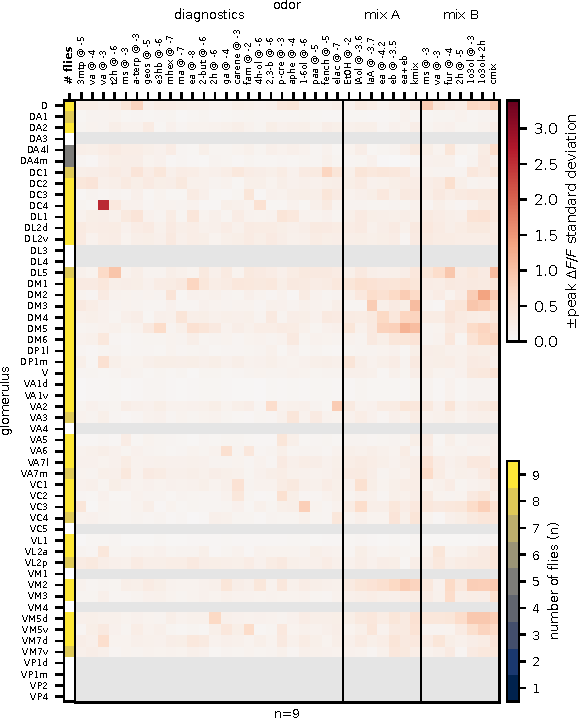
\includegraphics[height=0.68\textheight]{orn_responses_stddev_and_n}
\mycaptionof{figure}{ORN response standard deviation and per glomerulus fly counts}{%
Standard deviation (across flies) for the responses shown in \cref{fig:orn_mean_responses}.
The color scale is the same as the positive side of the color scale in that mean response plot.
The leftmost column contains the \# of flies in which each glomerulus is
identified, or white for those not identified in any flies.
% TODO move to text?
The vast majority of glomeruli respond relatively consistently across flies, to the majority of odors.
Most odors have reasonably consistent responses across flies, and most glomeruli were identified in all 9 flies, with the least sampled glomerulus analyzed still identified in 5 flies.
The flies have \numrange{38}{42} glomeruli identified, with a mean of 41.2.
A small number of glomeruli identified in less than half of the flies were excluded from analysis
}
\label{fig:orn_stddev_and_n}
\end{longcapfigure}

% TODO TODO edit to delete uniform model (or just keep out)
% TODO figure out what i want to do with this. add back some version of (maybe count version of) mix vs top component plot?
% TODO is it actually worth showing these? density doesn't really seem any better...
% maybe i should focus on the top component vs mix after all? (don't think that made any more impression of an effect really)
%\begin{figure}
%\centering
%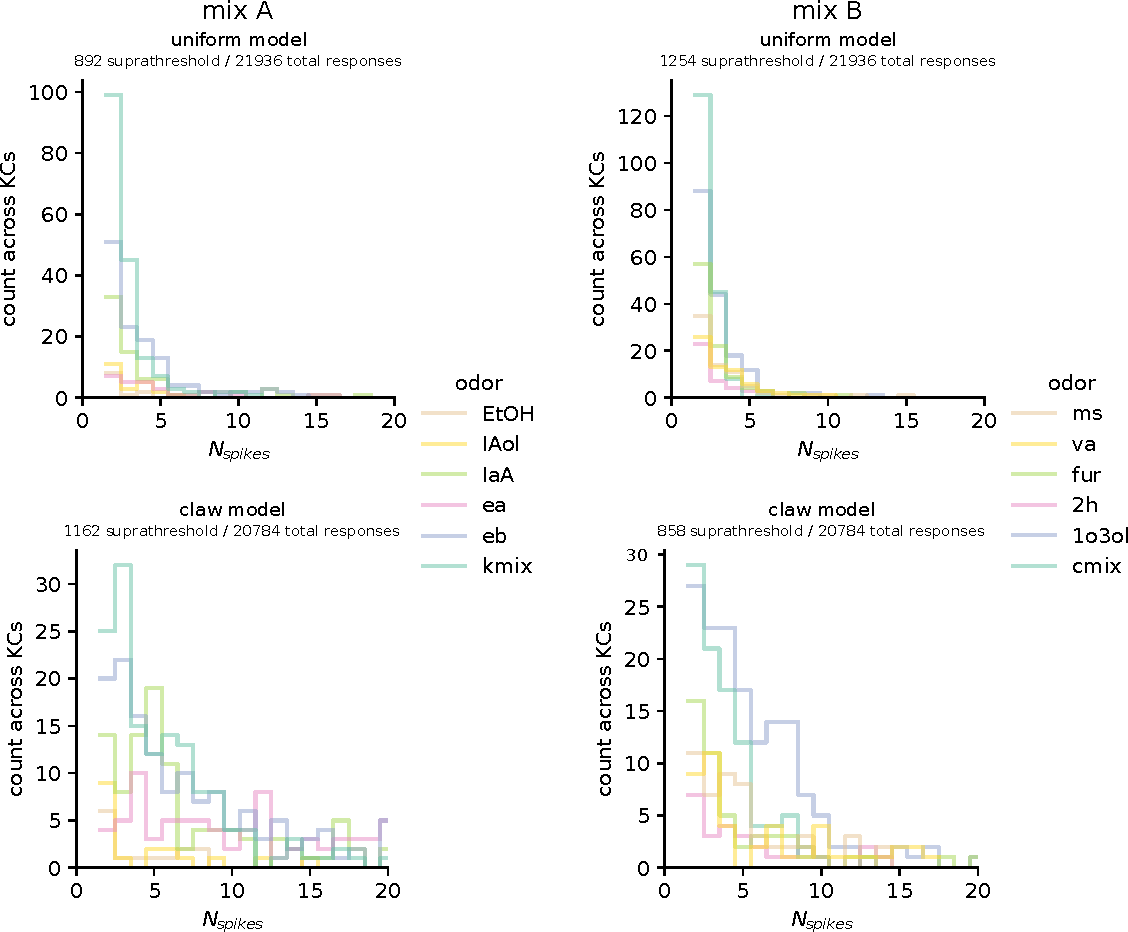
\includegraphics[width=\textwidth]{perodor-response-strengths_model_counts_5comp}
%\captionbacktorefs{Per-odor distributions of model \NSpikes, for 5-component mixes}{fig:perodor_model_counts_5comp}
%Unlike the similar distributions before, showing KC \& ORN data, all parts of this plot exclude non-responding model cells.
%\end{figure}
%\begin{figure}
%\centering
%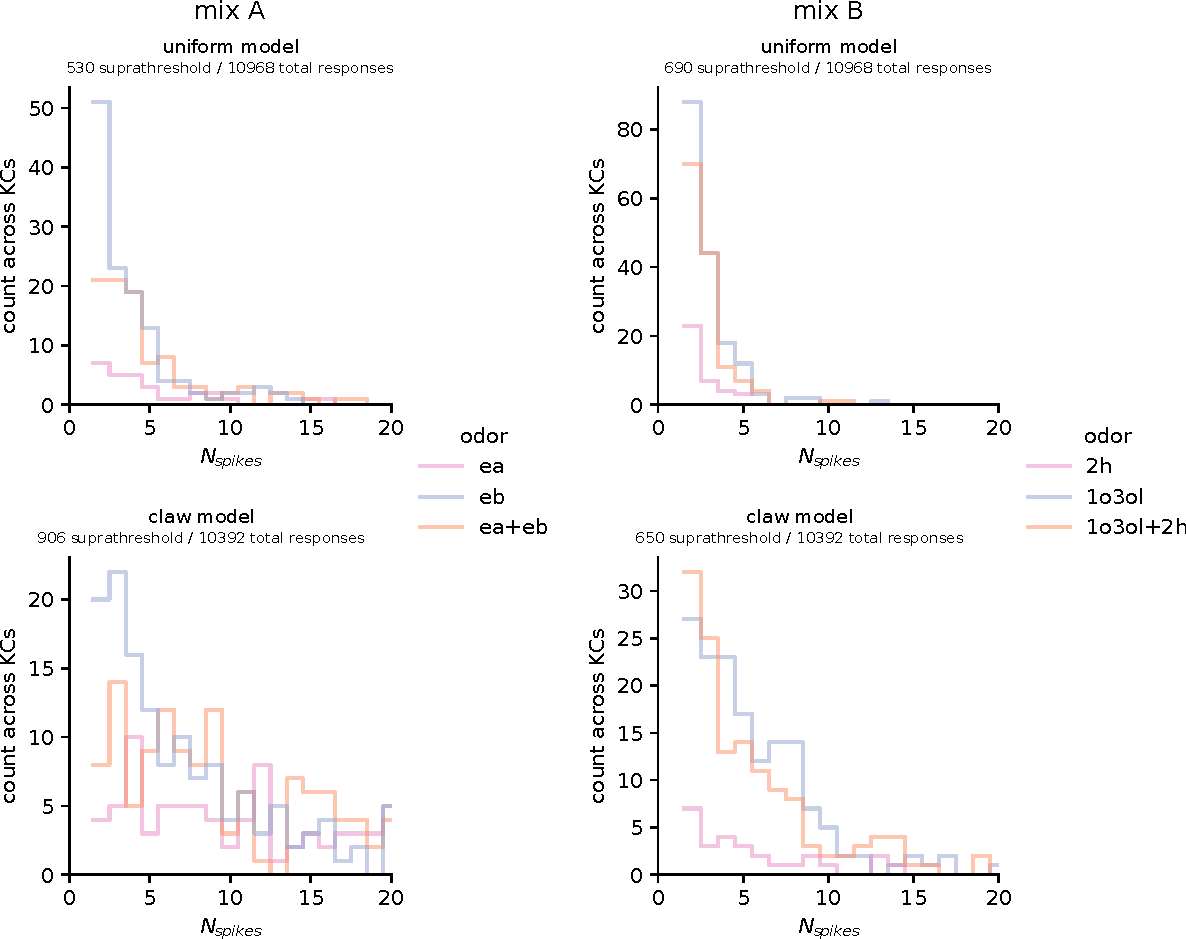
\includegraphics[width=\textwidth]{perodor-response-strengths_model_counts_binary}
%\captionbacktorefs{Per-odor distributions of model \NSpikes, for 2-component mixes}{fig:perodor_model_counts_binary}
%% TODO add text
%\end{figure}
%

% Model vs KC intensity (mix A/B)
% {
\begin{longcapfigure}
\centering
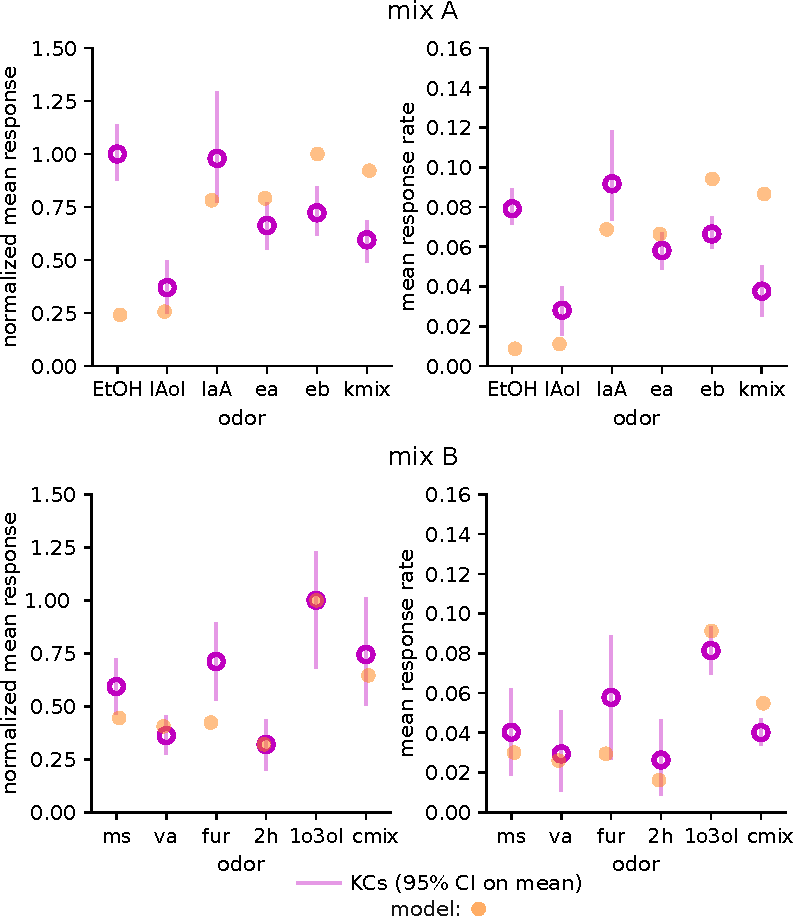
\includegraphics[height=0.7\textheight]{intensity_model-vs-kcs_logistic-scaled_5comp}
\mycaptionof{figure}{KC and model average responses to five-component mixtures}{%
Left: response strength separately normalized both in KC (\KCRespStat) and model (logistic-scaled spike counts) data.
% TODO link specific part of methods (/delete)
See Methods for normalization details.
Right: raw mean response rates to each odor.
% TODO link specific parts of methods
See Methods for how response rates are defined.\\~\\
Note that mismatches for EtOH, IaA, fur seem to follow from weaker ORN responses to these odors (\cref{fig:intensity_orn-vs-kc}).
The model may slightly improve on the ORN intensity mismatch for 1o3ol (and perhaps slightly for IaA), but it also seems to overpredict the relative responsiveness to eb.
}
\label{fig:intensity_model-kc_5comp}
\end{longcapfigure}

\begin{longcapfigure}
\centering
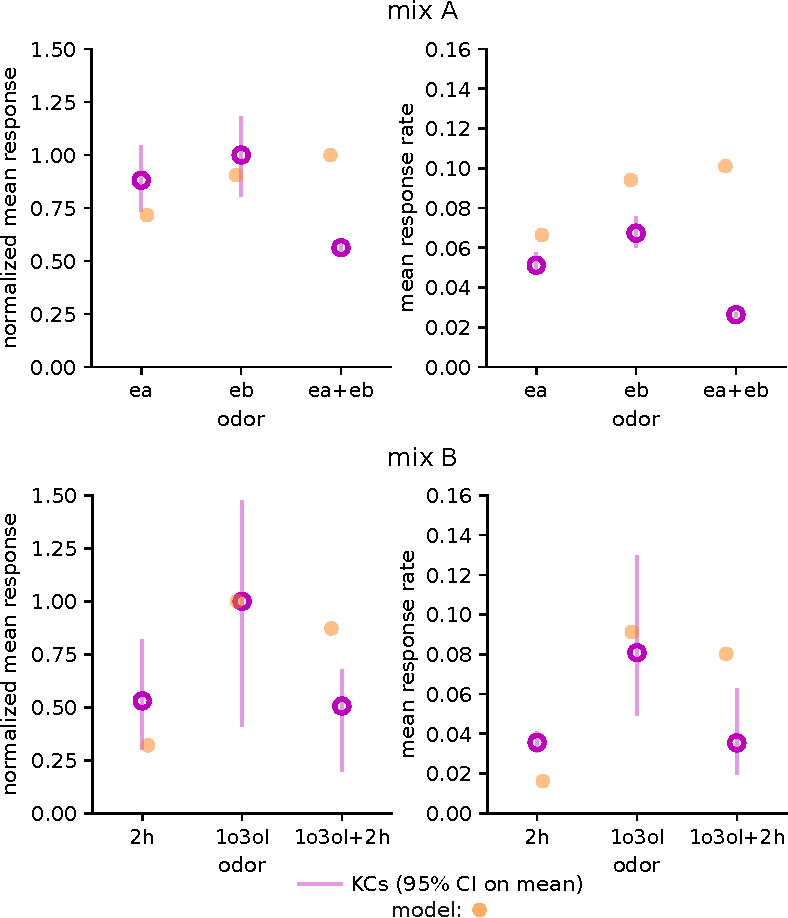
\includegraphics[height=0.7\textheight]{intensity_model-vs-kcs_logistic-scaled_binary}
\mycaptionof{figure}{KC and model average responses to binary mixtures}{%
See \cref{fig:intensity_model-kc_5comp} for details.
}
\label{fig:intensity_model-kc_binary}
\end{longcapfigure}
% }

% TODO refer to these (/delete?)? at least in caption of plot that also has ORN response classes?
\begin{longcapfigure}
\centering
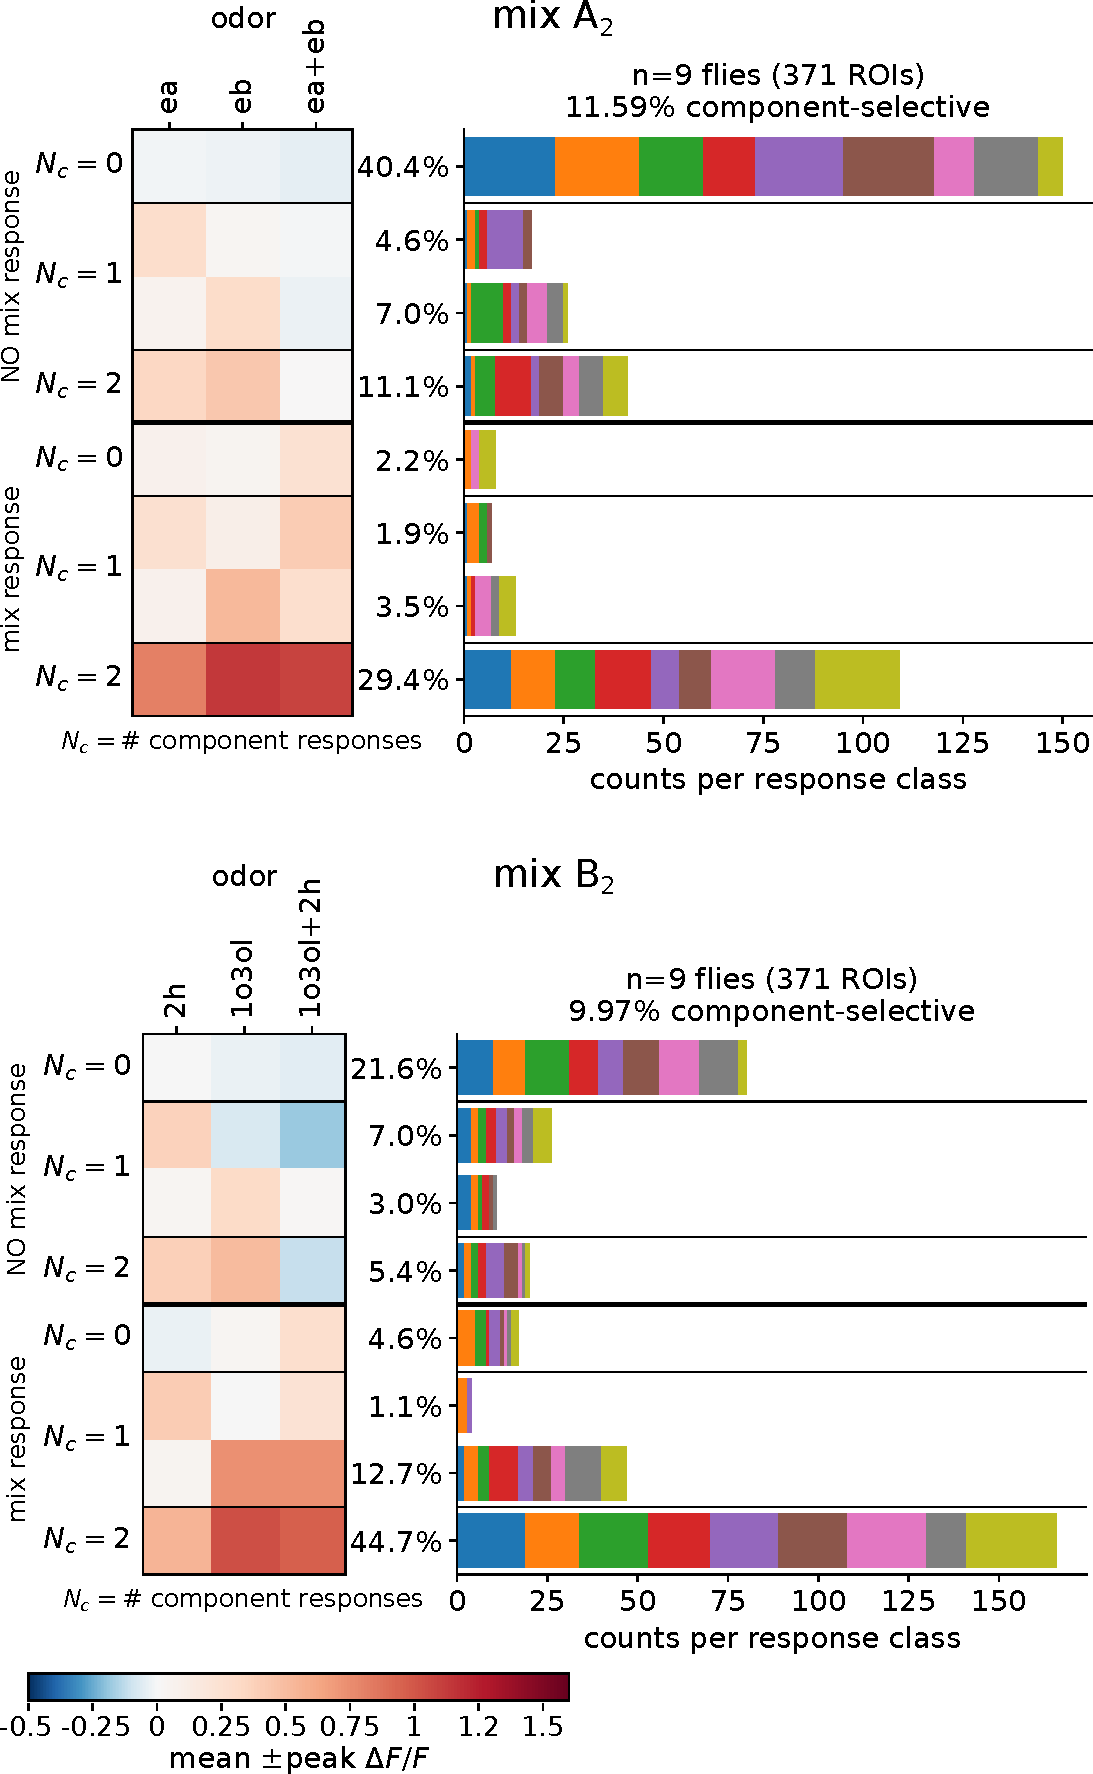
\includegraphics[height=0.85\textheight]{response-class-means_orn_binary}
\mycaptionof{figure}{ORN 2-component mix response class means and counts}{%
Left: mean responses across all glomeruli within a response class.
Right: counts of this response class, across glomeruli from all flies.
Different colors in right panel bars correspond to different flies.
}
\label{fig:response-class-means_orn_binary}
\end{longcapfigure}

\begin{longcapfigure}
\centering
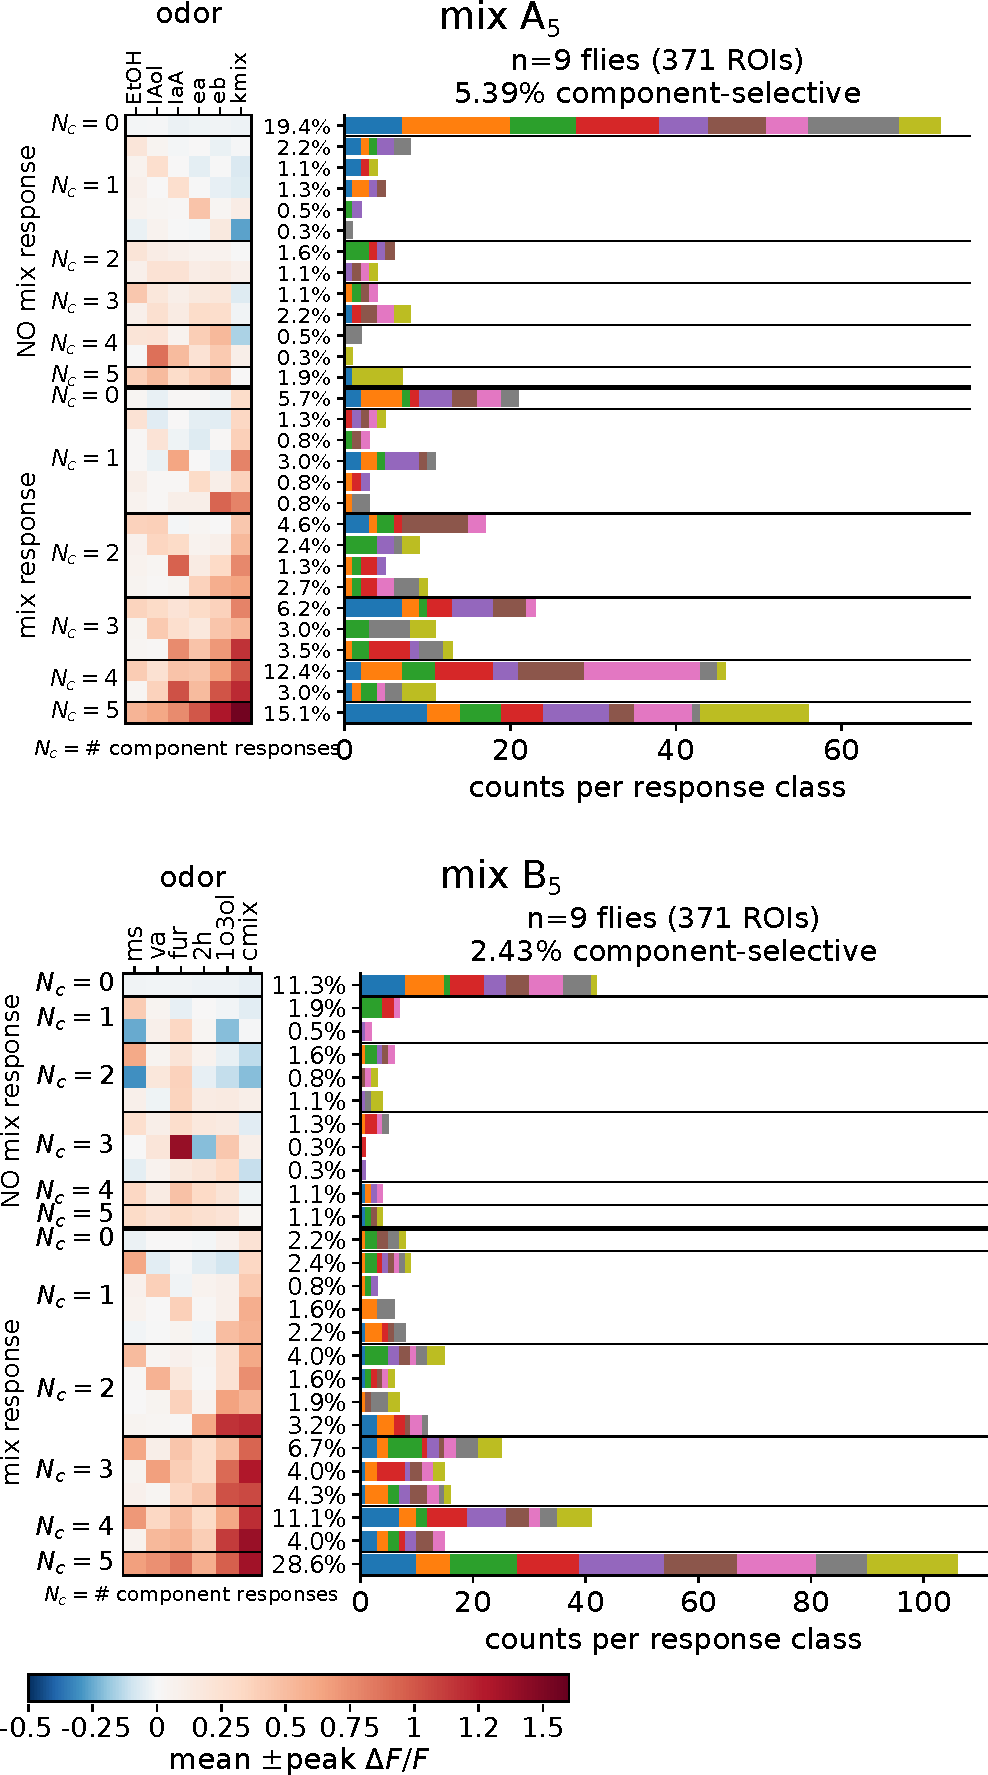
\includegraphics[height=0.85\textheight]{response-class-means_orn_5comp}
\mycaptionof{figure}{ORN 5-component mix response class means and counts}{%
As \cref{fig:response-class-means_orn_binary}, but for 5-component mixtures.
}
\label{fig:response-class-means_orn_5comp}
\end{longcapfigure}

% TODO TODO delete (or at least regenerate to only use claw model, not uniform)
%
% TODO put these in appendix or something? other than 1.5 percentage point increase (~50% relative) in segmenting cells (claw vs uniform, and only in mix A case) none of the binary models are any good. claw model also does worse in some aspects of binary mix A, in adding many more mix + component responders.
%\begin{figure}
%\centering
%\includegraphics[width=\textwidth]{response-class-mean_model_binary_kiwi}
%\captionbacktorefs{Model 2-component mix A response class means and counts}{fig:response-class-means_model_binary_kiwi}
% % TODO caption
%\end{figure}
%\begin{figure}
%\centering
%\includegraphics[width=\textwidth]{response-class-mean_model_binary_control}
%\captionbacktorefs{Model 2-component mix B response class means and counts}{fig:response-class-means_model_binary_control}
% % TODO caption
%\end{figure}

% for supplement figures
\processdelayedfloats
% TODO clearpage/newpage here?
% }

\chapter{General Discussion}
\begin{refsection}
\label{chap:discussion}

%Across the work in this thesis, some of the biggest unresolved questions relate to the role of specific elements in our MB model, as well as the importance of particular odors (or odor pairs).
Across the work in this thesis, some of the biggest unresolved questions relate to the role of specific elements in our MB model, as well as the importance of particular odors.
In some cases in silico work may be sufficient to clarify the role of certain model elements, but in some cases we may need additional measurements of key circuit elements (e.g. the APL or MB-C1) to clarify whether and how the model should be updated to better capture their role in shaping KC responses.
Whether certain odor pairs have outsized effects in the remappings we see in \autoref{chap:remypaper} could potentially be uncovered with new analysis, but it will likely take new experiments with new odor mixtures to understand the peculiar behavior we seem to see in response to our mixtures in \autoref{chap:natmix}.

In \autoref{chap:remypaper}, we find some hints that structure in the connectome PN-to-KC weights is involved in aligning KC odor representations with odor distances in natural sources.
%Beyond the question of what changes could be made to the model to account for the remainder of the remapping we see in the KCs, the `hemibrain' model in that chapter needs some additional comparisons to clarify what level of structure in the PN-to-KC weights is 
The `hemibrain' model in that chapter needs some additional comparisons to clarify what components of PN-to-KC structure are important for this remapping.
In the version of this work presented in this thesis, the only comparison is to the `uniform' model variant, in which each KC has a fixed number of glomerular inputs (``claws''), from a uniform distribution across glomeruli.
Some earlier versions of the modeling in that chapter also made comparisons to a `hemidraw' variant, which was also drawing 7 inputs per KC, but from a distribution where the probability of drawing each glomerulus was computed from an earlier version of the connectome data.

In theory, this comparison was intended to isolate the effect of the probability of drawing each glomerulus (i.e. how many boutons each glomerulus has in the PN outputs in the CA) from the effect of KCs over/under-sampling particular combinations (e.g. pairs) of glomeruli, as it has been well established that there are particular pairs of glomeruli that KCs sample at rates above and below chance\cite{CommunityPNs}.
The latest `hemidraw' variant was limited in two main ways.
First, it only sampled a fixed number of inputs per KC, rather than using the known distribution of how many inputs each KC receives.
Second, while the `hemibrain' model has had the PN-to-KC weights updated based on newer analyses, the code behind the `hemidraw' variant was never updated to use per-glomerulus probabilities computed from this latest analysis of the connectome.
As such, it remains unclear to what extent the slight remapping the `hemibrain' model contributes is specifically because of the biased sampling of particular pairs of glomeruli.

Another unresolved question in \autoref{chap:remypaper} is the importance of specific odor pairs, and whether it is the outsized influence of a few such odor pairs that explains much of the KC representation alignment with natural source distances.
Although we do resampling across odor pairs to demonstrate that our effects are at least somewhat robust to the exclusion of certain subsets of odors, we do not design analyses specifically to identify particular odor pairs that contribute more to the overall remapping.
It would be especially interesting if we could independently identify such pairs of odors, either by analysis of natural odor data (e.g. VCF or MetaCyc) or by analysis of biases in the PN-to-KC connections (that seem to account for at least some of the ORN-to-KC remapping).

In \autoref{chap:natmix}, the biggest mystery is why we see such pronounced KC mixture suppression to our five-component mixtures (notably more than to our binary mixtures), if KCs tend to exhibit robust responses to natural odors (which should be even more complex), as in \textcite{Honegger2011} as well as unpublished data from our lab.
Perhaps KCs really do tend to exhibit more mixture suppression to mixtures with more components, but there is some parallel mechanism which keys in to specific features of natural mixtures, restoring robust responses specifically to these stimuli?
Or maybe there is something unfortunate about our specific choice of two mixtures, and the strong KC mixture suppression we see would not tend to generalize to additional mixtures with greater diversity?
I think we will need a combination of additional experiments to get clarity, starting with more diverse five-component mixtures.
Ultimately, I think we will want to do similar experiments with mixtures that try to bridge into the complexity and ideally recreate the percept of particular natural stimuli.

An ongoing effort by another graduate student in our lab has now developed a combination of volatiles that seems to reasonably well approximate the ORN representation and behavioral responses elicited by banana, so it would be interesting to record KC responses to this mixture.
Does banana itself evoke similarly strong KC responses to other natural stimuli we have measured before?
If so, does this complex banana approximation also show robust KC responses, or does it show more mixture suppression as with our five-component mixtures?
If we start with mixtures that are simpler subsets of this full mixture, and add more components to approach the full percept, do we see mixture suppression along the way, which ultimately gets reversed somehow by the time we well approximate the natural stimulus?
The easiest way to do these experiments at scale may be to adopt the GC-Recomposition-Olfactometry (GC-R) approach of \textcite{GCRecombination1}, as we have most of what we would need to accomplish this in our lab already.
However, this would certainly still pose many challenges, and be difficult to fit into our existing imaging setups.

Another outstanding mystery in the \autoref{chap:natmix} data is the dramatically increased response to ethanol, which seems to elicit strong KC responses despite weak ORN responses.
Ethanol is an ethologically important odor for flies, given that they feed off of the yeast that would give off ethanol as a byproduct, so it makes sense that there might be some mechanism to boost the response of this odor in the KC representation.
Uncovering the mechanisms behind the boost of the ethanol response may also shed light on why natural odors elicit robust KC responses, and one neuron which seems like it could contribute to such modulation of KC responses is the MB-C1 neuron, which is inhibitory to KCs while also receiving at least some inputs from the LH.
There is ongoing work in the lab to characterize the response of this neuron to many odors, and it would be interesting to see if it has a role in boosting weak ethanol or natural mixture responses.

\ReferencesSection
% TODO TODO so do i need something else to have one overall bibliography? is that a requirement (if not, whatever)
% (currently there is a warning this one is empty) (if not a requirement, prob fine to delete this one)
%\printbibliography[heading=bibintoc]
\end{refsection}

% TODO want anything in here?
% TODO order of \appendix and \chapter matter?
% TODO where should appendix figures go?
\appendix
% this will make an "Appendix A". the appendix command above does not actually put some text that says "Appendix" anywhere in the document. it would just throw everything after the bibliography above, without manually making a new chapter or something
\chapter{}
% TODO delete? keep?
\label{chap:appendix}

\newpage

\begin{landscape}
\begin{longcaptable}

% TODO try multipage longtable instead of rotating? https://www.overleaf.com/learn/latex/Tables
% single spaced, w/ slightly less space between rows, so this table fits on the landscape page along w/ its
% caption and footnote. (rows were too tall w/ the document's 1.5 spacing: the table ran past the bottom margin,
% and the page before it was empty.)
{\SingleSpacing*\renewcommand{\arraystretch}{0.94}
\begin{tabular}{llcllU}
% TODO also include where we ordered from (or sigma product IDs + links, for the vast majority [all?] where that's where we ordered from)?
%Common name & $\log_{10} \text{concentration}$ & \parbox{2cm}{Target glomerulus} & Solvent & PubChem ID\\
% TODO rename this 'PubChem ID' -> CID (to save space, and for consistency w/ above)?
%
% TODO link to DoOR for glomeruli? meh
Common name & Abbreviation & \LogConcX\footnotemark[1]{} & Target glomerulus & Solvent & \multicolumn{1}{l}{CID}\\
\midrule
3-methylthiopropanol & 3mtp & -5 & DM3 & pfo & 10448\\
valeric acid & va & -4 & DM6 & water & 7991\\
trans-2-hexenal & t2h & -6 & DL5 & pfo & 5281168\\
methyl salicylate & ms & -3 & DL1 & pfo & 4133\\
alpha-terpineol & a-terp & -3 & D & pfo & 17100\\
perfume geosmin & geos & -5 & DA2 & pfo & 1213\\
ethyl 3-hydroxybutyrate & e3hb & -6 & DM5/VM5d & pfo & 62572\\
methyl hexanoate & mhex & -7 & DM2 & pfo & 7824\\
methyl acetate & ma & -7 & DM4 & pfo & 6584\\
ethyl acetate & ea & -8 & DM1 & pfo & 8857\\
2-heptanone & 2h & -6 & VM5d & pfo & 8051\\
geranyl acetate & ga & -4 & VA6 & pfo & 1549026\\
valeric acid & va & -3 & DC4 & water & 7991\\
(1S)-(+)-carene & carene & -3 & DC1 & pfo & 443156\\
farnesol & farn & -2 & DC3 & pfo & 445070\\
4-heptanol & 4h-ol & -6 & VM2 & pfo & 11513\\
2-butanone & 2but & -6 & VM7d & pfo & 6569\\
2,3-butanedione & 2,3-b & -6 & VA2 & pfo & 650\\
p-cresol & p-cre & -3 & VC2 & pfo & 2879\\
acetophenone & aphe & -4 & VA3 & pfo & 7410\\
ethyl lactate & elac & -7 & VC4 & pfo & 7344\\
1-hexanol & 6ol & -6 & VC3 & pfo & 8103\\
phenylacetaldehyde & paa & -5 & VL2a & pfo & 998\\
fenchone & fench & -5 & VC1 & pfo & 82229\\
\bottomrule
\end{tabular}
}
% (before the caption, so the space for it is accounted for when checking whether the caption fits)
\footnotetext[1]{In-vial v/v concentration.}

\mycaptionof{table}{Diagnostic odors used to assist in identifying and segmenting glomeruli}{}
% TODO also refer to full volume images if i include those? (in remypaper supplemental figures now. 2 pages)
% TODO compare hyperlink's \autoref and cleveref \cref for this and tables?
%See \cref{fig:s1} for example volumetric responses to this full panel in one fly from \autoref{chap:remypaper}.
%See left side of \cref{fig:orn_mean_responses} for some example mean responses to these odors.
\label{table:diagnostic_odors}
\index{tables}
\end{longcaptable}
% TODO mention we chose nearest log10 v/v dilution when picking mix B odor concentrations (for approximate intensity matching)?
% TODO TODO mention boosting ethanol and why (and from what measured value?). in footnote here or in text?

\end{landscape}

% TODO want either of these
%\chapter{Questionnaire}
%\chapter{Consent Form}

% TODO want?
% TODO TODO delete all index commands above? not sure this is helpful at all
% (and still not clear on if i need to specify multiple figures, or if i even went the figures in the index. we already have list(s) of figures...)
%\printindex

% end notes not displayed without this
%\theendnotes

%% Pocket materials at the VERY END of thesis
%\pocketmaterial
%\extrachapter{Pocket Material: Map of Case Study Solar Systems} 

\end{document}
